\documentclass[11pt]{article}
\usepackage{mystyle}

\title{FIT1058 --- Notes\\
\large Course Note(CN) $+$ Rosen Discrete Mathematic (Rosen)}
\author{Alston}
\date{25 August 2026}

\begin{document}
\maketitle
\tableofcontents
\newpage

% ============================================================
% CHAPTER 1 --- SETS  (CN Ch.1, \S\ref{sec:1-1}-1.16 / Rosen \S\ref{sec:2-1}-2.2)
% ============================================================
\section{Sets}
\subsection{Sets and elements}
\label{sec:1-1}
% CN 1.1 / Rosen 2.1

\begin{note}[Naive set theory]
We work within \emph{naive set theory}: a set is a primitive, undefined notion, and any well-specified collection of objects is assumed to form a set. This suffices for ordinary practice, but unrestricted set formation is inconsistent in general -- \emph{Russell's paradox} considers $R = \{x : x \notin x\}$, for which $R \in R \leftrightarrow R \notin R$, a contradiction. Axiomatic set theory (e.g.\ ZFC) resolves this by restricting which collections may form sets.
\end{note}

\begin{definition}[Set]
A set $A$ is an unordered collection of distinct objects, called \emph{elements} (or \emph{members}) of $A$.
\end{definition}

\begin{definition}[Membership]
\[
a \in A \iff a \text{ is an element of } A, \qquad
a \notin A \iff \neg(a \in A).
\]
\end{definition}

\begin{definition}[Set equality]
\[
A = B \iff \forall x\, (x \in A \leftrightarrow x \in B).
\]
\end{definition}

\begin{definition}[Empty set]
$\emptyset = \{\}$ is the unique set satisfying $\forall x\, (x \notin \emptyset)$.
\end{definition}

\begin{definition}[Singleton, unordered pair]
$\{a\}$ has the sole element $a$; $\{a,b\}$ has elements $a,b$, with $\{a,b\} = \{b,a\}$.
\end{definition}

\begin{definition}[Standard number sets]
\begin{align*}
\N &= \{0,1,2,3,\dots\} & \text{(natural numbers)}\\
\Z &= \{\dots,-2,-1,0,1,2,\dots\} & \text{(integers)}\\
\Z^+ &= \{1,2,3,\dots\} & \text{(positive integers)}\\
\Q &= \{p/q : p \in \Z,\ q \in \Z,\ q \neq 0\} & \text{(rationals)}\\
\R &&\text{(reals)}\\
\C &&\text{(complex numbers)}
\end{align*}
\end{definition}

\begin{note}
Rosen takes $0 \in \N$; confirm this matches CN \S\ref{sec:1-4} before relying on it elsewhere.
\end{note}

\begin{definition}[Universal set]
The \emph{universal set} $U$ is the set containing all objects under discussion in a given context; every set considered is implicitly $A \subseteq U$.
\end{definition}

\begin{definition}[Venn diagram]
A \emph{Venn diagram} represents sets as regions enclosed by curves inside a rectangle representing $U$; overlapping regions represent intersections, non-overlapping regions represent disjointness.
\end{definition}

\subsection{Specifying sets}
\label{sec:1-2}
% CN 1.2 / Rosen 2.1
\begin{definition}[Roster method]
$A = \{a_1, a_2, \dots, a_n\}$. Order and repetition do not matter: $\{1,2,3\} = \{3,2,1\} = \{1,1,2,3\}$.
\end{definition}

\begin{definition}[Ellipsis notation]
$\{1,2,3,\dots\}$, or bounded: $\{1,2,\dots,100\}$.
\end{definition}

\begin{definition}[Set-builder notation]
$A = \{x \in U : P(x)\}$, equivalently $\{x \mid P(x)\}$, where $P$ is a predicate.
\end{definition}

\begin{example}
$\{x \in \Z : x^2 < 9\} = \{-2,-1,0,1,2\}$.
\end{example}

\begin{definition}[Interval notation, $a,b \in \R$, $a<b$]
\[
[a,b] = \{x \in \R : a \le x \le b\}, \qquad
(a,b) = \{x \in \R : a < x < b\},
\]
\[
[a,b) = \{x \in \R : a \le x < b\}, \qquad
(a,b] = \{x \in \R : a < x \le b\}.
\]
\end{definition}

\begin{center}
\setlength{\unitlength}{1cm}
\begin{picture}(10,1.5)
\thicklines
\put(0,0.7){\line(1,0){10}}
\multiput(0,0.4)(1,0){11}{\line(0,1){0.6}}
\put(2,0.7){\circle*{0.15}}
\put(7,0.7){\circle{0.15}}
\put(1.85,0){$a$}
\put(6.85,0){$b$}
\end{picture}
\end{center}
\begin{center}
\small $[a,b)$: filled dot at $a$ (included), open circle at $b$ (excluded)
\end{center}

\subsection{Cardinality}
\label{sec:1-3}
% CN 1.3 / Rosen 2.1
\begin{definition}[Cardinality]
For finite $A$, $|A|$ is the number of distinct elements of $A$. $|\emptyset| = 0$.
\end{definition}

\begin{definition}[Finite, infinite set]
$A$ is \emph{finite} if $A = \emptyset$ or there exists $n \in \Z^+$ and a bijection $\{1,2,\dots,n\} \to A$; then $|A| = n$. If no such $n$ exists, $A$ is \emph{infinite}.
\end{definition}

\subsection{Sets of numbers}
\label{sec:1-4}
% CN 1.4
\begin{definition}[Signed subsets]
\[
\Z^+ = \{1,2,3,\dots\}, \quad \Z^- = \{-1,-2,-3,\dots\}, \quad
\R^+ = \{x \in \R : x > 0\}, \quad \R^- = \{x \in \R : x < 0\}.
\]
\end{definition}

\begin{note}
$\N \subseteq \Z \subseteq \Q \subseteq \R \subseteq \C$.
\end{note}

\subsection{Sets of strings}
\label{sec:1-5}
% CN 1.5
\begin{definition}[Alphabet, string, length]
An \emph{alphabet} $\Sigma$ is a finite nonempty set of symbols. A \emph{string} over $\Sigma$ is a finite sequence of symbols from $\Sigma$. $|w|$ is the length of $w$; $\varepsilon$ is the \emph{empty string}, $|\varepsilon| = 0$.
\end{definition}

\begin{definition}[$\Sigma^*$, $\Sigma^n$]
\[
\Sigma^n = \{w : w \text{ over } \Sigma,\ |w| = n\}, \qquad
\Sigma^* = \bigcup_{n=0}^{\infty} \Sigma^n.
\]
\end{definition}

\subsection{Subsets and supersets}
\label{sec:1-6}
% CN 1.6 / Rosen 2.1
\begin{definition}[Subset, superset]
\[
A \subseteq B \iff \forall x\,(x \in A \rightarrow x \in B), \qquad
A \supseteq B \iff B \subseteq A.
\]
\end{definition}

\begin{definition}[Proper subset]
\[
A \subsetneq B \iff (A \subseteq B) \wedge (A \neq B).
\]
\end{definition}

\begin{theorem}
For every set $A$, $\emptyset \subseteq A$.
\end{theorem}
\begin{proof}
By definition $\emptyset \subseteq A$ iff $\forall x\,(x \in \emptyset \rightarrow x \in A)$. Since $x \in \emptyset$ is always false, the conditional is vacuously true for every $x$, so the universally quantified statement holds. Hence $\emptyset \subseteq A$.
\end{proof}

\begin{theorem}
$\subseteq$ is reflexive ($A \subseteq A$) and transitive ($A \subseteq B \wedge B \subseteq C \Rightarrow A \subseteq C$).
\end{theorem}

\subsection{Minimal, minimum, maximal, maximum}
\label{sec:1-7}
% CN 1.7
\begin{example}[Motivating example: cliques]
Let $B$ be a set of people, with some pairs acquainted. A \emph{clique} is a subset $A \subseteq B$ such that every two people in $A$ know each other. We want to describe the ``biggest'' cliques -- but ``biggest'' has two different meanings.
\end{example}

\begin{definition}[Maximum, maximal, w.r.t.\ a family $\mathcal{F}$ of sets sharing a property]
Let $\mathcal{F}$ be a family of subsets of some set, all sharing a given property (e.g.\ ``is a clique''), ordered by $\subseteq$.
\begin{itemize}
    \item $M \in \mathcal{F}$ is a \emph{maximum} if $S \subseteq M$ for every $S \in \mathcal{F}$ (largest possible size).
    \item $M \in \mathcal{F}$ is \emph{maximal} if $M$ is not a proper subset of any $S \in \mathcal{F}$ (cannot be enlarged while keeping the property).
\end{itemize}
\end{definition}

\begin{theorem}
Every maximum is maximal.
\end{theorem}
\begin{proof}
If $M$ is a maximum, then $S \subseteq M$ for all $S \in \mathcal{F}$, so no $S \in \mathcal{F}$ can have $M \subsetneq S$ (that would force $M \subsetneq S \subseteq M$, impossible). Hence $M$ is maximal.
\end{proof}

\begin{note}
The converse fails in general: a maximal clique need not be a maximum clique -- it just cannot be enlarged, while some other, larger clique may exist elsewhere in $B$.
\end{note}

\begin{definition}[Minimum, minimal -- dual definitions]
Dually, for $\mathcal{F}$ ordered by $\subseteq$:
\begin{itemize}
    \item $m \in \mathcal{F}$ is a \emph{minimum} if $m \subseteq S$ for every $S \in \mathcal{F}$.
    \item $m \in \mathcal{F}$ is \emph{minimal} if $m$ is not a proper superset of any $S \in \mathcal{F}$ (removing anything from $m$ destroys the property).
\end{itemize}
Every minimum is minimal; the converse fails in general.
\end{definition}

\begin{note}[Why the distinction matters here but not for $\R$]
For real numbers, $\le$ is a \emph{total order}: any two reals are comparable, so ``cannot be increased'' and ``is the largest'' coincide, and \emph{maximum}/\emph{maximal} are used interchangeably. But $\subseteq$ is only a \emph{partial order}: two sets $A,B$ can be \emph{incomparable} ($A \not\subseteq B$ and $B \not\subseteq A$). This is exactly why a family can have several maximal elements without any single maximum.
\end{note}

\subsection{Counting all subsets}
\label{sec:1-8}
% CN 1.8

\begin{theorem}
For finite $B$ with $|B| = n$, the number of subsets of $B$ is $2^n$.
\end{theorem}
\begin{proof}
A subset is determined by choosing, independently for each of the $n$ elements, whether to include it (2 options per element). By the product rule, the number of independent choice-sequences is $\underbrace{2 \times 2 \times \cdots \times 2}_{n} = 2^n$, and each choice-sequence corresponds to exactly one subset.
\end{proof}

\subsection{The power set of a set}
\label{sec:1-9}
% CN 1.9 / Rosen 2.1
\begin{definition}[Power set]
$\mathcal{P}(A) = \{S : S \subseteq A\}$.
\end{definition}

\begin{theorem}
$|A| = n \Rightarrow |\mathcal{P}(A)| = 2^n$.
\end{theorem}
\begin{proof}
Immediate from \S\ref{sec:1-8}: $\mathcal{P}(A)$ is exactly the set of subsets of $A$, and there are $2^n$ of them.
\end{proof}

\begin{note}
Holds even for $A = \emptyset$: $n=0$ gives $2^0 = 1$, consistent with $\emptyset$ having exactly one subset, itself. $\mathcal{P}(A)$ is also written $2^A$.
\end{note}

\begin{example}
$\emptyset$ has exactly one subset, itself, so $\mathcal{P}(\emptyset) = \{\emptyset\}$. The set $\{\emptyset\}$ has exactly two subsets, $\emptyset$ and $\{\emptyset\}$ itself, so $\mathcal{P}(\{\emptyset\}) = \{\emptyset, \{\emptyset\}\}$.
\end{example}

\subsection{Counting subsets by size using binomial coefficients}
\label{sec:1-10}
% CN 1.10
\begin{definition}[Binomial coefficient]
For $0 \le k \le n$, $\dbinom{n}{k}$ (``$n$ choose $k$'') is the number of $k$-element subsets of an $n$-element set.
\end{definition}

\begin{theorem}[Sum over $k$]
\[
\sum_{k=0}^{n} \binom{n}{k} = 2^n.
\]
\end{theorem}
\begin{proof}
The binomial coefficients $\binom{n}{0}, \binom{n}{1}, \dots, \binom{n}{n}$ partition the subsets of an $n$-set by size, so they sum to the total subset count, $2^n$ (\S\ref{sec:1-8}).
\end{proof}

\begin{theorem}[Symmetry]
\[
\binom{n}{k} = \binom{n}{n-k}.
\]
\end{theorem}
\begin{proof}
Choosing $k$ elements to include determines which $n-k$ elements are excluded, and vice versa; this is a bijection between $k$-subsets and $(n-k)$-subsets.
\end{proof}

\begin{theorem}[Closed form]
\[
\binom{n}{k} = \frac{n(n-1)(n-2)\cdots(n-k+1)}{k!} = \frac{n!}{k!(n-k)!}.
\]
\end{theorem}
\begin{proof}
Count \emph{ordered} choices of $k$ distinct elements from $n$: $n$ options for the first, $n-1$ for the second, \dots, $n-k+1$ for the $k$-th, giving $n(n-1)\cdots(n-k+1) = n!/(n-k)!$ ordered sequences. Each $k$-subset is counted once for every ordering of its $k$ elements, i.e.\ $k!$ times, so
\[
\binom{n}{k} = \frac{1}{k!} \cdot \frac{n!}{(n-k)!} = \frac{n!}{k!(n-k)!}.
\]
\end{proof}

\begin{example}
$\binom{n}{0} = \binom{n}{n} = 1$ (only one way to choose nothing, or everything); $\binom{n}{1} = \binom{n}{n-1} = n$.
\end{example}

\subsection{Complement and set difference}
\label{sec:1-11}
% CN 1.11 / Rosen 2.2
\begin{definition}[Set difference, complement w.r.t.\ $U$]
\[
A - B = \{x : x \in A \wedge x \notin B\}, \qquad
\overline{A} = U - A.
\]
\end{definition}

\begin{center}
\begin{venndiagram2sets}[labelA=$A$,labelB=$B$]
\fillOnlyA
\end{venndiagram2sets}
\end{center}
\begin{center}
\small $A\setminus B$ (shaded)
\end{center}

\begin{theorem}[De Morgan's laws]
\[
\overline{A \cup B} = \overline{A} \cap \overline{B}, \qquad
\overline{A \cap B} = \overline{A} \cup \overline{B}.
\]
\end{theorem}

\begin{example}
Prove $\overline{A \cap B} = \overline{A} \cup \overline{B}$ using set-builder notation and logical equivalences.
\begin{align*}
\overline{A \cap B} &= \{x : x \notin A \cap B\} \\
&= \{x : \neg(x \in A \cap B)\} \\
&= \{x : \neg(x \in A \wedge x \in B)\} \\
&= \{x : \neg(x \in A) \vee \neg(x \in B)\} &&\text{(De Morgan's law, logic)}\\
&= \{x : x \notin A \vee x \notin B\} \\
&= \{x : x \in \overline{A} \vee x \in \overline{B}\} \\
&= \overline{A} \cup \overline{B}.
\end{align*}
\end{example}

\begin{example}
Let $A,B,C$ be sets. Prove $\overline{A \cup (B \cap C)} = (\overline{C} \cup \overline{B}) \cap \overline{A}$ by chaining previously established identities.
\begin{align*}
\overline{A \cup (B \cap C)} &= \overline{A} \cap \overline{(B \cap C)} &&\text{(1st De Morgan's law)}\\
&= \overline{A} \cap (\overline{B} \cup \overline{C}) &&\text{(2nd De Morgan's law)}\\
&= (\overline{B} \cup \overline{C}) \cap \overline{A} &&\text{(commutativity of $\cap$)}\\
&= (\overline{C} \cup \overline{B}) \cap \overline{A}. &&\text{(commutativity of $\cup$)}
\end{align*}
\end{example}

\subsection{Union and intersection}
\label{sec:1-12}
% CN 1.12 / Rosen 2.2
\begin{definition}[Union, intersection]
\[
A \cup B = \{x : x \in A \vee x \in B\}, \qquad
A \cap B = \{x : x \in A \wedge x \in B\}.
\]
\end{definition}

\begin{center}
\begin{venndiagram2sets}[labelA=$A$,labelB=$B$]
\fillA
\fillB
\end{venndiagram2sets}
\quad
\begin{venndiagram2sets}[labelA=$A$,labelB=$B$]
\fillACapB
\end{venndiagram2sets}
\end{center}
\begin{center}
\small $A\cup B$ (shaded) \hspace{3cm} $A\cap B$ (shaded)
\end{center}

\begin{definition}[Disjoint]
$A \cap B = \emptyset$.
\end{definition}

\begin{theorem}[Inclusion--exclusion]
$|A \cup B| = |A| + |B| - |A \cap B|$.
\end{theorem}

\begin{example}
Prove $A \cap (B \cup C) = (A \cap B) \cup (A \cap C)$ by the element argument.

($\subseteq$) Let $x \in A \cap (B\cup C)$. Then $x \in A$ and ($x \in B$ or $x \in C$). If $x \in B$ then $x \in A\cap B$; if $x \in C$ then $x \in A\cap C$. Either way $x \in (A\cap B)\cup(A\cap C)$.

($\supseteq$) Let $x \in (A\cap B)\cup(A\cap C)$. Then $x \in A\cap B$ or $x \in A\cap C$; either way $x \in A$ and ($x \in B$ or $x \in C$), so $x \in A \cap (B\cup C)$.

Both directions hold, so the sets are equal.
\end{example}

\begin{note}[Methods for proving set identities]
\begin{enumerate}[label=(\roman*)]
    \item \emph{Element argument (double inclusion)}: show LHS $\subseteq$ RHS and RHS $\subseteq$ LHS, as above.
    \item \emph{Membership table}: tabulate membership ($0/1$) of an arbitrary $x$ in each named set for every combination, and compare the LHS/RHS columns.
    \item \emph{Using established identities}: rewrite one side into the other via a chain of already-proven identities (the Set Identities table), analogous to proving logical equivalences.
\end{enumerate}
\end{note}

\begin{definition}[Family of sets]
A \emph{family of sets} indexed by $I$ is a collection $\{A_i\}_{i \in I}$, one set $A_i$ for each $i \in I$; $I$ is the \emph{index set}.
\end{definition}

\begin{definition}[Generalized union and intersection, finite]
\[
\bigcup_{i=1}^n A_i = A_1 \cup A_2 \cup \cdots \cup A_n = \{x : \exists i \in \{1,\dots,n\},\ x\in A_i\},
\]
\[
\bigcap_{i=1}^n A_i = A_1 \cap A_2 \cap \cdots \cap A_n = \{x : \forall i \in \{1,\dots,n\},\ x\in A_i\}.
\]
\end{definition}

\begin{definition}[Generalized union and intersection, arbitrary index set]
For a family $\{A_i\}_{i\in I}$,
\[
\bigcup_{i \in I} A_i = \{x : \exists i \in I,\ x \in A_i\}, \qquad
\bigcap_{i \in I} A_i = \{x : \forall i \in I,\ x \in A_i\}.
\]
When $I = \Z^+$ one also writes $\displaystyle\bigcup_{i=1}^{\infty} A_i$, $\displaystyle\bigcap_{i=1}^{\infty} A_i$.
\end{definition}

\begin{theorem}[Set identities]
For sets $A,B,C$ with universal set $U$:
\begin{align*}
A \cup \emptyset = A,\quad A \cap U = A &\quad\text{(Identity laws)}\\
A \cup U = U,\quad A \cap \emptyset = \emptyset &\quad\text{(Domination laws)}\\
A \cup A = A,\quad A \cap A = A &\quad\text{(Idempotent laws)}\\
\overline{\overline{A}} = A &\quad\text{(Complementation law)}\\
A \cup B = B \cup A,\quad A \cap B = B \cap A &\quad\text{(Commutative laws)}\\
(A\cup B)\cup C = A\cup(B\cup C),\ (A\cap B)\cap C = A\cap(B\cap C) &\quad\text{(Associative laws)}\\
A\cup(B\cap C) = (A\cup B)\cap(A\cup C) &\quad\text{(Distributive law)}\\
A\cap(B\cup C) = (A\cap B)\cup(A\cap C) &\quad\text{(Distributive law)}\\
\overline{A\cup B} = \overline A\cap\overline B,\quad \overline{A\cap B}=\overline A\cup\overline B &\quad\text{(De Morgan's laws)}\\
A\cup(A\cap B) = A,\quad A\cap(A\cup B)=A &\quad\text{(Absorption laws)}\\
A \cup \overline A = U,\quad A \cap \overline A = \emptyset &\quad\text{(Complement laws)}
\end{align*}
\end{theorem}

\begin{definition}[Bit-string representation]
For finite $U = \{a_1,\dots,a_n\}$ with a fixed ordering, $A \subseteq U$ corresponds to the bit string $b_1b_2\cdots b_n$ where $b_i = 1$ iff $a_i \in A$. Then $A\cup B \leftrightarrow$ bitwise OR, $A\cap B \leftrightarrow$ bitwise AND, $\overline{A} \leftrightarrow$ bitwise NOT.
\end{definition}

\subsection{Symmetric difference}
\label{sec:1-13}
% CN 1.13 / Rosen 2.2
\begin{definition}[Symmetric difference]
$A \triangle B = \{x : x \in A \text{ or } x \in B \text{ but not both}\}$ (exclusive or).
\end{definition}

\begin{center}
\begin{venndiagram2sets}[labelA=$A$,labelB=$B$]
\fillOnlyA
\fillOnlyB
\end{venndiagram2sets}
\end{center}
\begin{center}
\small $A\triangle B$ (shaded)
\end{center}

\begin{theorem}[Equivalent forms]
\[
A \triangle B = (A \setminus B) \cup (B \setminus A) = (A \cap \overline{B}) \cup (\overline{A} \cap B) = (A \cup B) \setminus (A \cap B).
\]
\end{theorem}

\begin{note}
$A \triangle A = \emptyset$, and this is the only case where a symmetric difference is empty.
\end{note}

\begin{theorem}
$A = B \iff A \triangle B = \emptyset$.
\end{theorem}
\begin{proof}
\[
A = B \iff A \subseteq B \text{ and } B \subseteq A \iff A\setminus B = \emptyset \text{ and } B\setminus A = \emptyset \iff (A\setminus B)\cup(B\setminus A) = \emptyset \iff A \triangle B = \emptyset.
\]
\end{proof}

\begin{theorem}
$\overline{A \triangle B} = \overline{A} \triangle \overline{B}$.
\end{theorem}
\begin{proof}
\[
\overline{A \triangle B} = \overline{(A \cap \overline{B}) \cup (\overline{A} \cap B)} = \overline{(A \cap \overline{B})} \cap \overline{(\overline{A} \cap B)} = (\overline{A} \cup B) \cap (A \cup \overline{B}).
\]
Expanding and simplifying (using distributivity and $A \cap \overline{A} = \emptyset$) gives $(A \cap \overline{B}) \cup (\overline{A} \cap B) = A \triangle B$, so the complement identity holds by the same characterization applied to $\overline{A}, \overline{B}$: $\overline{A}\triangle\overline{B} = (\overline{A}\cap B)\cup(A\cap\overline{B}) = A \triangle B = \overline{A \triangle B}$.
\end{proof}

\subsection{Cartesian product}
\label{sec:1-14}
% CN 1.14 / Rosen 2.1
\begin{definition}[Ordered pair]
$(a,b)$ collects $a,b$ in order; $(a,b) = (c,d) \iff a=c \wedge b=d$.
\end{definition}

\begin{definition}[Cartesian product]
$A \times B = \{(a,b) : a \in A,\ b \in B\}$.
\end{definition}

\begin{theorem}
$|A \times B| = |A|\cdot|B|$ for finite $A,B$.
\end{theorem}
\begin{proof}
There are $|A|$ choices for the first coordinate, and independently $|B|$ choices for the second, so by the product rule there are $|A|\cdot|B|$ pairs.
\end{proof}

\begin{definition}[$n$-tuple, generalized Cartesian product]
For sets $A_1,\dots,A_n$:
\[
A_1 \times A_2 \times \cdots \times A_n = \{(a_1,\dots,a_n) : a_i \in A_i,\ i=1,\dots,n\},
\]
with equality of $n$-tuples componentwise: $(a_1,\dots,a_n)=(b_1,\dots,b_n) \iff a_i=b_i\ \forall i$. If finite, $|A_1\times\cdots\times A_n| = |A_1|\cdots|A_n|$.
\end{definition}

\begin{definition}[Power notation]
For a set $A$ and $n \in \N$, $A^n = A \times A \times \cdots \times A$ ($n$ factors); $A^0 = \{\emptyset\text{-tuple}\}$ is conventionally treated as a single-element set, $A^1 = A$. If $A$ is finite, $|A^n| = |A|^n$.
\end{definition}

\begin{note}
When $A$ is an alphabet, $A^n$ is identified with strings of length $n$ (\S\ref{sec:1-5}): e.g.\ $\{0,1\}^3 = \{000,001,\dots,111\}$. Also $\R^n = \R\times\cdots\times\R$ is the set of coordinates in $n$-dimensional space.
\end{note}

\begin{theorem}
$|A_1 \times \cdots \times A_n| = |A_1| \cdot |A_2| \cdots |A_n|$ for finite $A_i$.
\end{theorem}

\subsection{Partitions}
\label{sec:1-15}
% CN 1.15
\begin{definition}[Partition]
A \emph{partition} of $A$ is a set of pairwise disjoint, nonempty subsets of $A$ (called \emph{parts}, \emph{blocks}, or \emph{cells}) whose union is $A$.
\end{definition}

\begin{note}[Equivalent characterization]
A collection of nonempty subsets of $A$ is a partition of $A$ iff every element of $A$ belongs to \emph{exactly one} part.
\end{note}

\begin{example}
For $A = \{a,b,c\}$: $\{\{a,c\},\{b\}\}$ and $\{\{a\},\{b\},\{c\}\}$ are partitions; $\{\{a,b\},\{c\},\emptyset\}$ fails (empty part), $\{\{a,b\},\{b,c\}\}$ fails (not disjoint), $\{\{a\},\{b\}\}$ fails (union $\neq A$, misses $c$).
\end{example}

\begin{definition}[Coarsest and finest partitions]
For any $A$: the \emph{coarsest} partition is $\{A\}$ (one part, everything together); the \emph{finest} partition is $\{\{a\} : a \in A\}$ (one singleton part per element). If $|A|=1$ these coincide; otherwise they are the two extremes, with every other partition of $A$ intermediate between them.
\end{definition}

\begin{note}[Connection to equivalence relations (Rosen \S9.5, previewed here)]
Partitions are closely tied to \emph{equivalence relations} (reflexive, symmetric, transitive relations -- CN \S\ref{sec:2-16}, Rosen \S9.5): every equivalence relation $R$ on $A$ partitions $A$ into \emph{equivalence classes} $[a]_R = \{x \in A : x\,R\,a\}$, and conversely every partition of $A$ arises this way from exactly one equivalence relation (namely, $x\,R\,y \iff x,y$ lie in the same part). We revisit this correspondence formally once binary relations are covered.
\end{note}

\subsection{Cardinality of infinite sets (Rosen \S\ref{sec:2-5} -- extension, beyond CN syllabus)}

\begin{definition}[Same cardinality]
$A,B$ have the \emph{same cardinality}, $|A|=|B|$, iff there exists a bijection $A\to B$.
\end{definition}

\begin{definition}[Countable]
$A$ is \emph{countable} if $A$ is finite, or $|A|=|\N|$ (a bijection $\N\to A$ exists -- $A$ can be listed $a_0,a_1,a_2,\dots$). Otherwise $A$ is \emph{uncountable}.
\end{definition}

\begin{theorem}
$\Z$ is countable.
\end{theorem}
\begin{proof}
$f:\N\to\Z$, $f(n) = n/2$ if $n$ even, $-(n+1)/2$ if $n$ odd, is a bijection: $0,1,2,3,4,\dots \mapsto 0,-1,1,-2,2,\dots$, hitting every integer exactly once.
\end{proof}

\begin{theorem}[Countability of $\Q$, Cantor's diagonal enumeration]
$\Q$ is countable.
\end{theorem}
\begin{proof}[Proof sketch]
Arrange positive rationals $p/q$ in a grid, row $p$, column $q$. Traverse the grid along successive diagonals ($p+q=2,3,4,\dots$), skipping any $p/q$ already listed in lowest terms. This lists every positive rational exactly once; interleave with negatives and $0$ as in the $\Z$ proof above.
\end{proof}

\bigskip
\begin{theorem}[Uncountability of $\R$, Cantor's diagonal argument -- harder]
$\R$ (even just $(0,1)$) is uncountable.
\end{theorem}
\begin{proof}
Suppose, for contradiction, $(0,1)$ were countable: list all its elements as $r_1,r_2,r_3,\dots$, each written as an infinite decimal $r_i = 0.d_{i1}d_{i2}d_{i3}\dots$.

Construct $s = 0.s_1s_2s_3\dots$ by setting $s_i = 5$ if $d_{ii}\neq5$, else $s_i=6$ (any rule avoiding both $d_{ii}$ and decimal-expansion ambiguity works).

Then $s \in (0,1)$, but $s\neq r_i$ for every $i$ (they differ in digit $i$), so $s$ is missing from the list -- contradicting that the list was exhaustive.

So no such list exists: $(0,1)$ is uncountable.
\end{proof}

\begin{note}[Consequence]
Since $\Q$ is countable but $\R$ is not, $|\Q|\neq|\R|$ -- there are strictly more reals than rationals, despite both being infinite. This is the first proof most students see that not all infinities are the same size.
\end{note}


% ============================================================
% CHAPTER 2 --- FUNCTIONS  (CN Ch.2, \S\ref{sec:2-1}-2.19)
% Relations content (Rosen \S9.1) lives at CN's own 2.13/2.14.
% \S\ref{sec:2-13}-2.14 filled below; the rest of Ch.2 (\S\ref{sec:2-1}-2.12, 2.15-2.19)
% is functions material outside this session's scope -- left as
% titled stubs so the chapter numbering stays complete and correct.
% ============================================================
\newpage
\section{Functions}

\subsection{Definitions}
\label{sec:2-1}
% CN 2.1 / Rosen 2.3
\begin{definition}[Function]
A function $f$ consists of: a set called the \emph{domain}; a set called the \emph{codomain}; and a rule assigning, to each $x$ in the domain, a unique value $f(x)$ in the codomain.
\end{definition}

\begin{center}
\begin{tikzcd}[row sep=small, column sep=huge]
1 \arrow[r, "f"] & p \\
2 \arrow[r, "f"'] & q \\
3 \arrow[r, "f"] & r
\end{tikzcd}
\end{center}
\begin{center}
\small A function $f:\{1,2,3\}\to\{p,q,r\}$, each argument pointing to its unique value
\end{center}

\begin{definition}[Rosen's phrasing]
Let $A,B$ be nonempty sets. A \emph{function} $f$ from $A$ to $B$ is an assignment of exactly one element of $B$ to each element of $A$. We write $f(a)=b$ if $b$ is the element assigned to $a$, and $f: A \to B$.
\end{definition}

\begin{note}
$x$ is the \emph{argument} (parameter, input); $f(x)$ is the \emph{value} (output).
\end{note}

\begin{definition}[Equality of functions]
$f = g$ iff $\dom(f) = \dom(g)$, their codomains agree, and $f(x) = g(x)$ for every $x \in \dom(f)$.
\end{definition}

\begin{example}
Let $\mathrm{CubeSum4}_\Z(w,x,y,z) = w^3+x^3+y^3+z^3$ on $\dom = \Z^4$, and $\mathrm{CubeSum4}_\R$ the same rule on $\dom = \R^4$. Despite the identical rule, these are \emph{different} functions, since equality of functions requires equal domains.
\end{example}

\subsubsection{Domain}
\label{sec:2-1-1}
% CN 2.1.1
\begin{definition}[Domain]
The \emph{domain} of $f$, written $\dom(f)$, is exactly the set of valid arguments: $f(x)$ must be defined for every $x \in \dom(f)$, and undefined for every $x \notin \dom(f)$.
\end{definition}

\begin{note}[The domain as a promise]
Specifying $\dom(f)$ commits $f$ to working correctly on \emph{every} member of it -- no more, no less. A larger domain is a bigger promise (more work to guarantee); a smaller domain that still covers the intended use case is often preferable.
\end{note}

\subsubsection{Codomain \& co.}
\label{sec:2-1-2}
% CN 2.1.2
\begin{definition}[Codomain]
The \emph{codomain} of $f$ is a set containing every possible value $f(x)$ for $x \in \dom(f)$, but is allowed to be a \emph{loose} superset -- it may contain elements never actually attained.
\end{definition}

\begin{definition}[Image]
The \emph{image} of $f$ is the exact set of attained values, $\{f(x) : x \in \dom(f)\}$ -- a subset of the codomain, not necessarily proper.
\end{definition}

\begin{note}
CN deliberately avoids the word ``range'', since usage is inconsistent (sometimes the image, sometimes the codomain). Rosen uses ``range'' for what CN calls the image.
\end{note}

\begin{note}[Why allow looseness at all?]
The image is often hard, or even provably impossible, to compute exactly (e.g.\ a function whose value depends on uncomputable properties of programs), while a simple superset codomain is easy to state. So we specify a codomain we're confident covers every value, rather than insisting on the exact image.
\end{note}

\begin{definition}[Image of a set, Rosen]
For $f: A \to B$ and $S \subseteq A$, the \emph{image of $S$ under $f$} is
\[
f(S) = \{f(s) : s \in S\} \subseteq B.
\]
(The image of $f$ itself, above, is the special case $f(A)$.)
\end{definition}

\begin{definition}[Onto / surjective, preview]
If the codomain equals the image, $f$ is \emph{onto} (\emph{surjective}), a \emph{surjection}. (Formal treatment in \S\ref{sec:2-7}.)
\end{definition}

\subsubsection{Rule}
\label{sec:2-1-3}
% CN 2.1.3
\begin{definition}[Rule]
The \emph{rule} of $f$ specifies, for each $x \in \dom(f)$, what $f(x)$ is -- it need not specify \emph{how} to compute it (no algorithm required).
\end{definition}

\begin{definition}[Graph of a function]
The \emph{graph} of $f$ is $\{(x, f(x)) : x \in \dom(f)\}$, the set of all argument--value pairs.
\end{definition}

\begin{example}
A function on the finite domain $\{1,2,3,4\}$ can be given as a finite graph, e.g.\ $\{(1,a),(2,a),(3,b),(4,c)\}$ (its image is $\{a,b,c\}$, a proper subset of a larger codomain). A function on an infinite domain typically needs a rule rather than a listed graph: the squaring function on $\Z$ has graph $\{(x,x^2):x\in\Z\}$.
\end{example}


\subsection{Functions in computer science}
\label{sec:2-2}
% CN 2.2

\subsubsection{Functions from analysis}
\label{sec:2-2-1}
% CN 2.2.1
\begin{note}
In software development, \emph{analysis} produces a precise specification of \emph{what} must be done -- often expressible as a mathematical function. \emph{Design} then produces an \emph{algorithm} for computing it (\emph{how}); \emph{implementation} turns that algorithm into code.
\end{note}

\subsubsection{Functions in mathematics and programming}
\label{sec:2-2-2}
% CN 2.2.2
\begin{note}
Two senses of ``function'' coexist: the \emph{mathematical} sense (domain, codomain, rule -- no algorithm implied), and the \emph{programming} sense (a named block of code that computes something). Unless flagged otherwise (``Python function'', ``algorithmic function''), we use the mathematical sense throughout.
\end{note}

\subsection{Notation}
\label{sec:2-3}
% CN 2.3 / Rosen 2.3
\begin{definition}[Function declaration]
\[
f : \text{domain} \to \text{codomain}, \qquad f(x) = \text{expression in } x.
\]
Equivalently, the rule may be given with a \emph{mapping arrow}: $x \mapsto \text{expression in } x$ (note: $\mapsto$ for the rule, $\to$ for domain/codomain -- do not conflate them).
\end{definition}

\begin{example}
$f : \R \to \R,\ f(x) = x^2$, equivalently $f: \R \to \R,\ x \mapsto x^2$. The codomain need not be the tightest possible: $\R_0^+$ (the image) would also be valid, but a codomain like $\R \cup \{0,-\sqrt2,-42\}$, while technically valid, is needlessly cluttered.
\end{example}

\subsection{Some special functions}
\label{sec:2-4}
% CN 2.4 / Rosen 2.3 (floor, ceiling)
\begin{definition}[Empty function]
\[
\emptyset : \emptyset \to \emptyset
\]
Empty domain, empty codomain, vacuous rule.
\end{definition}

\begin{definition}[Identity function]
For a set $A$:
\[
i_A : A \to A, \qquad i_A(x) = x.
\]
\end{definition}

\begin{definition}[Indicator (characteristic) function]
For $A \subseteq D$:
\[
\chi_A : D \to \{0,1\}, \qquad
\chi_A(x) =
\begin{cases}
1, & x \in A; \\
0, & x \notin A.
\end{cases}
\]
Depends on $D$, not just $A$: different domains give different indicator functions.
\end{definition}

\begin{example}
\[
\chi_{A \cup B}(x) = \max\{\chi_A(x), \chi_B(x)\} \quad \text{for all } x.
\]
\end{example}

\begin{definition}[Constant function]
For a domain $D$ and object $a$:
\[
c_a : D \to \{a\}, \qquad c_a(x) = a.
\]
\end{definition}

\begin{definition}[Floor and ceiling, Rosen]
For $x \in \R$:
\[
\lfloor x \rfloor = \max\{n \in \Z : n \le x\}, \qquad
\lceil x \rceil = \min\{n \in \Z : n \ge x\}.
\]
\end{definition}

\begin{definition}[Partial function]
A \emph{partial function} $f$ from $A$ to $B$ assigns \emph{at most one} element of $B$ to each element of $A$; the subset of $A$ where $f$ is actually defined is $\dom(f)$ (possibly a proper subset of $A$).
\end{definition}

\begin{note}[Contrast with CN's \S\ref{sec:2-1-1}]
CN's definition of a function already \emph{is} what Rosen calls a \emph{total} function: $\dom(f)$ equals the declared domain exactly, with no gaps. Rosen's ``partial function from $A$ to $B$'' allows $\dom(f)\subsetneq A$ -- a total function on the smaller set $\dom(f)\subseteq A$.
\end{note}

\begin{example}
$f:\R\to\R$, $f(x)=1/x$ is a partial function on $\R$ (undefined at $0$); as a \emph{total} function it is $f:\R\setminus\{0\}\to\R$ -- same rule, different declared domain (CN's \S\ref{sec:2-1-1} view of the domain as an exact promise).
\end{example}

\bigskip
\begin{note}[Where partiality actually shows up -- harder]
Partial functions are essential in computability theory: a program $P$ computing a function of its input may not halt on every input. The function $f_P(x) = $ ``output of $P$ on input $x$, if $P$ halts'' is a genuine partial function -- $\dom(f_P)$ is exactly the set of inputs on which $P$ halts, and this set can itself be uncomputable (the Halting Problem: no algorithm decides, for arbitrary $P,x$, whether $x\in\dom(f_P)$).
\end{note}

\subsection{Functions with multiple arguments and values}
\label{sec:2-5}
% CN 2.5
\begin{definition}[Multiple arguments via Cartesian product]
A function of two arguments $f(x,y)$, $x \in X, y \in Y$, value in $C$, is formally $f: X \times Y \to C$ -- a function of \emph{one} argument, the ordered pair $(x,y)$, with $f(x,y)$ shorthand for $f((x,y))$. Extends to any number of arguments via $X_1 \times \cdots \times X_n$.
\end{definition}

\begin{note}[Notation styles]
$f(x,y)$ is \emph{prefix} notation (name before arguments). \emph{Infix} (name between, e.g.\ $x+y$) and \emph{postfix} (name after) also occur.
\end{note}

\begin{definition}[Multiple (tuple-valued) outputs]
A function returning a pair is $f: X \to Y \times Z$; its value is a single element $(y,z) \in Y \times Z$, viewable as ``two outputs.'' Extends to any number of returned values.
\end{definition}

\subsection{Restrictions}
\label{sec:2-6}
% CN 2.6
\begin{definition}[Restriction]
For $f: A \to B$ and $X \subseteq A$, the \emph{restriction} of $f$ to $X$, written $f|_X$ (or $f\restriction_X$), is
\[
f|_X : X \to B, \qquad f|_X(x) = f(x) \text{ for all } x \in X.
\]
\end{definition}

\begin{note}[Why restrict?]
A smaller domain means: a smaller stored representation (fewer ordered pairs to list); a smaller ``promise'' to keep (less testing if implemented); sometimes simpler analysis; and sometimes \emph{stronger properties} unavailable to the original function.
\end{note}

\begin{example}
Let $f: \R \to \R,\ f(x)=x^2$. Its restriction $f|_{\R_0^+} : \R_0^+ \to \R$ is strictly increasing throughout its domain (unlike $f$, which decreases on $\R_0^-$), and every $y$ in its image has a \emph{unique} preimage $\sqrt{y}$ -- whereas under $f$ itself, each nonzero $y$ in the image has two preimages, $\pm\sqrt{y}$. (This makes $f|_{\R_0^+}$ invertible, unlike $f$ -- see \S\ref{sec:2-8}.)
\end{example}

\subsection{Injections, surjections, bijections}
\label{sec:2-7}
% CN 2.7 / Rosen 2.3.2

\begin{definition}[Injective / one-to-one]
$f: A \to B$ is \emph{injective} (an \emph{injection}, \emph{one-to-one}) if distinct arguments always give distinct values:
\[
\forall x_1, x_2 \in A,\quad x_1 \neq x_2 \implies f(x_1) \neq f(x_2).
\]
\end{definition}

\begin{note}[Rosen's contrapositive phrasing]
Equivalently (contrapositive):
\[
\forall x_1, x_2 \in A,\quad f(x_1) = f(x_2) \implies x_1 = x_2.
\]
This is the form most useful in proofs: assume $f(x_1)=f(x_2)$ and derive $x_1=x_2$.
\end{note}

\begin{note}[Injections preserve information]
Every $y$ in the image of an injection has a \emph{unique} preimage, so knowing $y$ determines $x$ uniquely. A non-injective function is \emph{lossy} (some inputs become indistinguishable from their output); an injective one is \emph{lossless}.
\end{note}

\begin{definition}[Surjective / onto]
$f: A \to B$ is \emph{surjective} (a \emph{surjection}, \emph{onto}) if
\[
\forall y \in B,\ \exists x \in A \text{ such that } f(x) = y,
\]
i.e.\ the image equals the codomain.
\end{definition}

\begin{definition}[Bijective]
$f$ is \emph{bijective} (a \emph{bijection}, \emph{one-to-one correspondence}) if it is both injective and surjective.
\end{definition}

\begin{note}[Permutation]
A bijection $f: A \to A$ (domain = codomain) is also called a \emph{permutation} of $A$ -- usually reserved for finite $A$.
\end{note}

\begin{theorem}[Finite equal-size domain/codomain]
Let $f: A \to B$ with $A, B$ finite and $|A| = |B|$. Then $f$ is injective $\iff$ $f$ is surjective $\iff$ $f$ is bijective.
\end{theorem}
\begin{proof}[Proof by induction on $n = |A| = |B|$]
We show: $f$ injective $\implies$ $f$ bijective. (The surjective case is symmetric, swapping the roles of $A$ and $B$ throughout.)

\textbf{Base case} ($n=0$): $A = B = \emptyset$. The unique function $\emptyset \to \emptyset$ is vacuously injective and vacuously surjective, hence bijective.

\textbf{Inductive step}: Suppose the claim holds for all injective functions between finite sets of size $n-1$. Let $f: A \to B$ be injective with $|A| = |B| = n \ge 1$.

Pick any $a \in A$ and let $b = f(a)$. Set $A' = A \setminus \{a\}$, $B' = B \setminus \{b\}$, and let $f' = f|_{A'}$ be the restriction of $f$ to $A'$.

\begin{itemize}
    \item \emph{$f'$ maps into $B'$}: for $x \in A'$ we have $x \neq a$, so by injectivity of $f$, $f(x) \neq f(a) = b$; hence $f(x) \in B \setminus \{b\} = B'$.
    \item \emph{$f'$ is injective}: it is a restriction of the injective function $f$.
    \item $|A'| = |B'| = n-1$.
\end{itemize}

By the inductive hypothesis, $f' : A' \to B'$ is bijective, in particular surjective onto $B'$.

Now take any $y \in B$. Either $y = b$, in which case $y = f(a)$; or $y \in B'$, in which case surjectivity of $f'$ gives some $x \in A'$ with $f(x) = f'(x) = y$. Either way, $y$ has a preimage under $f$. So $f$ is surjective onto $B$, and being injective by hypothesis, $f$ is bijective.

By induction, the claim holds for all $n \ge 0$.
\end{proof}

\begin{note}
This theorem requires \emph{finite} $A, B$ of equal size -- it fails for infinite sets (e.g.\ $f:\N\to\N,\ f(x)=2x$ is injective but not surjective, despite $|\N|=|\N|$ in the infinite-cardinality sense).
\end{note}

\begin{note}[Proof strategies for injectivity and surjectivity]
To prove $f: A \to B$ is \textbf{injective}: let $x_1, x_2 \in A$ be arbitrary with $f(x_1) = f(x_2)$, and show $x_1 = x_2$ follows (direct proof of the contrapositive form).

To prove $f$ is \textbf{not injective}: exhibit specific $x_1 \neq x_2 \in A$ with $f(x_1) = f(x_2)$ (one counterexample suffices).

To prove $f$ is \textbf{surjective}: let $y \in B$ be arbitrary, and \emph{construct} (or show the existence of) some $x \in A$ with $f(x) = y$ -- typically by solving $f(x) = y$ for $x$ in terms of $y$ and checking $x \in A$.

To prove $f$ is \textbf{not surjective}: exhibit a specific $y \in B$ for which no $x \in A$ satisfies $f(x) = y$ (one counterexample suffices).
\end{note}

\subsection{Inverse functions}
\label{sec:2-8}
% CN 2.8 / Rosen 2.3 (Inverse Functions)

\begin{note}[Why uniqueness can fail]
Let $f: A \to B$. For a given $y \in B$, trying to go ``backwards'' can fail in two distinct ways:
\begin{itemize}
    \item \emph{Non-uniqueness}: there exist $x_1 \neq x_2 \in A$ with $f(x_1) = f(x_2) = y$.
    \item \emph{Non-existence}: $y$ lies in the codomain but not the image, so no $x \in A$ satisfies $f(x)=y$.
\end{itemize}
Both failures are ruled out exactly when $f$ is, respectively, injective and surjective.
\end{note}

\begin{definition}[Inverse function]
If $f: A \to B$ is such that every $y \in B$ has a \emph{unique} $x \in A$ with $f(x) = y$, the \emph{inverse function} $f^{-1} : B \to A$ is defined by
\[
f^{-1}(y) = \text{the unique } x \in A \text{ such that } f(x) = y.
\]
Equivalently, as a set of ordered pairs (the graph of $f$, reversed):
\[
f^{-1} = \{(y,x) : (x,y) \in f\} = \{(f(x),x) : x \in A\}.
\]
\end{definition}

\begin{theorem}
$f: A \to B$ has an inverse function if and only if $f$ is a bijection.
\end{theorem}
\begin{proof}
($\Rightarrow$) If $f^{-1}$ exists, every $y \in B$ has \emph{some} preimage (so $f$ is surjective) and \emph{at most one} preimage (so $f$ is injective, since two preimages of the same $y$ would break the ``unique $x$'' requirement in the definition of $f^{-1}$). Hence $f$ is a bijection.

($\Leftarrow$) If $f$ is a bijection, surjectivity guarantees every $y \in B$ has \emph{at least one} preimage, and injectivity guarantees \emph{at most one}; together, exactly one. This unique preimage is exactly what $f^{-1}(y)$ requires, so $f^{-1}$ is well-defined.
\end{proof}

\begin{note}[When invertibility fails]
Neither the \texttt{Employer} function (not injective: two computers both mapped to Harvard College Observatory) nor the squaring function $\R \to \R$ (not injective: $2^2=(-2)^2$; also not surjective onto all of $\R$) is invertible.
\end{note}

\begin{theorem}[$f^{-1}$ undoes $f$, and vice versa]
If $f: A \to B$ is a bijection, then for all $x \in A$ and all $y \in B$:
\[
f^{-1}(f(x)) = x, \qquad f(f^{-1}(y)) = y.
\]
\end{theorem}
\begin{proof}
Let $x \in A$ and $y = f(x)$. By definition, $f^{-1}(y)$ is the unique element of $A$ mapping to $y$ under $f$ -- and $x$ is such an element, so $f^{-1}(f(x)) = f^{-1}(y) = x$. The second identity is symmetric: apply the same argument with the roles of $f, f^{-1}$ swapped, using that $f^{-1}$ is itself a bijection (below).
\end{proof}

\begin{theorem}
If $f$ is a bijection, so is $f^{-1}$, and $(f^{-1})^{-1} = f$.
\end{theorem}
\begin{proof}
$f^{-1}: B \to A$ is injective and surjective by the symmetry of the defining property (unique $x$ for each $y$ $\Leftrightarrow$ unique $y$ for each $x$, since $f$ itself is a bijection), hence $f^{-1}$ is a bijection and has its own inverse. That inverse must send each $x$ back to the $y$ with $f^{-1}(y)=x$, i.e.\ $y=f(x)$ -- exactly $f$. So $(f^{-1})^{-1}=f$.
\end{proof}

\begin{definition}[Preimage of a set, Rosen]
For $f: A \to B$ (\emph{not} necessarily a bijection) and $S \subseteq B$, the \emph{preimage} (or \emph{inverse image}) of $S$ under $f$ is
\[
f^{-1}(S) = \{a \in A : f(a) \in S\}.
\]
\end{definition}

\begin{note}[Overloaded notation -- read carefully]
$f^{-1}(S)$ (preimage of a \emph{set}, defined for \emph{any} function $f$) and $f^{-1}(y)$ (the \emph{inverse function} applied to a point, defined \emph{only when $f$ is a bijection}) use the same symbol $f^{-1}$ but are different concepts. When $f$ is a bijection, $f^{-1}(\{y\}) = \{f^{-1}(y)\}$ -- the set-level and point-level notions agree -- but $f^{-1}(S)$ makes sense even when no bijection (or even no inverse function) exists.
\end{note}

\begin{example}
For $f: \R \to \R,\ f(x) = x^2$ (not a bijection, so $f^{-1}$ as a function does not exist), the preimage of $S = [4,9]$ is
\[
f^{-1}([4,9]) = \{x \in \R : x^2 \in [4,9]\} = [-3,-2] \cup [2,3].
\]
\end{example}

\subsection{Composition}
\label{sec:2-9}
% CN 2.9 / Rosen 2.3.3

\begin{definition}[Composition]
For $f: A \to B$ and $g: B \to C$, the \emph{composition} $g \circ f : A \to C$ is
\[
(g \circ f)(x) = g(f(x)).
\]
\end{definition}

\begin{note}[Order of writing vs.\ order of application]
$g \circ f$ is read right-to-left in application ($f$ first, then $g$), matching the order inside $g(f(x))$ -- but this is the \emph{reverse} of our usual left-to-right reading order. Read carefully.
\end{note}

\begin{note}[Compatibility requirement]
$g \circ f$ is defined only when $\mathrm{codomain}(f) = \mathrm{domain}(g)$: whatever $f$ guarantees to produce must be exactly what $g$ is guaranteed to handle. If this fails, the composition is simply undefined -- not partially defined, not an error to patch around.
\end{note}

\begin{theorem}[Not commutative, but associative]
In general $g \circ f \neq f \circ g$ (indeed one side may not even be defined). But for $f: A\to B,\ g: B\to C,\ h: C\to D$:
\[
h \circ (g \circ f) = (h \circ g) \circ f,
\]
so $h \circ g \circ f$ is unambiguous without parentheses.
\end{theorem}
\begin{proof}
Both sides are functions $A \to D$. For any $x \in A$:
\[
\big(h \circ (g \circ f)\big)(x) = h\big((g\circ f)(x)\big) = h(g(f(x))) = (h \circ g)(f(x)) = \big((h \circ g) \circ f\big)(x).
\]
Equal on every input, so the functions are equal.
\end{proof}

\begin{theorem}[Role of the identity]
For $f: A \to A$ a bijection: $f \circ f^{-1} = i_A$ and $f^{-1} \circ f = i_A$. For any $g: C \to D$: $g \circ i_C = g$ and $i_D \circ g = g$.
\end{theorem}

\begin{definition}[Iterated composition]
For $f: A \to A$ and $n \in \Z^+$:
\[
f^{(n)} = \underbrace{f \circ f \circ \cdots \circ f}_{n \text{ copies}}.
\]
\end{definition}

\begin{theorem}[Composition preserves injectivity/surjectivity, Rosen]
Let $f: A \to B$, $g: B \to C$.
\begin{enumerate}[label=(\roman*)]
    \item If $f,g$ are both injective, so is $g \circ f$.
    \item If $f,g$ are both surjective, so is $g \circ f$.
    \item If $f,g$ are both bijective, so is $g \circ f$.
\end{enumerate}
\end{theorem}
\begin{proof}
(i) Suppose $(g\circ f)(x_1) = (g\circ f)(x_2)$, i.e.\ $g(f(x_1)) = g(f(x_2))$. Since $g$ is injective, $f(x_1) = f(x_2)$; since $f$ is injective, $x_1 = x_2$.

(ii) Let $z \in C$. Since $g$ is surjective, $z = g(y)$ for some $y \in B$; since $f$ is surjective, $y = f(x)$ for some $x \in A$. Then $(g\circ f)(x) = g(f(x)) = g(y) = z$.

(iii) Immediate from (i) and (ii).
\end{proof}

\subsection{Cryptosystems}
\label{sec:2-10}
% CN 2.10 / Rosen Ch.4 (Number Theory and Cryptography, esp. \S\ref{sec:4-6})

\begin{definition}[Cryptosystem]
A \emph{cryptosystem} consists of a message space $M$, cyphertext space $C$, keyspace $K$, an \emph{encryption function} $e: M \times K \to C$, and a \emph{decryption function} $d: C \times K \to M$, such that for every key $k \in K$, the single-argument functions
\[
e_k : M \to C,\ e_k(m) = e(m,k), \qquad d_k : C \to M,\ d_k(c) = d(c,k)
\]
satisfy:
\begin{enumerate}[label=(\roman*)]
    \item $e_k, d_k$ are bijective (onto their images), and
    \item $d_k = e_k^{-1}$.
\end{enumerate}
\end{definition}

\begin{note}
Condition (ii) is the essential one: it forces $d_k(e_k(m)) = m$ for all $m \in M$ -- decryption with $k$ genuinely undoes encryption with $k$.
\end{note}

\begin{example}[Shift cipher, Rosen \S\ref{sec:4-6}]
Take $M = C = \Z_{26} = \{0,1,\dots,25\}$ (letters as residues mod 26) and $K = \Z_{26}$. Define
\[
e_k(p) = (p+k) \bmod 26, \qquad d_k(c) = (c-k) \bmod 26.
\]
Each $e_k$ is a bijection on $\Z_{26}$ with $d_k = e_k^{-1}$, so $(M,C,K,e,d)$ is a cryptosystem. ($k=3$ is the classical Caesar cipher.)
\end{example}

\begin{definition}[Composition of cryptosystems]
Given $\mathcal{C} = (M,M,K,e,d)$ and $\mathcal{C}' = (M,M,K',e',d')$ (same message space), the \emph{keyed composition} of encryption functions is
\[
e' \bullet e : M \times (K \times K') \to M, \qquad (e' \bullet e)(m,(k,k')) = e'(e(m,k),k'),
\]
and similarly $d \bullet d'$ for decryption. The composed cryptosystem is $\mathcal{C}' \circ \mathcal{C} = (M,M,K\times K', e'\bullet e, d\bullet d')$. For each key pair $(k,k')$, the resulting single-argument maps are exactly the ordinary function compositions:
\[
e_{(k,k')} = e'_{k'} \circ e_k, \qquad d_{(k,k')} = d_k \circ d'_{k'}.
\]
\end{definition}

\begin{theorem}
The composition of two cryptosystems is a cryptosystem.
\end{theorem}
\begin{proof}
Fix $(k,k') \in K \times K'$. Since $\mathcal{C}, \mathcal{C}'$ are cryptosystems, $e_k, e'_{k'}, d_k, d'_{k'}$ are all bijections. By the composition-preserves-bijectivity theorem (\S\ref{sec:2-9}), $e_{(k,k')} = e'_{k'} \circ e_k$ is a bijection. It remains to check $d_{(k,k')} = (e_{(k,k')})^{-1}$: since $(e'_{k'})^{-1} = d'_{k'}$ and $(e_k)^{-1} = d_k$, and the inverse of a composition reverses order, $(e'_{k'}\circ e_k)^{-1} = e_k^{-1} \circ (e'_{k'})^{-1} = d_k \circ d'_{k'} = d_{(k,k')}$, as required.
\end{proof}

\begin{note}[Security is not guaranteed by composition]
A good cryptosystem needs $e_k, d_k$ easy to compute \emph{with} $k$, but $e_k$ hard to invert \emph{without} $k$. Composing two hard-to-invert systems is often, but not always, harder still to break. Counterexample: composing two shift ciphers with keys $k,k'$ gives $e'_{k'}(e_k(p)) = (p+k+k') \bmod 26 = e_{k+k'}(p)$ -- just another shift cipher, no stronger than a single shift, since the keyspace effectively collapses.
\end{note}

\subsection{Loose composition}
\label{sec:2-11}
% CN 2.11 -- not in Rosen; CN's own extension of composition

\begin{definition}[Loose composition]
For $f: A \to B$ and $g: C \to D$ (no requirement that $B = C$), the \emph{loose composition} $g \mathbin{\mathaccent"705E\relax\circ} f$ is
\[
g \mathbin{\mathaccent"705E\relax\circ} f : \{x \in A : f(x) \in C\} \to D, \qquad (g \mathbin{\mathaccent"705E\relax\circ} f)(x) = g(f(x)).
\]
\end{definition}

\begin{note}[Always defined, but harder to use]
Unlike ordinary (``tight'') composition, loose composition is defined for \emph{any} $f,g$ -- if $B \cap C = \emptyset$, it degenerates to the empty function. The cost: determining its domain requires inspecting the \emph{rule} of $f$ (which inputs land in $C$), not just $f$'s stated codomain -- so it is harder to reason about mechanically. This course uses tight composition throughout.
\end{note}

\subsection{Counting functions}
\label{sec:2-12}
% CN 2.12 / Rosen Ch.6 (product rule, permutations)

\begin{theorem}[Counting all functions]
If $|A|=m$, $|B|=n$, the number of functions $f: A \to B$ is $n^m$.
\end{theorem}
\begin{proof}
Each of the $m$ elements of $A$ independently has $n$ possible images in $B$; by the product rule, $\underbrace{n \times n \times \cdots \times n}_{m} = n^m$.
\end{proof}

\begin{theorem}[Counting injections]
If $|A|=m$, $|B|=n$, the number of injections $f: A \to B$ is
\[
n(n-1)(n-2)\cdots(n-m+1) = \frac{n!}{(n-m)!} \quad (\text{Rosen: } P(n,m)).
\]
\end{theorem}
\begin{proof}
Enumerate $A = \{a_1,\dots,a_m\}$. $a_1$ has $n$ choices in $B$; $a_2$ must avoid $f(a_1)$, so $n-1$ choices; \dots; $a_m$ must avoid the $m-1$ already-used values, so $n-m+1$ choices. These choices are made in sequence, so by the product rule the total is $n(n-1)\cdots(n-m+1)$.
\end{proof}

\begin{note}
If $m > n$, the product includes a factor of $0$, correctly giving $0$ injections -- consistent with the pigeonhole principle.
\end{note}

\begin{theorem}[Counting bijections / permutations]
If $|A|=|B|=n$, the number of bijections $f: A \to B$ is $n!$.
\end{theorem}
\begin{proof}
By \S\ref{sec:2-7}, for finite sets of equal size, bijective $\iff$ injective. So this is the injection count with $m=n$: $n(n-1)\cdots(n-n+1) = n!$.
\end{proof}

\begin{note}
In particular, the number of permutations of an $n$-element set (bijections $A \to A$) is $n!$.
\end{note}

\subsection{Binary relations}
\label{sec:2-13}
% CN 2.13 / Rosen 9.1

\begin{definition}[Binary relation]
A \emph{binary relation} from $A$ to $B$ is a subset $R \subseteq A \times B$. We write $x R y$, $R(x,y)$, or $(x,y) \in R$ interchangeably. A relation \emph{on} $A$ satisfies $R \subseteq A \times A$.
\end{definition}

\begin{note}[Relations as ``relaxed functions'']
A function $f: A \to B$ is exactly a relation $R \subseteq A \times B$ satisfying: for every $a \in A$, there is a \emph{unique} $b \in B$ with $(a,b) \in R$. Dropping the uniqueness (and even the existence) requirement gives a general binary relation -- so every function is a relation, but not conversely.
\end{note}

\begin{definition}[Domain, range/codomain of a relation]
For $R \subseteq A \times B$:
\[
\{x \in A : (x,y) \in R \text{ for some } y \in B\} \quad \text{(elements actually related to something)},
\]
\[
\{y \in B : (x,y) \in R \text{ for some } x \in A\} \quad \text{(elements actually related to)}.
\]
\end{definition}

\begin{definition}[$R(x)$, $R^{-1}(y)$ -- CN notation]
For $x \in A$: $R(x) = \{y \in B : xRy\}$ (a \emph{set}, possibly empty -- not a single value, unlike function notation). For $y \in B$: $R^{-1}(y) = \{x \in A : xRy\}$.
\end{definition}

\begin{definition}[Inverse relation]
For $R \subseteq A \times B$, the \emph{inverse relation} $R^{-1} \subseteq B \times A$ is
\[
y R^{-1} x \iff x R y.
\]
\end{definition}

\begin{note}
When $R$ happens to be a function, this agrees with the inverse function of \S\ref{sec:2-8} -- \emph{but only when that function is a bijection}. For a general function $f$, $f^{-1}$ as a \emph{relation} always exists (just reverse the pairs); it is only a \emph{function} in its own right when $f$ is bijective.
\end{note}

\begin{definition}[Zero-one matrix of a relation]
For finite $A=\{a_1,\dots,a_m\}$, $B=\{b_1,\dots,b_n\}$ and $R\subseteq A\times B$: the matrix $M_R$ is $m\times n$ with
\[
(M_R)_{ij} = 1 \iff (a_i,b_j)\in R, \qquad (M_R)_{ij}=0 \text{ otherwise.}
\]
\end{definition}

\begin{note}[Properties as matrix conditions, $R$ on $A$]
Reflexive: diagonal all $1$s. Symmetric: $M_R = M_R^t$. Antisymmetric: $(M_R)_{ij}=1$ and $i\neq j$ $\implies (M_R)_{ji}=0$.
\end{note}

\begin{definition}[Directed graph of a relation]
For $R$ on $A$: vertices $=A$; a directed edge $a\to b$ exactly when $(a,b)\in R$.
\end{definition}

\begin{center}
\begin{tikzpicture}[node distance=2.5cm, every node/.style={draw,circle,inner sep=2pt,minimum size=7mm}, >={Stealth[length=2mm]}]
\node (a) at (0,0) {$a$};
\node (b) at (2.5,0) {$b$};
\node (c) at (1.25,2) {$c$};
\draw[->] (a) -- (b);
\draw[->] (b) -- (c);
\draw[->] (a) to[bend left] (c);
\draw[->] (a) to[out=150,in=210,looseness=8] (a);
\end{tikzpicture}
\end{center}
\begin{center}
\small Directed graph of $R=\{(a,a),(a,b),(a,c),(b,c)\}$ -- the loop at $a$ shows reflexivity there
\end{center}

\begin{note}[Properties as graph conditions]
Reflexive: a loop at every vertex. Symmetric: every edge $a\to b$ has a matching edge $b\to a$. Transitive: whenever $a\to b\to c$, also $a\to c$ directly.
\end{note}

\begin{note}[Boolean matrix product computes composition -- harder, ties to \S\ref{sec:2-6}]
If $M_R$, $M_S$ are zero-one matrices of $R\subseteq A\times B$, $S\subseteq B\times C$, then $M_R\odot M_S = M_{S\circ R}$ (Boolean product, \S\ref{sec:2-6}) -- so relation composition (\S\ref{sec:2-15}) reduces to matrix multiplication with $\vee,\wedge$ in place of $+,\times$.
\end{note}

\subsection{Properties of binary relations}
\label{sec:2-14}
% CN 2.14 / Rosen 9.1, 9.1.4

\begin{definition}[Reflexive]
$R$ on $A$ is \emph{reflexive} iff
\[
\forall a \in A,\quad (a,a) \in R.
\]
\end{definition}

\begin{definition}[Irreflexive]
$R$ on $A$ is \emph{irreflexive} iff
\[
\forall a \in A,\quad (a,a) \notin R.
\]
\end{definition}

\begin{definition}[Symmetric]
$R$ on $A$ is \emph{symmetric} iff
\[
\forall x,y \in A,\quad (x,y) \in R \implies (y,x) \in R.
\]
\end{definition}

\begin{definition}[Antisymmetric]
$R$ on $A$ is \emph{antisymmetric} iff
\[
\forall x,y \in A,\quad \big[(x,y) \in R \wedge (y,x) \in R\big] \implies x = y.
\]
\end{definition}

\begin{definition}[Asymmetric]
$R$ on $A$ is \emph{asymmetric} iff
\[
\forall x,y \in A,\quad (x,y) \in R \implies (y,x) \notin R.
\]
\end{definition}

\begin{definition}[Transitive]
$R$ on $A$ is \emph{transitive} iff
\[
\forall x,y,z \in A,\quad \big[(x,y) \in R \wedge (y,z) \in R\big] \implies (x,z) \in R.
\]
\end{definition}

\begin{example}
On $\Z$: $=,\ \le,\ \ge$ are reflexive; $<,\ >$ are irreflexive. $=$ is symmetric; $<,\le,>,\ge$ are not. $=,\le,\ge$ are antisymmetric. $<,\ >$ are asymmetric. $=,<,\le,>,\ge$ are all transitive; $\neq$ is not.
\end{example}

\begin{theorem}
\[
R \text{ asymmetric} \implies R \text{ antisymmetric} \wedge R \text{ irreflexive}.
\]
The converse is false.
\end{theorem}
\begin{proof}
Suppose $R$ is asymmetric. If $(x,y) \in R$ and $(y,x) \in R$ simultaneously held for $x \neq y$, this would contradict asymmetry directly, so antisymmetry holds. If $(a,a) \in R$ for some $a$, then taking $x=y=a$ in the asymmetry condition gives $(a,a) \in R \implies (a,a) \notin R$, a contradiction; so $R$ is irreflexive.

For the converse: $\le$ on $\Z$ is antisymmetric (if $x\le y$ and $y\le x$ then $x=y$) but not irreflexive ($a \le a$ holds for all $a$), hence not asymmetric.
\end{proof}

\begin{example}[Checking all properties on a concrete relation]
Let $A = \{a,b,c,d\}$ and
\[
R = \{(a,a),(a,c),(a,d),(b,a),(b,b),(b,c),(b,d),(c,b),(c,c),(d,b),(d,d)\}.
\]
\begin{itemize}
    \item \emph{Reflexive}: yes, since $(a,a),(b,b),(c,c),(d,d) \in R$.
    \item \emph{Symmetric}: no, since $(a,c) \in R$ but $(c,a) \notin R$.
    \item \emph{Antisymmetric}: no, since $(b,c),(c,b) \in R$ with $b \neq c$.
    \item \emph{Transitive}: no, since $(a,c),(c,b) \in R$ but $(a,b) \notin R$.
\end{itemize}
\end{example}

\begin{theorem}[Properties under union and intersection]
Let $R,S$ be relations on $A$.
\begin{align*}
R,S \text{ reflexive} &\implies R\cup S,\ R\cap S \text{ reflexive}, \\
R,S \text{ symmetric} &\implies R\cup S,\ R\cap S \text{ symmetric}, \\
R,S \text{ transitive} &\implies R\cap S \text{ transitive (but not necessarily } R\cup S\text{)}.
\end{align*}
\end{theorem}
\begin{proof}
\emph{Reflexive:} $R,S$ reflexive $\implies \forall a\in A,\ (a,a)\in R \wedge (a,a)\in S \implies (a,a) \in R\cup S \text{ and } (a,a)\in R\cap S$.

\emph{Symmetric:} If $(x,y) \in R\cup S$, then $(x,y)\in R$ or $(x,y)\in S$; symmetry of the relation containing it gives $(y,x)$ in that same relation, hence $(y,x)\in R\cup S$. If $(x,y)\in R\cap S$, then $(x,y)$ is in both, so by symmetry $(y,x)$ is in both, hence $(y,x)\in R\cap S$.

\emph{Transitive ($\cap$ only):} If $(x,y),(y,z) \in R\cap S$, both pairs lie in $R$, so transitivity of $R$ gives $(x,z)\in R$; both pairs also lie in $S$, so $(x,z)\in S$; hence $(x,z)\in R\cap S$. Union fails in general: a chain $x\to y$ witnessed only by $R$ and $y\to z$ witnessed only by $S$ need not put $(x,z)$ in $R$ or in $S$ individually.
\end{proof}

\subsection{Combining binary relations}
\label{sec:2-15}
% CN 2.15 / Rosen 9.1 (composition), 9.4 (transitive closure)

\begin{definition}[Union and intersection of relations]
For $R,S \subseteq A \times B$:
\[
R \cup S = \{(x,y) : xRy \text{ or } xSy\}, \qquad
R \cap S = \{(x,y) : xRy \text{ and } xSy\}.
\]
\end{definition}

\begin{definition}[Composition of relations]
For $R \subseteq A \times B$ and $S \subseteq B \times C$, the \emph{composition} $S \circ R \subseteq A \times C$ is
\[
S \circ R = \{(x,z) : \exists y \in B \text{ such that } xRy \text{ and } ySz\}.
\]
\end{definition}

\begin{note}
When $R,S$ happen to be functions, this is exactly function composition (\S\ref{sec:2-9}). Relation composition generalizes it: no uniqueness of the intermediate $y$ is required, and there may be several, or none.
\end{note}

\begin{theorem}[Composing $R$ with its inverse]
For $R \subseteq A \times B$:
\[
(x,z) \in R^{-1} \circ R \iff \exists y \in B \text{ such that } xRy \text{ and } zRy.
\]
\end{theorem}
\begin{proof}
\[
(x,z) \in R^{-1}\circ R \iff \exists y,\ xRy \wedge yR^{-1}z \iff \exists y,\ xRy \wedge zRy
\]
using the defining property $yR^{-1}z \iff zRy$.
\end{proof}

\begin{note}
So $R^{-1}\circ R$ relates $x,z \in A$ exactly when they share a common $R$-image in $B$; symmetrically, $R \circ R^{-1}$ relates elements of $B$ that share a common preimage in $A$.
\end{note}

\begin{definition}[Iterated composition of a relation with itself]
For $R$ on $A$ and $n \in \Z^+$:
\[
R^{(n)} = \underbrace{R \circ R \circ \cdots \circ R}_{n \text{ copies}}.
\]
\end{definition}

\begin{example}[``Six degrees of separation'']
For the relation $\mathrm{knows}$ on the set of all people, $\mathrm{knows}^{(2)}$ relates two people with a mutual acquaintance; $\mathrm{knows}^{(6)}$ is (under this popular hypothesis) the complete relation on all people.
\end{example}

\begin{definition}[Transitive closure]
The \emph{transitive closure} of $R$ on $A$ is the unique relation $R^+$ on $A$ such that, for all $x,y,z \in A$:
\begin{enumerate}[label=(\roman*)]
    \item $xRy \implies xR^+y$;
    \item $xR^+y \wedge yRz \implies xR^+z$;
    \item $xRy \wedge yR^+z \implies xR^+z$.
\end{enumerate}
\end{definition}

\begin{note}
Condition (i) is essential (it seeds the closure); either (ii) or (iii) alone suffices together with (i) -- both are not simultaneously required.
\end{note}

\begin{theorem}
\[
R^+ = \bigcup_{i=1}^{\infty} R^{(i)}.
\]
$R^+$ is always transitive.
\end{theorem}
\begin{proof}[Proof sketch]
Each $R^{(i)}$ is contained in $R^+$: $R^{(1)}=R \subseteq R^+$ by (i), and if $R^{(i)} \subseteq R^+$, then $(x,z)\in R^{(i+1)}$ means $\exists y,\ (x,y)\in R^{(i)} \subseteq R^+$ and $yRz$, so $(x,z) \in R^+$ by (ii); induction gives $R^{(i)}\subseteq R^+$ for all $i$, hence $\bigcup_i R^{(i)} \subseteq R^+$. Conversely, $\bigcup_i R^{(i)}$ satisfies (i)-(iii) itself, and $R^+$ is the \emph{unique} relation satisfying them, so equality follows. Transitivity of $R^+$ is then immediate: any finite chain of $R^+$-steps is absorbed into some $R^{(i)} \subseteq R^+$.
\end{proof}

\begin{definition}[Closure, general]
The \emph{closure} of $R$ under a property $P$ is the smallest relation $R'\supseteq R$ with property $P$ (if it exists).
\end{definition}

\begin{definition}[Reflexive closure]
\[
r(R) = R \cup \Delta_A, \qquad \Delta_A = \{(a,a):a\in A\} \text{ (the diagonal relation)}.
\]
\end{definition}

\begin{definition}[Symmetric closure]
\[
s(R) = R \cup R^{-1}.
\]
\end{definition}

\begin{note}
Transitive closure $R^+$ was already defined above: $R^+=\bigcup_{i=1}^\infty R^{(i)}$.
\end{note}

\begin{theorem}[Warshall's algorithm -- harder, computes $R^+$ efficiently]
Let $A=\{a_1,\dots,a_n\}$, $M_0=M_R$. Define $M_k$ from $M_{k-1}$ by:
\[
(M_k)_{ij} = (M_{k-1})_{ij} \ \vee\ \big((M_{k-1})_{ik} \wedge (M_{k-1})_{kj}\big),
\]
i.e.\ allow paths that route through $a_k$ as an intermediate vertex. Then $M_n = M_{R^+}$.
\end{theorem}

\begin{algorithm}[H]
\SetAlgoLined
\KwIn{Zero-one matrix $M$ of relation $R$ on $\{a_1,\dots,a_n\}$}
\KwOut{Zero-one matrix of $R^+$}
\For{$k\gets1$ \KwTo $n$}{
    \For{$i\gets1$ \KwTo $n$}{
        \For{$j\gets1$ \KwTo $n$}{
            $M_{ij}\gets M_{ij}\vee(M_{ik}\wedge M_{kj})$\;
        }
    }
}
\Return{$M$}\;
\caption{Warshall's algorithm}
\end{algorithm}
\begin{proof}[Proof idea]
$(M_k)_{ij}=1$ iff there is a path $a_i \to a_j$ using only intermediate vertices from $\{a_1,\dots,a_k\}$. Induction on $k$: base case $k=0$ is exactly $R$ itself; the update rule captures ``either a path avoiding $a_k$ already existed, or one exists routing through $a_k$.'' At $k=n$, $(M_n)_{ij}=1$ iff \emph{any} path $a_i\to a_j$ exists -- exactly $R^+$.
\end{proof}

\begin{note}[Efficiency]
Computing $R^+$ via $\bigcup_i R^{(i)}$ directly can cost $O(n^4)$; Warshall's algorithm computes the same $R^+$ in $O(n^3)$.
\end{note}

\subsection{Equivalence relations}
\label{sec:2-16}
% CN 2.16 / Rosen 9.5

\begin{definition}[Equivalence relation]
$R$ on $A$ is an \emph{equivalence relation} iff $R$ is reflexive, symmetric, and transitive.
\end{definition}

\begin{note}[Why not antisymmetric too?]
Equality is reflexive, symmetric, \emph{and} antisymmetric. But requiring antisymmetry of a general equivalence relation would force $xRy \wedge yRx \implies x=y$ -- collapsing ``equivalent'' into ``identical,'' which defeats the purpose of a looser notion of sameness.
\end{note}

\begin{example}
\begin{itemize}
    \item Congruence modulo $m$: $x \equiv y \pmod{m} \iff m \mid (x-y)$.
    \item For any $f: A \to B$: $x \sim_f y \iff f(x)=f(y)$ defines an equivalence relation on $A$.
    \item The transitive closure of any reflexive, symmetric relation is an equivalence relation.
    \item For any relation $R$: $R \circ R^{-1}$ and $R^{-1} \circ R$ are equivalence relations.
\end{itemize}
\end{example}

\begin{definition}[Equivalence class]
For equivalence relation $R$ on $A$, an \emph{equivalence class} is a nonempty $X \subseteq A$ such that:
\[
\text{(i) } \forall x,y \in X,\ xRy; \qquad \text{(ii) } \nexists x \in X, z \notin X \text{ such that } xRz.
\]
Equivalently, $X$ is a \emph{maximal} subset of $A$ on which $R$ holds between every pair.
\end{definition}

\begin{note}
For $x \in A$, the equivalence class containing $x$ is $[x]_R = \{y \in A : xRy\}$.
\end{note}

\begin{theorem}
The equivalence classes of an equivalence relation $R$ on $A$ form a partition of $A$.
\end{theorem}
\begin{proof}
\textbf{(a) Every $x \in A$ lies in some equivalence class.} Let $X = \{y \in A : xRy\} = [x]_R$.
\begin{itemize}
    \item \emph{$X$ satisfies (i)}: for $y,z \in X$, $xRy$ and $xRz$; by symmetry $yRx$, and with $xRz$ and transitivity, $yRz$.
    \item \emph{$X$ satisfies (ii)}: suppose $v \in X$, $w \notin X$, $vRw$. Since $v \in X$: $xRv$; combined with $vRw$ and transitivity, $xRw$, so $w \in X$ -- contradiction. So no such $v,w$ exist.
    \item $x \in X$ by reflexivity ($xRx$).
\end{itemize}
So $X$ is an equivalence class containing $x$.

\textbf{(b) Distinct equivalence classes are disjoint.} Suppose $X,Y$ are equivalence classes with $X \cap Y \neq \emptyset$; let $x \in X \cap Y$. We show $X = Y$ by showing $Y \setminus X = \emptyset$ and $X \setminus Y = \emptyset$.

If $y \in Y \setminus X$: since $X$ is an equivalence class and $y \notin X$, $(x,y) \notin R$ (property (ii) for $X$, using $x \in X$). But $x,y \in Y$, and $Y$ is an equivalence class, so property (i) forces $(x,y) \in R$ -- contradiction. So $Y \setminus X = \emptyset$; symmetrically $X \setminus Y = \emptyset$. Hence $X = Y$.

So every element of $A$ lies in exactly one equivalence class -- the classes are nonempty (by definition), pairwise disjoint (part (b)), and cover $A$ (part (a)): a partition.
\end{proof}

\begin{definition}[Partial order]
$R$ on $A$ is a \emph{partial order} iff reflexive, antisymmetric, and transitive. $(A,R)$ is then a \emph{partially ordered set} (\emph{poset}), often written $(A,\preceq)$.
\end{definition}

\begin{example}
$(\Z,\le)$; $(\mathcal P(S),\subseteq)$ for any set $S$ (\S\ref{sec:1-6}); $(\Z^+, \mid)$ where $a\mid b$ means $a$ divides $b$.
\end{example}

\begin{definition}[Comparable, total order, chain]
$a,b\in A$ are \emph{comparable} if $a\preceq b$ or $b\preceq a$. If \emph{every} pair is comparable, $\preceq$ is a \emph{total} (or \emph{linear}) order and $A$ is a \emph{chain}.
\end{definition}

\begin{note}
$(\Z,\le)$ is a total order; $(\mathcal P(S),\subseteq)$ is generally \emph{not} (e.g.\ $\{1\}$ and $\{2\}$ are incomparable in $\mathcal P(\{1,2\})$) -- exactly why \S\ref{sec:1-7}'s maximal/maximum distinction was necessary.
\end{note}

\begin{definition}[Hasse diagram]
A drawing of a finite poset: vertices $=A$, an edge drawn upward from $a$ to $b$ exactly when $a\prec b$ and there is no $c$ with $a\prec c\prec b$ (a \emph{covering} relation) -- omitting all edges implied by reflexivity/transitivity.
\end{definition}

\begin{example}
For $\mathcal P(\{1,2,3\})$ under $\subseteq$: $\emptyset$ at the bottom, the three singletons above it, the three pairs above those, $\{1,2,3\}$ at the top.
\end{example}

\begin{center}
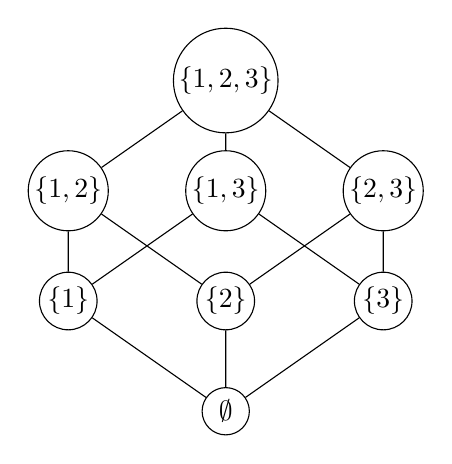
\begin{tikzpicture}[node distance=1.4cm, every node/.style={draw,circle,inner sep=1pt,minimum size=6mm}]
\node (e) at (0,0) {$\emptyset$};
\node (1) at (-2,1.4) {$\{1\}$};
\node (2) at (0,1.4) {$\{2\}$};
\node (3) at (2,1.4) {$\{3\}$};
\node (12) at (-2,2.8) {$\{1,2\}$};
\node (13) at (0,2.8) {$\{1,3\}$};
\node (23) at (2,2.8) {$\{2,3\}$};
\node (123) at (0,4.2) {$\{1,2,3\}$};
\draw (e)--(1) (e)--(2) (e)--(3);
\draw (1)--(12) (2)--(12) (1)--(13) (3)--(13) (2)--(23) (3)--(23);
\draw (12)--(123) (13)--(123) (23)--(123);
\end{tikzpicture}
\end{center}
\begin{center}
\small Hasse diagram of $(\mathcal P(\{1,2,3\}),\subseteq)$
\end{center}

\begin{definition}[Upper/lower bound, LUB, GLB -- harder]
For $S\subseteq A$: $u\in A$ is an \emph{upper bound} of $S$ if $s\preceq u$ for all $s\in S$; a \emph{least upper bound} (LUB, or \emph{join} $\vee$) is an upper bound $\preceq$ every other upper bound. Dually for \emph{lower bound} and \emph{greatest lower bound} (GLB, \emph{meet} $\wedge$).
\end{definition}

\begin{definition}[Lattice]
A poset in which every pair $a,b$ has both a LUB and a GLB.
\end{definition}

\begin{example}
$(\mathcal P(S),\subseteq)$ is a lattice: $A\vee B = A\cup B$, $A\wedge B = A\cap B$ (\S\ref{sec:1-12}).
\end{example}

\begin{note}
$(\Z^+,\mid)$ is also a lattice: $\vee = \mathrm{lcm}$, $\wedge=\gcd$.
\end{note}

\subsection{Relations}
\label{sec:2-17}
% CN 2.17 / Rosen 9.2

\begin{definition}[Ternary relation]
A \emph{ternary relation} on sets $A,B,C$ is a subset of $A \times B \times C$: a set of triples $(x,y,z)$ with $x\in A,\ y\in B,\ z\in C$.
\end{definition}

\begin{definition}[$n$-ary relation]
An \emph{$n$-ary relation} on sets $A_1,A_2,\dots,A_n$ is a subset
\[
R \subseteq A_1 \times A_2 \times \cdots \times A_n,
\]
i.e.\ a set of $n$-tuples $(x_1,\dots,x_n)$ with $x_i \in A_i$ for each $i$. Each $A_i$ is the $i$-th \emph{domain}; $n$ is the \emph{degree}. An $n$-ary relation is also called an \emph{$n$-ary predicate}.
\end{definition}

\begin{example}
$(\text{first name}, \text{middle name}, \text{surname})$ triples form a ternary relation. $(\text{day},\text{month},\text{year})$ likewise. Points in $\R^3$ form a ternary relation on $\R$.
\end{example}

\begin{note}[Connection to tables and databases, Rosen]
An $n$-ary relation's tuples correspond to the \emph{rows} of an $n$-column table; each domain $A_i$ (analogous to a function's codomain -- allowed to contain more than what actually appears) corresponds to a \emph{column} or \emph{attribute}. This correspondence is the basis of \emph{relational databases}: a database table \emph{is} an $n$-ary relation, its columns are attributes, and a \emph{key} (or combination of attributes forming a key) is one that uniquely determines each tuple -- analogous to how, in a binary relation that happens to be a function, the first coordinate uniquely determines the second.
\end{note}

\begin{definition}[Database, Rosen \S9.2.2]
A \emph{database} is (in this model) an $n$-ary relation, its tuples called \emph{records}, its domains $A_1,\dots,A_n$ called \emph{fields} or \emph{attributes}. A \emph{primary key} is a domain (or combination of domains) whose value(s) uniquely determine each record -- i.e.\ no two distinct tuples agree on it.
\end{definition}

\begin{definition}[Selection operator, Rosen \S9.2.3]
For an $n$-ary relation $R$ and a condition $C$ on $n$-tuples, the \emph{selection operator} $s_C$ maps $R$ to
\[
s_C(R) = \{(a_1,\dots,a_n) \in R : C(a_1,\dots,a_n) \text{ holds}\}.
\]
(Rows satisfying the condition -- SQL's \texttt{WHERE}.)
\end{definition}

\begin{definition}[Projection, Rosen \S9.2.3]
For $1 \le i_1 < i_2 < \cdots < i_m \le n$, the \emph{projection} $P_{i_1,\dots,i_m}$ maps each $n$-tuple to the $m$-tuple of its selected components:
\[
P_{i_1,\dots,i_m}(a_1,\dots,a_n) = (a_{i_1}, a_{i_2}, \dots, a_{i_m}).
\]
(Columns kept, duplicates then removed -- SQL's \texttt{SELECT}, confusingly named the opposite of the relational-algebra term.)
\end{definition}

\begin{note}
Projection can reduce the number of tuples: distinct $n$-tuples that agree on all $m$ retained components collapse to one $m$-tuple.
\end{note}

\begin{definition}[Join, Rosen \S9.2.3]
Let $R$ have degree $m$, $S$ have degree $n$, and fix $p \le m,n$. The \emph{join} $J_p(R,S)$ is the relation of degree $m+n-p$ consisting of all $(m+n-p)$-tuples
\[
(a_1,\dots,a_{m-p},\ c_1,\dots,c_p,\ b_1,\dots,b_{n-p})
\]
such that $(a_1,\dots,a_{m-p},c_1,\dots,c_p) \in R$ and $(c_1,\dots,c_p,b_1,\dots,b_{n-p}) \in S$ -- i.e.\ tuples of $R$ and $S$ are merged wherever their last $p$ / first $p$ components agree.
\end{definition}

\begin{note}[Applications, Rosen \S9.2.4]
$n$-ary relations underlie \emph{data mining}: a store's transaction database (each transaction an $n$-ary tuple of purchased items) can be queried with selection/projection/join to find frequent itemsets, association rules, etc.
\end{note}

\subsection{Counting relations}
\label{sec:2-18}
% CN 2.18 / Rosen (exercises, \S9.1)

\begin{theorem}[Counting binary relations]
For finite $A,B$ with $|A|=m,\ |B|=n$:
\[
\#\{\text{binary relations from } A \text{ to } B\} = 2^{mn}.
\]
In particular, with $A=B$, $|A|=m$:
\[
\#\{\text{binary relations on } A\} = 2^{m^2}.
\]
\end{theorem}
\begin{proof}
A binary relation from $A$ to $B$ is exactly a subset of $A \times B$, so the count equals $|\mathcal{P}(A\times B)| = 2^{|A\times B|}$ (\S\ref{sec:1-9}). Since $|A\times B| = mn$ (\S\ref{sec:1-14}), this is $2^{mn}$. The case $A=B$ substitutes $n=m$.
\end{proof}

\begin{theorem}[Counting $n$-ary relations]
For finite $A_1,\dots,A_n$ with $|A_i|=m_i$:
\[
\#\{n\text{-ary relations on } A_1,\dots,A_n\} = 2^{m_1 m_2 \cdots m_n}.
\]
If all $A_i = A$ with $|A|=m$: $2^{m^n}$.
\end{theorem}
\begin{proof}
Identical argument: an $n$-ary relation is a subset of $A_1\times\cdots\times A_n$, of size $\prod_i m_i$ (\S\ref{sec:1-14} generalized), so the count is $2^{\prod_i m_i}$.
\end{proof}

\begin{example}[Counting relations with a given property, Rosen-style]
Reflexive relations on $A$ with $|A|=m$: the $m$ diagonal pairs $(a,a)$ are forced \emph{in}, leaving $m^2 - m$ off-diagonal pairs free to choose independently, so there are $2^{m^2-m}$ reflexive relations on $A$.
\end{example}

\subsection{Matrices (Rosen \S\ref{sec:2-6} -- extension, beyond CN syllabus)}

\begin{definition}[Matrix]
An $m\times n$ matrix $A=[a_{ij}]$ is a rectangular array with $m$ rows, $n$ columns, entries $a_{ij}$ ($1\le i\le m,\ 1\le j\le n$). $A$ is \emph{square} if $m=n$.
\end{definition}

\begin{definition}[Addition, scalar multiplication]
For same-size $A,B$:
\[
(A+B)_{ij}=a_{ij}+b_{ij}.
\]
For scalar $c$:
\[
(cA)_{ij}=c\,a_{ij}.
\]
Addition is defined only when $A,B$ have identical dimensions.
\end{definition}

\bigskip
\begin{definition}[Matrix multiplication]
For $A$ ($m\times k$) and $B$ ($k\times n$), the product $AB$ is $m\times n$, with entry $(i,j)$ given by
\[
(AB)_{ij} = a_{i1}b_{1j} + a_{i2}b_{2j} + \cdots + a_{ik}b_{kj} = \sum_{l=1}^{k} a_{il}b_{lj}
\]
-- the dot product of row $i$ of $A$ with column $j$ of $B$. Defined only when the number of columns of $A$ equals the number of rows of $B$.
\end{definition}

\begin{example}
\[
\begin{pmatrix}1&2\\3&4\end{pmatrix}
\begin{pmatrix}5&6\\7&8\end{pmatrix}
=
\begin{pmatrix}1\cdot5+2\cdot7 & 1\cdot6+2\cdot8\\ 3\cdot5+4\cdot7 & 3\cdot6+4\cdot8\end{pmatrix}
=
\begin{pmatrix}19&22\\43&50\end{pmatrix}.
\]
\end{example}

\begin{theorem}
Matrix multiplication is associative: $(AB)C = A(BC)$ whenever the products are defined.
\end{theorem}
\begin{proof}
Let $A$ be $m\times k$, $B$ be $k\times l$, $C$ be $l\times n$. Both $(AB)C$ and $A(BC)$ are $m\times n$.

For entry $(i,j)$ of $(AB)C$: first $(AB)_{ip} = a_{i1}b_{1p}+\cdots+a_{ik}b_{kp}$ for each $p$, then
\[
\big((AB)C\big)_{ij} = \sum_{p=1}^{l} (AB)_{ip}\, c_{pj} = \sum_{p=1}^{l}\left(\sum_{q=1}^{k} a_{iq}b_{qp}\right)c_{pj} = \sum_{q=1}^{k}\sum_{p=1}^{l} a_{iq}b_{qp}c_{pj}.
\]

For entry $(i,j)$ of $A(BC)$: first $(BC)_{qj} = b_{q1}c_{1j}+\cdots+b_{ql}c_{lj}$ for each $q$, then
\[
\big(A(BC)\big)_{ij} = \sum_{q=1}^{k} a_{iq}\,(BC)_{qj} = \sum_{q=1}^{k} a_{iq}\left(\sum_{p=1}^{l} b_{qp}c_{pj}\right) = \sum_{q=1}^{k}\sum_{p=1}^{l} a_{iq}b_{qp}c_{pj}.
\]

Both expand to the same triple sum $\sum_{q,p} a_{iq}b_{qp}c_{pj}$ (finite sums may be freely reordered/regrouped), so $(AB)C=A(BC)$.
\end{proof}

\begin{theorem}
Matrix multiplication is \emph{not} commutative in general.
\end{theorem}
\begin{proof}
\[
\begin{pmatrix}1&1\\0&0\end{pmatrix}\begin{pmatrix}1&0\\1&0\end{pmatrix} = \begin{pmatrix}2&0\\0&0\end{pmatrix}, \qquad
\begin{pmatrix}1&0\\1&0\end{pmatrix}\begin{pmatrix}1&1\\0&0\end{pmatrix} = \begin{pmatrix}1&1\\1&1\end{pmatrix}.
\]
Different results, so $AB\neq BA$ here.
\end{proof}

\bigskip
\begin{definition}[Identity matrix]
$I_n$ is $n\times n$ with $1$s on the diagonal, $0$s elsewhere: $(I_n)_{ij} = 1$ if $i=j$, else $0$.
\end{definition}

\begin{theorem}
For $A$ ($m\times n$): $I_mA=A$ and $AI_n=A$.
\end{theorem}

\begin{definition}[Transpose]
$A^t$: $(A^t)_{ij}=a_{ji}$ -- rows and columns swapped.
\end{definition}

\begin{theorem}
$(A+B)^t = A^t+B^t$; $(AB)^t = B^tA^t$ (order reverses).
\end{theorem}

\begin{definition}[Symmetric matrix]
$A$ is \emph{symmetric} if $A=A^t$ (equivalently $a_{ij}=a_{ji}$ for all $i,j$; requires $A$ square).
\end{definition}

\bigskip
\begin{definition}[Zero-one matrices, meet/join/Boolean product, Rosen -- harder, sets up \S\ref{sec:2-15}/9.4]
For matrices with entries in $\{0,1\}$:
\[
(A\wedge B)_{ij}=a_{ij}\wedge b_{ij} \quad \text{(meet)}, \qquad (A\vee B)_{ij}=a_{ij}\vee b_{ij} \quad \text{(join)}.
\]
Boolean product:
\[
(A\odot B)_{ij} = (a_{i1}\wedge b_{1j}) \vee (a_{i2}\wedge b_{2j}) \vee \cdots \vee (a_{ik}\wedge b_{kj}) = \bigvee_{l=1}^{k} (a_{il}\wedge b_{lj}).
\]
An entry is $1$ iff \emph{some} $l$ has $a_{il}=b_{lj}=1$ -- same shape as ordinary matrix multiplication with $(\vee,\wedge)$ in place of $(+,\times)$.
\end{definition}

\begin{example}
\[
A=\begin{pmatrix}1&0\\1&1\end{pmatrix}, \quad B=\begin{pmatrix}0&1\\1&0\end{pmatrix}.
\]
\[
A\wedge B = \begin{pmatrix}0&0\\1&0\end{pmatrix}, \qquad A\vee B = \begin{pmatrix}1&1\\1&1\end{pmatrix}, \qquad A\odot B = \begin{pmatrix}0&1\\1&1\end{pmatrix}.
\]
For $(A\odot B)_{11}$: $(a_{11}\wedge b_{11})\vee(a_{12}\wedge b_{21}) = (1\wedge0)\vee(0\wedge1)=0$. For $(A\odot B)_{21}$: $(1\wedge0)\vee(1\wedge1)=1$.
\end{example}

\begin{theorem}[Connection to relations, Rosen]
Let $A$ be the zero-one matrix of relation $R\subseteq X\times Y$ (\S\ref{sec:2-13}: $a_{ij}=1\iff(x_i,y_j)\in R$), $B$ that of $S\subseteq Y\times Z$. Then $A\odot B$ is exactly the matrix of $S\circ R$ (\S\ref{sec:2-15}).
\end{theorem}
\begin{proof}
\[
(A\odot B)_{ij}=1 \iff \exists l:\ a_{il}=1 \wedge b_{lj}=1 \iff \exists y_l:\ (x_i,y_l)\in R \wedge (y_l,z_j)\in S \iff (x_i,z_j)\in S\circ R,
\]
matching the definition of relation composition exactly (\S\ref{sec:2-15}).
\end{proof}

\begin{note}[Iterating for closures]
Writing $A^{[n]} = A\odot A\odot\cdots\odot A$ ($n$ copies) gives the matrix of $R^{(n)}$. For finite $A$ ($n\times n$ zero-one matrix), the join $A\vee A^{[2]}\vee\cdots\vee A^{[n]}$ (only $n$ terms needed, since further terms add nothing new) gives the matrix of the transitive closure $R^+$ (\S\ref{sec:2-15}) -- this is the basis of \emph{Warshall's algorithm}, computed far more efficiently than by literally forming all powers.
\end{note}

% ============================================================
% CHAPTER 3 --- PROOFS  (CN Ch.3, §3.1-3.15)
% ============================================================
\newpage
\section{Proofs}

\subsection{Theorems and proofs}
\label{sec:3-1}
% CN 3.1 / Rosen 1.7

\begin{definition}[Theorem]
A \emph{theorem} is a mathematical statement that has been proved true.
\end{definition}

\begin{definition}[Lemma, proposition, corollary -- Rosen's terminology]
A \emph{lemma} is a theorem whose main purpose is as a stepping stone in the proof of a more significant theorem. A \emph{proposition} is a theorem of independent interest, typically less significant or easier to prove than the main theorems around it. A \emph{corollary} is a theorem that follows almost immediately from one just proved.
\end{definition}

\begin{definition}[Proof]
A \emph{proof} of a claim is a finite sequence of statements (\emph{steps}), ending in the claim, where each step is one of:
\begin{itemize}
    \item something already known: a \emph{definition}, an \emph{axiom} (a fundamental assumed property, e.g.\ $x(y+z)=xy+xz$), or a previously proved theorem;
    \item an \emph{assumption}, made as a starting point;
    \item a \emph{logical consequence} of earlier steps.
\end{itemize}
The final step establishes the claim from what precedes it.
\end{definition}

\begin{note}[Verifiability]
A proof must be readable sequentially -- each step justified only by what comes \emph{before} it, never by reading ahead. The end of a proof is marked by $\blacksquare$ (or historically ``Q.E.D.'', \emph{quod erat demonstrandum}).
\end{note}

\begin{theorem}
For any sets $A, B$: if $A \subseteq B$ then $\mathcal{P}(A) \subseteq \mathcal{P}(B)$.
\end{theorem}
\begin{proof}
Assume $A \subseteq B$. Let $X \in \mathcal{P}(A)$; then $X \subseteq A$ by definition of $\mathcal{P}(A)$. Since $A \subseteq B$, also $X \subseteq B$. Hence $X \in \mathcal{P}(B)$ by definition of $\mathcal{P}(B)$. So $X \in \mathcal{P}(A) \implies X \in \mathcal{P}(B)$, i.e.\ $\mathcal{P}(A) \subseteq \mathcal{P}(B)$.
\end{proof}

\begin{note}[Annotating each step]
\begin{itemize}
    \item ``Assume $A\subseteq B$'' -- an \emph{assumption} (the theorem is conditional on it).
    \item ``Let $X \in \mathcal{P}(A)$'' -- a \emph{definition}, naming an arbitrary element so we can reason about it generically.
    \item ``$X \subseteq A$'' -- a \emph{logical consequence} of the previous line and the definition of $\mathcal{P}(A)$.
    \item ``$X \subseteq B$'' -- a consequence of $X\subseteq A$ and the assumption $A \subseteq B$.
    \item ``$X \in \mathcal{P}(B)$'' -- a consequence of $X \subseteq B$ and the definition of $\mathcal{P}(B)$.
    \item Final line -- restates the whole chain as the subset relation $\mathcal{P}(A)\subseteq\mathcal{P}(B)$.
\end{itemize}
Every line either restates a definition/axiom, states an assumption, or follows logically from what came strictly before -- exactly the requirement above.
\end{note}

\subsection{Logical deduction}
\label{sec:3-2}
% CN 3.2 / Rosen 1.6-1.7

\begin{note}[Modus ponens]
The core deduction rule: if $P$ has been established, and $P \implies Q$ has been established, then $Q$ may be deduced. This is used constantly and rarely named explicitly, but it is the essence of every logical deduction step in a proof.
\end{note}

\begin{note}[Implication as a subset relation]
In general, for statements $P,Q$, let $\hat P, \hat Q$ be the sets of situations in which $P$, resp.\ $Q$, holds. Then
\[
P \implies Q \quad \text{corresponds to} \quad \hat P \subseteq \hat Q.
\]
This generalizes the set-membership fact from \S\ref{sec:1-6}: $A \subseteq B \iff \forall x\,(x\in A \implies x \in B)$ -- the correspondence holds even when $P,Q$ are not phrased as membership statements at all (as the domino example shows).
\end{note}

\begin{note}[Vacuous truth]
If $X$ is false, $X \implies Y$ is true regardless of $Y$ -- corresponding to $\emptyset \subseteq Y$ for any set $Y$ (\S\ref{sec:1-6}, Theorem 1: the empty set is a subset of every set).
\end{note}

\begin{definition}[Converse]
The \emph{converse} of $P \implies Q$ is $Q \implies P$ (equivalently written $P \impliedby Q$). An implication holding does \emph{not} entail its converse holds: implication is not symmetric, as both examples above show ($P\Rightarrow Q$ but not $Q \Rightarrow P$; $X \Rightarrow Y$ but not $Y \Rightarrow X$).
\end{definition}

\begin{definition}[Biconditional]
When both $P \implies Q$ and its converse $Q \implies P$ hold, we write $P \iff Q$ (``$P$ if and only if $Q$''; $P,Q$ are \emph{logically equivalent}: $\hat P = \hat Q$ as sets of situations).
\end{definition}

\begin{definition}[Contrapositive and inverse, Rosen]
For $P \implies Q$: the \emph{contrapositive} is $\neg Q \implies \neg P$; the \emph{inverse} is $\neg P \implies \neg Q$.
\end{definition}

\begin{theorem}
$P \implies Q$ is logically equivalent to its contrapositive $\neg Q \implies \neg P$. It is \emph{not}, in general, equivalent to its converse or its inverse (which are themselves contrapositives of each other).
\end{theorem}
\begin{proof}
Both $P\Rightarrow Q$ and $\neg Q \Rightarrow \neg P$ are false in exactly one case ($P$ true, $Q$ false) and true otherwise -- identical truth tables, hence logically equivalent. The converse $Q\Rightarrow P$ and inverse $\neg P \Rightarrow \neg Q$ each fail in the case $P$ false, $Q$ true (for the converse) or $P$ false, $Q$ true (checking directly) -- a different failure case from the original, so neither need agree with $P \Rightarrow Q$ in general; the domino example ($P\Rightarrow Q$ true, $Q \Rightarrow P$ false) is a concrete witness.
\end{proof}

\begin{note}[Common logical fallacies, Rosen]
\emph{Affirming the consequent}: from $P\implies Q$ and $Q$, wrongly concluding $P$ (this is the \emph{converse} error from earlier in this section). \emph{Denying the antecedent}: from $P\implies Q$ and $\neg P$, wrongly concluding $\neg Q$ (this is the \emph{inverse} error). \emph{Begging the question / circular reasoning}: using the claim being proved (or something equivalent to it) as a premise in its own proof.
\end{note}

\begin{example}[Affirming the consequent, in the wild]
``If it rains, the ground is wet. The ground is wet. Therefore it rained.'' Invalid: the ground could be wet from a sprinkler.
\end{example}

\subsection{Proofs of existential and universal statements}
\label{sec:3-3}
% CN 3.3 / Rosen 1.4, 1.7

\begin{definition}[Existential statement]
An \emph{existential statement} asserts $\exists x \in D,\ P(x)$ for some domain $D$ and predicate $P$: that \emph{something} with the stated property exists. It may be true or false.
\end{definition}

\begin{theorem}
English has a palindrome.
\end{theorem}
\begin{proof}
`rotator' is an English word, and it reads the same forwards and backwards.
\end{proof}

\begin{note}[Proving $\exists x,\ P(x)$]
A single \emph{witness} suffices: exhibit one $x \in D$ and verify $P(x)$ holds. No need to search further once found.
\end{note}

\begin{definition}[Universal statement]
A \emph{universal statement} asserts $\forall x \in D,\ P(x)$: \emph{everything} in $D$ has the property.
\end{definition}

\begin{theorem}
Every English word has a vowel or a `y'.
\end{theorem}
\begin{proof}[Proof sketch]
One could, in principle, check every English word individually (`aardvark' has a vowel; `aardwolf' has a vowel; \dots; `syzygy' has a `y'; \dots) -- but $D$ here has tens of thousands of members, making case-by-case verification impractical (and hopeless for an infinite $D$).
\end{proof}

\begin{note}[Proving $\forall x \in D,\ P(x)$]
Checking every case individually only works for small, finite $D$ -- and not even then, practically. Instead: let $x$ be an \emph{arbitrary, generic} element of $D$ (no properties assumed beyond $x \in D$), and show $P(x)$ follows from that alone. Since the argument uses nothing specific to the particular $x$ chosen, it applies to \emph{every} element of $D$ simultaneously. This is the technique already used, e.g., in \S\ref{sec:1-6} (``let $x \in A$, show $x \in B$'') and in \S\ref{sec:3-1}'s Theorem 13 proof (``let $X \in \mathcal{P}(A)$'').
\end{note}

\begin{note}[Disproof is the mirror image]
To \emph{disprove} a universal statement $\forall x \in D,\ P(x)$ (i.e.\ prove its negation $\exists x \in D,\ \neg P(x)$), a single \emph{counterexample} suffices -- disproof of a universal is existential proof of its negation. Conversely, disproving an existential statement $\exists x \in D,\ P(x)$ requires proving the universal $\forall x \in D,\ \neg P(x)$ -- generally the harder direction, since no single case can rule out all possibilities.
\end{note}

\begin{theorem}[Uniqueness example]
There is exactly one real number $x$ such that $2x+3=7$.
\end{theorem}
\begin{proof}
\textbf{Existence}: $x=2$ satisfies $2(2)+3=7$.

\textbf{Uniqueness}: suppose $x_1,x_2$ both satisfy $2x+3=7$. Then $2x_1+3=2x_2+3$, so $2x_1=2x_2$, so $x_1=x_2$.

So exactly one such $x$ exists.
\end{proof}

\begin{note}[The uniqueness pattern]
Assume two witnesses $x_1,x_2$ both satisfy the property; derive $x_1=x_2$. Combined with a separate existence argument, this proves ``exactly one.''
\end{note}

\begin{example}[A plausible-looking false universal claim]
Claim: ``every prime $p$ satisfies $2^p-1$ is prime'' (a \emph{Mersenne prime} for every prime exponent).
\end{example}
\begin{proof}[Disproof by counterexample]
$p=11$ is prime, but $2^{11}-1 = 2047 = 23\times89$, not prime. So the universal claim is false -- a single counterexample suffices, despite the pattern holding for $p=2,3,5,7$ ($2^p-1=3,7,31,127$, all prime).
\end{proof}

\begin{note}
This is a genuine cautionary example: checking several small cases can be misleading. $p=2,3,5,7$ all work, and it's tempting to conjecture the pattern continues -- but $p=11$ already breaks it.
\end{note}

\subsection{Finding proofs}
\label{sec:3-4}
% CN 3.4 / Rosen 1.7-1.8

\begin{note}[No algorithm for finding proofs]
There is no systematic method for discovering proofs, for deep theoretical reasons (Gödel 1931, Church 1936, Turing 1936). Finding proofs draws on logical reasoning, familiarity with the objects involved, practice, creativity, and persistence -- not a fixed recipe.
\end{note}

\begin{note}[Strategy: proving $A \subseteq B$]
\begin{enumerate}[label=\arabic*.]
    \item Name a general member: ``Let $x \in A$.''
    \item Unpack what the definition of $A$ tells you about $x$.
    \item Follow the logical consequences.
    \item Aim to conclude $x$ satisfies the definition of $B$.
\end{enumerate}
\end{note}

\begin{note}[Strategy: proving $A = B$ (sets)]
Prove $A \subseteq B$ and $A \supseteq B$ separately (\S\ref{sec:1-6}). Each direction uses the subset strategy above.
\end{note}

\begin{note}[Strategy: proving $A = B$ (numbers)]
If direct symbolic manipulation (algebraic rules) can transform expression $A$ into expression $B$, use that. Otherwise, prove $A \le B$ and $A \ge B$ separately -- the numerical analogue of the double-inclusion technique.
\end{note}

\begin{note}[Without loss of generality (WLOG), Rosen]
When a proof is symmetric in two variables (swapping them leaves the claim unchanged), it suffices to prove one case and invoke the symmetry for the other -- written ``WLOG, assume $x\le y$'' etc. Using WLOG when the situation is \emph{not} actually symmetric is a common error -- check the symmetry claim carefully before invoking it.
\end{note}

\begin{note}[Forward vs.\ backward reasoning, Rosen]
\emph{Forward}: start from known facts/assumptions, derive consequences, until reaching the goal. \emph{Backward}: start from the goal, ask ``what would suffice to prove this?'', and work backward to something already known. Backward reasoning is often how a proof is \emph{discovered}; it is then usually rewritten forward for presentation.
\end{note}

\subsection{Types of proofs}
\label{sec:3-5}
% CN 3.5 / Rosen 1.7-1.8

\begin{note}[Proof types]
\begin{itemize}
    \item \emph{Direct proof / proof by symbolic manipulation} (\S\ref{sec:3-6}): assume $P$, derive $Q$ via a direct chain of implications or equations.
    \item \emph{Proof by construction} (\S\ref{sec:3-7}, also called \emph{proof by example}): exhibit a specific object and verify it works -- a \emph{constructive} existence proof, producing an explicit witness (contrast: \emph{nonconstructive} existence proofs establish that something exists, e.g.\ via contradiction or a counting argument, without exhibiting it).
    \item \emph{Proof by cases} (\S\ref{sec:3-8}): split the domain into exhaustive cases, prove the claim in each.
    \item \emph{Proof by contradiction} (\S\ref{sec:3-9}): assume the negation of the claim, derive a contradiction (some statement and its negation both true).
    \item \emph{Proof by contraposition}: to prove $P \implies Q$, instead prove the equivalent $\neg Q \implies \neg P$ (\S\ref{sec:3-2}'s contrapositive theorem) -- useful when $\neg Q$ gives more to work with than $P$ does.
    \item \emph{Vacuous / trivial proof}: prove $P \implies Q$ by showing $P$ is always false (vacuous) or $Q$ is always true (trivial).
    \item \emph{Proof by (mathematical) induction} (\S\ref{sec:3-10}).
    \item \emph{Uniqueness proofs}: show existence, then show any two witnesses must coincide.
\end{itemize}
This list is not exhaustive, and real proofs frequently mix several of these -- e.g.\ a proof by cases where one case is handled by contradiction and another by direct construction.
\end{note}

\begin{example}[Vacuous proof]
``For all $x\in\emptyset$, $x^2<0$.'' True vacuously: $\emptyset$ has no members, so the implication ``$x\in\emptyset \implies x^2<0$'' is never tested against an actual counterexample.
\end{example}

\begin{example}[Trivial proof]
``If $n>0$, then $n^2+1>0$.'' The conclusion $n^2+1>0$ holds for \emph{every} real $n$ regardless of the hypothesis, so the implication is trivially true.
\end{example}

\bigskip
\begin{theorem}[Contraposition example]
If $n^2$ is even, then $n$ is even.
\end{theorem}
\begin{proof}[Proof by contraposition]
We prove the contrapositive: if $n$ is odd, then $n^2$ is odd. Suppose $n=2k+1$ for some $k\in\Z$. Then
\[
n^2 = (2k+1)^2 = 4k^2+4k+1 = 2(2k^2+2k)+1,
\]
which is odd. By \S\ref{sec:3-2}'s contrapositive theorem, this proves the original statement.
\end{proof}

\begin{note}
Contraposition was the right tool here because ``$n$ is odd'' gives a concrete algebraic form ($2k+1$) to compute with, while ``$n^2$ is even'' does not directly hand you a useful form for $n$ itself.
\end{note}

\subsection{Proof by symbolic manipulation}
\label{sec:3-6}
% CN 3.6 / Rosen (equational reasoning, throughout Ch.1-2)

\begin{note}[The pattern]
A chain of equations, each step justified by a known law (axiom or previously proved fact), linking the two sides of the claim.
\end{note}

\begin{theorem}[Difference of two squares]
\[
(x-y)(x+y) = x^2 - y^2.
\]
\end{theorem}
\begin{proof}
\begin{align*}
(x-y)(x+y) &= x^2 + xy - yx - y^2 && \text{(distributive law)} \\
&= x^2 + xy - xy - y^2 && \text{(commutativity of multiplication)} \\
&= x^2 - y^2 && \text{(additive cancellation)}.
\end{align*}
\end{proof}

\begin{note}[Direction is arbitrary]
The proof above started from the \emph{right}-hand side and worked toward the left -- equally valid as starting from the left. Pick whichever direction is more natural for the specific identity.
\end{note}

\begin{note}[Examples already seen in this note]
This is exactly the technique behind: the De Morgan's-law proof via set-builder notation (\S\ref{sec:1-11}), the chained-identity proof $\overline{A\cup(B\cap C)} = (\overline{C}\cup\overline{B})\cap\overline{A}$ (\S\ref{sec:1-11}), and the symmetric-difference identities $A\triangle B = \overline{A\triangle B}$ etc.\ (\S\ref{sec:1-13}) -- each is a sequence of equalities, each step citing a specific law.
\end{note}

\subsection{Proof by construction}
\label{sec:3-7}
% CN 3.7 / Rosen: constructive existence proof
\begin{note}[Pattern]
Describe a specific object precisely, and show it exists and satisfies the required conditions -- a \emph{constructive} proof of an existential statement (\S\ref{sec:3-3}). Theorem 14 (`rotator' is a palindrome) is an example.
\end{note}

\begin{note}[Two mistakes to avoid]
\begin{itemize}
    \item Using construction to attempt a \emph{universal} statement: exhibiting one object with a property never establishes that \emph{every} object has it.
    \item Mistaking an illustrative example for a proof: an example can clarify a proof's ideas, but is not itself a proof unless the statement being proved is genuinely existential.
\end{itemize}
\end{note}

\begin{theorem}[Ramanujan's taxicab number, Rosen]
There is a positive integer expressible as the sum of two positive cubes in two genuinely different ways.
\end{theorem}
\begin{proof}
\[
1729 = 10^3 + 9^3 = 1000 + 729 = 12^3 + 1^3 = 1728 + 1.
\]
Both decompositions use positive integers, and $\{10,9\} \neq \{12,1\}$, so these are two different ways.
\end{proof}

\begin{note}
This is the smallest such number -- hence its fame as the ``taxicab number,'' from the (possibly apocryphal) anecdote of Hardy visiting Ramanujan in a taxi numbered 1729.
\end{note}

\subsection{Proof by cases}
\label{sec:3-8}
% CN 3.8 / Rosen: proof by cases / exhaustive proof
\begin{note}[Pattern]
Identify finitely many cases covering every possibility, and prove the theorem separately in each -- each case-proof is a subproof. Cases may overlap (though this can signal redundant effort), but together they must be \emph{exhaustive}: every object the theorem concerns must fall into at least one case.
\end{note}

\begin{note}[Typical shape]
Often a theorem concerns an \emph{infinite} set, split into a small number of cases, at least one of which still covers infinitely many objects -- the reasoning within that case must be general enough to apply to all of them, not just verify a few instances.
\end{note}

\begin{theorem}[Nonconstructive existence via cases, Rosen]
There exist irrational numbers $x, y$ such that $x^y$ is rational.
\end{theorem}
\begin{proof}
Consider $\sqrt{2}^{\sqrt{2}}$. Either it is rational or it is irrational -- these are the only two (exhaustive) cases.

\textbf{Case 1: $\sqrt{2}^{\sqrt{2}}$ is rational.} Take $x = y = \sqrt{2}$, both irrational, with $x^y$ rational by assumption. Done.

\textbf{Case 2: $\sqrt{2}^{\sqrt{2}}$ is irrational.} Take $x = \sqrt{2}^{\sqrt{2}}$ (irrational, by this case's assumption) and $y = \sqrt{2}$ (irrational). Then
\[
x^y = \left(\sqrt{2}^{\sqrt{2}}\right)^{\sqrt{2}} = \sqrt{2}^{\sqrt{2}\cdot\sqrt{2}} = \sqrt{2}^2 = 2,
\]
which is rational. Done.

Either way, such $x,y$ exist.
\end{proof}

\begin{note}[Strikingly nonconstructive]
This proves the statement true \emph{without ever determining which case actually holds} -- we don't know, from this proof alone, whether $\sqrt2^{\sqrt2}$ itself is rational or irrational. (It is, in fact, irrational -- even transcendental, by the Gelfond--Schneider theorem -- but that fact is not needed here.) This is the clearest illustration of the constructive/nonconstructive distinction from \S\ref{sec:3-5}.
\end{note}

\bigskip
\begin{definition}[Chomp]
A rectangular grid of cookies; players alternate taking a cookie and every cookie above-and-to-the-right of it (relative to a fixed corner); the top-left cookie is poisoned; whoever takes it loses.
\end{definition}

\begin{example}[Chomp -- Rosen \S\ref{sec:1-8}, nonconstructive existence via strategy-stealing]
On any rectangular Chomp board with more than one cookie, the \emph{first} player has a winning strategy.
\end{example}
\begin{proof}
Consider the first player's opening move: take just the bottom-right cookie.

\textbf{Case 1}: this opening move is part of \emph{some} winning strategy for the first player. Then the first player has a winning strategy -- done.

\textbf{Case 2}: this opening move is \emph{not} part of any winning strategy for the first player. Then the second player, facing the resulting position, must have a winning response $r$. But now imagine the first player had opened with exactly that move $r$ instead (a legal first move, since it was a legal move for the second player from a position that only has more cookies removed than the empty-except-poison start). By the same argument, whatever position $r$ leads to, the first player is now in the position the second player would have been in Case 2 -- with a winning strategy available.

Either way, the first player wins.
\end{proof}

\begin{note}[Why this is nonconstructive]
The proof establishes a winning strategy \emph{exists} for the first player without ever revealing what it is -- indeed, for most board sizes, no explicit winning strategy is known at all. This is the sharpest possible illustration of the constructive/nonconstructive distinction (\S\ref{sec:3-5}): the theorem is proved, but the object it asserts exists (the strategy) remains, in general, unknown.
\end{note}

\begin{note}[Strategy-stealing, the technique]
The argument never analyzes what the winning strategy actually \emph{does} -- it only argues that \emph{if} the second player had a winning response, the first player could ``steal'' it by playing that same move first. This strategy-stealing pattern appears throughout combinatorial game theory whenever a game has the property that having extra pieces on the board never hurts a player (true for Chomp, since eaten cookies only shrink future options for both sides equally).
\end{note}

\subsection{Proof by contradiction}
\label{sec:3-9}
% CN 3.9 / Rosen 1.7-1.8 (proof by contradiction, reductio ad absurdum)
\begin{note}[Pattern]
Assume the \emph{negation} of the claim; reason from it to a contradiction (some statement and its negation both derived as true); conclude the assumption was false, so the original claim holds.
\end{note}

\begin{theorem}[Euclid]
There are infinitely many prime numbers.
\end{theorem}
\begin{proof}
Suppose, for contradiction, that there are only finitely many primes $p_1,p_2,\dots,p_n$. Let
\[
q = p_1 p_2 \cdots p_n + 1.
\]
Since $q > p_i$ for every $i$, $q$ is not itself prime, so $q$ is composite and hence divisible by some prime. But for each $p_i$, dividing $q$ by $p_i$ leaves remainder $1$ (since $p_i$ divides $p_1\cdots p_n$ exactly), so $p_i \nmid q$. So $q$ is divisible by no prime at all -- contradicting that $q$ is composite. Hence the assumption was false: there are infinitely many primes.
\end{proof}

\begin{note}[A useful auxiliary fact used implicitly]
The argument above (and many proofs by contradiction over $\N$ or $\Z^+$) relies on: any nonempty set of natural numbers has a smallest element (well-ordering). This lets you say things like ``let $n$ be the smallest counterexample'' and derive a contradiction from its minimality.
\end{note}

\begin{theorem}
$\sqrt{2}$ is irrational.
\end{theorem}
\begin{proof}
Suppose, for contradiction, that $\sqrt2$ is rational: $\sqrt2 = a/b$ for integers $a,b$ with no common factor (in lowest terms). Squaring, $2 = a^2/b^2$, so $a^2 = 2b^2$ -- hence $a^2$ is even, hence $a$ is even (an odd number squares to an odd number), say $a = 2c$. Substituting: $4c^2 = 2b^2$, so $b^2 = 2c^2$ -- hence $b^2$ is even, hence $b$ is even. But then $a$ and $b$ are \emph{both} even, contradicting that $a/b$ was in lowest terms. So the assumption was false: $\sqrt2$ is irrational.
\end{proof}

\begin{note}
Alongside Euclid's proof, this is the other canonical proof-by-contradiction example in mathematics -- both hinge on deriving a property (divisibility, in each case) that eventually contradicts an assumption baked into the setup (finiteness of the prime list; lowest-terms form of the fraction).
\end{note}

\bigskip
\begin{note}[Open problems, Rosen]
Not every true mathematical statement has a known proof. An \emph{open problem} is a precisely stated claim believed true (or at least undecided) but not yet proved or disproved.
\end{note}

\begin{example}[The Collatz conjecture]
Define, for $n\in\Z^+$:
\[
\mathrm{Collatz}(n) = \begin{cases} n/2, & n \text{ even}, \\ 3n+1, & n \text{ odd}. \end{cases}
\]
\emph{Conjecture}: iterating $\mathrm{Collatz}$ from any starting $n\in\Z^+$ eventually reaches $1$.
\end{example}

\begin{note}
Verified by computer for enormous ranges of starting values, but no proof (or disproof) is known -- an active open problem since 1937. Contrast with Euclid's infinitude-of-primes proof (\S\ref{sec:3-9} above): that claim, once conjectured, was fully settled by a short contradiction argument; Collatz has resisted proof for nearly a century despite its simple statement.
\end{note}

\subsection{Proof by mathematical induction}
\label{sec:3-10}
% CN 3.10 / Rosen 5.1, 5.2

\begin{note}[Principle of mathematical induction]
To prove $S(n)$ holds for all $n \in \N$ (or all $n \ge n_0$):
\begin{itemize}
    \item \textbf{Base case}: prove $S(1)$ (or $S(n_0)$).
    \item \textbf{Inductive step}: prove, for all $k$:
    \[
    S(k) \implies S(k+1)
    \]
    (the assumption $S(k)$ here is the \emph{inductive hypothesis}).
\end{itemize}
Conclude $S(n)$ holds for all $n$.
\end{note}

\begin{note}[Why this works]
$S(1)$ holds (base case). Then:
\[
S(1) \implies S(2), \qquad S(2) \implies S(3), \qquad S(3) \implies S(4), \qquad \dots
\]
Induction packages this infinite chain of modus ponens applications into a single finite argument, rather than an informal ``and so on forever.''
\end{note}

\bigskip
\begin{theorem}[Generalized De Morgan's law, CN Thm 18]
For all $n \in \N$ and sets $A_1,\dots,A_n$:
\[
\overline{A_1 \cup A_2 \cup \cdots \cup A_n} = \overline{A_1} \cap \overline{A_2} \cap \cdots \cap \overline{A_n}.
\]
\end{theorem}
\begin{proof}
Let $S(n)$ be this identity for a given $n$.

\textbf{Base case} ($n=1$):
\[
\overline{A_1} = \overline{A_1}.
\]

\textbf{Inductive step}: assume $S(k)$, i.e.
\[
\overline{A_1\cup\cdots\cup A_k} = \overline{A_1}\cap\cdots\cap\overline{A_k}.
\]
Then
\[
\overline{A_1\cup\cdots\cup A_k \cup A_{k+1}} = \overline{(A_1\cup\cdots\cup A_k) \cup A_{k+1}} = \overline{(A_1\cup\cdots\cup A_k)} \cap \overline{A_{k+1}}
\]
by ordinary De Morgan's law (\S\ref{sec:1-11}). Applying $S(k)$ to the first factor:
\[
= (\overline{A_1}\cap\cdots\cap\overline{A_k})\cap\overline{A_{k+1}} = \overline{A_1}\cap\cdots\cap\overline{A_{k+1}},
\]
which is $S(k+1)$.

By induction, $S(n)$ holds for all $n$.
\end{proof}

\bigskip
\begin{theorem}[Divisibility example]
For all $n\in\N$: $3 \mid (n^3-n)$.
\end{theorem}
\begin{proof}
\textbf{Base case} ($n=0$): $n^3-n=0$, and $3\mid 0$.

\textbf{Inductive step}: assume $3\mid(k^3-k)$ for some $k\ge0$, i.e.\ $k^3-k=3m$ for some $m\in\Z$. Consider $n=k+1$:
\[
(k+1)^3-(k+1) = k^3+3k^2+3k+1-k-1 = (k^3-k) + 3k^2+3k = 3m+3k^2+3k = 3(m+k^2+k).
\]
This is $3$ times an integer, so $3\mid\big((k+1)^3-(k+1)\big)$.

By induction, $3\mid(n^3-n)$ for all $n\in\N$.
\end{proof}

\bigskip
\begin{definition}[Well-ordering property]
Every nonempty subset of $\N$ has a least element.
\end{definition}

\begin{theorem}[Well-ordering $\implies$ mathematical induction]
If the well-ordering property holds for $\N$, then the principle of mathematical induction is valid.
\end{theorem}
\begin{proof}
Suppose $S(1)$ holds and $S(k)\implies S(k+1)$ for all $k\ge1$. Suppose, for contradiction, $S(n)$ fails for some $n$. Let
\[
F = \{n\in\Z^+ : S(n) \text{ is false}\}.
\]
$F\neq\emptyset$ by assumption, so by well-ordering, $F$ has a least element $m$. Since $S(1)$ holds, $m\neq1$, so $m\ge2$ and $m-1\ge1$. Since $m$ is the \emph{least} element of $F$, $m-1\notin F$, i.e.\ $S(m-1)$ holds. But then the inductive step gives $S(m-1)\implies S(m)$, so $S(m)$ holds -- contradicting $m\in F$.

So $F=\emptyset$: $S(n)$ holds for all $n$.
\end{proof}

\begin{note}
This is why induction and well-ordering are often called \emph{equivalent} principles over $\N$ -- each can be used to derive the other, and most texts (Rosen included) simply take one as an axiom and prove the other as a consequence.
\end{note}

\bigskip
\begin{definition}[Principle of strong induction, formal statement]
To prove $S(n)$ for all $n\ge n_0$:
\begin{itemize}
    \item \textbf{Base case}: prove $S(n_0)$.
    \item \textbf{Inductive step}: prove, for all $k\ge n_0$: if $S(n_0),S(n_0+1),\dots,S(k)$ \emph{all} hold, then $S(k+1)$ holds.
\end{itemize}
\end{definition}

\begin{note}[Strong vs.\ weak induction -- equivalent in power]
Strong induction's hypothesis is more generous (all of $S(n_0),\dots,S(k)$, not just $S(k)$), but this doesn't let you prove anything weak induction can't -- any strong-induction proof can be mechanically rewritten as a weak-induction proof of the stronger statement $T(n) = S(n_0)\wedge\cdots\wedge S(n)$. Strong induction is a convenience, not a logically stronger tool. See \S\ref{sec:3-11} for worked examples of both.
\end{note}

\subsection{Induction: more examples}
\label{sec:3-11}
% CN 3.11 / Rosen 5.1, 5.2

\begin{theorem}[Sum of the first $n$ positive integers, CN Thm 19]
For all $n \ge 1$:
\[
1 + 2 + \cdots + n = \frac{n(n+1)}{2}.
\]
\end{theorem}
\begin{proof}
\textbf{Base case} ($n=1$): LHS $=1$, RHS $=1\cdot2/2=1$.

\textbf{Inductive step}: assume $1+\cdots+k = k(k+1)/2$ for some $k\ge1$. Then
\[
1+\cdots+k+(k+1) = \frac{k(k+1)}{2} + (k+1) = (k+1)\left(\frac{k}{2}+1\right) = \frac{(k+1)(k+2)}{2},
\]
which is the formula for $n=k+1$.

By induction, the formula holds for all $n \ge 1$.
\end{proof}

\bigskip
\begin{theorem}[$2^n > n^2$ for $n \ge 5$, Rosen -- inequality with nontrivial base]
For every integer $n \ge 5$: $2^n > n^2$.
\end{theorem}
\begin{proof}
\textbf{Base case} ($n=5$): $2^5 = 32 > 25 = 5^2$.

\textbf{Inductive step}: let $k \ge 5$, assume $2^k > k^2$. We want $2^{k+1} > (k+1)^2$.
\[
2^{k+1} = 2\cdot 2^k > 2k^2 \qquad \text{(inductive hypothesis)}.
\]
It suffices to show $2k^2 \ge (k+1)^2$ for $k \ge 5$:
\[
2k^2 - (k+1)^2 = k^2 - 2k - 1 = (k-1)^2 - 2,
\]
which is positive whenever $(k-1)^2 > 2$, i.e.\ certainly for $k \ge 5$. So $2k^2 > (k+1)^2$, hence $2^{k+1} > 2k^2 > (k+1)^2$.

By induction, $2^n > n^2$ for all $n \ge 5$.
\end{proof}

\begin{note}[Why the base case matters here]
The inequality is \emph{false} for $n=1,2,3,4$. Getting the base case right -- and matching it to where the inductive step's algebra actually works -- is essential; a careless choice of base case can make the whole proof invalid even though the inductive step itself is correctly argued.
\end{note}

\bigskip
\begin{theorem}[Bernoulli's inequality, Rosen]
For all $x \ge -1$ and all integers $n \ge 0$:
\[
(1+x)^n \ge 1 + nx.
\]
\end{theorem}
\begin{proof}
\textbf{Base case} ($n=0$): $(1+x)^0 = 1 = 1+0\cdot x$.

\textbf{Inductive step}: assume $(1+x)^k \ge 1+kx$ for some $k \ge 0$. Since $x \ge -1$, we have $1+x \ge 0$, so multiplying both sides of the inductive hypothesis by $(1+x)$ preserves the inequality:
\[
(1+x)^{k+1} = (1+x)^k(1+x) \ge (1+kx)(1+x) = 1 + kx + x + kx^2 = 1 + (k+1)x + kx^2.
\]
Since $kx^2 \ge 0$:
\[
(1+x)^{k+1} \ge 1 + (k+1)x.
\]

By induction, the inequality holds for all $n \ge 0$.
\end{proof}

\begin{note}
The condition $x\ge-1$ is exactly what's needed for $1+x\ge0$, which is what allows multiplying an inequality through by $(1+x)$ without flipping its direction.
\end{note}

\bigskip
\begin{theorem}[Harmonic numbers, Rosen]
Let $H_m = 1+\tfrac12+\tfrac13+\cdots+\tfrac1m$. Then for every $n\ge0$:
\[
H_{2^n} \ge 1+\frac{n}{2}.
\]
\end{theorem}
\begin{proof}
\textbf{Base case} ($n=0$): $H_{2^0}=H_1=1 \ge 1+0$.

\textbf{Inductive step}: assume $H_{2^k}\ge1+\frac{k}{2}$ for some $k\ge0$. Then
\[
H_{2^{k+1}} = H_{2^k} + \frac{1}{2^k+1}+\frac{1}{2^k+2}+\cdots+\frac{1}{2^{k+1}}.
\]
There are $2^k$ terms in this added block, each $\ge \frac{1}{2^{k+1}}$, so the block sums to at least $2^k\cdot\frac{1}{2^{k+1}}=\frac12$. Hence
\[
H_{2^{k+1}} \ge \left(1+\frac{k}{2}\right)+\frac12 = 1+\frac{k+1}{2}.
\]

By induction, $H_{2^n}\ge1+\frac{n}{2}$ for all $n\ge0$.
\end{proof}

\begin{note}
Since $1+n/2 \to \infty$ as $n\to\infty$, this proves the harmonic series diverges.
\end{note}

\bigskip
\begin{theorem}[Counting subsets, Rosen -- revisits \S\ref{sec:1-8} with a picture]
A set with $n$ elements has $2^n$ subsets.
\end{theorem}
\begin{proof}
\textbf{Base case} ($n=0$): $\emptyset$ has exactly $1=2^0$ subset (itself).

\textbf{Inductive step}: assume a $k$-element set has $2^k$ subsets. A $(k+1)$-element set $S=T\cup\{x\}$ (with $|T|=k$, $x\notin T$) has subsets falling into two kinds: those not containing $x$ (exactly the $2^k$ subsets of $T$), and those containing $x$ (each is $\{x\}\cup U$ for a subset $U$ of $T$, again $2^k$ of them). Total: $2^k+2^k=2^{k+1}$.

By induction, an $n$-element set has $2^n$ subsets.
\end{proof}

\begin{center}
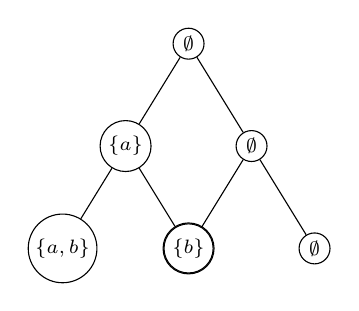
\begin{tikzpicture}[level distance=1.3cm, sibling distance=1.6cm,
  every node/.style={circle,draw,fill=white,inner sep=1.5pt,font=\scriptsize}]
\node {$\emptyset$}
  child { node {$\{a\}$}
    child { node {$\{a,b\}$} }
    child { node {$\{a\}$} }
  }
  child { node {$\emptyset$}
    child { node {$\{b\}$} }
    child { node {$\emptyset$} }
  };
\end{tikzpicture}
\end{center}
\begin{center}
\small Building all subsets of $\{a,b\}$ by deciding ``include $a$?'' then ``include $b$?'' -- each level doubles the count
\end{center}

\bigskip
\begin{definition}[Depth of a set of intervals, Rosen]
For lectures given as time intervals, the \emph{depth} is the maximum number that mutually overlap at any single instant.
\end{definition}

\begin{theorem}[Greedy lecture-scheduling algorithm is optimal, Rosen]
Sorting lectures by start time and greedily assigning each to the first available room needs exactly $\mathrm{depth}$ rooms -- optimal, since no schedule can use fewer than $\mathrm{depth}$ rooms.
\end{theorem}

\begin{algorithm}[H]
\SetAlgoLined
\KwIn{Lectures as intervals $[s_1,f_1],\dots,[s_n,f_n]$}
\KwOut{Room assignment using $\mathrm{depth}$ rooms}
sort lectures by increasing start time $s_i$\;
rooms $\gets$ empty list\;
\ForEach{lecture $L$ in sorted order}{
    \eIf{some room in rooms is free at $L$'s start time}{
        assign $L$ to any such free room\;
    }{
        open a new room, assign $L$ to it\;
    }
}
\caption{Greedy lecture scheduling}
\end{algorithm}
\begin{proof}[Proof sketch, induction on the number of lectures scheduled]
\textbf{Base case}: the first lecture needs $1$ room; $1\le\mathrm{depth}$.

\textbf{Inductive step}: suppose the first $k$ lectures (in start-time order) have been assigned using at most $\mathrm{depth}$ rooms. When lecture $k+1$ arrives, if all currently-open rooms are busy at that moment, the number of busy rooms equals the number of lectures overlapping at that instant -- at most $\mathrm{depth}$. If exactly $\mathrm{depth}$ rooms are busy, opening one more room suffices and keeps the total at $\mathrm{depth}$; if fewer are busy, an existing free room is reused.

By induction, the greedy algorithm never needs more than $\mathrm{depth}$ rooms -- matching the lower bound, hence optimal.
\end{proof}

\begin{center}
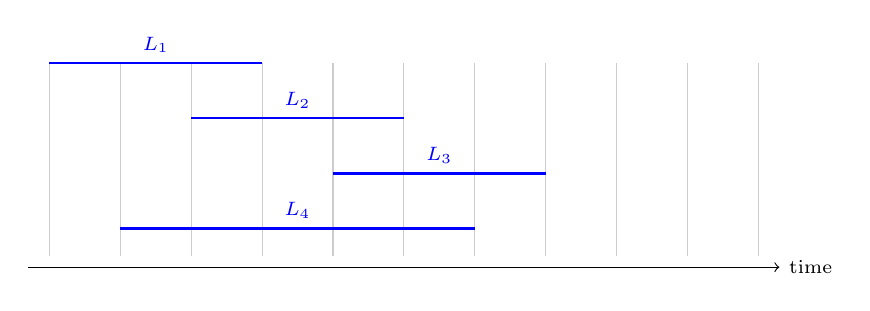
\begin{tikzpicture}[x=0.9cm,y=0.7cm]
\foreach \x in {0,...,10} \draw[gray!40] (\x,0) -- (\x,-3.5);
\draw[thick,blue] (0,0) -- (3,0) node[midway,above] {\scriptsize $L_1$};
\draw[thick,blue] (2,-1) -- (5,-1) node[midway,above] {\scriptsize $L_2$};
\draw[thick,blue] (4,-2) -- (7,-2) node[midway,above] {\scriptsize $L_3$};
\draw[thick,blue] (1,-3) -- (6,-3) node[midway,above] {\scriptsize $L_4$};
\draw[->] (-0.3,-3.7) -- (10.3,-3.7) node[right] {\scriptsize time};
\end{tikzpicture}
\end{center}
\begin{center}
\small $L_1$ and $L_4$ overlap $L_2$; $L_4$ overlaps $L_3$ too -- depth $=2$ at every instant, so $2$ rooms suffice
\end{center}

\bigskip
\begin{theorem}[Odd pie fight -- creative induction]
An odd number $n$ of people stand at pairwise distinct distances. Each simultaneously throws a pie at their \emph{nearest} neighbor. Then at least one person is not hit.
\end{theorem}
\begin{proof}
Induction on odd $n$ (i.e.\ $n=2m+1$, induct on $m\ge1$).

\textbf{Base case} ($n=3$): let $A,B,C$ be the three people. Some pair -- say $A,B$ -- is the \emph{closest} pair overall. Then $A,B$ pie each other; $C$'s pie goes to whichever of $A,B$ is closer to $C$. Either way, $A$ or $B$ is hit twice and $C$ isn't hit -- a survivor exists.

\textbf{Inductive step}: assume the claim for $n=2k+1$ people, and consider $n=2k+3$. Find the overall closest pair $A,B$ -- they pie each other. Remove $A,B$: the other $2k+1$ people still throw pies among themselves at mutually distinct distances -- a valid instance of the same problem. By the inductive hypothesis, this group has a survivor, who also survives in the full group.

By induction, every odd $n$ has a survivor.
\end{proof}

\begin{center}
\begin{tikzpicture}[>={Stealth[length=2mm]}]
\coordinate (A) at (0,0);
\coordinate (B) at (1.5,0.3);
\coordinate (C) at (3.5,1.5);
\fill (A) circle (2pt) node[below] {$A$};
\fill (B) circle (2pt) node[below] {$B$};
\fill (C) circle (2pt) node[above] {$C$};
\draw[->,thick] (A) -- (B);
\draw[->,thick] (B) -- (A);
\draw[->,thick] (C) -- (B);
\end{tikzpicture}
\end{center}
\begin{center}
\small Base case $n=3$: $A,B$ are the closest pair and pie each other; $C$ pies $B$ -- $A$ survives
\end{center}

\begin{note}
False for even $n$: e.g.\ $4$ people can be arranged in two mutual-nearest-neighbor pairs, hitting everyone.
\end{note}

\bigskip
\begin{theorem}[Deficient chessboard tiling, ordinary induction -- Rosen \S\ref{sec:5-1}]
For every $n\ge1$, a $2^n\times2^n$ chessboard with any \emph{one} square removed can be exactly tiled by L-trominoes.
\end{theorem}
\begin{proof}
\textbf{Base case} ($n=1$): a $2\times2$ board minus one square is exactly one L-tromino.

\textbf{Inductive step}: assume every deficient $2^k\times2^k$ board can be tiled. Consider a deficient $2^{k+1}\times2^{k+1}$ board, split into four $2^k\times2^k$ quadrants.

The missing square lies in exactly one quadrant -- deficient, tileable by the inductive hypothesis. Place one L-tromino at the very center, covering the corner cell of \emph{each} of the other three quadrants nearest the center -- making each of those quadrants deficient too.

One central tromino plus four tiled quadrants tiles the whole board.

By induction (using only $P(k)\Rightarrow P(k+1)$ -- this is \emph{ordinary}, not strong, induction, despite the recursive flavor), the claim holds for all $n\ge1$.
\end{proof}

\begin{center}
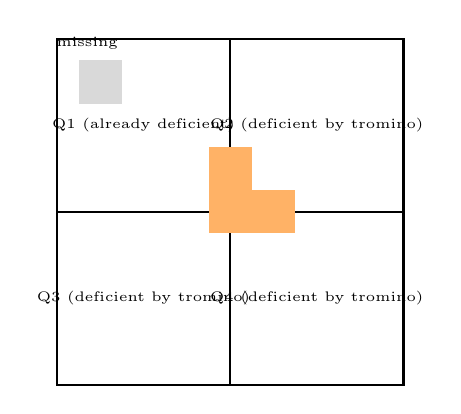
\begin{tikzpicture}[scale=0.55]
\draw[thick] (0,0) rectangle (8,8);
\draw[thick] (4,0) -- (4,8);
\draw[thick] (0,4) -- (8,4);
\fill[gray!30] (0.5,6.5) rectangle (1.5,7.5);
\node at (0.7,7.9) [font=\tiny] {missing};
\fill[orange!60] (3.5,3.5) rectangle (4.5,4.5);
\fill[orange!60] (3.5,4.5) rectangle (4.5,5.5);
\fill[orange!60] (4.5,3.5) rectangle (5.5,4.5);
\node at (2,2) [font=\tiny] {Q3 (deficient by tromino)};
\node at (6,2) [font=\tiny] {Q4 (deficient by tromino)};
\node at (6,6) [font=\tiny] {Q2 (deficient by tromino)};
\node at (2,6) [font=\tiny] {Q1 (already deficient)};
\end{tikzpicture}
\end{center}
\begin{center}
\small One tromino at the center makes the other three quadrants deficient too
\end{center}

\bigskip
\begin{theorem}[Postage stamp problem, Rosen -- strong induction]
Every integer $n \ge 12$ can be formed using only $4$-cent and $5$-cent stamps.
\end{theorem}
\begin{proof}
\textbf{Base cases} ($n=12,13,14,15$):
\[
12=4+4+4, \qquad 13=4+4+5, \qquad 14=4+5+5, \qquad 15=5+5+5.
\]

\textbf{Inductive step}: let $k \ge 15$, and suppose every integer from $12$ to $k$ can be formed. Consider $k+1$. Since $k+1 \ge 16$, we have $k+1-4 \ge 12$, so by the strong inductive hypothesis, $k+1-4$ can be formed. Add one more $4$-cent stamp to form $k+1$.

By strong induction, every $n \ge 12$ can be formed.
\end{proof}

\begin{note}[Why strong induction, not weak]
The step for $k+1$ reaches back to $k+1-4$, which for small $k$ is \emph{not} simply $k$ or $k-1$ -- ordinary induction, which only hands you $S(k)$, isn't enough here.
\end{note}

\bigskip
\begin{theorem}[Existence of prime factorization -- classic strong induction example]
Every integer $n\ge2$ can be written as a product of one or more primes.
\end{theorem}
\begin{proof}
\textbf{Base case} ($n=2$): $2$ itself is prime.

\textbf{Inductive step}: let $k\ge2$, and suppose every integer from $2$ to $k$ has a prime factorization. Consider $n=k+1$.

\textbf{Case 1}: $n$ is prime. Then $n$ itself is its factorization.

\textbf{Case 2}: $n$ is composite, so $n=ab$ for integers $2\le a,b\le n-1=k$. By the strong inductive hypothesis, both $a$ and $b$ have prime factorizations; concatenating them gives a prime factorization of $n=ab$.

Either way, $n$ has a prime factorization.

By strong induction, every $n\ge2$ has one.
\end{proof}

\begin{note}
This needs \emph{strong} induction: the factors $a,b$ of composite $n$ can be much smaller than $n-1$, so the hypothesis must cover \emph{all} smaller values.
\end{note}

\bigskip
\begin{theorem}[Division algorithm -- existence part, via well-ordering]
For $a\in\Z,\ d\in\Z^+$, there exist $q,r\in\Z$ with $a=dq+r$ and $0\le r<d$.
\end{theorem}
\begin{proof}
Consider $S = \{a-dq : q\in\Z,\ a-dq\ge0\}$. $S\subseteq\N$ and $S\neq\emptyset$. By well-ordering, $S$ has a least element $r=a-dq_0$.

We claim $r<d$. If not, $r-d = a-d(q_0+1) \in S$, but $r-d<r$, contradicting minimality of $r$.

So $r<d$, and $q=q_0$ gives $a=dq+r$ with $0\le r<d$.
\end{proof}

\bigskip
\begin{example}[Game-strategy example, Rosen -- strong induction, non-numeric]
Two players alternately remove $1$ or $2$ stones from a pile; the player taking the last stone wins. Claim: the first player wins whenever $n\not\equiv0\pmod3$, and loses whenever $n\equiv0\pmod3$.
\end{example}
\begin{proof}[Proof sketch, strong induction on $n$]
\textbf{Base cases}: $n=1,2$: first player wins. $n=3$: whatever the first player takes, the opponent wins -- first player loses.

\textbf{Inductive step}: assume the claim for all pile sizes less than $n$. If $n\equiv0\pmod3$: any move leaves $n-1$ or $n-2$, neither $\equiv0\pmod3$, so the opponent wins -- first player loses. If $n\not\equiv0\pmod3$: the first player can always leave a multiple of $3$, putting the opponent in a losing position.
\end{proof}

\bigskip
\begin{definition}[Simple polygon, diagonal]
A \emph{simple polygon} is a polygon whose sides do not cross. A \emph{diagonal} is a line segment connecting two non-adjacent vertices that lies entirely inside the polygon.
\end{definition}

\begin{lemma}[Every simple polygon with $\ge4$ sides has a diagonal]
\end{lemma}
\begin{proof}[Proof sketch]
Take the leftmost vertex $v$ and its two neighbors $u,w$. If segment $uw$ lies inside the polygon, it is a diagonal. Otherwise, some vertex lies inside triangle $uvw$; take the one farthest from line $uw$ -- the segment from $v$ to that vertex is a diagonal.
\end{proof}

\bigskip
\begin{theorem}[Triangulation of simple polygons -- Rosen, strong induction]
Every simple polygon with $n\ge3$ sides can be triangulated into exactly $n-2$ triangles using $n-3$ non-crossing diagonals.
\end{theorem}
\begin{proof}
\textbf{Base case} ($n=3$): a triangle is already $1=3-2$ triangle, using $0=3-3$ diagonals.

\textbf{Inductive step}: let $k\ge3$, and suppose every simple polygon with fewer than $k+1$ sides can be triangulated as claimed. Let $P$ have $n=k+1\ge4$ sides.

By the lemma, $P$ has a diagonal $d$, splitting $P$ into $P_1,P_2$ sharing edge $d$, with $n_1+n_2 = n+2$.

Since $3\le n_1,n_2\le n-1$, the strong inductive hypothesis applies to both: $P_1$ triangulates into $n_1-2$ triangles, $P_2$ into $n_2-2$.

Together: $(n_1-2)+(n_2-2) = n-2$ triangles, using $1+(n_1-3)+(n_2-3) = n-3$ diagonals.

By strong induction, the claim holds for all $n\ge3$.
\end{proof}

\begin{center}
\begin{tikzpicture}[scale=1.1]
\coordinate (v1) at (90:2);
\coordinate (v2) at (150:2);
\coordinate (v3) at (210:2);
\coordinate (v4) at (270:2);
\coordinate (v5) at (330:2);
\coordinate (v6) at (30:2);
\draw[thick] (v1)--(v2)--(v3)--(v4)--(v5)--(v6)--cycle;
\draw[dashed] (v1)--(v3);
\draw[dashed] (v1)--(v4);
\draw[dashed] (v1)--(v5);
\foreach \p in {v1,v2,v3,v4,v5,v6} {\fill (\p) circle (1.5pt);}
\node at ($(v1)+(0,0.35)$) {$v_1$};
\node at ($(v2)+(-0.35,0.15)$) {$v_2$};
\node at ($(v3)+(-0.35,-0.15)$) {$v_3$};
\node at ($(v4)+(0,-0.35)$) {$v_4$};
\node at ($(v5)+(0.35,-0.15)$) {$v_5$};
\node at ($(v6)+(0.35,0.15)$) {$v_6$};
\end{tikzpicture}
\end{center}
\begin{center}
\small A hexagon triangulated by $3$ diagonals into $4$ triangles
\end{center}

\bigskip
\begin{theorem}[The matchstick game -- Rosen \S\ref{sec:5-2}, Example 4, strong induction]
Two piles start with $n$ matches each. Players alternate turns; each turn, remove any positive number of matches from \emph{one} pile. The player who removes the last match wins. Then the \emph{second} player can always force a win, for every $n\ge1$.
\end{theorem}
\begin{proof}
Let $P(n)$: ``if both piles start with $n$ matches, the second player can force a win.''

\textbf{Base case} ($n=1$): the first player must remove the single match from one pile; the second takes the other and wins.

\textbf{Inductive step}: let $k\ge1$, suppose $P(1),\dots,P(k)$ hold. Whatever the first player does -- removing $r$ matches from one pile -- the second mirrors on the other pile.

\begin{itemize}
    \item If $r=k+1$: the second empties the other pile, winning immediately.
    \item If $r<k+1$: both piles now have equal size $k+1-r\le k$ -- by $P(k+1-r)$, the second player can force a win from there.
\end{itemize}

Either way, the second player wins. By strong induction, $P(n)$ holds for all $n\ge1$.
\end{proof}

\bigskip
\begin{theorem}[Round-robin tournament ranking -- classic strong induction example]
In a round-robin tournament with $n$ players, the players can be labeled $p_1,\dots,p_n$ such that $p_i$ beats $p_{i+1}$ for every $i$.
\end{theorem}
\begin{proof}
\textbf{Base case} ($n=1$): trivial.

\textbf{Inductive step}: let $k\ge1$, suppose the claim holds for at most $k$ players. Consider $k+1$ players. Pick any player $x$; let $B$ = players who beat $x$, $L$ = players $x$ beats, so $|B|,|L|\le k$.

By the inductive hypothesis, $B$ has a chain ordering $b_1,\dots,b_{|B|}$, and $L$ has $\ell_1,\dots,\ell_{|L|}$. Concatenate:
\[
b_1,\dots,b_{|B|},\ x,\ \ell_1,\dots,\ell_{|L|}.
\]
The joins $b_{|B|}\to x$ and $x\to\ell_1$ hold by definition of $B,L$.

By strong induction, the claim holds for all $n\ge1$.
\end{proof}
\subsection{Induction: extended example}
\label{sec:3-12}
% CN 3.12 (omega, advanced) -- CN's own extended example: injections into a shortlist relation

\begin{note}[Setup]
$m$ job positions $A$ ($|A|=m$), $n$ applicants $B$ ($|B|=n$), a \emph{shortlist relation} $S \subseteq A\times B$.

For $X \subseteq A$, write
\[
S(X) = \bigcup_{a\in X} S(a)
\]
(\S\ref{sec:2-13} notation) for the combined shortlist of positions in $X$.

A valid assignment (every position filled, no applicant doubled) is exactly an \emph{injection} $A \to B$ contained in $S$.
\end{note}

\bigskip
\begin{theorem}[Necessity, CN Thm 20]
If $S$ contains an injection with domain $A$, then $|X| \le |S(X)|$ for every $X \subseteq A$.
\end{theorem}
\begin{proof}
An injection assigns distinct applicants to distinct positions, so the positions in $X$ alone already require $|X|$ distinct applicants, all drawn from $S(X)$.
\end{proof}

\bigskip
\begin{theorem}[Sufficiency, CN Thm 21 -- the converse, by induction on $|A|$]
If $|X| \le |S(X)|$ for every $X \subseteq A$, then $S$ contains an injection with domain $A$.
\end{theorem}
\begin{proof}
Induction on $m=|A|$.

\medskip
\textbf{Base case} ($m=1$):

$A=\{a\}$; the condition with $X=\{a\}$ gives $|S(a)|\ge1$, so pick any $(a,b)\in S$ -- this single pair is an injection with domain $A$.

\medskip
\textbf{Inductive step}: assume the theorem for all relations with domain-size $\le m$. Let $|A|=m+1$ and suppose $|X|\le|S(X)|$ for all $X\subseteq A$.

\medskip
\textbf{Case 1}: every nonempty proper $X\subsetneq A$ has \emph{strict} slack,
\[
|X| \le |S(X)|-1.
\]

Pick any $(a,b)\in S$. Restrict $S$ to
\[
T = S \cap \big((A\setminus\{a\})\times(B\setminus\{b\})\big),
\]
i.e.\ drop $a$ and $b$. For $X\subseteq A\setminus\{a\}$, the strict slack gives $|T(X)|\ge|X|$ even after excluding $b$.

Since $|A\setminus\{a\}|=m$, the inductive hypothesis applies: $T$ contains an injection $g$ with domain $A\setminus\{a\}$.

Then $g \cup \{(a,b)\}$ is an injection with domain $A$, contained in $S$.

\medskip
\textbf{Case 2}: some nonempty proper $X\subsetneq A$ has \emph{exact} fit,
\[
|X|=|S(X)|.
\]

Apply the inductive hypothesis to $S$ restricted to $X\times S(X)$ (domain size $|X|\le m$): get an injection $g: X \to S(X)$.

For the rest, $A\setminus X$: for any $Z\subseteq A\setminus X$, a counting argument using $|X\cup Z|\le|S(X\cup Z)|$ and $|S(X)|=|X|$ shows
\[
|Z| \le |S(Z)\setminus S(X)|.
\]

So the relation $U = S \cap \big((A\setminus X)\times(B\setminus S(X))\big)$ satisfies the same slack condition on domain $A\setminus X$ (size $\le m$), so by the inductive hypothesis, $U$ contains an injection $h$ with domain $A\setminus X$.

Since $g,h$ have disjoint domains ($X$, $A\setminus X$) and disjoint codomains ($S(X)$, $B\setminus S(X)$), $g\cup h$ is an injection with domain $A$, contained in $S$.

\medskip
Cases 1 and 2 are exhaustive, completing the inductive step. By induction, the theorem holds for all $m$.
\end{proof}

\bigskip
\begin{corollary}[CN Cor. 22]
$S \subseteq A\times B$ contains an injection with domain $A$ $\iff$ $|X|\le|S(X)|$ for every $X\subseteq A$.
\end{corollary}

\begin{note}[Why this matters]
This gives easily \emph{verifiable} evidence in both directions: a ``yes'' is witnessed by the injection itself (checkable directly); a ``no'' is witnessed by a single offending set $X$ with $|X|>|S(X)|$ -- no need to search the whole space of possible assignments. This is a defect-form statement of \emph{Hall's marriage theorem}.
\end{note}

\subsection{Mathematical induction and statistical induction}
\label{sec:3-13}
% CN 3.13

\begin{note}
\emph{Statistical induction} (drawing general conclusions from data, typically under randomness, tolerating some error) is unrelated to \emph{mathematical induction} despite the shared name. Statistical induction is not logical deduction and cannot serve as a proof step; mathematical induction is a rigorous deductive technique. Don't conflate the two.
\end{note}

\subsection{Programs and proofs}
\label{sec:3-14}
% CN 3.14 / Rosen 5.4-5.5

\begin{note}[The analogy, point by point]
\begin{itemize}
    \item \textbf{Statements}: a program is a sequence of statements in a programming language; a proof is a sequence of statements in mathematical language (augmented by precise natural language).
    \item \textbf{Variables}: both use named references to objects; program variables have allocated memory, proof variables do not.
    \item \textbf{Sequential dependence}: a program statement uses only the most recently computed value of a variable, never a later one; a proof statement is justified only by \emph{earlier} statements, never later ones.
    \item \textbf{Branching}: an if-statement picks a branch by a logical condition; proof by cases (\S\ref{sec:3-8}) covers all situations via a finite set of logical conditions.
    \item \textbf{Calling other code}: a program calls other functions/programs; a proof invokes previously proved theorems.
    \item \textbf{Repetition}: a program repeats via loops or recursion; a proof repeats (in effect) via mathematical induction.
    \item \textbf{Bugs}: a program with a bug may crash on some inputs but still work on others; a proof with a genuine gap is \emph{not a proof at all} -- it must be repaired, or the claim may simply be false.
\end{itemize}
\end{note}

\begin{note}[Loops $\leftrightarrow$ induction, Rosen \S\ref{sec:5-5}]
Proving a loop computes the correct result typically uses a \emph{loop invariant}: a statement $I$ that (i) holds before the loop begins, and (ii) if true before an iteration, remains true after it -- exactly the base case and inductive step of mathematical induction, applied to ``iteration number.'' If $I$ also implies the desired postcondition once the loop terminates, this establishes \emph{partial correctness}.
\end{note}

\begin{note}[Recursion $\leftrightarrow$ structural induction, Rosen \S\ref{sec:5-3}-5.4]
Proving a recursive function correct mirrors proving a recursively-defined structure has some property: verify the function is correct on the base case(s) of the recursion, then verify that, \emph{assuming} correctness on smaller/simpler inputs (the recursive calls), the function is correct on the current input -- the direct analogue of an inductive hypothesis.
\end{note}

\begin{note}[Programming paradigms]
Just as learning multiple programming paradigms (procedural, object-oriented, logic, functional) improves programming skill generally, learning to write rigorous proofs -- a distinct ``paradigm'' of precise reasoning -- transfers back to writing better, more carefully-reasoned programs.
\end{note}

% ============================================================
% CHAPTER 4 --- PROPOSITIONAL LOGIC  (CN Ch.4, §4.1-4.21)
% ============================================================
\newpage
\section{Propositional Logic}

\subsection{Truth values}
\label{sec:4-1}
% CN 4.1 / Rosen 1.1

\begin{definition}[Truth values]
Logic (classical, two-valued) is built on two \emph{truth values}: \emph{True} ($T$) and \emph{False} ($F$).
\end{definition}

\begin{note}
Physically, truth values may correspond to presence/absence of electrical current, magnetisation, a switch's on/off state, etc. -- the abstraction lets us reason about logic independently of implementation. The \emph{bit} (0 or 1) is a closely related abstraction: $F \leftrightarrow 0$, $T \leftrightarrow 1$.
\end{note}

\subsection{Boolean variables}
\label{sec:4-2}
% CN 4.2

\begin{definition}[Boolean / propositional variable]
A \emph{Boolean variable} (or \emph{propositional variable}) is a variable whose value is $T$ or $F$.
\end{definition}

\subsection{Propositions}
\label{sec:4-3}
% CN 4.3 / Rosen 1.1

\begin{definition}[Proposition, Rosen]
A \emph{proposition} is a declarative sentence that is either true or false, but not both.
\end{definition}

\begin{example}[Propositions]
$1+1=2$ (true); ``The earth is flat.'' (false); ``It will rain tomorrow.'' (a proposition -- has a definite truth value, even if unknown to us right now).
\end{example}

\begin{example}[Not propositions]
Questions (``Come and work for us!''), nonsensical or non-declarative sentences (Lewis Carroll's ``'Twas brillig...''), and self-referential sentences with no consistent truth value (``This statement is false.'') are not propositions.
\end{example}

\begin{note}[Naming a proposition]
A proposition may be named by a Boolean variable, e.g.\ let $X$ be the proposition $1+1=2$; then $X$'s truth value is $T$.
\end{note}

\subsection{Logical operations}
\label{sec:4-4}
% CN 4.4 / Rosen 1.1

\begin{note}[The basic connectives]
\begin{center}
\begin{tabular}{ll}
Not & $\neg$ \\
And & $\wedge$ \\
Or & $\vee$ \\
Implies & $\implies$ \\
Equivalence & $\iff$
\end{tabular}
\end{center}
Logical operations combining propositions are also called \emph{connectives}; in hardware they are implemented as \emph{logic gates}.
\end{note}

\subsection{Negation}
\label{sec:4-5}
% CN 4.5 / Rosen 1.1

\begin{definition}[Negation]
For proposition $P$, $\neg P$ is true iff $P$ is false.
\[
\begin{array}{c|c}
P & \neg P \\ \hline
F & T \\
T & F
\end{array}
\]
\end{definition}

\begin{theorem}[Double negation]
\[
\neg\neg P = P.
\]
\end{theorem}

\begin{note}[Analogy with set complement]
Negation mirrors complementation (\S\ref{sec:1-11}): both give the ``completely opposite'' outcome, and applying either twice returns the original. If $P$ is the proposition $x \in A$, then $\neg P$ is $x \in \overline{A}$: e.g.\ $\neg(\sqrt2 \in \Q)$ is the same as $\sqrt2 \in \overline{\Q}$ (equivalently $\sqrt2 \notin \Q$).
\end{note}

\subsection{Conjunction}
\label{sec:4-6}
% CN 4.6 / Rosen 1.1

\begin{definition}[Conjunction]
For propositions $P,Q$: $P \wedge Q$ (``$P$ and $Q$'') is true iff \emph{both} $P$ and $Q$ are true.
\[
\begin{array}{cc|c}
P & Q & P \wedge Q \\ \hline
F & F & F \\
F & T & F \\
T & F & F \\
T & T & T
\end{array}
\]
\end{definition}

\begin{note}[Analogy with set intersection]
For object $x$ and sets $A,B$:
\[
(x \in A) \wedge (x \in B) \iff x \in A \cap B, \qquad A \cap B = \{x : x\in A \wedge x \in B\}
\]
(restating \S\ref{sec:1-12}'s definition using $\wedge$).
\end{note}

\begin{definition}[Generalized (n-ary) conjunction, Rosen]
For propositions $P_1,\dots,P_n$:
\[
P_1 \wedge P_2 \wedge \cdots \wedge P_n
\]
is true iff \emph{every} $P_i$ is true.
\end{definition}

\begin{example}[Translating English ``and'', Rosen]
``You can access the internet from campus only if you are a computer science major or you are not a freshman'' involves nested connectives; more simply, ``It is below freezing and snowing'' translates directly as $P \wedge Q$ for $P=$``it is below freezing'', $Q=$``it is snowing''. Care is needed when English sentences bury an implicit ``and'' inside a single clause (e.g.\ ``$x$ is between $2$ and $5$'' is really $(x>2)\wedge(x<5)$).
\end{example}

\subsection{Disjunction}
\label{sec:4-7}
% CN 4.7 / Rosen 1.1

\begin{definition}[Disjunction]
For propositions $P,Q$: $P \vee Q$ (``$P$ or $Q$'') is true iff \emph{at least one} of $P,Q$ is true.
\[
\begin{array}{cc|c}
P & Q & P \vee Q \\ \hline
F & F & F \\
F & T & T \\
T & F & T \\
T & T & T
\end{array}
\]
\end{definition}

\begin{note}[Inclusive, not exclusive]
This is the \emph{inclusive-or}: true even when \emph{both} $P,Q$ are true. Contrast with \emph{exclusive-or} (\S\ref{sec:4-11}), true precisely when \emph{exactly one} holds.
\end{note}

\begin{example}[English ``or'' is ambiguous, Rosen]
``Students who have taken CS100 or CS200 may take this class'' -- inclusive: having taken both still qualifies. ``Soup or salad comes with this entree'' -- exclusive in ordinary restaurant use: you get one, not both, even though the sentence uses the same word ``or.'' Mathematical $\vee$ always means \emph{inclusive}-or unless stated otherwise; natural language is not reliable here.
\end{example}

\begin{note}[Analogy with set union]
For object $x$ and sets $A,B$:
\[
(x \in A) \vee (x \in B) \iff x \in A \cup B, \qquad A \cup B = \{x : x\in A \vee x \in B\}
\]
(restating \S\ref{sec:1-12}'s definition using $\vee$).
\end{note}

\begin{note}[Operator precedence so far, Rosen]
Among the connectives introduced up to this point, precedence (highest to lowest) is:
\[
\neg \ > \ \wedge \ > \ \vee.
\]
So $\neg P \vee Q$ means $(\neg P) \vee Q$, and $P \wedge Q \vee R$ means $(P \wedge Q) \vee R$ -- parenthesize explicitly whenever there's any doubt.
\end{note}

\subsection{De Morgan's Laws}
\label{sec:4-8}
% CN 4.8 / Rosen 1.3

\begin{theorem}[De Morgan's Laws for propositions]
\[
\neg(P \vee Q) = \neg P \wedge \neg Q, \qquad \neg(P \wedge Q) = \neg P \vee \neg Q.
\]
\end{theorem}

\bigskip
\begin{proof}[Proof of the first law, by truth table]
\[
\begin{array}{cc|c|c|cc|c}
P & Q & P\vee Q & \neg(P\vee Q) & \neg P & \neg Q & \neg P \wedge \neg Q \\ \hline
F & F & F & T & T & T & T \\
F & T & T & F & T & F & F \\
T & F & T & F & F & T & F \\
T & T & T & F & F & F & F
\end{array}
\]
The columns for $\neg(P\vee Q)$ and $\neg P \wedge \neg Q$ agree in every row, so the two expressions are \emph{logically equivalent} -- true or false together, for every assignment of truth values to $P,Q$.
\end{proof}

\bigskip
\begin{note}[Building the table incrementally]
The table is constructed left to right, each column using only earlier columns: start with all combinations of $P,Q$; build $P\vee Q$; negate it to get $\neg(P\vee Q)$; separately build $\neg P$ and $\neg Q$; conjoin them to get $\neg P \wedge \neg Q$. Comparing the two target columns (highlighted) completes the proof.
\end{note}

\bigskip
\begin{note}[Deriving the second law from the first]
Rather than repeating the truth-table argument, the second law follows from the first by substitution: replace $P,Q$ with $\neg P, \neg Q$ in the first law and simplify using double negation (\S\ref{sec:4-5}).
\end{note}

\bigskip
\begin{theorem}[Generalized De Morgan's law, CN Thm 23]
For all $n$:
\[
\neg(P_1 \vee \cdots \vee P_n) = \neg P_1 \wedge \cdots \wedge \neg P_n.
\]
\end{theorem}
\begin{proof}
\begin{align*}
\text{LHS is true} &\iff P_1 \vee \cdots \vee P_n \text{ is false} \\
&\iff P_1,\dots,P_n \text{ are all false} \\
&\iff \neg P_1,\dots,\neg P_n \text{ are all true} \\
&\iff \text{RHS is true.}
\end{align*}
\end{proof}

\begin{note}
This argument works for \emph{every} $n$ at once -- unlike the truth-table method, which would need a separate (and infinite) family of tables, one per $n$.
\end{note}

\bigskip
\begin{note}[Correspondence with the set-theoretic De Morgan's laws]
Compare directly with \S\ref{sec:1-11}'s Theorem (De Morgan's laws for sets): $\overline{A\cup B} = \overline A \cap \overline B$ and $\overline{A\cap B} = \overline A \cup \overline B$ are exactly the propositional laws above, applied to the propositions $x\in A$ and $x\in B$.
\end{note}

\bigskip
\begin{note}[Rosen: naming logical equivalence]
Two compound propositions are \emph{logically equivalent} iff their truth tables are identical in every row -- written $P \equiv Q$ or $P \iff Q$ (a \emph{tautology}, true under every assignment; formalized further in \S\ref{sec:4-12}).
\end{note}

\subsection{Implication}
\label{sec:4-9}
% CN 4.9 / Rosen 1.1

\begin{definition}[Implication]
$P \implies Q$ (``if $P$ then $Q$'') is false only when $P$ is true and $Q$ is false.
\[
\begin{array}{cc|c}
P & Q & P \implies Q \\ \hline
F & F & T \\
F & T & T \\
T & F & F \\
T & T & T
\end{array}
\]
\end{definition}

\begin{note}[Rosen's phrasings]
$P \implies Q$ reads: ``if $P$ then $Q$''; ``$P$ only if $Q$''; ``$P$ is sufficient for $Q$''; ``$Q$ is necessary for $P$''; ``$Q$ whenever $P$''.
\end{note}

\subsection{Equivalence}
\label{sec:4-10}
% CN 4.10 / Rosen 1.1

\begin{definition}[Equivalence / biconditional]
$P \iff Q$ is true iff $P,Q$ have the same truth value.
\[
\begin{array}{cc|c}
P & Q & P \iff Q \\ \hline
F & F & T \\
F & T & F \\
T & F & F \\
T & T & T
\end{array}
\]
\end{definition}

\begin{theorem}
\[
P \iff Q \quad \equiv \quad (P \implies Q) \wedge (Q \implies P).
\]
\end{theorem}

\begin{note}[Rosen's phrasing]
$P \iff Q$ reads: ``$P$ if and only if $Q$''; ``$P$ is necessary and sufficient for $Q$''.
\end{note}

\begin{note}[Analogy with set equality]
$x\in A \iff x\in B$ for all $x$ is exactly $A=B$ (\S\ref{sec:1-6}).
\end{note}

\subsection{Exclusive-or}
\label{sec:4-11}
% CN 4.11 / Rosen 1.1

\begin{definition}[Exclusive-or]
$P \oplus Q$ is true iff exactly one of $P,Q$ is true.
\[
\begin{array}{cc|c}
P & Q & P \oplus Q \\ \hline
F & F & F \\
F & T & T \\
T & F & T \\
T & T & F
\end{array}
\]
\end{definition}

\begin{theorem}
\[
P \oplus Q = \neg(P \iff Q).
\]
\end{theorem}

\bigskip
\begin{theorem}[Generalized XOR parity, CN Thm 24]
For all $n$ and propositions $P_1,\dots,P_n$: $P_1\oplus\cdots\oplus P_n$ is true iff an \emph{odd} number of the $P_i$ are true.
\end{theorem}
\begin{proof}
Induction on $n$.

\medskip
\textbf{Base case} ($n=1$): $P_1$ alone is true iff exactly $1$ (odd) of it is true.

\medskip
\textbf{Inductive step}: assume the claim for $k$ propositions. Then
\[
P_1\oplus\cdots\oplus P_{k+1} = (P_1\oplus\cdots\oplus P_k) \oplus P_{k+1}.
\]
By the inductive hypothesis, the first factor is $T$ iff an odd number of $P_1,\dots,P_k$ are true, else $F$. Checking all four combinations of (that factor, $P_{k+1}$) against $\oplus$'s truth table shows the result is $T$ exactly when the \emph{total} count of true propositions among $P_1,\dots,P_{k+1}$ is odd.

\medskip
By induction, the claim holds for all $n$.
\end{proof}

\begin{note}[Analogy with symmetric difference]
$x \in A_1 \triangle \cdots \triangle A_n \iff (x\in A_1)\oplus\cdots\oplus(x\in A_n)$ (\S\ref{sec:1-13}).
\end{note}

\bigskip
\begin{example}[Knights and knaves, Rosen -- a harder puzzle]
On an island, every inhabitant is either a \emph{knight} (always tells the truth) or a \emph{knave} (always lies). $A$ says: ``$B$ is a knave.'' $B$ says: ``$A$ and $I$ are of opposite types.''

Let $a$ = ``$A$ is a knight'', $b$ = ``$B$ is a knight.'' $A$'s statement, if $A$ is a knight, must be true, and if $A$ is a knave, must be false -- i.e.\ $a \iff \neg b$. $B$'s statement ``$A,B$ are opposite types'' is $a \oplus b$; by the same reasoning, $b \iff (a\oplus b)$.

From $a \iff \neg b$: exactly one of $a,b$ is true. Substitute into $b \iff (a\oplus b)$: since exactly one of $a,b$ is true, $a\oplus b$ is true, so this forces $b$ true, hence $a$ false. So $A$ is a knave, $B$ is a knight.
\end{example}

\subsection{Tautologies and logical equivalence}
\label{sec:4-12}
% CN 4.12 / Rosen 1.3

\begin{definition}[Tautology]
A proposition that is true under every assignment of truth values (every row of its truth table is $T$).
\end{definition}

\begin{definition}[Logical equivalence]
$P \equiv Q$ (written $P=Q$) iff their truth tables are identical, iff $P\iff Q$ is a tautology.
\end{definition}

\begin{note}[Key equivalences]
\[
\neg\neg P = P, \qquad \neg(P\vee Q)=\neg P\wedge\neg Q, \qquad \neg(P\wedge Q)=\neg P\vee\neg Q,
\]
\[
P\implies Q = \neg P \vee Q, \qquad P\iff Q = (P\implies Q)\wedge(Q\implies P),
\]
\[
P\oplus Q = \neg(P\iff Q) = P \iff \neg Q.
\]
\end{note}

\bigskip
\begin{theorem}[Exportation law, Rosen -- harder derivation]
\[
(P \wedge Q) \implies R \ \equiv \ P \implies (Q \implies R).
\]
\end{theorem}
\begin{proof}
Using $X\implies Y = \neg X \vee Y$ repeatedly:
\begin{align*}
(P\wedge Q)\implies R &= \neg(P\wedge Q)\vee R = (\neg P \vee \neg Q)\vee R && \text{(De Morgan's)}\\
&= \neg P \vee (\neg Q \vee R) && \text{(associativity of $\vee$)}\\
&= \neg P \vee (Q \implies R) \\
&= P \implies (Q \implies R).
\end{align*}
\end{proof}

\subsection{History}
\label{sec:4-13}
% CN 4.13

\subsection{Distributive Laws}
\label{sec:4-14}
% CN 4.14 / Rosen 1.3

\begin{theorem}[Distributive laws]
\[
P \wedge (Q\vee R) = (P\wedge Q)\vee(P\wedge R), \qquad P \vee (Q\wedge R) = (P\vee Q)\wedge(P\vee R).
\]
\end{theorem}

\bigskip
\begin{theorem}[Absorption laws, Rosen -- derived, not axiomatic]
\[
P \vee (P\wedge Q) = P, \qquad P \wedge (P\vee Q) = P.
\]
\end{theorem}
\begin{proof}
\begin{align*}
P \vee (P\wedge Q) &= (P\wedge T)\vee(P\wedge Q) && \text{(identity: $P = P\wedge T$)}\\
&= P \wedge (T \vee Q) && \text{(distributive law)}\\
&= P \wedge T && \text{(domination: $T\vee Q=T$)}\\
&= P.
\end{align*}
The second identity is the dual (swap $\wedge \leftrightarrow \vee$, $T \leftrightarrow F$ throughout).
\end{proof}

\subsection{Laws of Boolean algebra}
\label{sec:4-15}
% CN 4.15 / Rosen 1.3 (Table of Logical Equivalences)

\begin{note}[Full table, dual pairs]
\[
\neg\neg P = P
\]
\[
\neg T = F, \quad \neg F = T
\]
\[
P\wedge Q = Q\wedge P, \qquad P\vee Q = Q\vee P \quad \text{(commutative)}
\]
\[
(P\wedge Q)\wedge R = P\wedge(Q\wedge R), \qquad (P\vee Q)\vee R = P\vee(Q\vee R) \quad \text{(associative)}
\]
\[
P\wedge P = P, \qquad P\vee P = P \quad \text{(idempotent)}
\]
\[
P\wedge\neg P = F, \qquad P\vee\neg P = T \quad \text{(complement)}
\]
\[
P\wedge T = P, \qquad P\vee F = P \quad \text{(identity)}
\]
\[
P\wedge F = F, \qquad P\vee T = T \quad \text{(domination)}
\]
\[
P\wedge(Q\vee R)=(P\wedge Q)\vee(P\wedge R), \qquad P\vee(Q\wedge R)=(P\vee Q)\wedge(P\vee R) \quad \text{(distributive)}
\]
\[
\neg(P\vee Q)=\neg P\wedge\neg Q, \qquad \neg(P\wedge Q)=\neg P\vee\neg Q \quad \text{(De Morgan's)}
\]
\end{note}

\bigskip
\begin{example}[Algebraic proof, Rosen -- harder chain]
Show $\neg(P\implies Q) \equiv P \wedge \neg Q$.
\begin{align*}
\neg(P\implies Q) &= \neg(\neg P \vee Q) \\
&= \neg\neg P \wedge \neg Q && \text{(De Morgan's)}\\
&= P \wedge \neg Q && \text{(double negation)}.
\end{align*}
\end{example}

\subsection{Disjunctive Normal Form}
\label{sec:4-16}
% CN 4.16 / Rosen 1.3 (min-terms)

\begin{definition}[Literal]
A logical variable, unnegated or negated once ($X$ or $\neg X$).
\end{definition}

\begin{definition}[DNF]
A disjunction of conjunctions of literals.
\end{definition}

\begin{note}[Constructing DNF from a truth table]
For each row where the expression is $T$: form the conjunction of literals matching that row ($X$ if $X=T$ in that row, $\neg X$ if $X=F$); disjoin all such conjunctions.
\end{note}

\bigskip
\begin{example}[Majority function of 3 variables, Rosen-style -- harder]
$\mathrm{Maj}(X,Y,Z)$ is true iff at least two of $X,Y,Z$ are true.
\[
\begin{array}{ccc|c}
X&Y&Z&\mathrm{Maj}\\\hline
F&F&F&F\\ F&F&T&F\\ F&T&F&F\\ F&T&T&T\\
T&F&F&F\\ T&F&T&T\\ T&T&F&T\\ T&T&T&T
\end{array}
\]
DNF (four true rows):
\[
\mathrm{Maj}(X,Y,Z) = (\neg X\wedge Y\wedge Z)\vee(X\wedge\neg Y\wedge Z)\vee(X\wedge Y\wedge \neg Z)\vee(X\wedge Y\wedge Z).
\]
\end{example}

\begin{note}[Cost of DNF]
Every expression has an equivalent DNF, but the number of parts can be as large as $2^k$ for $k$ variables -- exponential blow-up. DNF makes \emph{satisfiability} easy to certify (any one part gives a satisfying assignment) but gives no efficient way to certify a \emph{tautology}.
\end{note}

\subsection{Conjunctive Normal Form}
\label{sec:4-17}
% CN 4.17 / Rosen 1.3

\begin{definition}[CNF]
A conjunction of \emph{clauses}, each a disjunction of literals.
\end{definition}

\begin{note}[Duality with DNF, via De Morgan's]
If $P$ is in CNF, $\neg P$ -- negation of a conjunction of disjunctions -- becomes, via repeated De Morgan's and double negation, a disjunction of conjunctions of literals: DNF. So CNF and DNF are dual representations.
\end{note}

\begin{note}[Converting truth table $\to$ CNF]
Negate the output column; build DNF for $\neg P$; negate that expression; apply De Morgan's to push the negation inward into CNF form.
\end{note}

\bigskip
\begin{note}[3-SAT, Rosen/CS -- harder, beyond CN]
When every CNF clause has exactly $3$ literals, satisfiability is the classical \emph{3-SAT} problem -- the canonical NP-complete problem (Cook--Levin theorem). This is why CNF, not DNF, is the standard input format for SAT solvers: checking DNF satisfiability is trivial, but CNF satisfiability is computationally hard in general, which is exactly the structure that makes CNF expressive enough to encode real combinatorial problems.
\end{note}

\subsection{Satisfiability}
% New section (not in CN ToC) -- Rosen 1.3

\begin{definition}[Satisfiable, unsatisfiable]
A compound proposition is \emph{satisfiable} if some assignment of truth values to its variables makes it true (a \emph{satisfying assignment}); otherwise it is \emph{unsatisfiable}.
\end{definition}

\begin{note}[Satisfiability and normal forms]
In DNF (\S\ref{sec:4-16}), satisfiability is trivial to check: any one disjunct with no variable appearing both negated and unnegated gives a satisfying assignment directly. In CNF (\S\ref{sec:4-17}), determining satisfiability in general is the SAT problem -- NP-complete (\S\ref{sec:4-17}'s note on 3-SAT).
\end{note}

\bigskip
\begin{example}[The $n$-queens problem as satisfiability -- CN Ex.\,4.8 / Rosen \S1.3]
\label{ex:nqueens}
Place $n$ queens on an $n\times n$ chessboard so that no two attack each other (same row, column, or diagonal). Variables $x_{i,j}$ $(1\le i,j\le n)$: true iff a queen occupies row $i$, column $j$.

\medskip
\noindent\textbf{Clause $\Leftrightarrow$ at-most-one, symbolically.} For any $x_1,\dots,x_m$,
\[
\bigwedge_{1\le j<k\le m}(\neg x_j\vee\neg x_k) \ \equiv\ \neg\exists j\ne k\ (x_j\wedge x_k) \ \equiv\ \text{``at most one $x_i$ is true''},
\]
since each pairwise clause $\neg x_j\vee\neg x_k \equiv \neg(x_j\wedge x_k)$ rules out that particular pair, and ranging over all $\binom m2$ pairs rules out every pair.

\medskip
\noindent\textbf{Exactly one queen per row $i$}:
\[
\underbrace{x_{i,1}\vee\cdots\vee x_{i,n}}_{\text{at least one}}
\qquad\wedge\qquad
\bigwedge_{1\le j<k\le n}\underbrace{(\neg x_{i,j}\vee\neg x_{i,k})}_{\text{at most one}}.
\]
Clause count per row: $1+\binom n2$. Over $n$ rows:
\[
n\binom n2 = n\cdot\frac{n(n-1)}2 = \frac{n^3-n^2}2 = \Theta(n^3).
\]

\medskip
\noindent\textbf{At most one queen per column $j$}:
\[
\bigwedge_{j=1}^n\ \bigwedge_{1\le i<k\le n}(\neg x_{i,j}\vee\neg x_{k,j}), \qquad n\binom n2=\Theta(n^3)\text{ clauses}.
\]

\smallskip
\noindent\emph{Why no "at least one" clause is needed (pigeonhole, formalised).} Let $S=\{(i,j):x_{i,j}=\mathrm{true}\}$ under any satisfying assignment. The row constraints give a bijection $\sigma:\{1,\dots,n\}\to\{1,\dots,n\}$, $\sigma(i)=j$ where $(i,j)\in S$ (well-defined and total since each row has exactly one true variable). The column constraints say $\sigma$ is injective. A total injective function on a finite set of size $n$ to itself is a bijection, so $\sigma$ is surjective too -- every column is hit exactly once, with no separate clause required.

\medskip
\noindent\textbf{At most one queen per diagonal}: for $(i,j)\ne(k,l)$ with $|i-k|=|j-l|$,
\[
\neg x_{i,j}\vee\neg x_{k,l}.
\]
Fix a diagonal direction and offset $c=i-j\in\{-(n-1),\dots,n-1\}$; the diagonal $\{(i,j):i-j=c\}$ has $n-|c|$ cells, contributing $\binom{n-|c|}2$ clauses. Summing over both directions:
\[
2\sum_{c=-(n-1)}^{n-1}\binom{n-|c|}2 = 2\sum_{m=1}^{n}\binom m2 = 2\binom{n+1}3 = \Theta(n^3),
\]
using $\sum_{m=1}^n\binom m2=\binom{n+1}3$ (hockey-stick identity).

\medskip
\noindent\textbf{Size.} $n^2$ variables, $\Theta(n^3)$ clauses total. $\Phi_n$ satisfiable $\iff$ a solution exists, with both directions computable in $O(n^2)$; checking a candidate against $\Phi_n$ is $O(n^3)$. Hence $n$-queens $\in NP$.
\end{example}

\begin{note}[Sequential at-most-one encoding -- beyond Rosen]
Introduce $s_1,\dots,s_{n-1}$ with intended meaning $s_i\equiv\bigvee_{k\le i}x_k$, enforced by
\[
(\neg x_i\vee s_i), \qquad (\neg s_i\vee s_{i+1}), \qquad (\neg x_{i+1}\vee\neg s_i) \qquad (1\le i\le n-1).
\]

\smallskip
\noindent\emph{Correctness.} By induction on $i$: the first clause gives $x_i\Rightarrow s_i$; the second propagates $s_i\Rightarrow s_{i+1}$, so by induction $s_i\Rightarrow\bigvee_{k\le i}x_k$ is forced tight (no clause forces $s_i$ true without some $x_k$, $k\le i$, true, since $s_i$ appears only positively in clauses whose other literal is $\neg x_i$ or $s_{i-1}$). The third clause gives $x_{i+1}\wedge s_i\Rightarrow\bot$, i.e.\ $x_{i+1}\Rightarrow\neg\bigvee_{k\le i}x_k$: no $x_{i+1}$ can be true while an earlier $x_k$ is. Together this is exactly "at most one $x_i$ true".

\smallskip
\noindent\emph{Cost.} $3(n-1)=\Theta(n)$ clauses and $n-1=\Theta(n)$ auxiliary variables, versus $\binom n2=\Theta(n^2)$ pairwise clauses. Applied to the row/column groups this drops their total from $\Theta(n^3)$ to $\Theta(n^2)$. The diagonal group does not benefit, since it is a union of many unequal-length "at most one" constraints on overlapping variable sets, not a single ordered list.
\end{note}

\bigskip
\begin{example}[Sudoku as satisfiability -- symbolic derivation, cf.\ Example~\ref{ex:nqueens}]
\label{ex:sudoku}
A $9\times9$ grid, digits $1$--$9$, each row/column/$3\times3$ box containing every digit exactly once, some cells pre-filled. Variables $x_{i,j,k}$ $(1\le i,j,k\le9)$: true iff cell $(i,j)$ contains digit $k$.

\medskip
\noindent\textbf{Exactly one digit per cell $(i,j)$}:
\[
\underbrace{x_{i,j,1}\vee\cdots\vee x_{i,j,9}}_{\text{at least one}}
\qquad\wedge\qquad
\bigwedge_{1\le k<l\le9}\underbrace{(\neg x_{i,j,k}\vee\neg x_{i,j,l})}_{\text{at most one}}.
\]
Over all $81$ cells: $81$ long clauses, plus
\[
81\binom92 = 81\cdot\frac{9\cdot8}2 = 81\cdot36 = 2916
\]
short clauses.

\medskip
\noindent\textbf{Each row $i$ contains every digit $k$ at least once}:
\[
\bigwedge_{i=1}^9\ \bigwedge_{k=1}^9\ \Bigl(x_{i,1,k}\vee x_{i,2,k}\vee\cdots\vee x_{i,9,k}\Bigr), \qquad 9\cdot9=81\text{ clauses}.
\]

\smallskip
\noindent\emph{Why no "at most once per row-digit" clause is needed (pigeonhole, exactly as in Example~\ref{ex:nqueens}).} Fix row $i$. The cell constraints give a total function
\[
\tau:\{1,\dots,9\}\to\{1,\dots,9\}, \qquad \tau(j)=k \text{ where } (i,j,k)\in S,
\]
well-defined since each cell $(i,j)$ has exactly one $k$ with $x_{i,j,k}$ true. The row-digit clauses just proved say: for each $k$, some $j$ has $\tau(j)=k$, i.e.\ $\tau$ is \emph{surjective}. A total surjective function between finite sets of equal size $9$ is a bijection, hence also \emph{injective}: no digit repeats in row $i$. So uniqueness in the row is a \emph{consequence} of the clauses already written, not an extra constraint.

\medskip
\noindent\textbf{Each column $j$ contains every digit $k$ at least once} (indices swapped):
\[
\bigwedge_{j=1}^9\ \bigwedge_{k=1}^9\ \Bigl(x_{1,j,k}\vee x_{2,j,k}\vee\cdots\vee x_{9,j,k}\Bigr), \qquad 81\text{ clauses}.
\]
The same bijection argument (columns in place of rows) shows no "at most once" clause is needed.

\medskip
\noindent\textbf{Each $3\times3$ box contains every digit $k$ at least once}: for box $B_{p,q}=\{(i,j): \lceil i/3\rceil=p,\ \lceil j/3\rceil=q\}$, $1\le p,q\le3$,
\[
\bigwedge_{p,q=1}^3\ \bigwedge_{k=1}^9\ \bigvee_{(i,j)\in B_{p,q}}x_{i,j,k}, \qquad 9\cdot9=81\text{ clauses}.
\]
Each box has $9$ cells and $9$ digits, so the identical bijection argument applies: at-least-one-per-digit plus cell exactly-one forces at-most-one-per-digit within the box too.

\medskip
\noindent\textbf{Given clues}: for each pre-filled cell $(i,j)=k_0$, the unit clause
\[
x_{i,j,k_0}, \qquad \text{at most } 81 \text{ clauses}.
\]

\medskip
\noindent\textbf{Size.} $9^3=729$ variables. Total clauses:
\[
\underbrace{81}_{\text{cell, at least}} + \underbrace{2916}_{\text{cell, at most}} + \underbrace{81}_{\text{row}} + \underbrace{81}_{\text{column}} + \underbrace{81}_{\text{box}} + \underbrace{\le81}_{\text{clues}} = 3240+\text{(clues)},
\]
dominated by the $\Theta(n^4)$ cell at-most-one group (writing $n=9$ for the grid dimension, since $n^2\binom n2=\Theta(n^4)$).

\medskip
\noindent A satisfying assignment is exactly a solved Sudoku grid consistent with the clues: the conjunction $\Psi$ of all clause groups is satisfiable iff a solution exists, by the same two-way polynomial correspondence (assignment $\leftrightarrow$ grid) as in Example~\ref{ex:nqueens}. Checking a candidate grid against $\Psi$ is $O(n^4)$, so (the decision version of) Sudoku is in $NP$.
\end{example}

\begin{note}
Both encodings turn a combinatorial puzzle into a pure question about propositional satisfiability -- this is exactly how modern SAT solvers are used to solve such puzzles in practice, rather than hand-coding a puzzle-specific search algorithm.
\end{note}

\subsection{Representing logical statements}
\label{sec:4-18}
% CN 4.18

\begin{note}[Top-down / bottom-up modelling]
\textbf{Top-down}: identify the top-level conjunction of required conditions. \textbf{Bottom-up}: identify the atomic Boolean variables (simplest possible true/false assertions) before worrying about their eventual truth values.
\end{note}

\begin{example}[CNF from natural-language rules]
Variables: one Boolean per guest. Rules:
\[
(\text{Harry}\vee\text{Ron}\vee\text{Hermione}\vee\text{Ginny})
\]
\[
\wedge\ (\neg\text{Hagrid}\vee\text{Norberta})
\]
\[
\wedge\ (\neg\text{Fred}\vee\text{George}) \wedge (\text{Fred}\vee\neg\text{George})
\]
\[
\wedge\ (\neg\text{Voldemort}\vee\neg\text{Bellatrix})\wedge(\neg\text{Voldemort}\vee\neg\text{Dolores})\wedge(\neg\text{Bellatrix}\vee\neg\text{Dolores}).
\]
``At least one of'' $\to$ disjunction; ``$A$ only if $B$'' $\to$ implication $\to \neg A\vee B$; ``none or both'' $\to$ biconditional $\to$ two implications; ``no more than one of a set'' $\to$ conjunction of pairwise ``not both'' clauses.
\end{example}

\subsection{Statements about how many variables are true}
\label{sec:4-19}
% CN 4.19

\begin{definition}[At most $k$ of $n$ variables true]
For variables $x_1,\dots,x_n$:
\[
\text{``at most } k \text{ true''} \ \equiv\ \bigwedge_{\substack{S\subseteq\{1,\dots,n\} \\ |S|=k+1}} \ \bigvee_{i\in S} \neg x_i.
\]
\end{definition}
\begin{proof}[Why this is correct]
``At most $k$ true'' fails iff at least $k+1$ variables are true, i.e.\ iff some set $S$ of size $k+1$ has \emph{all} its variables true, i.e.\ iff some $S$ has $\bigvee_{i\in S}\neg x_i$ false. So ``at most $k$ true'' holds iff \emph{every} size-$(k{+}1)$ set $S$ has $\bigvee_{i\in S}\neg x_i$ true -- exactly the conjunction above. There are $\binom{n}{k+1}$ such sets $S$.
\end{proof}

\begin{definition}[At least $k$ of $n$ variables true]
\[
\text{``at least } k \text{ true''} \ \equiv\ \bigwedge_{\substack{S\subseteq\{1,\dots,n\} \\ |S|=n-k+1}} \ \bigvee_{i\in S} x_i.
\]
\end{definition}
\begin{proof}[Why this is correct]
``At least $k$ true'' fails iff at most $k-1$ are true, iff at least $n-k+1$ are false, iff some set $S$ of size $n-k+1$ has \emph{all} its variables false, iff some $S$ has $\bigvee_{i\in S}x_i$ false. So ``at least $k$ true'' holds iff every size-$(n{-}k{+}1)$ set $S$ has $\bigvee_{i\in S}x_i$ true. There are $\binom{n}{n-k+1}$ such sets.
\end{proof}

\begin{definition}[Exactly $k$]
\[
\text{``exactly } k \text{ true''} \ \equiv\ \text{``at least } k\text{''} \ \wedge\ \text{``at most } k\text{''}.
\]
\end{definition}

\begin{example}
At most $2$ of $w,x,y,z$ true ($n=4,k=2$, so $\binom{4}{3}=4$ conjuncts, one per $3$-subset of $\{w,x,y,z\}$):
\[
(\neg w\vee\neg x\vee\neg y)\wedge(\neg w\vee\neg x\vee\neg z)\wedge(\neg w\vee\neg y\vee\neg z)\wedge(\neg x\vee\neg y\vee\neg z).
\]
\end{example}

\begin{note}[Cost, and a linear-size alternative]
The encodings above have size $\Theta\big(\binom{n}{k+1}\big)$ or $\Theta\big(\binom{n}{n-k+1}\big)$ -- exponential in the worst case ($k\approx n/2$). Sinz (2005) gives a \emph{sequential-counter} encoding using $O(nk)$ auxiliary variables and $O(nk)$ clauses: auxiliary variables $s_{i,j}$ track ``at least $j$ of $x_1,\dots,x_i$ are true,'' updated via
\[
s_{i,j} \implies s_{i+1,j}, \qquad (x_{i+1}\wedge s_{i,j}) \implies s_{i+1,j+1},
\]
avoiding the combinatorial blow-up of the direct encoding above.
\end{note}

\begin{note}[Reference]
C.\ Sinz, ``Towards an Optimal CNF Encoding of Boolean Cardinality Constraints,'' \emph{Principles and Practice of Constraint Programming (CP 2005)}, LNCS 3709, pp.\ 827--831.
\end{note}

\subsection{Universal sets of operations}
\label{sec:4-20}
% CN 4.20 / Rosen 1.1 (Sheffer stroke)

\begin{definition}[Universal set of operations]
$X$ is \emph{universal} if every logical expression is equivalent to one using only operations from $X$.
\end{definition}

\begin{theorem}
$\{\wedge,\vee,\neg\}$ is universal (immediate from DNF/CNF, \S\ref{sec:4-16}-4.17).
\end{theorem}

\begin{theorem}
$\{\wedge,\neg\}$ and $\{\vee,\neg\}$ are each universal.
\end{theorem}
\begin{proof}
De Morgan's laws express $\vee$ in terms of $\wedge,\neg$ (and vice versa), so either can be dropped while keeping $\neg$.
\end{proof}

\bigskip
\begin{note}[$\{\wedge,\vee\}$ is not universal]
Without $\neg$, every expression built from $\wedge,\vee$ is \emph{monotone}: increasing any input from $F$ to $T$ can never make the output go from $T$ to $F$. Since $\neg P$ itself is not monotone, it cannot be expressed -- so $\{\wedge,\vee\}$ fails to be universal.
\end{note}

\bigskip
\begin{definition}[Sheffer stroke (NAND), Rosen -- single-operator universal set]
\[
P \mid Q = \neg(P\wedge Q).
\]
\end{definition}

\begin{theorem}[$\{\mid\}$ alone is universal, Rosen]
\[
\neg P = P\mid P, \qquad P\wedge Q = (P\mid Q)\mid(P\mid Q), \qquad P\vee Q = (P\mid P)\mid(Q\mid Q).
\]
\end{theorem}
\begin{proof}
Check each directly by truth table, or: $P\mid P = \neg(P\wedge P) = \neg P$; then $(P\mid Q)\mid(P\mid Q) = \neg(P\mid Q) = \neg\neg(P\wedge Q) = P\wedge Q$; and $(P\mid P)\mid(Q\mid Q) = \neg P \mid \neg Q = \neg(\neg P\wedge\neg Q) = P\vee Q$ (De Morgan's). Since $\{\wedge,\vee,\neg\}$ is universal and all three are expressible via $\mid$ alone, $\{\mid\}$ is universal.
\end{proof}

\begin{note}
This is why NAND gates alone suffice to build any digital circuit -- a genuinely important fact in computer engineering, well beyond what CN's syllabus covers here.
\end{note}

\subsection{Boolean algebra (Rosen Ch.\,12 -- new section, not in CN)}
\subsubsection{Boolean functions}
% Rosen 12.1

\begin{definition}[Boolean algebra, axiomatic]
A \emph{Boolean algebra} is a set $B$ with operations $+,\cdot,\overline{\phantom{x}}$ and elements $0,1$ satisfying, for all $x,y,z\in B$:
\begin{align*}
x+0=x,\ x\cdot1=x &\quad \text{(identity)}\\
x+\overline{x}=1,\ x\cdot\overline{x}=0 &\quad \text{(complement)}\\
(x+y)+z=x+(y+z),\ (x\cdot y)\cdot z=x\cdot(y\cdot z) &\quad \text{(associative)}\\
x+y=y+x,\ x\cdot y=y\cdot x &\quad \text{(commutative)}\\
x+(y\cdot z)=(x+y)\cdot(x+z),\ x\cdot(y+z)=(x\cdot y)+(x\cdot z) &\quad \text{(distributive)}
\end{align*}
\end{definition}

\begin{note}[Two familiar instances]
$B=\{0,1\}$ with $+=\vee,\ \cdot=\wedge,\ \overline{x}=\neg x$ (propositional logic, \S\ref{sec:4-15}) is a Boolean algebra; so is $B=\mathcal P(S)$ with $+=\cup,\ \cdot=\cap,\ \overline{X}=S\setminus X$ (\S\ref{sec:1-11}-1.12). Every law in \S\ref{sec:4-15}'s table has a direct set-theoretic mirror in \S\ref{sec:1-11}-1.12, and vice versa -- both are instances of the same abstract structure.
\end{note}

\begin{theorem}[Duality principle]
Every identity in a Boolean algebra remains true if $+\leftrightarrow\cdot$ and $0\leftrightarrow1$ are swapped throughout (its \emph{dual}).
\end{theorem}
\begin{proof}
The axioms themselves come in $+/\cdot$-swapped pairs (identity, complement, associative, commutative, distributive each list \emph{both} versions together). So any proof built from the axioms, with every step's dual also an axiom instance, remains valid after swapping $+\leftrightarrow\cdot,\ 0\leftrightarrow1$ throughout.
\end{proof}

\begin{example}[Deriving absorption from the axioms alone -- harder]
\[
x+(x\cdot y) = x.
\]
\end{example}
\begin{proof}
\begin{align*}
x+(x\cdot y) &= (x\cdot1)+(x\cdot y) && \text{(identity)}\\
&= x\cdot(1+y) && \text{(distributive)}\\
&= x\cdot1 && \text{(since } 1+y=1 \text{, itself provable from identity+complement laws)}\\
&= x && \text{(identity)}.
\end{align*}
By duality, $x\cdot(x+y)=x$ follows immediately without a separate proof.
\end{proof}

\begin{definition}[Boolean function]
An $n$-ary \emph{Boolean function} is $f:\{0,1\}^n \to \{0,1\}$.
\end{definition}

\begin{theorem}
There are $2^{2^n}$ Boolean functions of $n$ variables.
\end{theorem}
\begin{proof}
$\{0,1\}^n$ has $2^n$ elements (\S\ref{sec:1-14}'s power notation); a function to $\{0,1\}$ is one of $2^{|\{0,1\}^n|}=2^{2^n}$ choices (\S\ref{sec:2-12}'s counting-functions theorem, $n^m$ with $n=2$, $m=2^n$).
\end{proof}

\subsubsection{Representing Boolean functions}
% Rosen 12.2

\begin{definition}[Literal, minterm]
A \emph{literal} is $x$ or $\overline{x}$; a \emph{minterm} of $n$ variables is a product (AND) of $n$ literals, one per variable, each chosen unnegated or negated.
\end{definition}

\begin{theorem}[Sum-of-products form always exists, Rosen -- proves what \S\ref{sec:4-16} only demonstrated]
Every Boolean function $f\not\equiv0$ can be written as a sum (OR) of minterms.
\end{theorem}
\begin{proof}
For each input $(a_1,\dots,a_n)\in\{0,1\}^n$ with $f(a_1,\dots,a_n)=1$, form the minterm $m = y_1\cdot y_2\cdots y_n$ where $y_i=x_i$ if $a_i=1$, else $y_i=\overline{x_i}$. This $m$ equals $1$ exactly at that one input (every other input disagrees with $a_i$ in some coordinate, making that literal $0$, hence the whole product $0$). Summing (OR-ing) all such minterms, one per input where $f=1$: the result is $1$ exactly at those inputs and $0$ elsewhere -- matching $f$ everywhere.
\end{proof}

\begin{note}
This is exactly \S\ref{sec:4-16}'s DNF, restated with "minterm" as the formal name for each DNF disjunct, and now with a proof that the construction always succeeds (\S\ref{sec:4-16} only worked one example).
\end{note}

\subsubsection{Logic gates}
% Rosen 12.3

\begin{definition}[Logic gate]
A \emph{logic gate} is a physical/schematic device computing one basic Boolean operation; a \emph{circuit} wires gates together, each gate's output feeding into other gates' inputs.
\end{definition}

\begin{center}
\begin{tikzpicture}[scale=0.9]
\node[and gate US, draw, logic gate inputs=nn, rotate=0] (and1) at (0,0) {};
\node[left] at (and1.input 1) {$x$};
\node[left] at (and1.input 2) {$y$};
\node[right] at (and1.output) {$x\cdot y$};

\node[or gate US, draw, logic gate inputs=nn] (or1) at (3.5,0) {};
\node[left] at (or1.input 1) {$x$};
\node[left] at (or1.input 2) {$y$};
\node[right] at (or1.output) {$x+y$};

\node[not gate US, draw] (not1) at (7,0) {};
\node[left] at (not1.input) {$x$};
\node[right] at (not1.output) {$\overline{x}$};
\end{tikzpicture}
\end{center}
\begin{center}
\small AND, OR, NOT gates
\end{center}

\begin{example}[Half adder]
Adds two bits $x,y$, producing sum bit $s$ and carry bit $c$:
\[
s = x\oplus y, \qquad c = x\cdot y.
\]
\end{example}

\begin{example}[Full adder -- harder, three-input circuit]
Adds bits $x,y$ plus an incoming carry $c_{\mathrm{in}}$, producing sum $s$ and outgoing carry $c_{\mathrm{out}}$:
\[
s = x\oplus y\oplus c_{\mathrm{in}}, \qquad c_{\mathrm{out}} = (x\cdot y)+(c_{\mathrm{in}}\cdot(x\oplus y)).
\]
\end{example}

\begin{note}[Chaining full adders]
An $n$-bit adder chains $n$ full adders, feeding each one's $c_{\mathrm{out}}$ into the next's $c_{\mathrm{in}}$ (\emph{ripple-carry adder}) -- this is exactly how integer addition is implemented at the hardware level, and it is a direct physical realization of \S\ref{sec:6-6}/6.7's recursive definitions: $s_i,c_{i+1}$ each depend only on $x_i,y_i,c_i$, exactly a recurrence in $i$.
\end{note}

\subsubsection{Minimization of circuits}
% Rosen 12.4

\begin{note}[Motivation]
Different sum-of-products expressions for the same function can need very different numbers of gates -- minimization finds an equivalent expression with fewest literals/terms, directly reducing circuit cost.
\end{note}

\begin{definition}[Karnaugh map (K-map)]
A grid of cells, one per minterm, arranged so that \emph{adjacent} cells (including wraparound) differ in exactly one variable. Circling a rectangular block of $2^k$ adjacent $1$-cells corresponds to a single product term with $k$ fewer literals than a minterm.
\end{definition}

\begin{center}
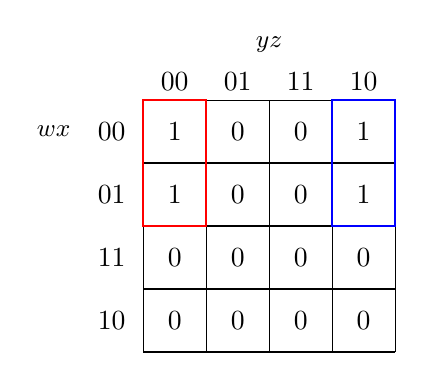
\begin{tikzpicture}[scale=0.8]
\draw (0,0) grid (4,4);
\node at (-0.5,3.5) {$00$}; \node at (-0.5,2.5) {$01$}; \node at (-0.5,1.5) {$11$}; \node at (-0.5,0.5) {$10$};
\node at (0.5,4.3) {$00$}; \node at (1.5,4.3) {$01$}; \node at (2.5,4.3) {$11$}; \node at (3.5,4.3) {$10$};
\node[left] at (-1,3.5) {\small $wx$};
\node[above] at (2,4.6) {\small $yz$};
\node at (0.5,3.5) {1}; \node at (1.5,3.5) {0}; \node at (2.5,3.5) {0}; \node at (3.5,3.5) {1};
\node at (0.5,2.5) {1}; \node at (1.5,2.5) {0}; \node at (2.5,2.5) {0}; \node at (3.5,2.5) {1};
\node at (0.5,1.5) {0}; \node at (1.5,1.5) {0}; \node at (2.5,1.5) {0}; \node at (3.5,1.5) {0};
\node at (0.5,0.5) {0}; \node at (1.5,0.5) {0}; \node at (2.5,0.5) {0}; \node at (3.5,0.5) {0};
\draw[thick,red] (0,2) rectangle (1,4);
\draw[thick,blue] (3,2) rectangle (4,4);
\end{tikzpicture}
\end{center}
\begin{center}
\small $4$-variable K-map: red block gives $\overline{x}\,\overline{y}\,\overline{z}$, blue block gives $\overline{x}yz$ -- both size-$2$ blocks (one variable eliminated each)
\end{center}

\begin{note}[Reading off blocks]
A block of size $2^k$ eliminates exactly $k$ variables from its minterm (the $k$ variables that differ across the block's cells); the surviving literals are read from whichever value ($0\to$negated, $1\to$plain) is constant across the whole block.
\end{note}

\begin{definition}[Don't-care condition]
An input combination that (by problem constraints) never actually occurs; marked `d' or `$\times$' on the K-map, and can be treated as either $0$ or $1$ -- whichever helps form a larger block.
\end{definition}

\bigskip
\begin{note}[Quine-McCluskey algorithm, Rosen -- harder, systematic alternative]
K-maps become impractical beyond $4$--$5$ variables (grids too large to draw/read visually). The \emph{Quine-McCluskey algorithm} systematizes the same idea.
\end{note}

\begin{algorithm}[H]
\SetAlgoLined
\KwIn{List of minterms as bit strings}
\KwOut{Set of prime implicants covering every minterm}
terms $\gets$ minterms, each unmarked\;
\While{some pair in terms differs in exactly one bit}{
    \ForEach{pair $(t_1,t_2)$ differing in exactly one bit}{
        mark $t_1,t_2$ as combined\;
        add $t_1$ with that bit replaced by ``--'' to newTerms\;
    }
    terms $\gets$ newTerms (duplicates removed)\;
}
primeImplicants $\gets$ all terms never marked combined\;
select a minimal subset of primeImplicants covering every original minterm (set-cover)\;
\Return{selected subset}\;
\caption{Quine-McCluskey algorithm}
\end{algorithm}

% ============================================================
% CHAPTER 5 --- PREDICATE LOGIC  (CN Ch.5, §5.1-5.15)
% ============================================================
\newpage
\section{Predicate Logic}

\subsection{Relations, predicates, and truth-valued functions}
\label{sec:5-1}
% CN 5.1 / Rosen 1.4

\begin{definition}[Predicate]
A \emph{predicate} is a relation (\S\ref{sec:2-13}, \S\ref{sec:2-17}), used with intent to do logic with it. A predicate with $k$ arguments is \emph{$k$-ary}.
\end{definition}

\begin{definition}[Predicate as a truth-valued function, Rosen]
A $k$-ary relation $R \subseteq A_1\times\cdots\times A_k$ can equivalently be viewed as a function
\[
R : A_1\times\cdots\times A_k \to \{T,F\}, \qquad R(a_1,\dots,a_k) = T \iff (a_1,\dots,a_k)\in R.
\]
Rosen also calls this a \emph{propositional function}.
\end{definition}

\begin{note}[Substitution yields a proposition]
Giving specific values to every argument of a predicate produces a proposition (definite truth value).
\end{note}

\begin{note}[Equality is always available]
$=$ is a predicate assumed available for \emph{every} domain -- without it, no domain of objects could even be meaningfully discussed.
\end{note}

\begin{definition}[Property]
A unary predicate (\emph{property}) $P(x)$ on domain $D$ corresponds to the set $\{x\in D : P(x)\}$.
\end{definition}

\subsection{Variables and constants}
\label{sec:5-2}
% CN 5.2 / Rosen 1.4

\begin{definition}[Variable]
A name for an object, without specifying it exactly, used to reason about an unknown or arbitrary member of its \emph{domain}.
\end{definition}

\begin{note}[Domain]
    $Domain$ also call $domain of discourse$ or $universe of discourse$.
\end{note}

\begin{definition}[Constant]
An object belonging to the domain of some variable -- a specific, named member of that domain.
\end{definition}

\begin{note}[Every variable has a domain]
E.g.\ ``let $x\in\Z$'' declares $x$ with domain $\Z$; a Boolean variable always has domain $\{T,F\}$.
\end{note}

\begin{note}[Math vs.\ programming variables, Rosen]
A programming variable occupies memory and is restricted to finite/representable values; a mathematical variable has no memory association and its domain may be infinite.
\end{note}

\subsection{Predicates and variables}
\label{sec:5-3}
% CN 5.3 / Rosen 1.4

\begin{definition}[Free variable]
A variable in a predicate expression not (yet) assigned a value.
\end{definition}

\begin{note}[Truth value requires all arguments fixed]
An expression with $\ge1$ free variable is not a proposition (no truth value). Only when \emph{every} free variable is assigned a value from its domain does the expression become a proposition.
\end{note}

\begin{note}[Domain matching is mandatory]
Any value or variable placed into an argument of a predicate must belong to that argument's declared domain -- mismatched domains make the expression ill-formed, not just false.
\end{note}

\begin{example}
$\mathrm{Parent}(\text{Alan Turing}, X)$ with $X$ a free variable, domain $\mathbb P$ (people): not a proposition. Substituting $X=$``Sara Turing'' gives the proposition $\mathrm{Parent}(\text{Alan Turing},\text{Sara Turing})$, true.
\end{example}

\begin{note}[Prefix vs.\ infix notation, Rosen]
Newly defined predicates typically use prefix notation, $R(a,b)$; predicates for ordering/equality/equivalence conventionally use infix notation, $a<b$, $a=b$ (\S\ref{sec:2-5}).
\end{note}

\subsection{Arguments of predicates}
\label{sec:5-4}
% CN 5.4

\begin{definition}[Term, recursive]
A \emph{term} of domain $D$ is one of:
\begin{itemize}
    \item a constant from $D$;
    \item a variable with domain $D$;
    \item a function with codomain $D$, each of whose arguments is given a term of matching domain.
\end{itemize}
\end{definition}

\begin{note}[Recursion bottoms out]
Terms are built from constants/variables/functions to arbitrary finite depth (composition, nested function calls), but never infinitely -- every term has a finite construction.
\end{note}

\begin{example}
Let $a,b$ be variables with domain $\R$. The expression
\[
a^2+b^2
\]
is a term of domain $\R$.

To see this, first consider $a^2$. The squaring function
\[
\operatorname{square}:\R\to\R
\]
has codomain $\R$, and its argument $a$ is a term of domain $\R$. Therefore,
\[
a^2=\operatorname{square}(a)
\]
is a term of domain $\R$.

Similarly, since $b$ is a term of domain $\R$,
\[
b^2=\operatorname{square}(b)
\]
is also a term of domain $\R$.

Finally, consider the real addition function
\[
+:\R\times\R\to\R.
\]
Its two arguments must each be terms of domain $\R$. Since both $a^2$ and $b^2$ are terms of domain $\R$, they can be given to the two arguments of the addition function. Hence,
\[
a^2+b^2
\]
is a term of domain $\R$.
\end{example}

\begin{example}
Let $\mathbb P$ be the domain of people, and suppose that
\[
\operatorname{FatherOf}:\mathbb P\to\mathbb P
\]
and
\[
\operatorname{MotherOf}:\mathbb P\to\mathbb P.
\]
If $Y$ is a variable with domain $\mathbb P$, then
\[
\operatorname{FatherOf}(Y)
\]
is a term of domain $\mathbb P$. Consequently,
\[
\operatorname{MotherOf}(\operatorname{FatherOf}(Y))
\]
is also a term of domain $\mathbb P$.
\end{example}

\begin{example}[Not terms]
$2+3+$ (malformed), $x{+}{+}$ (undefined operation here), $\log x$ (if $\log$ is not among the available functions), $z$ (if $z$ is neither a declared variable nor constant).
\end{example}

\begin{note}
Only terms whose domain matches an argument's declared domain may be plugged into that argument -- of a function \emph{or} a predicate; the same matching rule applies uniformly at every level of nesting.
\end{note}

\subsection{Building logical expressions with predicates}
\label{sec:5-5}
% CN 5.5 / Rosen 1.4

\begin{definition}[Predicate logic expression, recursive]
\begin{itemize}
    \item $T, F$ are predicate logic expressions.
    \item A predicate applied to terms of matching domains is a predicate logic expression.
    \item If $E,F$ are predicate logic expressions, so are $(E),\ \neg E,\ E\wedge F,\ E\vee F,\ E\implies F,\ E\iff F$.
\end{itemize}
\end{definition}

\begin{note}[Free variables propagate]
A predicate logic expression's free variables are the union of the free variables of its terms/sub-expressions -- combining expressions never removes a free variable (only quantification, \S\ref{sec:5-6}-5.9, does that).
\end{note}

\begin{example}
$(1<i)\wedge(i<n)$ has free variables $i,n$. $\mathrm{Parent}(X,Y)\iff\big(Y=\mathrm{MotherOf}(X)\big)\vee\big(Y=\mathrm{FatherOf}(X)\big)$ has free variables $X,Y$.
\end{example}

\begin{note}[Boolean algebra applies unchanged]
Every law from Chapter 4 (De Morgan's, distributive, etc.) applies to predicate logic expressions exactly as to propositions -- since fixing values for all free variables reduces any predicate expression to an ordinary proposition, and the laws hold for \emph{every} such assignment.
\end{note}

\subsection{Existential quantifier}
\label{sec:5-6}
% CN 5.6 / Rosen 1.4

\begin{definition}[Existential quantifier]
For predicate $P(x)$ on domain $D$:
\[
\exists x\, P(x)
\]
is true iff $P(a)$ is true for \emph{at least one} $a\in D$.
\end{definition}

\begin{note}[Punctuation]
$\exists x : P(x)$, $\exists x.\, P(x)$, $\exists x\, P(x)$ are all used; the colon/period is read ``such that''.
\end{note}

\begin{definition}[Bound variable]
Once quantified, $x$ is \emph{bound}: no longer available to receive a specific value. A fully-quantified expression has no free variables and is a genuine proposition, with a definite truth value.
\end{definition}

\begin{note}[Domain matters]
$\exists W\in\N:\ W<0$ is false; $\exists W\in\Z:\ W<0$ is true -- same predicate, different domain, different truth value.
\end{note}

\begin{note}[Analogy with disjunction -- and where it breaks]
$\exists x \in D,\ P(x)$ behaves like the disjunction $\bigvee_{a\in D} P(a)$ -- true iff at least one disjunct is true. But this is only an analogy: disjunctions must be \emph{finite}, while $D$ may be infinite, so existential quantification genuinely extends what propositional logic alone can express.
\end{note}

\begin{note}[Vacuous quantification]
If $x$ does not appear in $P$, $\exists x\, P$ is equivalent to $P$ itself (the quantifier is inert): e.g.\ $\exists w:\ z<0$ is just $z<0$.
\end{note}

\begin{note}
Quantifiers apply only to variables, never to constants: $\exists 5$ or $\exists\text{Annie}$ are ill-formed.
\end{note}

\bigskip
\begin{example}[Rosen -- harder: nested quantifiers and negation]
Let $P(x,y)$ mean ``$x+y=0$'' on domain $\R$. Consider $\exists x\, \forall y\, P(x,y)$ vs.\ $\forall y\, \exists x\, P(x,y)$.
\[
\exists x\, \forall y\, P(x,y): \text{one fixed } x \text{ that works for \emph{every} } y \text{ -- false (no single } x \text{ satisfies } x+y=0 \text{ for all } y\text{)}.
\]
\[
\forall y\, \exists x\, P(x,y): \text{for each } y, \text{ some } x \text{ (possibly depending on } y\text{) works -- true, take } x=-y.
\]
This shows quantifier \emph{order} genuinely matters -- covered fully in \S\ref{sec:5-10}.
\end{example}

\subsection{Restricting existentially quantified variables}
\label{sec:5-7}
% CN 5.7 / Rosen 1.4 (restricted quantifiers)

\begin{note}[Restricting $\exists$ uses $\wedge$]
To assert ``some $X$ satisfying $R(X)$ also satisfies $P(X)$'':
\[
\exists X:\ R(X) \wedge P(X).
\]
\end{note}

\begin{example}[Correct vs.\ a common wrong attempt]
``Some computer is human'':
\[
\text{correct: } \exists X:\ \mathrm{computer}(X)\wedge\mathrm{human}(X), \qquad
\text{wrong: } \exists X:\ \mathrm{computer}(X)\implies\mathrm{human}(X).
\]
The wrong version says ``something is not a computer, or is human'' -- true of any non-computer, regardless of computers at all, so it fails to capture the intended restriction.
\end{example}

\bigskip
\begin{note}[Rosen's restricted-quantifier shorthand]
Rosen writes $\exists X \in D\, [\dots]$ or $\exists X<0\, [\dots]$ directly as shorthand for the conjunction above, folding the restriction into the quantifier notation itself rather than writing it as an explicit $\wedge$.
\end{note}

\subsection{Universal quantifier}
\label{sec:5-8}
% CN 5.8 / Rosen 1.4

\begin{definition}[Universal quantifier]
For predicate $P(x)$ on domain $D$:
\[
\forall x\, P(x)
\]
is true iff $P(a)$ is true for \emph{every} $a\in D$.
\end{definition}

\begin{note}
As with $\exists$: the quantified variable becomes bound; an irrelevant quantifier (variable not appearing in the body) can be dropped.
\end{note}

\bigskip
\begin{note}[Rosen -- vacuous truth generalizes]
$\forall x\in\emptyset,\ P(x)$ is vacuously true for \emph{any} $P$, exactly generalizing $\emptyset\subseteq A$ (\S\ref{sec:1-6} Theorem 1) to arbitrary predicates, not just set membership.
\end{note}

\subsection{Restricting universally quantified variables}
\label{sec:5-9}
% CN 5.9 / Rosen 1.4

\begin{note}[Restricting $\forall$ uses $\implies$]
To assert ``every $X$ satisfying $R(X)$ also satisfies $P(X)$'':
\[
\forall X:\ R(X) \implies P(X).
\]
\end{note}

\begin{example}[Correct vs.\ a common wrong attempt]
``Every computer is human'':
\[
\text{correct: } \forall X:\ \mathrm{computer}(X)\implies\mathrm{human}(X), \qquad
\text{wrong: } \forall X:\ \mathrm{computer}(X)\wedge\mathrm{human}(X).
\]
The wrong version says ``everything is both a computer and human'' -- forces non-computers to also be human computers, which was never intended.
\end{example}

\begin{note}[The mirror-image trap, worth memorizing]
$\exists$ pairs naturally with $\wedge$; $\forall$ pairs naturally with $\implies$. Swapping these (using $\implies$ with $\exists$, or $\wedge$ with $\forall$) is one of the most common predicate-logic errors -- always double check which connective a restricted quantifier needs.
\end{note}

\bigskip
\begin{theorem}[De Morgan's for quantifiers, Rosen -- preview of \S\ref{sec:5-13}]
\[
\neg\forall x\, P(x) \ \equiv\ \exists x\,\neg P(x), \qquad \neg\exists x\, P(x) \ \equiv\ \forall x\,\neg P(x).
\]
\end{theorem}
\begin{note}
Consequence: negating $\forall X: R(X)\implies P(X)$ gives $\exists X: R(X)\wedge\neg P(X)$ -- exactly matching the $\exists/\wedge$ pairing above, since $\neg(R\implies P) \equiv R\wedge\neg P$ (\S\ref{sec:4-15}).
\end{note}

\subsection{Multiple quantifiers}
\label{sec:5-10}
% CN 5.10 / Rosen 1.4

\begin{note}[Same-type quantifiers commute]
\[
\exists X\,\exists Y\, P = \exists Y\,\exists X\, P = \exists(X,Y)\, P, \qquad
\forall X\,\forall Y\, P = \forall Y\,\forall X\, P = \forall(X,Y)\, P.
\]
\end{note}

\begin{note}[Mixed quantifiers do \emph{not} commute]
\[
\exists X\,\forall Y\, P, \quad \forall X\,\exists Y\, P, \quad \exists Y\,\forall X\, P, \quad \forall Y\,\exists X\, P
\]
are, in general, four genuinely different statements.
\end{note}

\begin{example}[hasVisited$(P,C)$: person $P$ has visited country $C$]
\[
\exists P\,\forall C:\ \text{someone has visited every country}, \qquad
\forall C\,\exists P:\ \text{every country has been visited by someone}.
\]
The first is a strong claim about one exceptional traveler; the second is far weaker (each country just needs \emph{some} visitor, possibly a different one each time).
\end{example}

\bigskip
\begin{example}[Rosen -- classic order-matters example]
Let $D(x,y)$ mean ``$x$ has dated $y$'' on the domain of all people.
\[
\exists x\,\forall y\, D(x,y): \text{someone has dated everyone}.
\]
\[
\forall y\,\exists x\, D(x,y): \text{everyone has been dated by someone.}
\]
The first implies the second (that one exceptional dater witnesses every $y$), but not conversely -- the second only needs, for each $y$, \emph{some} $x$, possibly different for each $y$.
\end{example}

\begin{theorem}[$\exists\forall \implies \forall\exists$, general fact, Rosen]
\[
\exists x\,\forall y\, P(x,y) \ \implies\ \forall y\,\exists x\, P(x,y).
\]
The converse implication does \emph{not} hold in general.
\end{theorem}
\begin{proof}
Suppose $\exists x\,\forall y\,P(x,y)$: fix such an $x_0$, so $P(x_0,y)$ holds for every $y$. Then for any $y$, taking $x=x_0$ witnesses $\exists x\,P(x,y)$ -- so $\forall y\,\exists x\,P(x,y)$ holds. The dating example above (with $D$ not symmetric enough to reverse) shows the converse can fail.
\end{proof}

\paragraph{Quantifier--connective pitfall.***} $\forall$ pairs with
$\Rightarrow$; $\exists$ pairs with $\wedge$ --- the other way round
lets a trivial witness make the statement true for the wrong reason.

\subsection{Predicate logic expressions}
\label{sec:5-11}
% CN 5.11 / Rosen 1.4

\begin{definition}[Predicate logic expression, complete recursive grammar]
\begin{itemize}
    \item $T,F$ are predicate logic expressions.
    \item Terms of matching domains plugged into a predicate give a predicate logic expression.
    \item If $E,F$ are predicate logic expressions: $(E),\ \neg E,\ E\wedge F,\ E\vee F,\ E\implies F,\ E\iff F$.
    \item If $E$ is a predicate logic expression and $X$ is a free variable of $E$: $\exists X: E$ and $\forall X: E$ are predicate logic expressions, and $X$ is \emph{no longer free} in either.
\end{itemize}
\end{definition}

\begin{note}[Free variables shrink under quantification]
If $V$ is the free-variable set of $E$, then $\exists X: E$ and $\forall X: E$ each have free-variable set $V\setminus\{X\}$.
\end{note}

\subsection{Doing logic with quantifiers}
\label{sec:5-12}
% CN 5.12 / Rosen 1.4

\begin{note}[Instantiation and generalization]
\[
\big(\forall X\, P(X)\big) \implies P(\mathrm{obj}), \qquad P(\mathrm{obj}) \implies \big(\exists X\, P(X)\big)
\]
for any specific $\mathrm{obj}$ in $X$'s domain.
\end{note}

\begin{theorem}[$\forall$ distributes over $\wedge$; $\exists$ distributes over $\vee$]
\[
\forall X\,(P(X)\wedge Q(X)) \ \equiv\ (\forall X\, P(X)) \wedge (\forall X\, Q(X)),
\]
\[
\exists X\,(P(X)\vee Q(X)) \ \equiv\ (\exists X\, P(X)) \vee (\exists X\, Q(X)).
\]
\end{theorem}

\begin{note}[$\forall$ over $\vee$, and $\exists$ over $\wedge$, only give one-way implications, Rosen]
\[
(\forall X\, P(X)) \vee (\forall X\, Q(X)) \implies \forall X\,(P(X)\vee Q(X)),
\]
\[
\exists X\,(P(X)\wedge Q(X)) \implies (\exists X\, P(X)) \wedge (\exists X\, Q(X)),
\]
but neither converse holds in general -- e.g.\ every integer is even or odd ($\forall X$, $\mathrm{even}(X)\vee\mathrm{odd}(X)$), yet it is false that every integer is even, or every integer is odd.
\end{note}

\begin{definition}[Scope of a quantified variable]
The sub-expression from the quantifier to the end of its innermost enclosing parentheses (or the end of the whole expression, if unparenthesized).
\end{definition}

\begin{example}[Two disjoint scopes, same variable name]
In $(\forall X\, P(X)) \wedge (\forall X\, Q(X))$, the two $X$'s are entirely independent -- like distinct local variables in a program that happen to share a name.
\end{example}

\paragraph{At least / at most / exactly $n$ (predicate logic).}
At least $n$:
\[
\exists x_1\cdots x_n\Big(\bigwedge_{i<j}x_i\neq x_j \wedge \bigwedge_i P(x_i)\Big)
\]
At most $n$:
\[
\forall x_1\cdots x_{n+1}\Big(\bigwedge_i P(x_i)\Rightarrow \bigvee_{i<j}x_i=x_j\Big)
\]
Exactly $n$: conjunction of both.

\paragraph{The uniqueness quantifier $\exists!$.} $\exists!\,x\,P(x)$
means ``there is a unique $x$ such that $P(x)$.'' Without ``$!$'':
\[
\exists!\,x\,P(x) \;\equiv\; \exists x\,\Big(P(x)\wedge\forall z\big(P(z)\Rightarrow z=x\big)\Big)
\]
General template for ``exactly one thing satisfies $P$'':
existence ($P(x)$) $\wedge$ uniqueness (anything satisfying $P$
equals $x$). \emph{(CN Ch.5 Problem 4; Rosen \S1.5 Ex.\ 52.)}

\subsection{Duality between quantifiers}
\label{sec:5-13}
% CN 5.13 / Rosen 1.4 (De Morgan's laws for quantifiers)

\begin{theorem}[De Morgan's laws for quantifiers]
\[
\neg\forall X\, P(X) \ \equiv\ \exists X\,\neg P(X), \qquad \neg\exists X\, P(X) \ \equiv\ \forall X\,\neg P(X).
\]
\end{theorem}

\begin{example}[``Not all stars are visible'' $=$ ``some star is invisible'']
\begin{align*}
\neg\forall X\,(\mathrm{star}(X)\implies\mathrm{visible}(X))
&= \exists X\,\neg(\mathrm{star}(X)\implies\mathrm{visible}(X)) \\
&= \exists X\,\neg(\neg\mathrm{star}(X)\vee\mathrm{visible}(X)) \\
&= \exists X\,(\mathrm{star}(X)\wedge\neg\mathrm{visible}(X)).
\end{align*}
\end{example}

\begin{note}
$\neg\forall Y\,\neg = \exists Y$, and $\neg\exists Y\,\neg = \forall Y$ (apply the laws twice, using double negation).
\end{note}

\subsection{Some examples}
\label{sec:5-15}
% CN 5.15 / Rosen 1.4

\begin{example}[``Infinitely many primes'', in predicate logic]
With $\mathrm{Prime}(n)$ on domain $\N$ and predicate $\le$:
\[
\forall b\, \exists n\ \mathrm{Prime}(n) \wedge \neg(n \le b).
\]
Read: for every bound $b$, some prime exceeds it -- correctly capturing ``infinitely many primes'' without needing an infinite conjunction.
\end{example}

\begin{example}[Swapping the quantifiers gives a different, false, statement]
\[
\exists n\, \forall b\ \mathrm{Prime}(n) \wedge \neg(n \le b).
\]
\end{example}
\begin{proof}[Why this is false -- step by step]
Distribute $\forall b$ over the conjunction (\S\ref{sec:5-12}):
\[
\forall b\ \mathrm{Prime}(n) \wedge \neg(n\le b) \ \equiv\ (\forall b\, \mathrm{Prime}(n)) \wedge (\forall b\, \neg(n\le b)).
\]

Since $\mathrm{Prime}(n)$ does not involve $b$, the quantifier is superfluous (\S\ref{sec:5-9}):
\[
\forall b\, \mathrm{Prime}(n) \ \equiv\ \mathrm{Prime}(n).
\]

Substituting back:
\[
\exists n\,\big(\mathrm{Prime}(n) \wedge \forall b\,\neg(n\le b)\big) \ \equiv\ \exists n\in\{\text{primes}\}\ \forall b\ n>b.
\]

This asserts a single prime exceeding \emph{every} number -- false. So the two quantifier orderings genuinely differ in meaning, one true and one false.
\end{proof}

\bigskip
\begin{example}[Rosen -- translating a nested-quantifier English sentence, harder]
``Every real number except $0$ has a multiplicative inverse.'' With $\mathrm{domain}=\R$:
\[
\forall x\,\big(x\neq 0 \implies \exists y\, (xy=1)\big).
\]
Note the restricted-$\forall$ pattern from \S\ref{sec:5-9} ($x\neq0 \implies \cdots$) nested with a plain $\exists y$ inside -- $y$'s existence is allowed to depend on $x$, which is essential: no single $y$ works for every nonzero $x$.
\end{example}

\bigskip
\begin{example}[Limit of a function, nested quantifiers -- Rosen, requires calculus]
$\lim_{x\to a} f(x) = L$ means: for every real number $\epsilon>0$ there exists a real number $\delta>0$ such that $|f(x)-L|<\epsilon$ whenever $0<|x-a|<\delta$.

In quantifiers, with $\epsilon,\delta$ ranging over \emph{all} reals and the positivity built into the body:
\[
\forall\epsilon\,\exists\delta\,\forall x\,\Big(0<|x-a|<\delta \implies |f(x)-L|<\epsilon\Big),
\]
where the domain for $\epsilon,\delta$ is understood to already be ``positive reals,'' and for $x$ is all reals.

Equivalently, using \emph{restricted} quantifiers (\S\ref{sec:5-7}, \S\ref{sec:5-9}) to make the positivity explicit rather than implicit in the domain:
\[
\forall\epsilon>0\,\exists\delta>0\,\forall x\,\Big(0<|x-a|<\delta \implies |f(x)-L|<\epsilon\Big),
\]
now with $\epsilon,\delta$ ranging over \emph{all} real numbers, and the restriction ``$>0$'' carried by the quantifier notation itself instead of by the choice of domain.
\end{example}

\begin{note}[Order is essential here]
The quantifier order $\forall\epsilon\,\exists\delta\,\forall x$ matters critically: $\delta$ is allowed to depend on $\epsilon$ (chosen \emph{after} $\epsilon$ is fixed), but must work for \emph{all} $x$ satisfying the closeness condition. Swapping to $\exists\delta\,\forall\epsilon$ would wrongly demand a single $\delta$ working for every $\epsilon$ simultaneously -- a much stronger, generally false, claim.
\end{note}

\bigskip
\begin{example}[``Limit does not exist,'' via negation of nested quantifiers -- Rosen, requires calculus]
$\lim_{x\to a} f(x)$ does not exist means: for every real number $L$, $\lim_{x\to a}f(x)\neq L$.

Using the restricted-quantifier form above, $\lim_{x\to a}f(x)\neq L$ is the negation of
\[
\forall\epsilon>0\,\exists\delta>0\,\forall x\,\Big(0<|x-a|<\delta \implies |f(x)-L|<\epsilon\Big),
\]
i.e.
\[
\neg\forall\epsilon>0\,\exists\delta>0\,\forall x\,\Big(0<|x-a|<\delta \implies |f(x)-L|<\epsilon\Big).
\]

Push the negation inward one quantifier at a time, using \S\ref{sec:5-13}'s De Morgan's laws for quantifiers at each step:
\begin{align*}
&\phantom{{}\equiv{}} \neg\forall\epsilon>0\,\exists\delta>0\,\forall x\,(0<|x-a|<\delta\implies|f(x)-L|<\epsilon) \\
&\equiv \exists\epsilon>0\,\neg\exists\delta>0\,\forall x\,(0<|x-a|<\delta\implies|f(x)-L|<\epsilon) \\
&\equiv \exists\epsilon>0\,\forall\delta>0\,\neg\forall x\,(0<|x-a|<\delta\implies|f(x)-L|<\epsilon) \\
&\equiv \exists\epsilon>0\,\forall\delta>0\,\exists x\,\neg\big(0<|x-a|<\delta\implies|f(x)-L|<\epsilon\big) \\
&\equiv \exists\epsilon>0\,\forall\delta>0\,\exists x\,\Big(0<|x-a|<\delta \ \wedge\ |f(x)-L|\ge\epsilon\Big).
\end{align*}
The last step uses $\neg(P\implies Q)\equiv P\wedge\neg Q$ (\S\ref{sec:4-15}), applied with $P=(0<|x-a|<\delta)$, $Q=(|f(x)-L|<\epsilon)$, and $\neg(|f(x)-L|<\epsilon) \equiv |f(x)-L|\ge\epsilon$.

Since ``the limit does not exist'' means $\forall L$, $\lim_{x\to a}f(x)\neq L$, prepend $\forall L$:
\[
\forall L\,\exists\epsilon>0\,\forall\delta>0\,\exists x\,\Big(0<|x-a|<\delta \ \wedge\ |f(x)-L|\ge\epsilon\Big).
\]

Read aloud: ``for every candidate limit value $L$, there is some $\epsilon>0$ such that, no matter how small a $\delta>0$ is chosen, some $x$ within $\delta$ of $a$ still has $f(x)$ at least $\epsilon$ away from $L$'' -- exactly capturing that no $L$ can serve as the limit.
\end{example}

\begin{note}
Each of the four inner negation steps flips $\forall\leftrightarrow\exists$ and pushes $\neg$ past exactly one quantifier, mirroring the definitions in \S\ref{sec:5-13} one at a time; only the final step differs, converting the negated implication via ordinary propositional logic rather than a quantifier law.
\end{note}

\bigskip
\begin{example}[Negating a triple-nested quantifier statement -- Rosen, harder]
``There is no woman who has flown on every airline in the world.'' Let $P(w,f)$: ``woman $w$ has taken flight $f$''; $Q(f,a)$: ``flight $f$ is on airline $a$.'' ``Some woman has flown on every airline'' is
\[
\exists w\,\forall a\,\exists f\,\big(P(w,f)\wedge Q(f,a)\big),
\]
so the negation is $\neg\exists w\,\forall a\,\exists f\,(P(w,f)\wedge Q(f,a))$. Pushing the negation inward, one quantifier at a time:
\begin{align*}
&\phantom{{}\equiv{}} \neg\exists w\,\forall a\,\exists f\,(P(w,f)\wedge Q(f,a)) \\
&\equiv \forall w\,\neg\forall a\,\exists f\,(P(w,f)\wedge Q(f,a)) \\
&\equiv \forall w\,\exists a\,\neg\exists f\,(P(w,f)\wedge Q(f,a)) \\
&\equiv \forall w\,\exists a\,\forall f\,\neg(P(w,f)\wedge Q(f,a)) \\
&\equiv \forall w\,\exists a\,\forall f\,\big(\neg P(w,f)\vee\neg Q(f,a)\big).
\end{align*}
Reading it back: ``for every woman, there is some airline such that, for every flight, either she hasn't taken that flight or that flight isn't on that airline.''
\end{example}

\begin{note}
Three nested quantifiers, three applications of the same rule from \S\ref{sec:5-13} -- the pattern doesn't change with depth, only the bookkeeping does.
\end{note}

\subsection{Summary of rules for logic with quantifiers}
\label{sec:5-14}
% CN 5.14

\begin{note}[Full rule list]
\begin{align*}
\exists x\in A\, P(x) &\equiv \exists x\,(x\in A \wedge P(x)) & \text{(\S\ref{sec:5-7})}\\
\forall x\in A\, P(x) &\equiv \forall x\,(x\in A \implies P(x)) & \text{(\S\ref{sec:5-9})}\\
\exists x\, R &\equiv R, \quad \forall x\, R \equiv R & (x \text{ not free in } R;\ \S\ref{sec:5-7},5.9)\\
\exists x\exists y\, P(x,y) &\equiv \exists y\exists x\, P(x,y) & \text{(\S\ref{sec:5-10})}\\
\forall x\forall y\, P(x,y) &\equiv \forall y\forall x\, P(x,y) & \text{(\S\ref{sec:5-10})}\\
\forall x\, P(x) &\implies P(\mathrm{obj}), \quad P(\mathrm{obj}) \implies \exists x\, P(x) & \text{(\S\ref{sec:5-12})}\\
\exists x\,(P(x)\vee Q(x)) &\equiv (\exists x\,P(x))\vee(\exists x\,Q(x)) & \text{(\S\ref{sec:5-12})}\\
\forall x\,(P(x)\wedge Q(x)) &\equiv (\forall x\,P(x))\wedge(\forall x\,Q(x)) & \text{(\S\ref{sec:5-12})}\\
\neg\exists x\, P(x) &\equiv \forall x\,\neg P(x), \quad \neg\forall x\, P(x) \equiv \exists x\,\neg P(x) & \text{(\S\ref{sec:5-13})}
\end{align*}
\end{note}

\subsection{Rules of inference (Rosen \S\ref{sec:1-6} -- extension, beyond CN syllabus)}

\begin{definition}[Rule of inference]
A \emph{rule of inference} is an argument form: premises above a line, conclusion below, valid because the conjunction of the premises implying the conclusion is a tautology.
\end{definition}

\begin{note}[Basic rules for propositional logic]
\[
\text{Modus ponens: } \frac{P,\ P\implies Q}{\therefore Q}
\qquad
\text{Modus tollens: } \frac{\neg Q,\ P\implies Q}{\therefore \neg P}
\]
\[
\text{Hypothetical syllogism: } \frac{P\implies Q,\ Q\implies R}{\therefore P\implies R}
\qquad
\text{Disjunctive syllogism: } \frac{P\vee Q,\ \neg P}{\therefore Q}
\]
\[
\text{Addition: } \frac{P}{\therefore P\vee Q}
\qquad
\text{Simplification: } \frac{P\wedge Q}{\therefore P}
\qquad
\text{Conjunction: } \frac{P,\ Q}{\therefore P\wedge Q}
\]
\[
\text{Resolution: } \frac{P\vee Q,\ \neg P\vee R}{\therefore Q\vee R}
\]
\end{note}

\begin{theorem}
Each rule above is valid: the conjunction of its premises implies its conclusion is a tautology.
\end{theorem}
\begin{proof}[Verification for modus tollens]
Suppose $\neg Q$ and $P\implies Q$ both hold. If $P$ were true, $P\implies Q$ would force $Q$ true, contradicting $\neg Q$. So $P$ is false, i.e.\ $\neg P$ holds. (The others verify similarly, by truth table or direct argument -- \S\ref{sec:4-15}'s laws are exactly what's needed.)
\end{proof}

\bigskip
\begin{note}[Rules of inference for quantified statements]
\[
\text{Universal instantiation: } \frac{\forall x\, P(x)}{\therefore P(c)} \ (c \text{ any specific element of the domain})
\]
\[
\text{Universal generalization: } \frac{P(c) \text{ for arbitrary, generic } c}{\therefore \forall x\, P(x)}
\]
\[
\text{Existential instantiation: } \frac{\exists x\, P(x)}{\therefore P(c)} \ (c \text{ some element, not otherwise specified})
\]
\[
\text{Existential generalization: } \frac{P(c) \text{ for a specific } c}{\therefore \exists x\, P(x)}
\]
\end{note}

\begin{note}[These match CN's own principles]
Universal instantiation and existential generalization are exactly the two implications from \S\ref{sec:5-12}; universal generalization is exactly the ``let $x$ be arbitrary, generic'' technique from \S\ref{sec:3-3}/\S\ref{sec:3-4} for proving universal statements.
\end{note}

\bigskip
\begin{example}[Chained formal proof -- harder, Rosen-style]
Premises: (1) $\forall x\,(\mathrm{Student}(x)\implies\mathrm{Studies}(x))$; (2) $\forall x\,(\mathrm{Studies}(x)\implies\mathrm{Passes}(x))$; (3) $\neg\mathrm{Passes}(\text{Sam})$; (4) $\mathrm{Student}(\text{Sam})$.

Conclusion to derive: a contradiction (showing the premises are jointly unsatisfiable).

\begin{enumerate}[label=(\arabic*)]
    \setcounter{enumi}{4}
    \item $\mathrm{Student}(\text{Sam})\implies\mathrm{Studies}(\text{Sam})$ \hfill (universal instantiation on (1), $c=$ Sam)
    \item $\mathrm{Studies}(\text{Sam})\implies\mathrm{Passes}(\text{Sam})$ \hfill (universal instantiation on (2), $c=$ Sam)
    \item $\mathrm{Student}(\text{Sam})\implies\mathrm{Passes}(\text{Sam})$ \hfill (hypothetical syllogism, (5)+(6))
    \item $\mathrm{Passes}(\text{Sam})$ \hfill (modus ponens, (4)+(7))
    \item $\mathrm{Passes}(\text{Sam}) \wedge \neg\mathrm{Passes}(\text{Sam})$ \hfill (conjunction, (8)+(3))
\end{enumerate}
Line (9) is a contradiction, so the four premises cannot all hold simultaneously.
\end{example}

% ============================================================
% CHAPTER 6 --- SEQUENCES & SERIES  (CN Ch.6, §6.1-6.16)
% ============================================================
\newpage
\section{Sequences \& Series}

\subsection{Definitions and notation}
\label{sec:6-1}
% CN 6.1 / Rosen 2.4

\begin{definition}[Sequence]
A \emph{sequence} is a function whose domain is $\N$ (an \emph{infinite sequence}) or $\{1,\dots,n\}$ for some $n$ (a \emph{finite sequence}, equivalently an ordered $n$-tuple, \S\ref{sec:1-14}).
\end{definition}

\begin{definition}[Term, $n$-th term notation]
For a sequence $f$ over a set $A$ (i.e.\ $f:\N\to A$ or similar), $f(n)$ (also written $f_n$) is the \emph{$n$-th term}. The \emph{terms} of $f$ are the members of its image (\S\ref{sec:2-1-2}), listed in the order given by the domain.
\end{definition}

\begin{definition}[Length]
The \emph{length} of a finite sequence is the size of its domain -- its number of terms.
\end{definition}

\begin{note}[Rosen's phrasing]
Rosen defines a sequence identically: a function from a subset of $\Z$ (typically $\{0,1,2,\dots\}$ or $\{1,2,3,\dots\}$) to a set $S$; $a_n$ denotes the image of $n$, called a \emph{term}.
\end{note}

\begin{note}[Ways to specify a sequence]
\begin{itemize}
    \item List all terms explicitly (only practical if short).
    \item A formula for the $n$-th term: $(n^2 : n\in\N)$ or $(n^2)_{n=1}^{\infty}$, matching set-builder notation (\S\ref{sec:1-2}) but with parentheses since order matters.
    \item A recurrence relation (\S\ref{sec:6-2}): each term defined using previous term(s).
\end{itemize}
A sequence is \emph{not} well-defined merely by listing a few terms and trusting a "pattern" -- infinitely many different formulas can match any finite initial segment (see \S\ref{sec:6-2}'s exercise on this danger, and the counterexample below).
\end{note}

\begin{example}[A pattern-guessing trap, Rosen -- harder]
The sequence $1,2,4,8,16,\dots$ (five terms shown) matches $a_n = 2^{n-1}$ -- but it also matches
\[
a_n = \binom{n-1}{0}+\binom{n-1}{1}+\binom{n-1}{2}+\binom{n-1}{3}+\binom{n-1}{4},
\]
which equals $1,2,4,8,16$ for $n=1,\dots,5$ but gives $31$, not $32$, at $n=6$ (since the $\binom{n-1}{5}$ term, absent from this formula, would otherwise contribute). A finite list of terms never uniquely determines a sequence.
\end{example}

\begin{note}[Number sequences]
Sequences over $\N,\Z,\Q,\R$ (\emph{number sequences}) are especially important -- not only for direct computation, but for measuring properties of computation itself: running time, memory use, input/output size, and so on.
\end{note}

\subsection{Recursive definitions of sequences}
\label{sec:6-2}
% CN 6.2 / Rosen 2.4, 5.3

\begin{definition}[Recurrence relation]
A \emph{recurrence relation} for $(a_n)$ expresses $a_n$ in terms of one or more earlier terms ($a_{n-1}$, or several), together with enough \emph{base cases} (initial terms given explicitly) to make every term uniquely determined.
\end{definition}

\begin{note}[General shape of a recursive definition, Rosen \S\ref{sec:5-3}]
\begin{itemize}
    \item \textbf{Base case}: explicitly define finitely many of the simplest objects.
    \item \textbf{Recursive case}: define a general object in terms of simpler ones already in the family.
\end{itemize}
This is the same two-part shape as recursively-defined sets/functions (\S\ref{sec:5-3} generalizes it beyond sequences -- see the note below).
\end{note}

\begin{example}
\[
f_1=1,\ f_n=f_{n-1}+2 \quad\Rightarrow\quad 1,3,5,7,\dots \text{ (odd numbers)};
\]
\[
f_1=0,\ f_n=f_{n-1}+2 \quad\Rightarrow\quad 0,2,4,6,\dots \text{ (even numbers)} \text{ -- same rule, different base case, different sequence};
\]
\[
f_1=1,\ f_n=nf_{n-1} \quad\Rightarrow\quad 1,2,6,24,120,\dots \text{ (factorials, i.e.\ } n!\text{)}.
\]
\end{example}

\begin{note}[Multiple base cases]
$f_n=4f_{n-2}$ (depending on the term \emph{two} back) needs \emph{two} base cases, $f_1,f_2$, to determine the whole sequence -- one base case alone only fixes every other term. E.g.\ $f_1=2,f_2=0,\ f_n=4f_{n-2}$ gives $2,0,8,0,32,0,\dots$
\end{note}

\bigskip
\begin{example}[Structural induction preview, Rosen \S\ref{sec:5-3} -- harder]
Recursively-defined \emph{sets} follow the same base/recursive pattern: e.g.\ the set $S$ of "balanced parenthesis strings" is defined by (i) $\varepsilon\in S$ (base case); (ii) if $w\in S$, then $(w)\in S$ and, if $u,v\in S$, then $uv\in S$ (recursive case). Proving a property $P$ holds for every $w\in S$ then uses \emph{structural induction}: prove $P$ for the base case, and prove that the recursive case preserves $P$ (assuming it holds for the smaller pieces used to build $w$) -- the direct set-theoretic analogue of induction on sequences.
\end{example}

\subsection{Arithmetic sequences}
\label{sec:6-3}
% CN 6.3 / Rosen 2.4

\begin{definition}[Arithmetic sequence]
A sequence with constant difference $d$ between consecutive terms: $f_1=a,\ f_n=f_{n-1}+d$. The $n$-th term is $a+(n-1)d$.
\end{definition}

\begin{note}[Rosen's phrasing]
Rosen calls this an \emph{arithmetic progression}: $a_n=a+dn$ (indexing from $n=0$) or equivalently $a_n=a_{n-1}+d$ -- same sequence, differing only in whether the first term is indexed $0$ or $1$.
\end{note}

\subsection{Geometric sequences}
\label{sec:6-4}
% CN 6.4 / Rosen 2.4

\begin{definition}[Geometric sequence]
A sequence with constant ratio $r$ between consecutive terms: $f_1=a,\ f_n=f_{n-1}\cdot r$. The $n$-th term is $ar^{n-1}$.
\end{definition}

\begin{note}[Rosen's phrasing]
Rosen calls this a \emph{geometric progression}: $a_n=ar^n$ (indexing from $0$) or $a_n=a_{n-1}\cdot r$.
\end{note}

\subsection{Harmonic sequences}
\label{sec:6-5}
% CN 6.5 -- no direct Rosen counterpart

\begin{definition}[Harmonic sequence]
$(a_n)$ is \emph{harmonic} iff $(1/a_n)$ is arithmetic.
\end{definition}

\begin{note}
$(1/n : n\in\N)$ is the key example -- harmonic since $\N$ itself is arithmetic. See \S\ref{sec:6-15} for its properties.
\end{note}

\subsection{From recursive definitions to formulas}
\label{sec:6-6}
% CN 6.6 / Rosen 8.1-8.2

\begin{note}[Explore -- conjecture -- prove]
\begin{enumerate}[label=\arabic*.]
    \item \textbf{Explore}: compute the first several terms.
    \item \textbf{Conjecture}: look for a pattern; propose a closed-form formula.
    \item \textbf{Prove}: verify the formula for all $n$, typically by induction.
\end{enumerate}
\end{note}

\begin{example}
\[
f_1=1,\quad f_n = 2f_{n-1}+1.
\]

\textbf{Explore}: $f_1=1,\ f_2=3,\ f_3=7,\ f_4=15$.

\textbf{Conjecture}: each term is one less than a power of $2$: $f_n = 2^n-1$.

\textbf{Prove} (induction on $n$):

\textit{Base case} ($n=1$): $2^1-1=1=f_1$.

\textit{Inductive step}: assume $f_k=2^k-1$ for some $k\ge1$. Then
\[
f_{k+1} = 2f_k+1 = 2(2^k-1)+1 = 2^{k+1}-2+1 = 2^{k+1}-1.
\]

By induction, $f_n=2^n-1$ for all $n\ge1$.
\end{example}

\bigskip
\begin{definition}[Linear homogeneous recurrence with constant coefficients, Rosen \S8.2 -- systematic method]
\[
a_n = c_1a_{n-1}+c_2a_{n-2}+\cdots+c_ka_{n-k}, \qquad c_k \neq 0,
\]
with $k$ initial conditions $a_0,\dots,a_{k-1}$ given. Its \emph{characteristic equation} is
\[
x^k - c_1x^{k-1}-c_2x^{k-2}-\cdots-c_k = 0.
\]
\end{definition}

\begin{theorem}[Distinct roots case, Rosen]
If the characteristic equation has $k$ \emph{distinct} roots $r_1,\dots,r_k$, then every solution has the form
\[
a_n = \alpha_1 r_1^n + \alpha_2 r_2^n + \cdots + \alpha_k r_k^n
\]
for constants $\alpha_1,\dots,\alpha_k$ determined by the initial conditions.
\end{theorem}
\begin{note}[Why this is really linear algebra]
The set of all sequences satisfying this recurrence forms a vector space: if $(b_n)$ and $(c_n)$ both satisfy it, so does any combination $\beta b_n+\gamma c_n$ (the recurrence is \emph{linear}). This space has dimension $k$ -- a solution is pinned down entirely by its $k$ initial values $a_0,\dots,a_{k-1}$.

Each geometric sequence $r_i^n$ is itself a solution (plugging it into the recurrence and using $r_i^k=c_1r_i^{k-1}+\cdots+c_k$ confirms it). When the $r_i$ are distinct, these $k$ solutions are \emph{linearly independent} -- this is exactly a Vandermonde-determinant fact from linear algebra: distinct roots $\Rightarrow$ nonzero Vandermonde determinant $\Rightarrow$ independence. $k$ independent vectors in a $k$-dimensional space form a \emph{basis}, so every solution is a unique linear combination of them -- which is exactly the formula above, with $\alpha_1,\dots,\alpha_k$ solved for using whatever initial conditions are given.
\end{note}

\begin{example}[Solving a second-order recurrence -- harder, worked example]
\[
a_n = 5a_{n-1} - 6a_{n-2}, \qquad a_0=1,\ a_1=4.
\]

\textbf{Characteristic equation}: $x^2-5x+6=0$, i.e.\ $(x-2)(x-3)=0$, roots $r_1=2,\ r_2=3$.

\textbf{General solution}: $a_n = \alpha_1 2^n + \alpha_2 3^n$.

\textbf{Solve for $\alpha_1,\alpha_2$} using initial conditions:
\[
a_0=1:\ \alpha_1+\alpha_2=1, \qquad a_1=4:\ 2\alpha_1+3\alpha_2=4.
\]
From the first equation, $\alpha_1=1-\alpha_2$; substituting: $2(1-\alpha_2)+3\alpha_2=4 \Rightarrow \alpha_2=2,\ \alpha_1=-1$.

\textbf{Closed form}:
\[
a_n = -2^n + 2\cdot3^n.
\]
\end{example}

\begin{note}[Why this beats guess-and-check]
The explore-conjecture-prove method above needs a pattern to be \emph{visible} in the first few terms -- it can fail entirely on recurrences with less obvious closed forms (this one, $a_n=5a_{n-1}-6a_{n-2}$, produces $1,4,14,46,\dots$, no obvious pattern by inspection). The characteristic-equation method is systematic: it always works, whenever the roots can be found. This is exactly the machinery behind the exact Fibonacci formula in \S\ref{sec:6-7-4}.
\end{note}

\bigskip
\begin{definition}[Recursively defined set, Rosen \S\ref{sec:5-3}]
A set $S$ is defined recursively by:
\begin{itemize}
    \item \textbf{Basis step}: specify an initial collection of elements in $S$.
    \item \textbf{Recursive step}: rules that construct new elements of $S$ from existing ones.
    \item (Implicitly) $S$ contains \emph{only} elements obtainable this way.
\end{itemize}
\end{definition}

\begin{example}[Balanced parenthesis strings]
Define $B$ recursively: (i) $\varepsilon\in B$ (empty string); (ii) if $w\in B$, then $(w)\in B$; (iii) if $u,v\in B$, then $uv\in B$.
\end{example}

\begin{definition}[Recursively defined function, Rosen \S\ref{sec:5-3}]
A function $f$ on a recursively defined set $S$ is defined by: giving $f$'s value(s) on the basis elements, and giving a rule for $f$'s value on a constructed element in terms of $f$'s value(s) on the piece(s) it was built from.
\end{definition}

\begin{example}
$n!$ on $\N$ (basis: $0!=1$; recursive: $n!=n\cdot(n-1)!$) fits this exact pattern -- a recursively defined function on the recursively defined set $\N$.
\end{example}

\begin{theorem}[Structural induction, Rosen \S\ref{sec:5-3}]
To prove property $P$ holds for every element of a recursively defined set $S$:
\begin{itemize}
    \item \textbf{Basis step}: prove $P$ holds for every basis element.
    \item \textbf{Recursive step}: prove that, if $P$ holds for the element(s) a recursive rule builds from, $P$ holds for the newly constructed element too.
\end{itemize}
\end{theorem}

\begin{example}[Structural induction on balanced parentheses -- harder]
Prove: every $w\in B$ has an equal number of `(' and `)'.
\end{example}
\begin{proof}
\textbf{Basis step}: $\varepsilon$ has $0$ of each -- equal.

\textbf{Recursive step, rule (ii)}: suppose $w\in B$ has equal counts, say $k$ each. Then $(w)$ has $k+1$ of each -- still equal.

\textbf{Recursive step, rule (iii)}: suppose $u,v\in B$ have equal counts $k_u,k_v$ respectively. Then $uv$ has $k_u+k_v$ of each -- still equal.

By structural induction, every $w\in B$ has equal counts of `(' and `)'.
\end{proof}

\begin{note}[Structural induction $\equiv$ ordinary induction, in disguise]
Structural induction is not a genuinely new principle -- it is ordinary (or strong) induction on the "construction depth" of an element (how many recursive steps were used to build it), applied to the recursively defined set instead of to $\N$ directly.
\end{note}

\bigskip
\begin{example}[Rabbit population, Rosen \S8.1 -- the origin of Fibonacci]
A pair of rabbits produces one new pair each month starting from their second month of life; no rabbit dies. Let $f_n$ = number of pairs after $n$ months, starting from one newborn pair. Then $f_1=1,f_2=1$, and for $n\ge3$: pairs present at month $n$ = pairs already alive at month $n-1$, plus new pairs born (one per pair that was already alive and mature at month $n-2$):
\[
f_n = f_{n-1}+f_{n-2},
\]
exactly the Fibonacci recurrence (\S\ref{sec:6-7}).
\end{example}

\begin{example}[Tower of Hanoi, Rosen \S8.1]
$n$ disks, decreasing size, on peg $A$; move all to peg $C$ (via peg $B$), one disk at a time, never placing a larger disk on a smaller one. Let $H_n$ = minimum number of moves.
\end{example}
\begin{note}[Recurrence]
Move the top $n-1$ disks $A\to B$ ($H_{n-1}$ moves), move the largest disk $A\to C$ ($1$ move), move the $n-1$ disks $B\to C$ ($H_{n-1}$ moves):
\[
H_1=1, \qquad H_n = 2H_{n-1}+1.
\]
\end{note}
\begin{theorem}
$H_n = 2^n-1$.
\end{theorem}
\begin{proof}
Exactly the recurrence and proof of \S\ref{sec:6-6}'s worked example (same recurrence shape, $a=1,b=1$ shifted), by induction: base case $H_1=1=2^1-1$; inductive step $H_{k+1}=2H_k+1=2(2^k-1)+1=2^{k+1}-1$.
\end{proof}

\bigskip
\begin{definition}[Linear nonhomogeneous recurrence, Rosen \S8.2]
\[
a_n = c_1a_{n-1}+\cdots+c_ka_{n-k} + F(n), \qquad F(n)\not\equiv0.
\]
The associated \emph{homogeneous} recurrence drops $F(n)$.
\end{definition}

\begin{theorem}[General solution shape]
Every solution has the form
\[
a_n = a_n^{(p)} + a_n^{(h)},
\]
where $a_n^{(p)}$ is any \emph{one} particular solution to the nonhomogeneous recurrence, and $a_n^{(h)}$ is the general solution of the associated homogeneous recurrence.
\end{theorem}
\begin{proof}
If $a_n^{(p)}$ solves the nonhomogeneous recurrence and $(b_n)$ is \emph{any} solution to it, then $b_n-a_n^{(p)}$ satisfies the \emph{homogeneous} recurrence (subtracting the two nonhomogeneous equations cancels $F(n)$). So $b_n-a_n^{(p)} = a_n^{(h)}$ for some homogeneous solution, i.e.\ $b_n=a_n^{(p)}+a_n^{(h)}$.
\end{proof}

\begin{note}[Finding a particular solution -- trial forms]
When $F(n)$ is a polynomial times $s^n$, try $a_n^{(p)}$ of the same shape (polynomial of the same degree times $s^n$) -- unless $s$ is itself a root of the characteristic equation, in which case multiply by $n$ (or $n^m$ for a root of multiplicity $m$).
\end{note}

\begin{example}[Worked nonhomogeneous example -- harder]
\[
a_n = 3a_{n-1}+2^n, \qquad a_0=1.
\]

\textbf{Homogeneous part}: characteristic equation $x-3=0$, so $a_n^{(h)}=\alpha\cdot3^n$.

\textbf{Particular solution}: try $a_n^{(p)}=A\cdot2^n$ ($s=2$ is not a root of $x-3=0$). Substituting:
\[
A\cdot2^n = 3A\cdot2^{n-1}+2^n \ \Rightarrow\ 2A = 3A+2 \ \Rightarrow\ A=-2.
\]
So $a_n^{(p)}=-2\cdot2^n=-2^{n+1}$.

\textbf{General solution}: $a_n = \alpha\cdot3^n - 2^{n+1}$.

\textbf{Match $a_0=1$}: $\alpha-2=1\Rightarrow\alpha=3$.

\textbf{Closed form}: $a_n = 3^{n+1}-2^{n+1}$.
\end{example}

\bigskip
\begin{theorem}[General solution, distinct and repeated roots combined]
Let the characteristic equation of a linear homogeneous recurrence with constant coefficients (Definition 6.12) factor as
\[
x^k-c_1x^{k-1}-\cdots-c_k = (x-r_1)^{m_1}(x-r_2)^{m_2}\cdots(x-r_t)^{m_t},
\]
where $r_1,\dots,r_t$ are the distinct roots with multiplicities $m_1,\dots,m_t$ and $m_1+m_2+\cdots+m_t=k$. Then every solution has the form
\[
a_n = \sum_{i=1}^{t}\Big(\alpha_{i,0}+\alpha_{i,1}n+\alpha_{i,2}n^2+\cdots+\alpha_{i,m_i-1}n^{m_i-1}\Big)\,r_i^{\,n},
\]
for constants $\alpha_{i,j}$ determined by the $k$ initial conditions $a_0,\dots,a_{k-1}$.
\end{theorem}

\begin{corollary}[\text{Single repeated root, } $t=1$]
If the characteristic equation has a \emph{single} root $r$ of multiplicity $m=k$, the sum above collapses to one term, so the general solution is
\[
a_n = (\alpha_0+\alpha_1n+\alpha_2n^2+\cdots+\alpha_{m-1}n^{m-1})\,r^n
\]
instead of a single term $\alpha r^n$.
\end{corollary}
\textit{Note.} \ This statement subsumes both special cases already given: if every root is simple ($m_i=1$ for all $i$, so $t=k$), each bracket collapses to the single constant $\alpha_{i,0}$ and the formula reduces to Theorem 6.13; if $k=2$ with a single double root ($t=1$, $m_1=2$), it reduces to Theorem 6.27's $(\alpha_0+\alpha_1n)r^n$. In general each root contributes exactly $m_i$ degrees of freedom, and $\sum m_i=k$ guarantees the total matches the dimension of the solution space (see the Note after Theorem 6.13).

\begin{example}
$a_n=4a_{n-1}-4a_{n-2}$: characteristic equation $x^2-4x+4=(x-2)^2=0$, double root $r=2$. General solution: $a_n=(\alpha_0+\alpha_1n)2^n$.
\end{example}

\bigskip
\begin{definition}[Divide-and-conquer recurrence, Rosen \S8.3]
An algorithm that splits a size-$n$ problem into $a$ subproblems of size $n/b$, spending $g(n)$ extra work to combine results, has running time
\[
f(n) = a\,f(n/b) + g(n).
\]
\end{definition}

\begin{example}[Merge sort]
Split into $a=2$ halves ($b=2$), merge in $g(n)=n$ (linear) time:
\[
f(n) = 2f(n/2)+n.
\]
\end{example}

\begin{theorem}[Master theorem, special case $g(n)=cn^d$, Rosen]
For $f(n)=af(n/b)+cn^d$ ($a\ge1,\ b>1,\ c,d\ge0$ real), when $n$ is a power of $b$:
\[
f(n) = \Theta\!\left(
\begin{cases}
n^d, & a<b^d, \\
n^d\log n, & a=b^d, \\
n^{\log_b a}, & a>b^d.
\end{cases}
\right)
\]
\end{theorem}
\begin{proof}[Proof sketch, unrolling the recurrence]
Let $n=b^k$. Unroll once: $f(n)=af(n/b)+cn^d$. Unroll again: $f(n)=a^2f(n/b^2)+ac(n/b)^d+cn^d$. After $k$ unrollings:
\[
f(n) = a^kf(1) + cn^d\sum_{i=0}^{k-1}\left(\frac{a}{b^d}\right)^i.
\]
The geometric sum $\sum(a/b^d)^i$ behaves differently depending on whether the ratio $a/b^d$ is $<1$, $=1$, or $>1$ -- giving the three cases (via the finite geometric series formula, \S\ref{sec:6-13}, and $a^k=a^{\log_b n}=n^{\log_b a}$).
\end{proof}

\begin{example}[Applying it to merge sort]
$a=2,\ b=2,\ d=1$: $a=b^d$ ($2=2^1$), so $f(n)=\Theta(n\log n)$.
\end{example}

\bigskip
\begin{definition}[Generating function, Rosen \S8.4]
For sequence $(a_n)_{n=0}^{\infty}$, its \emph{generating function} is the formal power series
\[
G(x) = \sum_{n=0}^{\infty} a_n x^n.
\]
\end{definition}

\begin{example}
$(1,1,1,\dots)$: $G(x)=\sum x^n = \dfrac{1}{1-x}$ (geometric series, \S\ref{sec:6-14}). $\binom{n}{k}$ for fixed $k$, varying $n$: related to $(1-x)^{-(k+1)}$.
\end{example}

\begin{note}[Solving recurrences via generating functions -- the technique]
\begin{enumerate}[label=\arabic*.]
    \item Multiply the recurrence $a_n=c_1a_{n-1}+\cdots$ by $x^n$ and sum over $n$.
    \item Recognize each resulting sum as a shifted/scaled copy of $G(x)=\sum a_nx^n$.
    \item Solve the resulting algebraic equation for $G(x)$.
    \item Expand $G(x)$ back into a power series (e.g.\ partial fractions) to read off $a_n$ as the coefficient of $x^n$.
\end{enumerate}
\end{note}

\begin{example}[Fibonacci via generating functions -- harder, alternate route to \S\ref{sec:6-7-4}'s formula]
$f_0=0,f_1=1,\ f_n=f_{n-1}+f_{n-2}$ for $n\ge2$. Let $G(x)=\sum_{n\ge0}f_nx^n$.

\[
G(x) = f_0+f_1x+\sum_{n\ge2}f_nx^n = x + \sum_{n\ge2}(f_{n-1}+f_{n-2})x^n = x + x\sum_{n\ge2}f_{n-1}x^{n-1} + x^2\sum_{n\ge2}f_{n-2}x^{n-2}.
\]
The two sums are $G(x)$ itself (shifted indices, re-summed from $n=1$ and $n=0$ respectively, matching since $f_0=0$ doesn't affect the first):
\[
G(x) = x + xG(x) + x^2G(x) \ \Rightarrow\ G(x)(1-x-x^2) = x \ \Rightarrow\ G(x) = \frac{x}{1-x-x^2}.
\]
Partial-fraction expanding $\frac{x}{1-x-x^2}$ (using the roots of $1-x-x^2=0$, related to the golden ratio) and reading off the coefficient of $x^n$ reproduces exactly the closed form from \S\ref{sec:6-7-4}.
\end{example}

\subsection{The Fibonacci sequence}
\label{sec:6-7}
% CN 6.7 / Rosen 8.1

\begin{definition}[Fibonacci sequence]
\[
f_1=1,\quad f_2=1,\quad f_n=f_{n-1}+f_{n-2}\ (n\ge3).
\]
\[
1,1,2,3,5,8,13,21,34,55,\dots
\]
\end{definition}

\begin{note}[Explore-conjecture-prove, applied here]
No formula is obvious from the recurrence alone. The ratio $f_{n+1}/f_n$ appears to settle down (e.g.\ $f_{10}/f_9=55/34\approx1.617$), suggesting exponential growth at some rate -- explored further below.
\end{note}

\subsubsection{Upper bounds}
\label{sec:6-7-1}
% CN 6.7.1

\begin{theorem}
$f_n \le 2^n$ for all $n\ge1$.
\end{theorem}
\begin{proof}
Strong induction, base cases $n=1,2$ ($f_1=1\le2$, $f_2=1\le4$); inductive step ($k\ge2$): $f_{k+1}=f_k+f_{k-1}\le2^k+2^{k-1}<2^{k+1}$.
\end{proof}

\begin{note}[Tightening the bound]
The proof only used $2^k+2^{k-1}\le2^{k+1}$, i.e.\ (dividing by $2^{k-1}$) $2+1\le2^2$. Any $r$ with $r+1\le r^2$ would work the same way in place of $2$ -- so the smallest such $r$ gives the tightest bound of this form.
\end{note}

\begin{theorem}[Sharpest bound of this form]
Let $r_1 = \dfrac{1+\sqrt5}{2}$ (the positive root of $r^2-r-1=0$). Then $f_n \le r_1^n$ for all $n\ge1$.
\end{theorem}
\begin{proof}
Same induction, using $r_1^k+r_1^{k-1}=r_1^{k+1}$ exactly (since $r_1$ satisfies $r_1+1=r_1^2$, multiply through by $r_1^{k-1}$), and base cases $f_1,f_2=1 < r_1,r_1^2$.
\end{proof}

\subsubsection{Lower bounds}
\label{sec:6-7-2}
% CN 6.7.2

\begin{theorem}
$f_n \ge r_1^{n-2}$ for all $n\ge1$, where $r_1$ is as above.
\end{theorem}
\begin{proof}[Proof sketch]
Same strategy in reverse: seek the largest $r\le r_1$ with $r+1\ge r^2$; the quadratic $r^2-r-1=0$'s roots are exactly the boundary, so $r_1$ itself (the larger root) works with equality in the recurrence step, giving the tightest such lower bound after matching the base cases $n=1,2$.
\end{proof}

\subsubsection{Asymptotic behaviour}
\label{sec:6-7-3}
% CN 6.7.3

\begin{note}[Squeezing $f_n$ between bounds]
Combining both bounds:
\[
r_1^{n-2} \le f_n \le r_1^n \quad\Longrightarrow\quad r_1^{-2} \le \frac{f_n}{r_1^n} \le 1.
\]
So $f_n/r_1^n$ is trapped between two constants, independent of $n$ -- meaning $f_n$ grows \emph{exactly} like $r_1^n$ up to a bounded factor. $r_1$ is the \emph{golden ratio}, usually written $\varphi$.
\end{note}

\subsubsection{An exact formula}
\label{sec:6-7-4}
% CN 6.7.4 / Rosen 8.2 -- Binet's formula, harder

\textit{Note} (Why two roots are needed -- motivating Theorem \ref{thm:binet}). \ It is tempting to seek an exact formula of the single-term form $\alpha_1r_1^n$, using only the larger root $r_1=\frac{1+\sqrt5}{2}$ of $r^2-r-1=0$ from \S\ref{sec:fib-bounds}. Any such $r_1^n$ does satisfy the Fibonacci recurrence itself, since
\[
r_1^n=r_1^{n-1}+r_1^{n-2}
\]
follows directly from $r_1^2=r_1+1$ (multiply through by $r_1^{n-2}$). But matching the \emph{initial conditions} $f_1=f_2=1$ requires satisfying two equations, while the single-term form has only one free constant $\alpha_1$ to work with -- one degree of freedom cannot in general solve two independent equations exactly. This is exactly why \S\ref{sec:fib-bounds}'s bounds only ever achieved an \emph{inequality} in one base case, never equality in both simultaneously.

\smallskip
\noindent The fix is to bring back the smaller root $r_2=\frac{1-\sqrt5}{2}$, previously discarded. Since $r_2$ also satisfies $r^2-r-1=0$, the same argument gives
\[
r_2^n=r_2^{n-1}+r_2^{n-2},
\]
so $r_2^n$ \emph{also} solves the recurrence. By linearity of the homogeneous recurrence (any linear combination of solutions is again a solution -- cf.\ the vector-space viewpoint in the Note after Theorem \ref{thm:distinct-roots}), the two-parameter family
\[
f_n=\alpha_1r_1^n+\alpha_2r_2^n
\]
still satisfies the recurrence for \emph{any} choice of $\alpha_1,\alpha_2$, but now has exactly two free constants -- enough to match both initial conditions $f_1=1,\ f_2=1$ exactly. Solving the resulting $2\times2$ linear system for $\alpha_1,\alpha_2$ is precisely the content of the proof of Theorem \ref{thm:binet} below.


\begin{theorem}[Binet's formula] \label{thm:binet}
For all $n\ge1$:
\[
f_n = \frac{\varphi^n - \psi^n}{\sqrt5}, \qquad \varphi=\frac{1+\sqrt5}{2},\ \ \psi=\frac{1-\sqrt5}{2}.
\]
\end{theorem}
\begin{proof}
The characteristic equation of $f_n=f_{n-1}+f_{n-2}$ is $x^2-x-1=0$, with roots exactly $\varphi,\psi$ (the two roots identified in \S\ref{sec:6-7-1}--6.7.2). Since these are distinct, the general solution (\S\ref{sec:6-6}'s Distinct roots theorem) is
\[
f_n = \alpha\varphi^n + \beta\psi^n.
\]
Match initial conditions $f_1=f_2=1$:
\[
\alpha\varphi+\beta\psi = 1, \qquad \alpha\varphi^2+\beta\psi^2 = 1.
\]
Solving this $2\times2$ linear system (using $\varphi-\psi=\sqrt5$) gives $\alpha=\dfrac{1}{\sqrt5}$, $\beta=-\dfrac{1}{\sqrt5}$, yielding
\[
f_n = \frac{1}{\sqrt5}\varphi^n - \frac{1}{\sqrt5}\psi^n = \frac{\varphi^n-\psi^n}{\sqrt5}.
\]
\end{proof}

\begin{note}[Consistency check with \S\ref{sec:6-7-3}]
Since $|\psi|<1$, $\psi^n\to0$, so $f_n \approx \varphi^n/\sqrt5$ for large $n$ -- consistent with the squeeze $r_1^{-2}\le f_n/r_1^n\le1$ obtained purely by induction, without ever solving the characteristic equation.
\end{note}

\begin{note}[A genuinely surprising fact]
$f_n$ is always an integer, yet the formula involves $\sqrt5$ throughout -- the irrational parts exactly cancel in $\varphi^n-\psi^n$ for every $n$. In fact $f_n$ is the \emph{nearest integer} to $\varphi^n/\sqrt5$, since $|\psi^n/\sqrt5|<\tfrac12$ for all $n\ge1$.
\end{note}

\subsection{Limits of infinite sequences}
\label{sec:6-8}
% CN 6.8 -- treated rigorously following 张筑生《数学分析》 (no direct Rosen counterpart)

\begin{definition}[Limit of a sequence, $\varepsilon$-$N$ definition]
$(a_n)$ has \emph{limit} $\ell$, written $\lim_{n\to\infty}a_n=\ell$ (or $a_n\to\ell$), iff
\[
\forall\varepsilon>0\ \exists N\in\N\ \forall n\ge N\quad |a_n-\ell|<\varepsilon.
\]
If such $\ell$ exists, $(a_n)$ is \emph{convergent}; otherwise \emph{divergent}.
\end{definition}

\begin{center}
\begin{tikzpicture}[scale=1]
 % axes
 \draw[-{Latex}] (0,0) -- (9,0) node[right] {$n$};
 \draw[-{Latex}] (0,-1.6) -- (0,2.6) node[above] {$a_n$};

 % limit line and epsilon band
 \draw[dashed] (0,1.5) -- (9,1.5) node[right] {$\ell$};
 \fill[gray!15] (0,1.1) rectangle (9,1.9);
 \draw[dashed,gray] (0,1.9) -- (9,1.9) node[right] {$\ell+\varepsilon$};
 \draw[dashed,gray] (0,1.1) -- (9,1.1) node[right] {$\ell-\varepsilon$};

 % N marker
 \draw[dashed] (4.3,0) -- (4.3,2.6);
 \node[below] at (4.3,0) {$N$};

 % sequence points: outside band before N, inside after
 \foreach \x/\y in {0.5/-1.2, 1.1/2.4, 1.8/-0.6, 2.5/2.0, 3.2/0.4, 3.9/1.9}
   \fill (\x,\y) circle (2pt);

 \foreach \x/\y in {4.6/1.65, 5.2/1.35, 5.8/1.55, 6.4/1.42, 7.0/1.58, 7.6/1.48, 8.2/1.53}
   \fill (\x,\y) circle (2pt);

 \node[align=center,font=\small] at (2.1,-1.4) {terms with $n<N$:\\ may lie outside the band};
 \node[align=center,font=\small] at (6.4,-1.4) {terms with $n\ge N$:\\ all lie within $(\ell-\varepsilon,\ell+\varepsilon)$};
\end{tikzpicture}
\end{center}

\begin{example}
$\lim_{n\to\infty} \dfrac1n = 0$: given $\varepsilon>0$, take $N>1/\varepsilon$; then $n\ge N \Rightarrow 1/n \le 1/N < \varepsilon$, so $|1/n-0|<\varepsilon$.
\end{example}

\begin{example}
$\lim_{n\to\infty}\dfrac{n}{n+1}=1$: given $\varepsilon>0$,
\[
\left|\frac{n}{n+1}-1\right| = \frac{1}{n+1} < \varepsilon \iff n > \frac1\varepsilon-1,
\]
so take $N$ any integer $>\tfrac1\varepsilon-1$.
\end{example}

\bigskip
\begin{theorem}[Uniqueness of the limit]
If $a_n\to\ell_1$ and $a_n\to\ell_2$, then $\ell_1=\ell_2$.
\end{theorem}
\begin{proof}
Suppose $\ell_1\neq\ell_2$; let $\varepsilon=|\ell_1-\ell_2|/2>0$. By the two limit definitions, there exist $N_1,N_2$ with $|a_n-\ell_1|<\varepsilon$ for $n\ge N_1$ and $|a_n-\ell_2|<\varepsilon$ for $n\ge N_2$. For $n\ge\max(N_1,N_2)$, the triangle inequality gives
\[
|\ell_1-\ell_2| \le |\ell_1-a_n|+|a_n-\ell_2| < \varepsilon+\varepsilon = |\ell_1-\ell_2|,
\]
a contradiction. So $\ell_1=\ell_2$.
\end{proof}

\begin{theorem}[Convergent sequences are bounded]
If $(a_n)$ converges, then $(a_n)$ is bounded: $\exists M>0,\ |a_n|\le M$ for all $n$.
\end{theorem}
\begin{proof}
Let $a_n\to\ell$. Taking $\varepsilon=1$ in the definition, there is $N$ with $|a_n-\ell|<1$ for all $n\ge N$, so $|a_n|<|\ell|+1$ for those $n$. Let
\[
M = \max\big(|a_1|,\dots,|a_{N-1}|,\ |\ell|+1\big).
\]
Then $|a_n|\le M$ for every $n$.
\end{proof}

\bigskip
\begin{theorem}[Algebra of limits]
If $a_n\to a$ and $b_n\to b$, then:
\[
a_n+b_n\to a+b, \qquad a_n-b_n\to a-b, \qquad a_nb_n\to ab, \qquad \frac{a_n}{b_n}\to\frac{a}{b}\ (b\neq0,\ b_n\neq0).
\]
\end{theorem}
\begin{proof}[Proof of the product rule, as a representative example]
Since $(a_n)$ converges, it is bounded (previous theorem): $|a_n|\le M$ for all $n$. Given $\varepsilon>0$, choose $N_1$ so that $n\ge N_1\Rightarrow|a_n-a|<\dfrac{\varepsilon}{2(|b|+1)}$, and $N_2$ so that $n\ge N_2\Rightarrow|b_n-b|<\dfrac{\varepsilon}{2M}$. For $n\ge\max(N_1,N_2)$:
\[
|a_nb_n-ab| = |a_nb_n-a_nb+a_nb-ab| \le |a_n||b_n-b| + |b||a_n-a| < M\cdot\frac{\varepsilon}{2M} + |b|\cdot\frac{\varepsilon}{2(|b|+1)} < \varepsilon.
\]
\end{proof}

\bigskip
\begin{theorem}[Squeeze theorem ]
If $a_n\le c_n\le b_n$ for all $n$ (eventually), and $a_n\to\ell$, $b_n\to\ell$, then $c_n\to\ell$.
\end{theorem}
\begin{proof}
Given $\varepsilon>0$, choose $N_1,N_2$ with $|a_n-\ell|<\varepsilon$ for $n\ge N_1$ and $|b_n-\ell|<\varepsilon$ for $n\ge N_2$. For $n\ge\max(N_1,N_2)$:
\[
\ell-\varepsilon < a_n \le c_n \le b_n < \ell+\varepsilon,
\]
so $|c_n-\ell|<\varepsilon$.
\end{proof}

\begin{example}[Applying the squeeze theorem -- revisits \S\ref{sec:6-7-3}]
The bounds $r_1^{-2}\le f_n/r_1^n\le1$ established for Fibonacci (\S\ref{sec:6-7-3}) do \emph{not} by themselves give $\lim f_n/r_1^n$ -- the squeeze theorem needs \emph{both} bounding sequences to converge to the \emph{same} limit, which $r_1^{-2}$ (constant) and $1$ (constant) do not (they're different constants) -- so this only shows $f_n/r_1^n$ stays bounded, not that it converges. (It does in fact converge, to $1/\sqrt5$, by Binet's formula, \S\ref{sec:6-7-4} -- but that requires more than the squeeze theorem alone.)
\end{example}

\bigskip
\begin{theorem}[Monotone convergence theorem]
Every bounded, monotonic sequence converges.
\end{theorem}
\begin{note}[Proof idea]
Relies on the completeness of $\R$ (every bounded set of reals has a supremum): if $(a_n)$ is increasing and bounded above, $\ell=\sup\{a_n\}$ exists, and one shows $a_n\to\ell$ directly from the definition of supremum. This is genuinely a deeper real-analysis fact (completeness of $\R$), not provable from the algebraic properties of $\R$ alone -- it fails, for instance, over $\Q$.
\end{note}

\bigskip
\begin{definition}[Subsequence]
Given $(a_n)_{n=1}^\infty$ and a strictly increasing sequence of indices $n_1<n_2<n_3<\cdots$, the sequence $(a_{n_k})_{k=1}^\infty$ is a \emph{subsequence} of $(a_n)$.
\end{definition}

\begin{theorem}[Bolzano-Weierstrass theorem]
Every bounded sequence in $\R$ has a convergent subsequence.
\end{theorem}
\begin{proof}[Proof sketch, bisection]
Let $(a_n)\subseteq[A,B]$. Bisect $[A,B]$ into two closed halves; at least one half contains $a_n$ for infinitely many $n$ -- call it $I_1$, and pick any $a_{n_1}\in I_1$. Bisect $I_1$ similarly, get $I_2\subset I_1$ (half the length) still containing infinitely many terms, pick $a_{n_2}\in I_2$ with $n_2>n_1$. Repeating gives nested intervals $I_1\supset I_2\supset\cdots$ with lengths $\to0$, and a subsequence $a_{n_k}\in I_k$. By the Nested Interval Property (a consequence of completeness of $\R$), $\bigcap_k I_k$ is a single point $\ell$, and $a_{n_k}\to\ell$ since $|a_{n_k}-\ell|\le\mathrm{length}(I_k)\to0$.
\end{proof}

\bigskip
\begin{definition}[Cauchy sequence]
$(a_n)$ is \emph{Cauchy} iff
\[
\forall\varepsilon>0\ \exists N\in\N\ \forall m,n\ge N\quad |a_n-a_m|<\varepsilon.
\]
\end{definition}

\subsection{Big-O notation}
\label{sec:6-9}
% CN 6.9 / Rosen 3.2, 3.3

\begin{definition}[Big-O]
For $(a_n)$ nonnegative and $f:\N\to\R$:
\[
a_n = O(f(n)) \iff \exists c,N\ \forall n\ge N\quad a_n \le c\cdot f(n).
\]
\end{definition}

\begin{example}
For $t_n = 100n+10n^2+2n+\log n$: for $n\ge10$, each of $100n,10n^2,\log n \le 2^n$, so
\[
t_n \le 4\cdot2^n \quad (n\ge10), \qquad \text{hence } t_n = O(2^n).
\]
\end{example}

\begin{note}[Big-O swallows constant factors]
$t_n=O(2^n)$, $O(4\cdot2^n)$, $O(0.001\cdot2^n)$ are all correct -- since $2^n=O(0.001\cdot2^n)$ too (take $c=1000$). So constants inside the $O(\cdot)$ are pointless; state $O(2^n)$, not $O(4\cdot2^n)$.
\end{note}

\begin{note}[Base matters, unlike constant factors]
$t_n=O(3^n)$ is also true (looser, since $2^n\le3^n$), but $t_n=O(1.9^n)$ is \emph{false} -- no constant $c$ makes $c\cdot1.9^n$ eventually dominate $2^n$. Exponential \emph{bases} are not interchangeable, unlike constant multipliers.
\end{note}

\begin{example}[Dominant-term technique]
\[
\tfrac18n^3+\tfrac14n^2+\tfrac12n+1 = O(n^3), \qquad \log n+\log\log n = O(\log n), \qquad (\sqrt n+3n+9^{1/n})(17+12\log n) = O(n\log n).
\]
\end{example}

\bigskip
\begin{definition}[Big-Omega, Big-Theta, Rosen \S\ref{sec:3-2}]
\[
f(n)=\Omega(g(n)) \iff \exists c,N\ \forall n\ge N\ f(n)\ge cg(n) \quad\text{(lower bound; } g=O(f)\text{)},
\]
\[
f(n)=\Theta(g(n)) \iff f(n)=O(g(n)) \text{ and } f(n)=\Omega(g(n)) \quad\text{(matching bounds both ways)}.
\]
\end{definition}

\begin{note}
$O$ alone (CN's focus) only gives an upper bound -- e.g.\ $n=O(n^2)$ is true but loose. $\Theta$ pins growth down exactly (up to constants) -- $t_n=\Theta(2^n)$, but \emph{not} $t_n=\Theta(3^n)$, since $3^n$ is not $O(t_n)$.
\end{note}

\bigskip
\begin{definition}[Time complexity of an algorithm, Rosen \S\ref{sec:3-3}]
The \emph{worst-case time complexity} of an algorithm is $f(n)=O(g(n))$ if the number of operations it performs on \emph{any} input of size $n$ is $O(g(n))$.
\end{definition}

\begin{example}[Linear search, Rosen -- harder, complete algorithm analysis]
Search a list of $n$ items for a target, comparing one at a time until found or the list ends.
\begin{itemize}
    \item \emph{Worst case}: target absent (or last), $n$ comparisons: $\Theta(n)$.
    \item \emph{Best case}: target first, $1$ comparison: $\Theta(1)$.
    \item \emph{Average case} (target present, each position equally likely): $\frac{1+2+\cdots+n}{n}=\frac{n+1}{2}=\Theta(n)$ (\S\ref{sec:6-11}'s sum formula).
\end{itemize}
\end{example}

\begin{example}[Binary search, Rosen]
On a sorted list of $n$ items, each comparison halves the remaining search space: $T(n)=T(n/2)+O(1)$, giving $T(n)=O(\log n)$ (\S\ref{sec:6-6}/\S8.3's divide-and-conquer machinery, master theorem case $a=1,b=2,d=0$: $a=b^d$).
\end{example}

\begin{note}[Why worst-case dominates in practice]
CN's emphasis on upper bounds (via $O$ rather than $\Theta$ or average-case analysis) matches how complexity is usually reported: a guaranteed ceiling on resource use is often more actionable for budgeting than an exact or average figure, especially when the exact behavior is too complex to pin down precisely (CN's own motivation for introducing $O$ at all).
\end{note}

\bigskip
\begin{definition}[Polynomial-time algorithm, tractability]
An algorithm is \emph{polynomial-time} if its worst-case complexity is $O(n^k)$ for some fixed $k$ -- called \emph{tractable}. Complexity like $O(2^n)$ or $O(n!)$ is \emph{intractable}: even modest $n$ makes it infeasible to run.
\end{definition}

\begin{example}[Why the distinction matters -- concrete numbers]
At $10^9$ operations/second: $n=100$, $O(n^3)$ ($10^6$ ops) takes a fraction of a second; $O(2^n)$ ($2^{100}\approx10^{30}$ ops) takes vastly longer than the age of the universe. The gap between polynomial and exponential dwarfs any constant-factor speedup from faster hardware.
\end{example}

\bigskip
\begin{definition}[Class P, class NP, Rosen -- harder, beyond CN]
$P$ = decision problems solvable by a polynomial-time algorithm. $NP$ = decision problems whose "yes" answers have a polynomial-time \emph{verifiable} certificate (a solution can be checked quickly, even if it might be hard to \emph{find}).
\end{definition}

\begin{note}
$P\subseteq NP$: a polynomial-time solver is trivially also a polynomial-time verifier (just re-solve and compare). Whether $P=NP$ -- whether every efficiently-\emph{verifiable} problem is also efficiently \emph{solvable} -- is the most famous open problem in computer science (a Clay Millennium Prize problem), unresolved despite decades of effort.
\end{note}

\begin{note}[Connection to earlier material]
The $n$-queens / Sudoku satisfiability encodings (\S4's Satisfiability section) are instances of $NP$: a proposed solution (a truth assignment) is checked in polynomial time by just evaluating the CNF formula, but no polynomial-time algorithm for \emph{finding} a satisfying assignment is known for general CNF -- SAT is, in fact, \emph{NP-complete}: every problem in $NP$ can be reduced to it in polynomial time, so a polynomial-time SAT solver would imply $P=NP$.
\end{note}

\begin{definition}[NP-hard, Garey \& Johnson 1979 / cf.\ Cormen et al., \textit{Introduction to Algorithms}]
A problem $H$ is \emph{NP-hard} if every problem $L\in NP$ is polynomial-time reducible to $H$, i.e.\ for every $L\in NP$ there is a function $f$, computable in polynomial time, such that for every input $x$,
\[
x\in L \iff f(x)\in H.
\]
$H$ itself need not belong to $NP$.
\end{definition}

\begin{definition}[NP-complete, Cook 1971 / Levin 1973; standard formulation, e.g.\ Garey \& Johnson 1979, Sipser \textit{Introduction to the Theory of Computation}]
A problem $L$ is \emph{NP-complete} if
\begin{enumerate}
\item $L\in NP$, and
\item $L$ is NP-hard.
\end{enumerate}
\end{definition}

\textit{Note} (Consequence of NP-completeness). \ If any single NP-complete problem admits a polynomial-time algorithm, then every problem in $NP$ does (compose that algorithm with the polynomial-time reduction), giving $P=NP$. Conversely, if any problem in $NP$ can be shown to require superpolynomial time, then $P\ne NP$. This is why NP-complete problems are the natural target of the $P$ vs.\ $NP$ question: resolving the status of a single one resolves it for the whole class.

\textit{Note} (Cook--Levin theorem, S.\ Cook, \textit{The Complexity of Theorem-Proving Procedures}, STOC 1971; independently L.\ Levin, 1973). \ SAT was the first problem proven NP-complete (Cook, 1971; independently Levin). The proof shows directly that every problem in $NP$ reduces to SAT, by simulating the computation of an arbitrary polynomial-time verifier as a Boolean formula. Once one NP-complete problem is known, further problems are shown NP-complete by reduction \emph{from} an already-known NP-complete problem (rather than from the definition directly): to show $L$ is NP-complete, it suffices to show $L\in NP$ and exhibit a polynomial-time reduction from some known NP-complete problem to $L$. Thousands of problems have been classified this way, including 3-SAT, vertex cover, independent set, Hamiltonian cycle, graph colouring, subset sum, and the decision version of the travelling salesman problem.

\textit{Note} (The defining condition, and how the pieces fit together).

\smallskip
\noindent The single line that defines NP-hardness is:
\[
H\text{ is NP-hard} \iff \forall L\in NP,\ L\text{ is polynomial-time reducible to } H.
\]
Three things in this line all matter simultaneously:
\begin{itemize}
\item \emph{``every problem $L\in NP$''} -- a universal quantifier: not just some problem, but all of them.
\item \emph{``polynomial-time''} -- the reduction $f$ itself must be computable in polynomial time, or it cannot transfer tractability from $H$ to $L$.
\item \emph{``reducible to $H$''} -- the direction matters: everything else reduces \emph{into} $H$, making $H$ a hardest problem, not the other way around.
\end{itemize}

\smallskip
\noindent Overall relationship:
\[
NP\text{-complete} \;=\; NP \ \cap\ NP\text{-hard}.
\]

\begin{center}
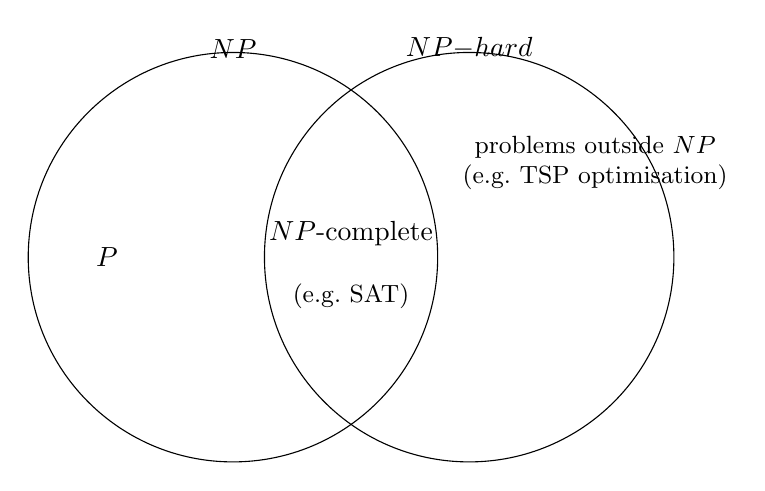
\begin{tikzpicture}[scale=1]
 \draw (0,0) circle (2.6cm) node[above,yshift=2.4cm] {$NP$};
 \draw (3,0) circle (2.6cm) node[above,yshift=2.4cm] {$NP\text{-hard}$};
 \node at (-1.6,0) {$P$};
 \node[align=center] at (1.5,0.3) {$NP$-complete};
 \node[align=center,font=\small] at (1.5,-0.5) {(e.g.\ SAT)};
 \node[align=center,font=\small] at (4.6,1.2) {problems outside $NP$\\(e.g.\ TSP optimisation)};
\end{tikzpicture}
\end{center}

\noindent The left circle is $NP$ (decision problems with polynomial-time-verifiable certificates); the right circle is $NP$-hard (everything at least as hard as every $NP$ problem, via reduction). $H$ need not lie in $NP$, so the right circle extends beyond the left one. Their intersection -- problems that are both easy to verify and at least as hard as anything in $NP$ -- is exactly $NP$-complete.

\subsection{Sums and summation}
\label{sec:6-10}
% CN 6.10 / Rosen 2.4

\begin{note}[Notation]
\[
\sum_{k=1}^n a_k = a_1+a_2+\cdots+a_n.
\]
\end{note}

\begin{example}[Double sum, swapping order]
Consider the array of values $j$ indexed by row $i=1,\dots,n$ and column $j=1,\dots,i$:
\[
\begin{array}{c|ccccc}
i \backslash j & 1 & 2 & 3 & \cdots & n \\\hline
1 & 1 & & & & \\
2 & 1 & 2 & & & \\
3 & 1 & 2 & 3 & & \\
\vdots & \vdots & \vdots & & \ddots & \\
n & 1 & 2 & 3 & \cdots & n
\end{array}
\]
Summing \emph{row by row} gives the original sum; summing \emph{column by column} gives the swapped form. Column $j$ contains the value $j$ repeated once for every row $i=j,\dots,n$, i.e.\ $n-j+1$ times:
\[
\sum_{i=1}^{n}\sum_{j=1}^{i} j
= \underbrace{(\underbrace{1+\cdots+1}_{n})}_{j=1} + \underbrace{(\underbrace{2+\cdots+2}_{n-1})}_{j=2} + \cdots + \underbrace{(n)}_{j=n,\ 1\text{ copy}}.
\]
Each column's total is $j\times(n-j+1)$ (e.g.\ column $j=2$: $2\times(n-2+1)=2(n-1)$, matching $n-1$ copies of $2$). Summing over columns instead of rows swaps the order of summation:
\[
\sum_{i=1}^{n}\sum_{j=1}^{i} j = \sum_{j=1}^{n}\sum_{i=j}^{n} j = \sum_{j=1}^n j(n-j+1).
\]
The first equality swaps summation order (the region $1\le j\le i\le n$ described either "by rows" or "by columns"); the second collapses the inner sum since $j$ is constant over $i=j,\dots,n$, contributing $n-j+1$ copies.
\end{example}

\begin{example}[Same sum, expanded directly]
Writing out the inner sum $\sum_{j=1}^i j = 1+2+\cdots+i$ for each $i$ before summing over $i$ gives the same total from a different angle:
\[
\sum_{i=1}^{n}\sum_{j=1}^{i} j = \sum_{i=1}^n(1+2+\cdots+i) = 1+(1+2)+(1+2+3)+\cdots+(1+\cdots+n).
\]
This makes the triangular shape of the summation region visible directly: the $i$-th block has length $i$, so the blocks grow row by row -- the same picture that the swapped form in the example above sums up column by column instead.
\end{example}

\begin{example}[Telescoping sum -- harder]
\[
\sum_{k=1}^n \frac{1}{k(k+1)} = \sum_{k=1}^n\left(\frac1k-\frac1{k+1}\right) = 1-\frac1{n+1},
\]
since every interior term cancels: $\left(1-\tfrac12\right)+\left(\tfrac12-\tfrac13\right)+\cdots+\left(\tfrac1n-\tfrac1{n+1}\right)$, leaving only the first and last pieces.
\end{example}

\bigskip
\begin{theorem}[Abel summation (summation by parts) -- beyond Rosen, genuinely advanced]
For sequences $(a_k),(b_k)$, let $A_n=\sum_{k=1}^n a_k$. Then
\[
\sum_{k=1}^n a_k b_k = A_n b_n - \sum_{k=1}^{n-1} A_k(b_{k+1}-b_k).
\]
\end{theorem}
\begin{proof}
Write $a_k = A_k-A_{k-1}$ (with $A_0=0$). Then
\[
\sum_{k=1}^n a_kb_k = \sum_{k=1}^n(A_k-A_{k-1})b_k = \sum_{k=1}^n A_kb_k - \sum_{k=1}^n A_{k-1}b_k.
\]
Re-index the second sum ($j=k-1$): $\sum_{j=0}^{n-1}A_jb_{j+1} = \sum_{j=1}^{n-1}A_jb_{j+1}$ (since $A_0=0$). So
\[
\sum_{k=1}^n a_kb_k = A_nb_n + \sum_{k=1}^{n-1}A_k(b_k-b_{k+1}) = A_nb_n - \sum_{k=1}^{n-1}A_k(b_{k+1}-b_k).
\]
\end{proof}

\begin{note}[The discrete analogue of integration by parts]
$A_n$ plays the role of an antiderivative of $a_k$; $b_{k+1}-b_k$ is a discrete derivative -- $\int u\,dv = uv-\int v\,du$ with sums replacing integrals. This underlies proving convergence of series like $\sum\frac{(-1)^k}{k}$ that don't converge absolutely.
\end{note}

\subsection{Finite series}
\label{sec:6-11}
% CN 6.11

\begin{note}
A \emph{finite series} is the sum of a finite sequence's terms; a \emph{partial sum} $S_n=\sum_{k=1}^n a_k$ of an infinite sequence.
\end{note}

\subsection{Finite arithmetic series}
\label{sec:6-12}
% CN 6.12

\begin{theorem}
\[
\sum_{k=1}^n (a+(k-1)d) = n\cdot\frac{2a+(n-1)d}{2}.
\]
\end{theorem}

\begin{example}[Deriving $\sum k^2$ by telescoping, before proving it -- zhangzhusheng-style construction]
Start from the identity
\[
(k+1)^3 - k^3 = 3k^2+3k+1.
\]
Sum both sides for $k=1,\dots,n$. The left side telescopes:
\[
\sum_{k=1}^n \big[(k+1)^3-k^3\big] = (n+1)^3 - 1^3,
\]
since every intermediate term cancels: $(2^3-1^3)+(3^3-2^3)+\cdots+((n{+}1)^3-n^3)$.

The right side sums termwise:
\[
\sum_{k=1}^n(3k^2+3k+1) = 3\sum_{k=1}^n k^2 + 3\sum_{k=1}^n k + n = 3\sum_{k=1}^n k^2 + 3\cdot\frac{n(n+1)}{2} + n.
\]

Equating and solving for $\sum k^2$:
\[
(n+1)^3-1 = 3\sum_{k=1}^n k^2 + \frac{3n(n+1)}{2}+n \quad\Longrightarrow\quad \sum_{k=1}^n k^2 = \frac{(n+1)^3-1-n-\frac{3n(n+1)}{2}}{3}.
\]

Simplifying the numerator (common denominator $2$, expand $(n+1)^3=n^3+3n^2+3n+1$):
\[
(n+1)^3-1-n-\tfrac{3n(n+1)}{2} = n^3+3n^2+3n-n-\tfrac{3n^2+3n}{2} = \tfrac{2n^3+6n^2+4n-3n^2-3n}{2} = \tfrac{2n^3+3n^2+n}{2} = \tfrac{n(n+1)(2n+1)}{2}.
\]

Dividing by $3$:
\[
\sum_{k=1}^n k^2 = \frac{n(n+1)(2n+1)}{6}.
\]
\end{example}

\begin{note}[Why this method matters]
Unlike the induction proof below (which needs the formula \emph{guessed} first), this telescoping method \emph{derives} the formula from scratch -- the same technique, using $(k+1)^4-k^4$, derives $\sum k^3$, and in general $(k+1)^{m+1}-k^{m+1}$ derives $\sum k^m$ for any $m$, always reducing to lower-power sums already known.
\end{note}

\subsection{Finite geometric series}
\label{sec:6-13}
% CN 6.13

\begin{theorem}
For $r\neq1$:
\[
\sum_{k=0}^n ar^k = a\cdot\frac{r^{n+1}-1}{r-1}.
\]
\end{theorem}

\bigskip
\begin{example}[Sum $\sum k\cdot2^k$ -- via differentiating a generating function, harder]
Start from $\sum_{k=0}^n x^k = \dfrac{x^{n+1}-1}{x-1}$. Differentiate both sides with respect to $x$:
\[
\sum_{k=0}^n kx^{k-1} = \frac{(n+1)x^n(x-1)-(x^{n+1}-1)}{(x-1)^2}.
\]
Multiply by $x$ and substitute $x=2$:
\[
\sum_{k=0}^n k2^k = 2\big[(n+1)2^n\cdot1-(2^{n+1}-1)\big] = (n-1)2^{n+1}+2.
\]
\end{example}

\subsection{Infinite geometric series}
\label{sec:6-14}
% CN 6.14

\begin{theorem}[Convergence condition, via \S\ref{sec:6-8}'s rigorous limit machinery]
\[
\sum_{k=0}^\infty ar^k = \frac{a}{1-r} \iff |r|<1.
\]
\end{theorem}
\begin{proof}
The partial sums $S_n = a\dfrac{1-r^{n+1}}{1-r}$. By \S\ref{sec:6-8}'s example ($r^n\to0$ for $|r|<1$, established rigorously via $\varepsilon$-$N$), $S_n \to \dfrac{a}{1-r}$. For $|r|\ge1$, $r^n$ does not $\to0$ (it diverges, or stays $\ge1$ in absolute value), so $S_n$ has no finite limit.
\end{proof}

\subsection{Harmonic numbers}
\label{sec:6-15}
% CN 6.15

\begin{definition}[Harmonic numbers]
\[
H_n = 1+\frac12+\frac13+\cdots+\frac1n.
\]
\end{definition}

\begin{theorem}[Divergence of the harmonic series]
$H_n\to\infty$ as $n\to\infty$, despite $1/n\to0$.
\end{theorem}
\begin{proof}[Classical proof, grouping by powers of $2$]
Group terms:
\[
H_{2^k} = 1 + \frac12 + \left(\frac13+\frac14\right) + \left(\frac15+\cdots+\frac18\right) + \cdots + \left(\frac{1}{2^{k-1}+1}+\cdots+\frac{1}{2^k}\right).
\]
The block from $\frac{1}{2^{j-1}+1}$ to $\frac{1}{2^j}$ has $2^{j-1}$ terms, each $\ge \dfrac{1}{2^j}$, so the block sums to $\ge 2^{j-1}\cdot\dfrac{1}{2^j}=\dfrac12$. There are $k$ such blocks (for $j=1,\dots,k$), so
\[
H_{2^k} \ge 1+\frac{k}{2}.
\]
Since $1+k/2\to\infty$, $H_{2^k}\to\infty$, and $H_n$ is increasing, so $H_n\to\infty$.
\end{proof}

\begin{note}
This is exactly the same bound proved earlier by induction (\S\ref{sec:3-11}'s harmonic-numbers theorem, $H_{2^n}\ge1+n/2$) -- here derived directly, without induction, by explicit grouping.
\end{note}

\begin{note}[Contrast: convergent vs.\ divergent zero-limit sequences]
$(1/n^2)$ and $(1/2^n)$ both $\to0$ with \emph{finite} sum (the latter by \S\ref{sec:6-14}'s geometric series). $(1/n)$ is the borderline case: it decays just slowly enough to have infinite sum -- among decaying sequences, $1/n$ marks roughly where convergence of the sum starts to fail (the $p$-series $\sum1/n^p$ converges for $p>1$, diverges for $p\le1$).
\end{note}

\begin{note}[Euler's constant]
\[
\lim_{n\to\infty}(H_n-\ln n) = \gamma = 0.5772\dots,
\]
so $H_n \approx \ln n+\gamma$ for large $n$. Whether $\gamma$ is rational is unknown -- an open problem.
\end{note}

\newpage

\section{Number Theory}
\label{sec:numbertheory}

\subsection{Multiples and divisors}
\label{sec:divisors}

\begin{definition}[Divisibility]
For $d\in\Z\setminus\{0\}$ and $n\in\Z$, we say $d$ \emph{divides} $n$, written $d\mid n$, if
\[
\exists q\in\Z\quad n=qd.
\]
Then $d$ is a \emph{divisor} (or \emph{factor}) of $n$, and $n$ is a \emph{multiple} of $d$. We write $d\nmid n$ otherwise. The set of all multiples of $d$ is
\[
d\Z=\{kd : k\in\Z\}.
\]
A divisor of $n$ is \emph{proper} if it is neither $1$ nor $n$.
\end{definition}

\begin{note}
$d\mid 0$ for every $d\ne 0$, since
\[
0=0\cdot d.
\]
Zero must often be treated as a special case.
\end{note}

\begin{theorem}[Linearity of divisibility]
\label{thm:divlinear}
For all $d,m,n,x,y\in\Z$ with $d\ne0$,
\[
d\mid m \ \wedge\ d\mid n \quad\Longrightarrow\quad d\mid (xm+yn).
\]
In particular $d\mid(m+n)$ and $d\mid(m-n)$.
\end{theorem}

\begin{proof}
Write
\[
m=q_1d, \qquad n=q_2d.
\]
Then
\[
xm+yn=(xq_1+yq_2)d,
\]
and $xq_1+yq_2\in\Z$.
\end{proof}

\begin{note}
The converse fails: $2\mid(3+5)$ but $2\nmid3$ and $2\nmid5$.
\end{note}

\begin{example}[Divisibility by a product of consecutive integers -- harder]
Prove
\[
6\mid n(n+1)(n+2)
\]
for all $n\in\Z$.

\smallskip
Among any three consecutive integers, at least one is even, so $2\mid n(n+1)(n+2)$.

\smallskip
Writing $n\equiv r\pmod 3$ with $r\in\{0,1,2\}$:
\begin{itemize}
\item if $r=0$ then $3\mid n$;
\item if $r=1$ then $3\mid(n+2)$;
\item if $r=2$ then $3\mid(n+1)$.
\end{itemize}
So $3\mid n(n+1)(n+2)$ in every case. Since $\gcd(2,3)=1$, Theorem~\ref{thm:coprimedivides} gives $6\mid n(n+1)(n+2)$.
\end{example}

\begin{example}[Divisibility tests, beyond CN -- Rosen \S4.1]
Let $n$ have decimal digits $a_k\cdots a_1a_0$, i.e.
\[
n=\sum_{i=0}^{k}a_i10^i.
\]
Since $10^i\equiv0\pmod{2^j}$ for $i\ge j$, the residue $n\bmod 2^j$ depends only on the last $j$ digits:
\[
2^j\mid n \iff 2^j \mid \sum_{i=0}^{j-1}a_i10^i.
\]
This is why $4\mid n$ is decided by the last two digits and $8\mid n$ by the last three. The same argument with $5^j$ gives the tests for $5,25,125$.

\smallskip
In general, divisibility by $d$ is decidable from a bounded number of trailing decimal digits precisely when $d\mid 10^j$ for some $j$, i.e.\ when $d=2^a5^b$.
\end{example}

\subsection{Prime numbers}
\label{sec:primes}

\begin{definition}[Prime, composite]
An integer $p>1$ is \emph{prime} if it has no proper divisors. An integer $n>1$ that is not prime is \emph{composite}.
\end{definition}

\begin{theorem}[Existence of prime factorisation]
\label{thm:primefactexists}
Every integer $n\ge2$ is a product of primes.
\end{theorem}

\begin{proof}
By strong induction on $n$.

\medskip
\noindent\textbf{Basis.} $n=2$ is prime, hence a product of one prime.

\medskip
\noindent\textbf{Inductive step.} Let $n\ge2$ and assume every $k$ with $2\le k\le n$ is a product of primes. Consider $n+1$.

\begin{itemize}
\item If $n+1$ is prime, it is a product of one prime.
\item If $n+1$ is composite, it has a divisor $a$ with $1<a<n+1$. Set
\[
b=\frac{n+1}{a}\in\Z.
\]
Then $1<b<n+1$ as well: if $b=1$ then $a=n+1$, and if $b=n+1$ then $a=1$, both contradicting the choice of $a$. Since $a,b\le n$, the inductive hypothesis applies to each, so both are products of primes, hence so is $n+1=ab$.
\end{itemize}

\medskip
\noindent By strong induction the claim holds for all $n\ge2$.
\end{proof}

\begin{theorem}[Infinitude of primes, Euclid -- Rosen \S4.3]
\label{thm:infprimes}
There are infinitely many primes.
\end{theorem}

\begin{proof}
Suppose the primes are exactly $p_1,\dots,p_k$. Let
\[
N=p_1p_2\cdots p_k+1.
\]
By Theorem~\ref{thm:primefactexists}, $N$ has a prime divisor $p_i$ for some $i$. But $p_i\mid p_1\cdots p_k$, so by Theorem~\ref{thm:divlinear}
\[
p_i\mid (N-p_1\cdots p_k) = 1,
\]
which is impossible for a prime. Hence no finite list contains all primes.
\end{proof}

\begin{theorem}[Trial division bound -- Rosen \S4.3]
\label{thm:sqrtbound}
If $n>1$ is composite, then $n$ has a prime divisor $p\le\sqrt n$.
\end{theorem}

\begin{proof}
Write $n=ab$ with $1<a\le b<n$. Then
\[
a^2\le ab=n, \qquad\text{so}\qquad a\le\sqrt n.
\]
By Theorem~\ref{thm:primefactexists}, $a$ has a prime divisor $p\le a\le\sqrt n$, and $p\mid a\mid n$.
\end{proof}

\begin{note}[Extra: density of primes]
The Prime Number Theorem states that $\pi(x)$, the number of primes $\le x$, satisfies
\[
\pi(x)\sim\frac{x}{\ln x}.
\]
So primes thin out, but only logarithmically: a random integer near $x$ is prime with probability roughly $1/\ln x$. This is what makes random search for large primes (as needed in \S\ref{sec:diffiehellman}) practical.
\end{note}

\begin{example}[A composite family -- harder, Sophie Germain identity]
Show that $n^4+4$ is composite for every integer $n>1$.

\smallskip
Complete the square twice:
\[
n^4+4 = (n^4+4n^2+4)-4n^2 = (n^2+2)^2-(2n)^2 = (n^2-2n+2)(n^2+2n+2).
\]
For $n>1$ we have
\[
n^2-2n+2=(n-1)^2+1\ge2, \qquad n^2+2n+2>n^2-2n+2,
\]
so both factors are proper. Hence $n^4+4$ is composite.
\end{example}

\subsection{Remainders and the mod operation}
\label{sec:mod}

\begin{theorem}[Division algorithm -- Rosen \S4.1, more rigorous than CN's statement: uniqueness included]
\label{thm:division}
For all $n\in\Z$ and $d\in\N$ there exist \emph{unique} $q,r\in\Z$ with
\[
n=qd+r, \qquad 0\le r\le d-1.
\]
\end{theorem}

\begin{proof}
\textbf{Existence.} Let
\[
S=\{n-kd : k\in\Z,\ n-kd\ge0\}.
\]
$S$ is nonempty (take $k=-|n|$, giving $n+|n|d\ge0$), so by well-ordering it has a least element $r=n-qd\ge0$. If $r\ge d$ then
\[
r-d=n-(q+1)d\ge0
\]
lies in $S$ and is smaller, a contradiction. So $0\le r\le d-1$.

\medskip
\noindent\textbf{Uniqueness.} Suppose $n=q_1d+r_1=q_2d+r_2$ with $0\le r_1,r_2\le d-1$. Then
\[
r_1-r_2=(q_2-q_1)d,
\]
so $d\mid(r_1-r_2)$. But $|r_1-r_2|\le d-1<d$, forcing $r_1=r_2$, and then $q_1=q_2$ since $d\ne0$.
\end{proof}

\begin{definition}[The mod operation]
The unique $r$ of Theorem~\ref{thm:division} is written $n\bmod d$, and $q=\lfloor n/d\rfloor$. Thus
\[
\frac nd = \left\lfloor\frac nd\right\rfloor + \frac{n\bmod d}{d}, \qquad \frac{n\bmod d}{d}\in[0,1).
\]
\end{definition}

\begin{note}
The divisor $d$ is always taken positive; $n$ may be negative. For example,
\[
-6\bmod5=4,
\]
since the largest multiple of $5$ that is $\le-6$ is $-10$ (so $q=-2$) and $-10+4=-6$. Programming languages' \texttt{\%} operator need not agree with $\bmod$ on negative arguments.
\end{note}

\subsection{Parity}
\label{sec:parity}

\begin{definition}[Parity]
The \emph{parity} of $x\in\Z$ is $x\bmod2$; $x$ is \emph{even} if this is $0$ and \emph{odd} if it is $1$.
\end{definition}

\begin{note}[Parity as Boolean algebra]
Writing parities as $0,1$, the addition and multiplication tables mod $2$ are

\begin{center}
$
\begin{array}{c|cc}
+ & 0 & 1\\\hline
0 & 0 & 1\\
1 & 1 & 0
\end{array}
\qquad\qquad
\begin{array}{c|cc}
\times & 0 & 1\\\hline
0 & 0 & 0\\
1 & 0 & 1
\end{array}
$
\end{center}

These are exactly the truth tables of $\oplus$ (exclusive-or) and $\wedge$ (conjunction) with $0=$ False, $1=$ True. So $\Z_2$ with $+,\times$ \emph{is} propositional logic with $\oplus,\wedge$, up to renaming -- an \emph{isomorphism}. This identification underlies the use of logic gates to perform arithmetic.
\end{note}

\begin{example}[Parity argument -- harder]
Prove $\sqrt2\notin\Q$.

\smallskip
Suppose
\[
\sqrt2=\frac ab, \qquad a,b\in\N,\ \gcd(a,b)=1.
\]
Then $a^2=2b^2$, so $a^2$ is even. Since the square of an odd number is odd, $a$ must be even; write $a=2c$. Then
\[
4c^2=2b^2 \quad\Longrightarrow\quad b^2=2c^2,
\]
and by the same argument $b$ is even. Then $2\mid\gcd(a,b)=1$, a contradiction.
\end{example}

\subsection{The greatest common divisor}
\label{sec:gcd}

\begin{definition}[gcd, lcm]
For $a,b\in\Z$ not both $0$, $\gcd(a,b)$ is the greatest $d$ with $d\mid a$ and $d\mid b$. For $a,b\in\N$, $\lcmop(a,b)$ is the least positive common multiple.
\end{definition}

\begin{note}
$\gcd(a,b)$ is well defined: the set of common divisors is nonempty (it contains $1$) and bounded above (since $d\mid n\ne0\Rightarrow d\le|n|$), and every bounded nonempty set of integers has a greatest element. If $a=b=0$ every integer is a common divisor, so $\gcd(0,0)$ is undefined.
\end{note}

\begin{theorem}[Subtraction invariance]
\label{thm:gcdsub}
For $a,b\in\Z$ not both $0$,
\[
\gcd(a,b)=\gcd(b,a-b).
\]
\end{theorem}

\begin{proof}
Let
\[
\mathrm{CD}(x,y)=\{d : d\mid x \wedge d\mid y\}.
\]
We show $\mathrm{CD}(a,b)=\mathrm{CD}(b,a-b)$.

\medskip
\noindent$(\subseteq)$ If $d\mid a$ and $d\mid b$ then $d\mid(a-b)$ by Theorem~\ref{thm:divlinear}, so $d\in\mathrm{CD}(b,a-b)$.

\medskip
\noindent$(\supseteq)$ If $d\mid b$ and $d\mid(a-b)$ then
\[
d\mid\bigl((a-b)+b\bigr)=a,
\]
so $d\in\mathrm{CD}(a,b)$.

\medskip
\noindent Both sets are nonempty and bounded above, hence each has a greatest element; equal sets have equal greatest elements.
\end{proof}

\begin{theorem}[gcd--lcm identity -- Rosen \S4.3, beyond CN]
\label{thm:gcdlcm}
For $a,b\in\N$,
\[
\gcd(a,b)\cdot\lcmop(a,b)=ab.
\]
\end{theorem}

\begin{proof}
Write $a=\prod_i p_i^{e_i}$ and $b=\prod_i p_i^{f_i}$ over a common list of primes (Theorem~\ref{thm:fta}). Then
\[
\gcd(a,b)=\prod_i p_i^{\min(e_i,f_i)}, \qquad \lcmop(a,b)=\prod_i p_i^{\max(e_i,f_i)},
\]
and $\min(e_i,f_i)+\max(e_i,f_i)=e_i+f_i$ for each $i$.
\end{proof}

\subsection{The Euclidean algorithm}
\label{sec:euclid}

\begin{definition}[Euclidean Algorithm (EA)]
\begin{enumerate}
\item Input $a,b\in\N$; if $a<b$, swap so that $a\ge b$.
\item If $b\mid a$, output $b$.
\item Let
\[
q:=\left\lfloor\frac ab\right\rfloor;
\]
output
\[
\gcd(b,\,a-qb)=\gcd(b,\,a\bmod b).
\]
\end{enumerate}
\end{definition}

\begin{note}
Repeated subtraction (Theorem~\ref{thm:gcdsub}) is replaced by a single remainder computation, since subtracting $b$ from $a$ until the result drops below $b$ is exactly division with remainder.
\end{note}

\begin{theorem}[Lamé's theorem -- Rosen \S4.3, beyond CN]
\label{thm:lame}
The number of divisions used by the Euclidean algorithm on $a>b\ge1$ is at most $5$ times the number of decimal digits of $b$.
\end{theorem}

\begin{proof}[Proof sketch]
Let the algorithm perform $n$ divisions on $(r_0,r_1)=(a,b)$, producing
\[
r_0>r_1>\cdots>r_n>r_{n+1}=0.
\]
Each step gives $r_{k-1}=q_kr_k+r_{k+1}$ with $q_k\ge1$, so $r_{k-1}\ge r_k+r_{k+1}$. Comparing with the Fibonacci recurrence and $r_n\ge1=f_2$ gives $b=r_1\ge f_{n+1}$ by induction. By Binet's formula (Theorem~\ref{thm:binet}),
\[
f_{n+1}>\varphi^{n-1},
\]
so $n-1<\log_\varphi b$. Since $\log_{10}\varphi>1/5$, we get $n<5\log_{10}b+1$, i.e.\ $n$ is at most $5$ times the digit count of $b$.
\end{proof}

\begin{example}[Worst case of the EA -- harder]
Consecutive Fibonacci numbers are the worst case: $\gcd(f_{n+1},f_n)$ takes exactly $n-1$ divisions. For example, for $(55,34)$:
\[
55=1\cdot34+21, \qquad 34=1\cdot21+13, \qquad 21=1\cdot13+8, \qquad 13=1\cdot8+5,
\]
\[
8=1\cdot5+3, \qquad 5=1\cdot3+2, \qquad 3=1\cdot2+1, \qquad 2=2\cdot1+0,
\]
so $\gcd(55,34)=1$. Every quotient is $1$ (except the last), which is the slowest possible descent -- each remainder is the previous Fibonacci number. Consecutive Fibonacci numbers are therefore always coprime.
\end{example}

\subsection{The gcd and integer linear combinations}
\label{sec:bezout}

\begin{definition}[Integer linear combinations]
For $m,n\in\Z$,
\[
m\Z+n\Z=\{xm+yn : x,y\in\Z\}.
\]
\end{definition}

\begin{theorem}
\label{thm:deltaZ}
Let $m,n\in\N$ and let $\Delta$ be the least positive element of $m\Z+n\Z$. Then
\[
m\Z+n\Z=\Delta\Z.
\]
\end{theorem}

\begin{proof}
\noindent$(\supseteq)$ Write $\Delta=x_0m+y_0n$. For $k\in\Z$,
\[
k\Delta=(kx_0)m+(ky_0)n\in m\Z+n\Z.
\]

\medskip
\noindent$(\subseteq)$ Let $z=xm+yn$ and write $z=q\Delta+r$ with $0\le r<\Delta$ (Theorem~\ref{thm:division}). Since $q\Delta\in m\Z+n\Z$ and $m\Z+n\Z$ is closed under subtraction,
\[
r=z-q\Delta\in m\Z+n\Z.
\]
If $r>0$ this contradicts minimality of $\Delta$. So $r=0$ and $\Delta\mid z$.
\end{proof}

\begin{theorem}[Bézout]
\label{thm:bezout}
For $m,n\in\N$,
\[
\gcd(m,n)=\min\{xm+yn : x,y\in\Z,\ xm+yn>0\}.
\]
Equivalently, there exist $x,y\in\Z$ with
\[
\gcd(m,n)=xm+yn.
\]
\end{theorem}

\begin{proof}
With $\Delta$ as in Theorem~\ref{thm:deltaZ}, $\Delta$ divides every element of $m\Z+n\Z$, in particular $m$ and $n$, so $\Delta$ is a common divisor. Conversely any common divisor $d$ of $m,n$ divides $xm+yn$ for all $x,y$ (Theorem~\ref{thm:divlinear}), in particular $d\mid\Delta$, so $d\le\Delta$. Hence $\Delta=\gcd(m,n)$.
\end{proof}

\begin{note}
Bézout coefficients are never unique. Since $nm-mn=0$, adding $k\cdot(n,-m)$ to any solution $(x,y)$ gives another:
\[
(x+kn)m+(y-km)n = xm+yn.
\]
So each element of $m\Z+n\Z$ arises in infinitely many ways.
\end{note}

\subsection{The extended Euclidean algorithm}
\label{sec:eea}

\begin{definition}[Extended Euclidean Algorithm (EEA)]
\begin{enumerate}
\item Input $m,n\in\N$; if $m<n$, swap so that $m\ge n$.
\item Initialise
\[
(a,x,y):=(m,1,0), \qquad (b,z,w):=(n,0,1).
\]
\item If $b=0$, output $(a,x,y)$.
\item Let
\[
q:=\left\lfloor\frac ab\right\rfloor.
\]
Update
\[
(a,x,y)_{\text{new}}:=(b,z,w), \qquad (b,z,w)_{\text{new}}:=(a,x,y)-q\cdot(b,z,w),
\]
using vector subtraction on the old values. Return to step 3.
\end{enumerate}
\end{definition}

\begin{theorem}[Correctness of the EEA]
\label{thm:eea}
At every stage the triples satisfy $a=xm+yn$ and $b=zm+wn$. On termination $a=\gcd(m,n)$, so the final $a$-triple gives Bézout coefficients.
\end{theorem}

\begin{proof}
The invariant holds initially:
\[
m=1\cdot m+0\cdot n, \qquad n=0\cdot m+1\cdot n.
\]
If it holds before an update, then the new $b$-triple satisfies
\[
a-qb = (x-qz)m+(y-qw)n,
\]
which is the required form, and the new $a$-triple is the old $b$-triple. The first components evolve exactly as in the EA, so termination gives $a=\gcd(m,n)$.
\end{proof}

\begin{example}[EEA with a nontrivial gcd -- harder]
Compute $\gcd(1180,482)$ and express it as an integer linear combination. Each row $(t,x,y)$ satisfies $t=1180x+482y$:
\[
\begin{array}{rrrl}
1180 & 1 & 0 & \\
482 & 0 & 1 & \\
216 & 1 & -2 & (\lfloor1180/482\rfloor=2)\\
50 & -2 & 5 & (\lfloor482/216\rfloor=2)\\
16 & 9 & -22 & (\lfloor216/50\rfloor=4)\\
2 & -29 & 71 & (\lfloor50/16\rfloor=3)\\
0 & 241 & -590 & (\lfloor16/2\rfloor=8)
\end{array}
\]
So $\gcd(1180,482)=2$ and
\[
2 = -29\cdot1180 + 71\cdot482.
\]

\smallskip
\noindent\textbf{Check.} $-29\cdot1180=-34220$, $71\cdot482=34222$, difference $2$. The final row checks out too:
\[
241\cdot1180=284380=590\cdot482.
\]
Note the zig-zag of signs down the last two columns -- a useful error check.
\end{example}

\subsection{Coprimality}
\label{sec:coprime}

\begin{definition}[Coprime]
$a,b\in\Z$ are \emph{coprime} (\emph{relatively prime}) if $\gcd(a,b)=1$.
\end{definition}

\begin{note}
Coprimality is not primality: $21$ and $25$ are coprime, neither is prime. Coprimality is easy to test (run the EA); primality testing is a genuinely different and harder problem.
\end{note}

\begin{theorem}[Bézout characterisation of coprimality]
\label{thm:coprimebezout}
$m,n\in\Z$ are coprime if and only if there exist $x,y\in\Z$ with
\[
xm+yn=1.
\]
\end{theorem}

\begin{proof}
By Theorem~\ref{thm:bezout}, $\gcd(m,n)$ is the least positive element of $m\Z+n\Z$. Since no positive integer is smaller than $1$, this least element equals $1$ iff $1\in m\Z+n\Z$.
\end{proof}

\begin{theorem}[Euclid's lemma]
\label{thm:euclidlemma}
Let $p$ be prime and $a,b\in\Z$. Then
\[
p\mid ab \quad\Longrightarrow\quad p\mid a \ \vee\ p\mid b.
\]
\end{theorem}

\begin{proof}
Assume $p\mid ab$ and $p\nmid a$. Since $p$ is prime and $p\nmid a$, $\gcd(p,a)=1$, so by Theorem~\ref{thm:coprimebezout} there are $x,y\in\Z$ with
\[
xp+ya=1.
\]
Multiply by $b$:
\[
xpb+yab=b.
\]
The first summand is a multiple of $p$; the second is a multiple of $ab$, hence of $p$ by assumption. So $p\mid b$.
\end{proof}

\begin{theorem}[Coprime divisor rule -- Rosen \S4.3]
\label{thm:coprimedivides}
If $a\mid n$, $b\mid n$ and $\gcd(a,b)=1$, then $ab\mid n$.
\end{theorem}

\begin{proof}
Write $xa+yb=1$ (Theorem~\ref{thm:coprimebezout}) and $n=a\alpha=b\beta$. Then
\[
n = n(xa+yb) = xan+ybn = xa(b\beta)+yb(a\alpha) = ab(x\beta+y\alpha).
\]
\end{proof}

\begin{theorem}[Fundamental Theorem of Arithmetic]
\label{thm:fta}
Every positive integer has a factorisation into primes that is unique up to order.
\end{theorem}

\begin{proof}
Existence is Theorem~\ref{thm:primefactexists}. For uniqueness, suppose some integer has two distinct prime factorisations and let $n$ be the smallest such. Write, over the primes $p_1,\dots,p_k$ appearing in either factorisation,
\[
n=p_1^{e_1}\cdots p_k^{e_k}=p_1^{f_1}\cdots p_k^{f_k},
\]
with $e_i,f_i\ge0$ not both zero for each $i$, and $e_i\ne f_i$ for some $i$.

\medskip
\noindent Suppose some $p_j$ has $e_j>0$ and $f_j>0$. Put
\[
g_j=\min(e_j,f_j)>0
\]
and divide both factorisations by $p_j^{g_j}$. Some prime still has unequal exponents in the two results (if $e_j\ne f_j$ then $p_j$ does; otherwise $p_i$ does), so $n/p_j^{g_j}<n$ has two distinct prime factorisations, contradicting minimality of $n$.

\medskip
\noindent Hence the two factorisations use disjoint sets of primes. Let $p$ occur in the first. Then $p\mid n$, and $n$ is a product of primes $q_1,\dots,q_l$ none equal to $p$. Repeated application of Theorem~\ref{thm:euclidlemma} gives $p\mid q_t$ for some $t$, so $p=q_t$ -- a contradiction.
\end{proof}

\subsection{Modular arithmetic}
\label{sec:modarith}

\begin{definition}[Congruence]
For $n\in\N$ and $a,b\in\Z$, $a$ and $b$ are \emph{congruent modulo $n$}, written $a\equiv b\pmod n$, if $n\mid(a-b)$.
\end{definition}

\begin{theorem}
\label{thm:congremainder}
\[
a\equiv b\pmod n \quad\Longleftrightarrow\quad a\bmod n=b\bmod n.
\]
\end{theorem}

\begin{proof}
Write
\[
a=q_an+r_a, \qquad b=q_bn+r_b, \qquad 0\le r_a,r_b\le n-1.
\]
Then
\[
a-b=(q_a-q_b)n+(r_a-r_b),
\]
so $n\mid(a-b)$ iff $n\mid(r_a-r_b)$. But $|r_a-r_b|\le n-1<n$, so this holds iff $r_a=r_b$.
\end{proof}

\begin{theorem}
\label{thm:congequiv}
For every $n\in\N$, congruence modulo $n$ is an equivalence relation on $\Z$.
\end{theorem}

\begin{proof}
\textbf{Reflexive:} $a-a=0=0\cdot n$.

\smallskip
\noindent\textbf{Symmetric:} if $a-b=kn$ then $b-a=(-k)n$.

\smallskip
\noindent\textbf{Transitive:} if $a-b=kn$ and $b-c=ln$ then $a-c=(k+l)n$.
\end{proof}

\begin{definition}[Residue classes and $\Z_n$]
The equivalence classes of congruence mod $n$ are the \emph{residue classes}
\[
[a]=a+n\Z=\{a+kn : k\in\Z\},
\]
and there are exactly $n$ of them: $[0],[1],\dots,[n-1]$. We write $\Z_n=\{0,1,\dots,n-1\}$, equipped with $+,-,\times$ followed by reduction mod $n$.
\end{definition}

\begin{theorem}[Congruences respect arithmetic -- Rosen \S4.1, stated more generally than CN]
\label{thm:congarith}
If $a\equiv b\pmod n$ and $c\equiv d\pmod n$, then
\[
a+c\equiv b+d\pmod n, \qquad a-c\equiv b-d\pmod n, \qquad ac\equiv bd\pmod n.
\]
\end{theorem}

\begin{proof}
Write $a-b=kn$, $c-d=ln$. Then
\[
(a+c)-(b+d)=(k+l)n, \qquad (a-c)-(b-d)=(k-l)n.
\]
For the product,
\[
ac-bd = ac-bc+bc-bd = c(a-b)+b(c-d) = (ck+bl)n. \qedhere
\]
\end{proof}

\begin{note}
Theorem~\ref{thm:congarith} justifies reducing mod $n$ \emph{at every step} of a computation involving only $+,-,\times$, rather than only at the end. Division and exponentiation need separate treatment (\S\ref{sec:modinv}, \S\ref{sec:modexp}).
\end{note}

\begin{example}[Casting out nines -- harder]
Since $10\equiv1\pmod9$, we have $10^i\equiv1\pmod9$ for all $i$, so for $n=\sum a_i10^i$,
\[
n\equiv\sum_i a_i = \mathrm{ds}(n) \pmod 9,
\]
where $\mathrm{ds}$ is the digital sum. Hence a claimed product can be checked cheaply: the alleged identity $84\times32=2678$ fails because
\[
(84\times32)\bmod9=(3\times5)\bmod9=15\bmod9=6, \qquad 2678\bmod9=5.
\]
The check is one-sided: it detects some errors, never certifies correctness -- it is blind to any error that is a multiple of $9$, e.g.\ transposed digits. The same argument with $10\equiv-1\pmod{11}$ gives $n\equiv\mathrm{ads}(n)\pmod{11}$ for the alternating digital sum.
\end{example}

\begin{example}[Large modular power without Euler -- harder]
Find the last two decimal digits of $7^{1000}$, i.e.\ $7^{1000}\bmod100$.

\smallskip
Note
\[
7^2=49, \qquad 7^4=49^2=2401\equiv1\pmod{100}.
\]
So the powers of $7$ cycle with period $4$ mod $100$, and $1000=4\cdot250$:
\[
7^{1000}=(7^4)^{250}\equiv1^{250}=1 \pmod{100}.
\]
The last two digits are $01$.
\end{example}

\subsection{Modular inverses}
\label{sec:modinv}

\begin{definition}[Modular inverse, $\Z_n^*$]
$x^{-1}\in\Z_n$ is a \emph{multiplicative inverse} of $x\in\Z_n$ if $xx^{-1}\equiv1\pmod n$. We write $\Z_n^*$ for the set of elements of $\Z_n$ possessing an inverse.
\end{definition}

\begin{theorem}[Existence of inverses]
\label{thm:inverse}
$x\in\Z_n$ has an inverse in $\Z_n$ if and only if $\gcd(x,n)=1$.
\end{theorem}

\begin{proof}
\noindent$(\Rightarrow)$ If $xx^{-1}\equiv1\pmod n$ then $xx^{-1}+kn=1$ for some $k\in\Z$, so $x$ and $n$ are coprime by Theorem~\ref{thm:coprimebezout}.

\medskip
\noindent$(\Leftarrow)$ If $\gcd(x,n)=1$, Theorem~\ref{thm:coprimebezout} gives $y,z\in\Z$ with
\[
yx+zn=1.
\]
Let $y'=y\bmod n$, so $y=ln+y'$. Then
\[
y'x+(lx+z)n=1,
\]
so $y'x\equiv1\pmod n$ with $y'\in\Z_n$.
\end{proof}

\begin{note}
The proof is constructive: run the EEA on $(x,n)$ to obtain $y,z$ with $yx+zn=1$; then $x^{-1}=y\bmod n$. This is the principal practical use of the EEA.
\end{note}

\begin{example}[Inverse computation -- harder]
Find $17^{-1}$ in $\Z_{101}$. Rows $(t,x,y)$ satisfy $t=101x+17y$:
\[
\begin{array}{rrrl}
101 & 1 & 0 &\\
17 & 0 & 1 &\\
16 & 1 & -5 & (\lfloor101/17\rfloor=5)\\
1 & -1 & 6 & (\lfloor17/16\rfloor=1)\\
0 & 17 & -101 & (\lfloor16/1\rfloor=16)
\end{array}
\]
So
\[
1=-1\cdot101+6\cdot17,
\]
giving $17^{-1}\equiv6\pmod{101}$. Check: $6\cdot17=102\equiv1\pmod{101}$.
\end{example}

\begin{theorem}[Linear congruences -- Rosen \S4.4, beyond CN]
\label{thm:lincong}
Let $d=\gcd(a,n)$. The congruence $ax\equiv b\pmod n$ has a solution if and only if $d\mid b$, in which case it has exactly $d$ solutions in $\Z_n$.
\end{theorem}

\begin{proof}
$ax\equiv b\pmod n$ has a solution iff $b\in a\Z+n\Z$, which by Theorem~\ref{thm:deltaZ} equals $d\Z$; so solvability is exactly $d\mid b$. If $d\mid b$, divide through:
\[
\frac ad\,x\equiv\frac bd \pmod{n/d},
\]
where $\gcd(a/d,n/d)=1$, so by Theorem~\ref{thm:inverse} there is a unique solution $x_0$ mod $n/d$. Its lifts $x_0,x_0+n/d,\dots,x_0+(d-1)n/d$ are the $d$ solutions in $\Z_n$.
\end{proof}

\begin{theorem}[Chinese Remainder Theorem -- Rosen \S4.4, beyond CN]
\label{thm:crt}
Let $n_1,\dots,n_k$ be pairwise coprime and $N=n_1\cdots n_k$. Then the system
\[
x\equiv a_i \pmod{n_i}, \qquad i=1,\dots,k,
\]
has a unique solution modulo $N$.
\end{theorem}

\begin{proof}
Let $N_i=N/n_i$. Since the moduli are pairwise coprime, $\gcd(N_i,n_i)=1$, so by Theorem~\ref{thm:inverse} there is $M_i$ with $N_iM_i\equiv1\pmod{n_i}$. Set
\[
x=\sum_{i=1}^{k}a_iN_iM_i.
\]
For each $j$, every term with $i\ne j$ has $n_j\mid N_i$, so
\[
x\equiv a_jN_jM_j\equiv a_j\pmod{n_j}.
\]
For uniqueness, if $x,x'$ both solve the system then $n_i\mid(x-x')$ for all $i$, and pairwise coprimality gives $N\mid(x-x')$ by repeated use of Theorem~\ref{thm:coprimedivides}.
\end{proof}

\begin{example}[CRT -- harder]
Solve
\[
x\equiv2\pmod3, \qquad x\equiv3\pmod5, \qquad x\equiv2\pmod7.
\]

\smallskip
Here $N=105$, and $N_1=35,\ N_2=21,\ N_3=15$. Inverses:
\[
35\equiv2\pmod3,\ 2^{-1}\equiv2\pmod3; \qquad 21\equiv1\pmod5,\ 1^{-1}\equiv1; \qquad 15\equiv1\pmod7,\ 1^{-1}\equiv1.
\]
So
\[
x=2\cdot35\cdot2+3\cdot21\cdot1+2\cdot15\cdot1=140+63+30=233\equiv23\pmod{105}.
\]
Check:
\[
23=3\cdot7+2, \qquad 23=5\cdot4+3, \qquad 23=7\cdot3+2. \checkmark
\]
\end{example}

\subsection{The Euler totient function}
\label{sec:totient}

\begin{definition}[Euler totient function]
For $n\in\N$,
\[
\varphi(n)=\bigl|\{x : 0<x<n,\ \gcd(x,n)=1\}\bigr| = |\Z_n^*|,
\]
the second equality by Theorem~\ref{thm:inverse}.
\end{definition}

\begin{theorem}[Totient of a prime power]
\label{thm:totientpp}
For $p$ prime and $m\in\N$,
\[
\varphi(p^m)=p^{m-1}(p-1).
\]
In particular $\varphi(p)=p-1$.
\end{theorem}

\begin{proof}
An integer $x$ with $0<x<p^m$ fails to be coprime to $p^m$ exactly when $p\mid x$. The multiples of $p$ below $p^m$ are $p,2p,\dots,(p^{m-1}-1)p$, of which there are $p^{m-1}-1$. Hence
\[
\varphi(p^m)=(p^m-1)-(p^{m-1}-1)=p^m-p^{m-1}=p^{m-1}(p-1). \qedhere
\]
\end{proof}

\begin{theorem}[Multiplicativity]
\label{thm:totientmult}
If $\gcd(a,b)=1$ then
\[
\varphi(ab)=\varphi(a)\varphi(b).
\]
\end{theorem}

\begin{note}[Extra: why multiplicativity holds]
The Chinese Remainder Theorem (Theorem~\ref{thm:crt}) supplies a bijection
\[
\Z_{ab}\to\Z_a\times\Z_b, \qquad x\mapsto(x\bmod a,\,x\bmod b).
\]
Under it, $x$ is coprime to $ab$ iff $x\bmod a$ is coprime to $a$ and $x\bmod b$ is coprime to $b$, so the bijection restricts to $\Z_{ab}^*\to\Z_a^*\times\Z_b^*$, giving $\varphi(ab)=\varphi(a)\varphi(b)$.
\end{note}

\begin{theorem}[General formula]
\label{thm:totientformula}
If $n=p_1^{m_1}\cdots p_k^{m_k}$ with distinct primes $p_i$, then
\[
\varphi(n)=\prod_{i=1}^{k}p_i^{m_i-1}(p_i-1) = n\prod_{i=1}^{k}\left(1-\frac1{p_i}\right).
\]
In particular, for distinct primes $p,q$:
\[
\varphi(pq)=(p-1)(q-1).
\]
\end{theorem}

\begin{proof}
Distinct prime powers are coprime, so Theorem~\ref{thm:totientmult} applies repeatedly, and each factor is evaluated by Theorem~\ref{thm:totientpp}. The second form follows from
\[
p_i^{m_i-1}(p_i-1)=p_i^{m_i}\left(1-\frac1{p_i}\right). \qedhere
\]
\end{proof}

\begin{note}
Computing $\varphi(n)$ by this formula requires the prime factorisation of $n$. No method is known for computing $\varphi(n)$ from scratch that is essentially easier than factorising $n$ -- a fact the RSA cryptosystem depends on.
\end{note}

\subsection{Fast exponentiation}
\label{sec:fastexp}

\begin{definition}[Binary (square-and-multiply) exponentiation]
Write $m=\sum_{i}b_i2^i$ in binary. Then
\[
a^m=\prod_{i \,:\, b_i=1}a^{2^i},
\]
where the values $a^{2^i}$ are obtained by repeated squaring:
\[
a^{2^{i+1}}=\left(a^{2^i}\right)^2.
\]
\end{definition}

\begin{theorem}[Cost]
\label{thm:fastexpcost}
Binary exponentiation computes $a^m$ using at most $2\lfloor\log_2 m\rfloor$ multiplications.
\end{theorem}

\begin{proof}
There are $\lfloor\log_2m\rfloor$ squarings to produce $a^2,a^4,\dots,a^{2^{\lfloor\log_2m\rfloor}}$, and at most $\lfloor\log_2m\rfloor$ further multiplications to combine those $a^{2^i}$ with $b_i=1$.
\end{proof}

\begin{example}[Square-and-multiply -- harder]
Compute $3^{36}$. Since $36=100100_2=2^5+2^2$,
\[
3^{36}=3^{2^5}\cdot3^{2^2}=\Bigl(\bigl((((3^2)^2)^2)^2\bigr)^2\Bigr)\cdot(3^2)^2.
\]
The squarings give
\[
9,\ 81,\ 6561,\ 43046721,\ 1853020188851841,
\]
and one final multiplication by $81$ yields $3^{36}$. Six multiplications, versus $35$ for the naive method.
\end{example}

\subsection{Modular exponentiation}
\label{sec:modexp}

\begin{note}
Modular exponentiation is exponentiation in $\Z_n$. Two independent savings apply: reduce each intermediate product mod $n$ (Theorem~\ref{thm:congarith}), and reduce the \emph{exponent} mod $\varphi(n)$ (Theorem~\ref{thm:euler} below).
\end{note}

\begin{theorem}[Euler]
\label{thm:euler}
If $\gcd(x,n)=1$, then
\[
x^{\varphi(n)}\equiv1\pmod n.
\]
\end{theorem}

\begin{proof}
Let $\Z_n^*=\{y_1,\dots,y_{\varphi(n)}\}$. Consider $xy_1,\dots,xy_{\varphi(n)}$. These are distinct mod $n$: if $xy_i\equiv xy_j$ then multiplying by $x^{-1}$ (which exists, by Theorem~\ref{thm:inverse}) gives $y_i\equiv y_j$, hence $y_i=y_j$. They also lie in $\Z_n^*$, since a product of elements coprime to $n$ is coprime to $n$. So multiplication by $x$ permutes $\Z_n^*$, and the two lists have equal products:
\[
y_1y_2\cdots y_{\varphi(n)} \equiv (xy_1)(xy_2)\cdots(xy_{\varphi(n)}) = x^{\varphi(n)}y_1y_2\cdots y_{\varphi(n)} \pmod n.
\]
The product $y_1\cdots y_{\varphi(n)}$ lies in $\Z_n^*$, hence is invertible; multiplying both sides by its inverse gives
\[
x^{\varphi(n)}\equiv1\pmod n. \qedhere
\]
\end{proof}

\begin{corollary}[Fermat's Little Theorem]
\label{thm:flt}
If $p$ is prime and $p\nmid x$, then
\[
x^{p-1}\equiv1\pmod p.
\]
\end{corollary}

\begin{proof}
Take $n=p$ in Theorem~\ref{thm:euler} and use $\varphi(p)=p-1$ (Theorem~\ref{thm:totientpp}).
\end{proof}

\begin{note}[Group-theoretic reading, beyond CN]
$\Z_n^*$ is a group under multiplication: it is closed, associative, has identity $1$, and every element is invertible (Theorem~\ref{thm:inverse}). Lagrange's theorem gives $g^{|G|}=e$ for any $g$ in a finite group $G$; Theorem~\ref{thm:euler} is exactly this for $G=\Z_n^*$, where $|G|=\varphi(n)$.
\end{note}

\begin{example}[Exponent reduction -- harder]
Compute $3^{36}\bmod25$. First
\[
\varphi(25)=\varphi(5^2)=5\cdot4=20,
\]
and $\gcd(3,25)=1$, so by Theorem~\ref{thm:euler} the exponent may be reduced mod $20$:
\[
3^{36}\equiv3^{36\bmod20}=3^{16}\pmod{25}.
\]
Now square repeatedly mod $25$:
\[
3^2=9, \qquad 3^4=81\equiv6, \qquad 3^8\equiv6^2=36\equiv11, \qquad 3^{16}\equiv11^2=121\equiv21 \pmod{25}.
\]
So $3^{36}\equiv21\pmod{25}$ -- four multiplications rather than six, and no number ever exceeds $121$.
\end{example}

\begin{note}[Extra: pseudoprimes and Carmichael numbers -- Rosen \S4.4]
The converse of Corollary~\ref{thm:flt} fails, so it gives only a \emph{probable}-primality test. A composite $n$ with $b^{n-1}\equiv1\pmod n$ is a \emph{pseudoprime to base $b$}; e.g.\ $341=11\cdot31$ is a pseudoprime to base $2$. Worse, a \emph{Carmichael number} is composite and passes for \emph{every} base coprime to it -- the smallest is $561=3\cdot11\cdot17$. There are infinitely many, so the Fermat test alone cannot certify primality; practical tests (Miller--Rabin) strengthen it.
\end{note}

\subsection{Primitive roots}
\label{sec:primroot}

\begin{definition}[Primitive root]
Let $\gcd(x,n)=1$. Then $x$ is a \emph{primitive root} of $n$ if
\[
x^k\not\equiv1\pmod n \qquad\text{for all } k<\varphi(n),
\]
so that $\varphi(n)$ is the least positive exponent with $x^{\varphi(n)}\equiv1$. Equivalently, $x,x^2,x^3,\dots$ run through all of $\Z_n^*$; we say $x$ \emph{generates} $\Z_n^*$.
\end{definition}

\begin{example}[Primitive root and a non-example]
For $n=7$, $\varphi(7)=6$ and $\Z_7^*=\{1,\dots,6\}$. Powers of $3$:
\[
\begin{array}{c|cccccc}
k & 1&2&3&4&5&6\\\hline
3^k\bmod7 & 3&2&6&4&5&1
\end{array}
\]
All six elements appear, and $1$ is first reached at $k=6=\varphi(7)$, so $3$ is a primitive root of $7$.

\smallskip
By contrast $2^1,2^2,2^3\equiv2,4,1$, reaching $1$ at $k=3<6$; so $2$ generates only $\{1,2,4\}$ and is not a primitive root.
\end{example}

\begin{theorem}[Which moduli have primitive roots]
\label{thm:primrootexists}
$n$ has a primitive root if and only if $n\in\{1,2,4\}$ or $n=p^k$ or $n=2p^k$ for an odd prime $p$ and $k\in\N$.
\end{theorem}

\begin{theorem}[How many]
\label{thm:primrootcount}
If $n$ has a primitive root, then it has exactly $\varphi(\varphi(n))$ of them.
\end{theorem}

\begin{note}[Why $\varphi(\varphi(n))$]
Let $a$ be a primitive root of $n$. Every element of $\Z_n^*$ is $a^k$ for a unique $k\in\{1,\dots,\varphi(n)\}$, and $a^k$ is itself a primitive root iff $\gcd(k,\varphi(n))=1$: if $d=\gcd(k,\varphi(n))>1$ then
\[
(a^k)^{\varphi(n)/d}=(a^{\varphi(n)})^{k/d}\equiv1 \pmod n
\]
with exponent $\varphi(n)/d<\varphi(n)$, so $a^k$ falls short. Counting admissible $k$ gives $\varphi(\varphi(n))$.

\smallskip
For $n=7$:
\[
\varphi(\varphi(7))=\varphi(6)=\varphi(2)\varphi(3)=2,
\]
and indeed the primitive roots are $3^1=3$ and $3^5\equiv5$, while $3^2\equiv2$, $3^3\equiv6$, $3^4\equiv4$ are not (their exponents $2,3,4$ each share a factor with $6$).
\end{note}

\begin{example}[No primitive root -- harder]
Show $8$ has no primitive root. Here $\varphi(8)=4$ and $\Z_8^*=\{1,3,5,7\}$. But
\[
3^2=9\equiv1, \qquad 5^2=25\equiv1, \qquad 7^2=49\equiv1 \pmod 8,
\]
so every element of $\Z_8^*$ satisfies $x^2\equiv1$, reaching $1$ at exponent $2<4=\varphi(8)$. Elements outside $\Z_8^*$ cannot help: powers of $2$ give $2,4,0,0,\dots$ and never reach $1$. So $\Z_8^*$ has no generator -- consistent with Theorem~\ref{thm:primrootexists}, since $8=2^3$ is a power of the \emph{even} prime.
\end{example}

\begin{note}
No fast algorithm is known for finding a primitive root of a given $n$.
\end{note}

\subsection{One-way functions}
\label{sec:oneway}

\begin{definition}[One-way function, informal]
A function $f$ is \emph{one-way} if it is easy to compute but hard to invert, for almost all inputs.
\end{definition}

\begin{note}
No function has been \emph{proved} one-way; doing so would resolve $P\ne NP$ (\S\ref{sec:pnp}). Several functions are believed to be one-way and are used as such.
\end{note}

\begin{note}[Application: password storage]
Rather than storing passwords $P_i$, a system stores pairs $(U_i,f(P_i))$ for a one-way $f$. A login attempt with password $P$ is accepted iff
\[
f(P)=f(P_i),
\]
which is fast, since $f$ is easy to compute. An attacker who obtains $f(P_i)$ faces the inversion problem. Strictly this is not encryption: no key is involved and no party is meant to recover $P_i$.
\end{note}

\subsection{Modular exponentiation with fixed base}
\label{sec:dlog}

\begin{definition}[Modular exponentiation with fixed base]
Fix $n\in\N$ and a base $a<n$. The map is
\[
x\longmapsto a^x\bmod n, \qquad x<\varphi(n).
\]
\end{definition}

\begin{definition}[Discrete Logarithm problem]
Fix $n\in\N$ and a primitive root $a$ of $n$. Given $y\in\Z_n^*$, find $x\le\varphi(n)$ with
\[
a^x\equiv y\pmod n.
\]
We write $x=\log_a y$.
\end{definition}

\begin{note}
The base is chosen to be a primitive root precisely because such a base gives the widest possible range of values (\S\ref{sec:primroot}), maximising the search space for an attacker. Discrete Logarithm is believed to have no fast algorithm -- empirically of comparable difficulty to integer factorisation. Since $\varphi(n)$ is maximised when $n$ is prime, the best candidate one-way function takes a large prime $p$ and a primitive root $a$ of $p$.
\end{note}

\subsection{Diffie--Hellman key agreement}
\label{sec:diffiehellman}

\begin{definition}[Diffie--Hellman scheme]
Public system-wide parameters: a large prime $p$ and a primitive root $a$ of $p$. Each user picks a private random $x\in\{1,\dots,p-1\}$ and publishes
\[
y=a^x\bmod p.
\]
For users $A,B$ with private numbers $x_A,x_B$ and public numbers $y_A,y_B$, each computes
\[
k_{AB} := y_B^{\,x_A}\bmod p, \qquad k_{BA} := y_A^{\,x_B}\bmod p.
\]
\end{definition}

\begin{theorem}[Agreement]
\label{thm:dhagree}
\[
k_{AB}=k_{BA}.
\]
\end{theorem}

\begin{proof}
In $\Z_p^*$,
\[
k_{AB}=y_B^{\,x_A}=(a^{x_B})^{x_A}=a^{x_Bx_A}=a^{x_Ax_B}=(a^{x_A})^{x_B}=y_A^{\,x_B}=k_{BA}. \qedhere
\]
\end{proof}

\begin{definition}[Diffie--Hellman problem]
Given $p$, $a$, $a^{x_A}\bmod p$ and $a^{x_B}\bmod p$, find
\[
a^{x_Ax_B}\bmod p.
\]
\end{definition}

\begin{theorem}
\label{thm:dhreduce}
Any algorithm for Discrete Logarithm yields an algorithm for the Diffie--Hellman problem, with only polynomial extra work.
\end{theorem}

\begin{proof}
Feed $p,a,a^{x_A}$ to the Discrete Log algorithm to recover $x_A$. Then compute
\[
(a^{x_B})^{x_A}=a^{x_Ax_B}\bmod p
\]
by fast modular exponentiation (\S\ref{sec:modexp}).
\end{proof}

\begin{note}[Open problem]
Whether the reduction goes the other way -- whether an efficient algorithm for the Diffie--Hellman problem yields one for Discrete Log -- is widely believed but unproven.
\end{note}

\begin{note}
Diffie--Hellman is a key \emph{agreement} scheme, not a cryptosystem: neither party can use it to send a message of their choosing. Its output $k_{AB}$ is then used as a key in a conventional secret-key cryptosystem. Its significance is that no secure channel is needed to establish the shared key, and neither party alone determines it.
\end{note}

\begin{example}[Diffie--Hellman with small numbers]
Take $p=11$, $a=2$, a primitive root of $11$. Alice picks $x_A=3$, Bob picks $x_B=6$:
\[
y_A=2^3\bmod11=8, \qquad y_B=2^6\bmod11=64\bmod11=9.
\]
They exchange $y_A,y_B$ and compute
\[
k_{AB}=9^3\bmod11=729\bmod11=3, \qquad k_{BA}=8^6\bmod11=262144\bmod11=3.
\]
Both equal
\[
a^{x_Ax_B}=2^{18}\equiv3\pmod{11},
\]
which neither could compute alone.
\end{example}

\begin{example}[RSA -- beyond CN, Rosen \S4.6]
Diffie--Hellman rests on Discrete Log; RSA rests on factorisation and on Theorem~\ref{thm:euler}.

\medskip
\noindent\textbf{Setup.} Choose distinct large primes $p,q$; set $n=pq$, so
\[
\varphi(n)=(p-1)(q-1)
\]
by Theorem~\ref{thm:totientformula}. Choose $e$ coprime to $\varphi(n)$ and compute $d=e^{-1}\bmod\varphi(n)$ by the EEA. Publish $(n,e)$; keep $d$ (and $p,q$) secret.

\medskip
\noindent\textbf{Encryption/decryption.}
\[
C=M^e\bmod n, \qquad M=C^d\bmod n.
\]

\medskip
\noindent\textbf{Why it inverts.} Since $ed\equiv1\pmod{\varphi(n)}$, write $ed=1+k\varphi(n)$. For $M$ coprime to $n$, Theorem~\ref{thm:euler} gives
\[
C^d = M^{ed} = M^{1+k\varphi(n)} = M\cdot\bigl(M^{\varphi(n)}\bigr)^k \equiv M\cdot1^k = M \pmod n.
\]
For $M$ not coprime to $n$ the same conclusion follows via the CRT applied mod $p$ and mod $q$ separately.

\medskip
\noindent\textbf{Security.} Recovering $d$ from $(n,e)$ requires $\varphi(n)$, which requires factorising $n$ -- believed hard. Note that anyone who learns $\varphi(n)$ can factor $n$: $p$ and $q$ are the roots of
\[
t^2-(n-\varphi(n)+1)t+n=0,
\]
since $p+q=n-\varphi(n)+1$ and $pq=n$.
\end{example}

\newpage
\section{Coungting \& Combinatoric}

\subsection{Counting by addition}
\label{sec:8-1}
% CN 8.1 / Rosen 6.1

\begin{theorem}[Sum rule]
If $A,B$ are disjoint finite sets, then $|A\cup B|=|A|+|B|$. More generally, for pairwise disjoint $A_1,\dots,A_m$:
\[
|A_1\cup A_2\cup\cdots\cup A_m| = |A_1|+|A_2|+\cdots+|A_m|.
\]
\end{theorem}
\begin{note}
Already established set-theoretically at \S\ref{sec:1-12}. Combinatorially: choosing one item from $m$ pairwise disjoint option-sets has $\sum_i|A_i|$ total possibilities.
\end{note}

\begin{example}
Two disjoint lists, lengths $r,c$; concatenating and summing all entries costs $r+c$ additions.
\end{example}

\subsection{Counting by multiplication}
\label{sec:8-2}
% CN 8.2 / Rosen 6.1

\begin{theorem}[Product rule]
For finite $A,B$: $|A\times B| = |A|\cdot|B|$. More generally, for a task done in $m$ independent steps, with $n_i$ options at step $i$:
\[
\text{total options} = n_1\cdot n_2\cdots n_m.
\]
\end{theorem}
\begin{note}
Already established at \S\ref{sec:1-14}. "Independent" is essential: the count of options at step $i$ must not depend on earlier choices.
\end{note}

\begin{example}
An $r\times c$ table: summing every entry via nested loops costs $rc$ additions -- exactly $|\{1,\dots,r\}\times\{1,\dots,c\}|$.
\end{example}

\bigskip
\begin{definition}[Pigeonhole principle, Rosen \S6.2]
If $k+1$ or more objects are placed into $k$ boxes, some box contains at least $2$ objects.
\end{definition}
\begin{proof}
Suppose, for contradiction, every box has at most $1$ object. Then the total is at most $k\cdot1=k$, contradicting $k+1$ or more objects placed.
\end{proof}

\begin{example}
Among any $13$ people, two share a birth month.
\end{example}

\bigskip
\begin{theorem}[Generalized pigeonhole principle, Rosen]
If $N$ objects are placed into $k$ boxes, some box contains at least $\lceil N/k \rceil$ objects.
\end{theorem}
\begin{proof}
Suppose every box has at most $\lceil N/k\rceil - 1$ objects. Then
\[
N \le k\left(\lceil N/k\rceil - 1\right) < k\left(\frac{N}{k}+1-1\right) = N,
\]
a contradiction ($\lceil N/k\rceil - 1 < N/k$ since $\lceil N/k\rceil < N/k+1$).
\end{proof}

\begin{example}
Among $100$ people, some birth month has $\lceil 100/12\rceil = 9$ or more people.
\end{example}

\bigskip
\begin{example}[Ramsey number $R(3,3)$ -- Rosen, genuinely hard]
Among any $6$ people, either $3$ mutually know each other, or $3$ mutually don't.
\end{example}
\begin{proof}
Fix person $P$. Among the other $5$, by the pigeonhole principle, at least $\lceil 5/2\rceil=3$ are related to $P$ the same way (all "know $P$", or all "don't know $P$") -- say $3$ people $X,Y,Z$ all know $P$ (the other case is symmetric).

If any pair among $X,Y,Z$ know each other -- say $X,Y$ -- then $\{P,X,Y\}$ mutually know each other. Otherwise, no pair among $X,Y,Z$ knows each other, so $\{X,Y,Z\}$ mutually don't know each other.

Either way, a mutually-know or mutually-don't-know triple exists.
\end{proof}

\begin{note}[This is $R(3,3)=6$]
The Ramsey number $R(3,3)$ is the smallest $n$ guaranteeing this property among $n$ people; the proof shows $R(3,3)\le6$. That $5$ people do \emph{not} suffice (a $5$-cycle of acquaintance has neither) shows $R(3,3)>5$, so $R(3,3)=6$ exactly. Ramsey numbers grow explosively -- $R(5,5)$ is still not exactly known, only bounded between $43$ and $48$ (as of recent results), despite the problem being simply stated.
\end{note}

\subsection{Inclusion-exclusion}
\label{sec:8-3}
% CN 8.3 / Rosen 8.5

\begin{theorem}[Two sets]
\[
|A\cup B| = |A|+|B|-|A\cap B|.
\]
\end{theorem}
\begin{note}
Already proved at \S\ref{sec:1-12}. $|A|+|B|$ double-counts $A\cap B$; subtracting once corrects it.
\end{note}

\begin{theorem}[Three sets]
\[
|A\cup B\cup C| = |A|+|B|+|C| - |A\cap B|-|A\cap C|-|B\cap C| + |A\cap B\cap C|.
\]
\end{theorem}
\begin{note}[Why the correction pattern]
Summing $|A|+|B|+|C|$ counts elements in exactly two sets twice, elements in all three sets three times. Subtracting all pairwise intersections fixes the double-count but now over-corrects triple-members (removed three times, once per pair, instead of the needed two). Adding back $|A\cap B\cap C|$ restores them to count $1$.
\end{note}

\bigskip
\begin{theorem}[General inclusion-exclusion, Rosen]
For finite $A_1,\dots,A_n$:
\[
\left|\bigcup_{i=1}^n A_i\right| = \sum_{k=1}^n (-1)^{k+1} \sum_{1\le i_1<\cdots<i_k\le n} |A_{i_1}\cap\cdots\cap A_{i_k}|.
\]
\end{theorem}
\begin{proof}[Proof by induction on $n$]
\textbf{Base case} ($n=1$): both sides equal $|A_1|$.

\medskip
\textbf{Inductive step}: assume the formula for $n$ sets. Write $U=A_1\cup\cdots\cup A_n$. Then
\[
\left|\bigcup_{i=1}^{n+1}A_i\right| = |U \cup A_{n+1}| = |U| + |A_{n+1}| - |U\cap A_{n+1}|
\]
by the two-set formula. Since $U\cap A_{n+1} = \bigcup_{i=1}^n (A_i\cap A_{n+1})$ (distributive law, \S\ref{sec:1-12}), the inductive hypothesis applies to \emph{both} $|U|$ and $|U\cap A_{n+1}|$ (the latter as a union of $n$ sets $A_i\cap A_{n+1}$):
\[
|U| = \sum_{k=1}^n(-1)^{k+1}\!\!\sum_{i_1<\cdots<i_k\le n}\!\! |A_{i_1}\cap\cdots\cap A_{i_k}|,
\]
\[
|U\cap A_{n+1}| = \sum_{k=1}^n(-1)^{k+1}\!\!\sum_{i_1<\cdots<i_k\le n}\!\! |A_{i_1}\cap\cdots\cap A_{i_k}\cap A_{n+1}|.
\]
The first sum ranges over all size-$k$ subsets of $\{1,\dots,n\}$ (excluding $A_{n+1}$); the second, negated, ranges over all size-$(k{+}1)$ subsets of $\{1,\dots,n+1\}$ that \emph{include} $A_{n+1}$ (re-indexing $k\to k-1$). Together with the standalone $|A_{n+1}|$ term (the $k=1$, subset $\{n{+}1\}$ case), every subset of $\{1,\dots,n+1\}$ of every size $k=1,\dots,n+1$ is covered exactly once, with sign $(-1)^{k+1}$:
\[
\left|\bigcup_{i=1}^{n+1}A_i\right| = \sum_{k=1}^{n+1}(-1)^{k+1}\!\!\sum_{i_1<\cdots<i_k\le n+1}\!\! |A_{i_1}\cap\cdots\cap A_{i_k}|.
\]
\end{proof}

\begin{theorem}[Dual form -- intersection via unions, Rosen]
\[
\left|\bigcap_{i=1}^n A_i\right| = \sum_{k=1}^n (-1)^{k+1} \sum_{1\le i_1<\cdots<i_k\le n} |A_{i_1}\cup\cdots\cup A_{i_k}|.
\]
\end{theorem}
\begin{note}[Proof strategy]
Either repeat the induction above with $\cup\leftrightarrow\cap$ swapped throughout, or apply the theorem above to $\overline{A_1},\dots,\overline{A_n}$ and De Morgan's laws (\S\ref{sec:1-11}).
\end{note}

\begin{example}[Counting integers avoiding several divisors -- Rosen, harder]
How many integers in $\{1,\dots,1000\}$ are divisible by none of $2,3,5$?
\end{example}
\begin{proof}[Solution]
Let $A_i=\{n\le1000 : i\mid n\}$ for $i=2,3,5$. Then
\[
|A_2|=500,\ |A_3|=333,\ |A_5|=200,\quad |A_2\cap A_3|=166,\ |A_2\cap A_5|=100,\ |A_3\cap A_5|=66,\quad |A_2\cap A_3\cap A_5|=33
\]
(each $=\lfloor1000/(\text{product})\rfloor$). By the three-set formula:
\[
|A_2\cup A_3\cup A_5| = 500+333+200-166-100-66+33 = 734.
\]
Divisible by none: $1000-734=266$.
\end{proof}

\subsection{Inclusion-exclusion: derangements}
\label{sec:8-4}
% CN 8.4 / Rosen 8.6

\begin{definition}[Derangement]
A \emph{derangement} of $\{1,\dots,n\}$ is a permutation $\sigma$ with $\sigma(i)\neq i$ for every $i$ (no fixed points).
\end{definition}

\begin{theorem}[Derangement count]
\[
D_n = n!\sum_{k=0}^n \frac{(-1)^k}{k!}.
\]
\end{theorem}
\begin{proof}
Let $A_i$ = permutations of $\{1,\dots,n\}$ with $\sigma(i)=i$. Then $D_n = n! - |A_1\cup\cdots\cup A_n|$.

For any $k$ indices $i_1<\cdots<i_k$: $|A_{i_1}\cap\cdots\cap A_{i_k}|$ = permutations fixing those $k$ positions, i.e.\ permutations of the remaining $n-k$ elements: $(n-k)!$. There are $\binom{n}{k}$ such $k$-subsets.

By inclusion-exclusion:
\[
|A_1\cup\cdots\cup A_n| = \sum_{k=1}^n (-1)^{k+1}\binom{n}{k}(n-k)!.
\]
Since $\binom{n}{k}(n-k)! = \dfrac{n!}{k!}$:
\[
D_n = n! - \sum_{k=1}^n (-1)^{k+1}\frac{n!}{k!} = n! + \sum_{k=1}^n (-1)^k\frac{n!}{k!} = n!\sum_{k=0}^n \frac{(-1)^k}{k!}
\]
(the $k=0$ term contributes $n!$ back in).
\end{proof}

\begin{theorem}[Recurrence, Rosen -- harder, alternate derivation]
\[
D_n = (n-1)\big(D_{n-1}+D_{n-2}\big), \qquad D_0=1,\ D_1=0.
\]
\end{theorem}
\begin{proof}[Proof sketch]
In a derangement of $\{1,\dots,n\}$, element $1$ maps to some $k\neq1$ -- $n-1$ choices. Split by what happens to $k$:

\textbf{Case A}: $\sigma(k)=1$ (a $2$-cycle $1\leftrightarrow k$). The remaining $n-2$ elements must derange among themselves: $D_{n-2}$ ways.

\textbf{Case B}: $\sigma(k)\neq1$. Treat this as deranging $\{1,\dots,n\}\setminus\{1\}$ where $k$ is forbidden from mapping to $k$ \emph{and} forbidden from mapping to... (relabelling $1$'s role onto $k$ as the "new position $k$ must avoid") -- this is exactly a derangement of $n-1$ elements: $D_{n-1}$ ways.

Summing over the $n-1$ choices of $k$, each splitting into these two cases:
\[
D_n = (n-1)(D_{n-2}+D_{n-1}).
\]
\end{proof}

\begin{theorem}[Limiting probability, Rosen]
\[
\lim_{n\to\infty} \frac{D_n}{n!} = \frac{1}{e}.
\]
\end{theorem}
\begin{proof}
\[
\frac{D_n}{n!} = \sum_{k=0}^n \frac{(-1)^k}{k!},
\]
the $n$-th partial sum of the Taylor series $e^{-1}=\sum_{k=0}^\infty \dfrac{(-1)^k}{k!}$ (via \S\ref{sec:6-8}'s limit machinery, this partial sum converges to $e^{-1}$ as $n\to\infty$).
\end{proof}

\begin{note}[Interpretation]
The fraction of permutations with \emph{no} fixed point converges rapidly to $1/e\approx0.368$ -- already accurate to $4$ decimal places by $n=7$. This underlies the classic "hat-check problem": the probability nobody gets their own hat back, for $n$ people with hats mixed uniformly at random, is $D_n/n!\to1/e$, essentially independent of $n$ once $n$ is even moderately large.
\end{note}

\subsection{Selection}
\label{sec:8-5}
% CN 8.5 / Rosen 6.3

\begin{note}[Four cases]
\begin{center}
\begin{tabular}{lll}
 & \textbf{order matters} & \textbf{order irrelevant} \\
\textbf{with replacement} & ordered, w/ replacement (\S\ref{sec:8-6}) & unordered, w/ replacement (\S\ref{sec:8-9}) \\
\textbf{without replacement} & ordered, w/o replacement (\S\ref{sec:8-7}) & unordered, w/o replacement (\S\ref{sec:8-8})
\end{tabular}
\end{center}
\end{note}

\subsection{Ordered selection with replacement}
\label{sec:8-6}
% CN 8.6 / Rosen 6.1

\begin{theorem}
The number of length-$r$ sequences over an $n$-element set $A$ is
\[
|A\times\cdots\times A| = n^r
\]
(\S\ref{sec:1-14}, \S\ref{sec:1-5} for the string special case, \S\ref{sec:2-12} for counting functions).
\end{theorem}

\subsection{Ordered selection without replacement}
\label{sec:8-7}
% CN 8.7 / Rosen 6.3

\begin{definition}[Falling factorial, permutations]
\[
(n)_r = n(n-1)(n-2)\cdots(n-r+1) = \frac{n!}{(n-r)!}, \qquad \text{also written } {}_nP_r \text{ or } P(n,r).
\]
\end{definition}
\begin{proof}[Derivation]
Choice $k$ (for $k=1,\dots,r$) has $n-(k-1)$ options remaining (the $k-1$ prior choices excluded). By the product rule (\S\ref{sec:8-2}):
\[
n\cdot(n-1)\cdots(n-r+1).
\]
\end{proof}

\begin{note}
Already the counting-injections theorem of \S\ref{sec:2-12}.
\end{note}

\subsection{Unordered selection without replacement}
\label{sec:8-8}
% CN 8.8 / Rosen 6.3, 6.4

\begin{theorem}
\[
\binom{n}{r} = \frac{n!}{(n-r)!\,r!} = \frac{(n)_r}{r!}.
\]
\end{theorem}
\begin{note}
Already \S\ref{sec:1-10}; each $r$-subset corresponds to $r!$ ordered sequences (\S\ref{sec:8-7}), collapsed by dividing.
\end{note}

\bigskip
\begin{theorem}[Pascal's identity, combinatorial proof, Rosen]
\[
\binom{n}{r} = \binom{n-1}{r-1} + \binom{n-1}{r}.
\]
\end{theorem}
\begin{proof}
Fix element $x\in A$, $|A|=n$. Every $r$-subset of $A$ either contains $x$ (choose the remaining $r-1$ from $A\setminus\{x\}$: $\binom{n-1}{r-1}$ ways) or excludes $x$ (choose all $r$ from $A\setminus\{x\}$: $\binom{n-1}{r}$ ways) -- exhaustive, mutually exclusive cases.
\end{proof}

\begin{theorem}[Vandermonde's identity, Rosen -- harder]
\[
\binom{m+n}{r} = \sum_{k=0}^r \binom{m}{k}\binom{n}{r-k}.
\]
\end{theorem}
\begin{proof}
Let $A,B$ be disjoint, $|A|=m,|B|=n$. An $r$-subset of $A\cup B$ is determined by choosing $k$ elements from $A$ and $r-k$ from $B$, for some $k=0,\dots,r$ (mutually exclusive over $k$, by how many come from $A$). Summing over $k$ (sum rule, \S\ref{sec:8-1}) gives the total count both ways.
\end{proof}

\begin{theorem}[Binomial theorem, Rosen -- full proof]
\[
(x+y)^n = \sum_{k=0}^n \binom{n}{k} x^k y^{n-k}.
\]
\end{theorem}
\begin{proof}
Expanding $(x+y)^n = \underbrace{(x+y)(x+y)\cdots(x+y)}_{n \text{ factors}}$ by distributivity picks, from each of the $n$ factors, either $x$ or $y$; a term $x^ky^{n-k}$ arises once for every way of choosing which $k$ of the $n$ factors contribute $x$ -- exactly $\binom{n}{k}$ ways.
\end{proof}

\begin{example}[Application -- deriving $\sum\binom{n}{k}=2^n$ again, differently]
Setting $x=y=1$: $(1+1)^n=\sum_k\binom{n}{k} = 2^n$ -- matching \S\ref{sec:1-10}'s theorem, now via the binomial theorem instead of direct combinatorial counting.
\end{example}

\subsection{Unordered selection with replacement}
\label{sec:8-9}
% CN 8.9 / Rosen 6.5 -- stars and bars

\begin{theorem}[Stars and bars]
The number of $(x_1,\dots,x_n)$ with each $x_i\ge0$ integer and $x_1+\cdots+x_n=r$ is
\[
\binom{r+n-1}{n-1} = \binom{r+n-1}{r}.
\]
\end{theorem}
\begin{proof}
Substitute $y_i=x_i+1\ge1$, so $\sum y_i = r+n$. Represent $r+n$ as $r+n$ ones in a row; the values $y_1,\dots,y_n$ correspond to $n-1$ barrier positions splitting them into $n$ groups, each barrier placed in one of the $r+n-1$ gaps \emph{between} consecutive ones (no barrier before the first or after the last, since each $y_i\ge1$), with at most one barrier per gap (since each $y_i\ge1$, not $\ge0$).

This is exactly choosing $n-1$ of the $r+n-1$ gap-positions, without replacement, unordered (\S\ref{sec:8-8}):
\[
\binom{r+n-1}{n-1}.
\]
\end{proof}

\begin{note}[Why $n^r$, $(n)_r$, $\binom nr$, $\binom{r+n-1}{r}$ are genuinely different counts]
All four answer "choose $r$ from $n$," differing only in order-matters and replacement-allowed -- yet the formulas look structurally unrelated at first glance. The stars-and-bars bijection above is what connects the fourth case back to ordinary binomial coefficients.
\end{note}

\subsection{Permutations with repetition, and distributing objects into boxes}
\label{sec:8-9-2}
% Rosen 6.5 -- extension, no CN counterpart

\begin{theorem}[Permutations of a multiset]
The number of distinct arrangements of $n$ objects, with $n_1$ of type $1$, $n_2$ of type $2,\dots,n_k$ of type $k$ ($n_1+\cdots+n_k=n$), is
\[
\frac{n!}{n_1!\,n_2!\cdots n_k!}.
\]
\end{theorem}
\begin{proof}
Temporarily label identical objects as distinguishable: $n!$ orderings. Each genuinely distinct arrangement is then counted $n_1!n_2!\cdots n_k!$ times (permuting each type's labels among its own occupied slots). Divide.
\end{proof}

\begin{example}
Arrangements of \texttt{MISSISSIPPI} ($n=11$; M:$1$, I:$4$, S:$4$, P:$2$):
\[
\frac{11!}{1!\,4!\,4!\,2!} = 34650.
\]
\end{example}

\bigskip
\begin{note}[Distributing $n$ objects into $k$ boxes -- Rosen's four cases]
\begin{center}
\begin{tabular}{lll}
 & \textbf{objects distinguishable} & \textbf{objects indistinguishable} \\
\textbf{boxes distinguishable} & $k^n$ & $\binom{n+k-1}{k-1}$ \\
\textbf{boxes indistinguishable} & Stirling numbers $S(n,k)$ & partitions of $n$ into $\le k$ parts
\end{tabular}
\end{center}
\end{note}

\begin{note}[Case 1: distinguishable objects, distinguishable boxes]
Each object independently chooses one of $k$ boxes: $k^n$ (\S\ref{sec:8-6}, ordered-with-replacement in disguise).
\end{note}

\begin{note}[Case 2: indistinguishable objects, distinguishable boxes]
Exactly \S\ref{sec:8-9}'s stars-and-bars count, $\binom{n+k-1}{k-1}$, with "box $i$ gets $x_i$ objects" playing the role of $x_i$.
\end{note}

\bigskip
\begin{definition}[Stirling number of the second kind, Rosen -- harder]
$S(n,k)$ = number of ways to partition an $n$-element set into exactly $k$ nonempty, unlabeled subsets.
\end{definition}

\begin{theorem}[Recurrence]
\[
S(n,k) = k\cdot S(n-1,k) + S(n-1,k-1), \qquad S(n,n)=S(n,1)=1,\ S(n,0)=0\ (n\ge1).
\]
\end{theorem}
\begin{proof}[Proof sketch]
Consider where the $n$-th object goes. Either it joins one of the $k$ existing groups formed by partitioning the first $n-1$ objects into $k$ groups ($k\cdot S(n-1,k)$ ways), or it forms its own new singleton group, with the first $n-1$ objects partitioned into the remaining $k-1$ groups ($S(n-1,k-1)$ ways).
\end{proof}

\begin{note}[Case 3: distinguishable objects, indistinguishable boxes]
Distributing $n$ distinguishable objects into $k$ indistinguishable nonempty boxes is exactly $S(n,k)$; allowing empty boxes too sums $\sum_{j=1}^k S(n,j)$.
\end{note}

\begin{note}[Case 4: indistinguishable objects, indistinguishable boxes]
Equivalent to counting integer partitions of $n$ into at most $k$ parts -- no simple closed form exists (unlike the other three cases); computed via its own recurrence or generating function, genuinely the hardest of the four.
\end{note}

\subsection{Generating permutations and combinations}
\label{sec:8-9-3}
% Rosen 6.6 -- extension, no CN counterpart

\begin{definition}[Lexicographic order on permutations]
For permutations of $\{1,\dots,n\}$ written as sequences: $\pi<\sigma$ iff, at the first position where they differ, $\pi$ has the smaller value.
\end{definition}

\begin{note}[Next-permutation algorithm, Rosen]
Given permutation $a_1a_2\cdots a_n$ (not the largest, $n,n{-}1,\dots,1$):
\begin{enumerate}[label=\arabic*.]
    \item Find the largest index $j$ with $a_j<a_{j+1}$ (the last "ascent").
    \item Find the largest index $k>j$ with $a_k>a_j$ (guaranteed to exist, since $a_{j+1}>a_j$ qualifies).
    \item Swap $a_j,a_k$.
    \item Reverse the suffix $a_{j+1},\dots,a_n$ (now guaranteed to be in decreasing order).
\end{enumerate}
The result is the immediate lexicographic successor of $a_1\cdots a_n$.
\end{note}

\begin{example}
$362541 \to 363214$? Let's trace: last ascent at $j=3$ ($a_3=2<a_4=5$). Largest $k>3$ with $a_k>2$: $a_6=1$? No, $1<2$; check $a_5=4>2$: yes, and it's the last such (since $a_6=1\not>2$), so $k=5$. Swap $a_3,a_5$: $365241 \to$ wait, swap positions $3,5$: $3\,6\,4\,5\,2\,1$. Reverse suffix from position $4$: $5,2,1\to1,2,5$: result $364125$.
\end{example}

\bigskip
\begin{note}[Generating $r$-combinations in lex order, Rosen]
Represent an $r$-combination of $\{1,\dots,n\}$ as increasing $a_1<a_2<\cdots<a_r$. To find the next:
\begin{enumerate}[label=\arabic*.]
    \item Find the largest $i$ such that $a_i \neq n-r+i$ (i.e.\ not already at its maximum possible value).
    \item Replace $a_i$ with $a_i+1$.
    \item Set $a_j = a_i+(j-i)$ for each $j=i+1,\dots,r$ (the smallest valid values following the new $a_i$).
\end{enumerate}
\end{note}

\begin{example}
$n=5,r=3$, current $\{2,3,5\}$: check from the right -- $a_3=5=n-r+3=5$, so skip; $a_2=3$, is it $=n-r+2=4$? No ($3\neq4$), so $i=2$. Increment: $a_2=4$. Set $a_3=a_2+1=5$. Next combination: $\{2,4,5\}$.
\end{example}

\begin{note}[Why this matters computationally]
These algorithms let software enumerate all $n!$ permutations or all $\binom nr$ combinations one at a time, in a fixed, predictable order, using only the previous one -- no need to store or generate the whole list at once, essential when $n!$ or $\binom nr$ is far too large to hold in memory.
\end{note}

\newpage
\section{Discrete Probability I}

\subsection{The nature of randomness}
\label{sec:9-1}
% CN 9.1

\begin{note}
Randomness may reflect: a genuinely unpredictable physical process (quantum measurement); a deterministic process too complex to model exactly (a coin toss); or an observer's own ignorance of a fixed but unknown outcome. Probability theory quantifies all three uniformly, regardless of the underlying cause.
\end{note}

\subsection{Probability}
\label{sec:9-2}
% CN 9.2 / Rosen 7.1

\begin{definition}[Sample space, event]
An \emph{experiment} has a set $U$ of all possible outcomes, the \emph{sample space}. An \emph{event} is $A\subseteq U$.
\end{definition}

\begin{definition}[Probability, equally-likely case]
If $U$ is finite and every outcome equally likely:
\[
\Pr(A) = \frac{|A|}{|U|}.
\]
\end{definition}

\begin{definition}[Probability, general case]
Assign $\Pr(x)\in[0,1]$ to each $x\in U$ with
\[
\sum_{x\in U} \Pr(x) = 1, \qquad \Pr(A) = \sum_{x\in A}\Pr(x).
\]
\end{definition}

\begin{note}
$\Pr(\emptyset)=0$, $\Pr(U)=1$. The equally-likely case is the special case $\Pr(x)=1/|U|$ for all $x$.
\end{note}

\begin{example}[Infinite sample space -- harder]
$U=\N$, $\Pr(n)=1/2^n$. Check normalization:
\[
\sum_{n=1}^\infty \frac{1}{2^n} = \frac{1/2}{1-1/2} = 1
\]
(\S\ref{sec:6-14}, geometric series). Then
\[
\Pr(\text{odd}) = \sum_{k=1}^\infty \Pr(2k-1) = \sum_{k=1}^\infty \frac{1}{2^{2k-1}} = \frac{1/2}{1-1/4} = \frac{2}{3}.
\]
\end{example}

\subsection{Choice of sample space}
\label{sec:9-3}
% CN 9.3 / Rosen 7.1

\begin{note}[Outcomes must be equally likely, not merely distinguishable]
Modelling two dice as an \emph{unordered} pair $\{d_1,d_2\}$ gives $21$ outcomes, \emph{not} equally likely ($\{1,2\}$ arises two ways, $\{1,1\}$ one way) -- the equally-likely formula $|A|/|U|$ then gives wrong answers. Modelling as an \emph{ordered} pair $(d_1,d_2)$ gives $36$ genuinely equally-likely outcomes. Choosing a sample space with equally-likely outcomes, even at the cost of "over-specifying," is essential before applying \S\ref{sec:9-2}'s formula.
\end{note}

\subsection{Mutually exclusive events}
\label{sec:9-4}
% CN 9.4 / Rosen 7.1

\begin{definition}[Mutually exclusive]
$A,B$ are \emph{mutually exclusive} iff $A\cap B=\emptyset$.
\end{definition}

\begin{theorem}
If $A,B$ mutually exclusive: $\Pr(A\cup B)=\Pr(A)+\Pr(B)$.
\end{theorem}
\begin{proof}
$\Pr(A\cup B)=\sum_{x\in A\cup B}\Pr(x) = \sum_{x\in A}\Pr(x)+\sum_{x\in B}\Pr(x)$ (\S\ref{sec:8-1}, sum rule, since $A,B$ disjoint) $=\Pr(A)+\Pr(B)$.
\end{proof}

\subsection{Operations on events}
\label{sec:9-5}
% CN 9.5 / Rosen 7.1

\begin{theorem}[Complement]
\[
\Pr(\overline{A}) = 1-\Pr(A).
\]
\end{theorem}
\begin{proof}
$A,\overline{A}$ mutually exclusive, $A\cup\overline{A}=U$: $\Pr(A)+\Pr(\overline{A})=\Pr(U)=1$.
\end{proof}

\begin{theorem}[Monotonicity]
\[
A\subseteq B \implies \Pr(A)\le\Pr(B).
\]
\end{theorem}
\begin{proof}
$B = A\cup(B\setminus A)$, mutually exclusive, so $\Pr(B)=\Pr(A)+\Pr(B\setminus A)\ge\Pr(A)$ (probabilities nonnegative).
\end{proof}

\subsection{Inclusion-Exclusion for probabilities}
\label{sec:9-6}
% CN 9.6 / Rosen 7.1

\begin{theorem}
\[
\Pr(A\cup B) = \Pr(A)+\Pr(B)-\Pr(A\cap B).
\]
\end{theorem}
\begin{proof}
Same argument as \S\ref{sec:8-3}, with $|\cdot|/|U|$ in place of $|\cdot|$, or directly: $A\cup B = A\cup(B\setminus A)$, mutually exclusive, and $B\setminus A = B\setminus(A\cap B)$ has $\Pr(B\setminus A)=\Pr(B)-\Pr(A\cap B)$ (monotonicity argument above, since $A\cap B\subseteq B$).
\end{proof}

\begin{theorem}[General case]
\[
\Pr\left(\bigcup_{i=1}^n A_i\right) = \sum_{k=1}^n (-1)^{k+1}\sum_{i_1<\cdots<i_k} \Pr(A_{i_1}\cap\cdots\cap A_{i_k}).
\]
\end{theorem}
\begin{note}
Identical proof to \S\ref{sec:8-3}'s Theorem, with $\Pr$ in place of $|\cdot|/|U|$ throughout.
\end{note}

\subsection{Independent events}
\label{sec:9-7}
% CN 9.7 / Rosen 7.2

\begin{definition}[Independent]
$A,B$ are \emph{independent} iff
\[
\Pr(A\cap B) = \Pr(A)\cdot\Pr(B).
\]
\end{definition}

\begin{example}
Two fair dice, $A=$ "first die is $3$," $B=$ "sum is $7$": $\Pr(A)=1/6$, $\Pr(B)=6/36=1/6$, $\Pr(A\cap B)=\Pr(\{(3,4)\})=1/36 = (1/6)(1/6)$ -- independent.
\end{example}

\bigskip
\begin{definition}[Mutual independence, $n$ events, Rosen -- harder]
$A_1,\dots,A_n$ are \emph{mutually independent} iff for \emph{every} subset $\{i_1,\dots,i_k\}\subseteq\{1,\dots,n\}$:
\[
\Pr(A_{i_1}\cap\cdots\cap A_{i_k}) = \Pr(A_{i_1})\cdots\Pr(A_{i_k}).
\]
\end{definition}

\begin{example}[Pairwise independent but not mutually independent -- classic counterexample]
Toss two fair coins. $A=$"1st is Heads," $B=$"2nd is Heads," $C=$"the two tosses agree." Each pair:
\[
\Pr(A)=\Pr(B)=\Pr(C)=\tfrac12, \qquad \Pr(A\cap B)=\Pr(A\cap C)=\Pr(B\cap C)=\tfrac14,
\]
so every pair is independent. But
\[
\Pr(A\cap B\cap C) = \Pr(\{HH\}) = \tfrac14 \neq \tfrac18 = \Pr(A)\Pr(B)\Pr(C).
\]
Pairwise independence does not imply mutual independence.
\end{example}

\subsection{Conditional probability}
\label{sec:9-8}
% CN 9.8 / Rosen 7.3

\begin{definition}[Conditional probability]
For $\Pr(B)>0$:
\[
\Pr(A\mid B) = \frac{\Pr(A\cap B)}{\Pr(B)}.
\]
\end{definition}

\begin{theorem}[Independence restated]
$A,B$ independent (with $\Pr(B)>0$) $\iff$ $\Pr(A\mid B)=\Pr(A)$.
\end{theorem}
\begin{proof}
$\Pr(A\mid B)=\Pr(A)\iff \Pr(A\cap B)/\Pr(B)=\Pr(A)\iff\Pr(A\cap B)=\Pr(A)\Pr(B)$.
\end{proof}

\begin{theorem}[Multiplication rule]
\[
\Pr(A\cap B) = \Pr(B)\cdot\Pr(A\mid B).
\]
\end{theorem}

\subsection{Bayes' Theorem}
\label{sec:9-9}
% CN 9.9 / Rosen 7.3

\begin{theorem}[Law of total probability]
If $B_1,\dots,B_n$ partition $U$ (\S\ref{sec:1-15}), each $\Pr(B_i)>0$:
\[
\Pr(A) = \sum_{i=1}^n \Pr(A\mid B_i)\Pr(B_i).
\]
\end{theorem}
\begin{proof}
$A = \bigcup_i (A\cap B_i)$, mutually exclusive (since $B_i$ pairwise disjoint), so $\Pr(A)=\sum_i\Pr(A\cap B_i) = \sum_i\Pr(A\mid B_i)\Pr(B_i)$ (multiplication rule).
\end{proof}

\begin{theorem}[Bayes' Theorem]
\[
\Pr(B_j\mid A) = \frac{\Pr(A\mid B_j)\Pr(B_j)}{\sum_{i=1}^n \Pr(A\mid B_i)\Pr(B_i)}.
\]
\end{theorem}
\begin{proof}
\[
\Pr(B_j\mid A) = \frac{\Pr(A\cap B_j)}{\Pr(A)} = \frac{\Pr(A\mid B_j)\Pr(B_j)}{\Pr(A)},
\]
then substitute the law of total probability for $\Pr(A)$.
\end{proof}

\bigskip
\begin{example}[Base rate fallacy -- Rosen, harder, counterintuitive]
A disease affects $0.1\%$ of a population. A test is $99\%$ accurate (both sensitivity and specificity). Given a positive result, what is $\Pr(\text{disease}\mid\text{positive})$?
\end{example}
\begin{proof}[Solution]
Let $D=$disease, $T=$positive test. $\Pr(D)=0.001$, $\Pr(T\mid D)=0.99$, $\Pr(T\mid\overline{D})=0.01$.
\[
\Pr(D\mid T) = \frac{\Pr(T\mid D)\Pr(D)}{\Pr(T\mid D)\Pr(D)+\Pr(T\mid\overline D)\Pr(\overline D)} = \frac{0.99\times0.001}{0.99\times0.001+0.01\times0.999} = \frac{0.00099}{0.01098} \approx 0.090.
\]
\end{proof}
\begin{note}
Despite $99\%$ test accuracy, a positive result means only $\approx9\%$ chance of actually having the disease -- because the disease is rare, false positives from the large healthy population outnumber true positives. This is the classic argument for why screening-test results must always be combined with the base rate, not read in isolation.
\end{note}

\newpage
\section{Discrete Probability II}

\subsection{Random variables}
\label{sec:10-1}
% CN 10.1 / Rosen 7.2

\begin{definition}[Random variable]
A \emph{random variable} on sample space $U$ is a function $X:U\to\R$.
\end{definition}

\begin{example}
Two dice, $X=$ sum of the two values: $X:U\to\{2,\dots,12\}$, $U=\{1,\dots,6\}^2$.
\end{example}

\begin{note}[Notation]
$\{X=k\}$ abbreviates the event $\{u\in U : X(u)=k\}$, so $\Pr(X=k)$ means $\Pr(\{X=k\})$.
\end{note}

\bigskip
\begin{definition}[Independent random variables, Rosen]
$X,Y$ are \emph{independent} iff for all $r,s\in\R$:
\[
\Pr(X=r \text{ and } Y=s) = \Pr(X=r)\cdot\Pr(Y=s).
\]
\end{definition}

\begin{note}
Distinct from independence of \emph{events} (\S\ref{sec:9-7}) only in that it must hold for \emph{every} pair of values $r,s$ simultaneously.
\end{note}

\subsection{Probability distributions}
\label{sec:10-2}
% CN 10.2 / Rosen 7.2

\begin{definition}[Probability mass function]
For $X:U\to\R$ with countable image:
\[
p(k) = \Pr(X=k), \qquad \sum_k p(k) = 1.
\]
\end{definition}

\begin{example}
Sum of two fair dice: $p(2)=1/36$, $p(7)=6/36$, symmetric about $7$.
\end{example}

\subsection{Expectation}
\label{sec:10-3}
% CN 10.3 / Rosen 7.4

\begin{definition}[Expectation]
\[
E[X] = \sum_{u\in U} X(u)\Pr(u) = \sum_k k\cdot\Pr(X=k).
\]
\end{definition}

\begin{theorem}[Linearity of expectation]
\[
E[aX+b] = aE[X]+b, \qquad E[X+Y] = E[X]+E[Y].
\]
\end{theorem}
\begin{proof}
\[
E[X+Y] = \sum_{u\in U}(X(u)+Y(u))\Pr(u) = \sum_u X(u)\Pr(u) + \sum_u Y(u)\Pr(u) = E[X]+E[Y].
\]
\end{proof}

\begin{note}[No independence required]
This holds for \emph{any} $X,Y$, independent or not -- the proof never uses independence.
\end{note}

\bigskip
\begin{example}[Hat-check problem via linearity -- Rosen, harder, revisits \S\ref{sec:8-4}]
$n$ people's hats mixed uniformly at random; find $E[\text{number of people who get their own hat}]$.
\end{example}
\begin{proof}[Solution]
Let $X_i=1$ if person $i$ gets their own hat, else $0$; $X=\sum_i X_i$. $\Pr(X_i=1)=1/n$ (uniform), so $E[X_i]=1/n$. By linearity:
\[
E[X] = \sum_{i=1}^n E[X_i] = n\cdot\frac1n = 1.
\]
\end{proof}
\begin{note}
Remarkably simple -- computing this directly via the derangement-based distribution of $X$ would require \S\ref{sec:8-4}'s full machinery; linearity bypasses it entirely, and works regardless of $n$.
\end{note}

\subsection{Median}
\label{sec:10-4}
% CN 10.4

\begin{definition}[Median]
$m$ is a \emph{median} of $X$ iff $\Pr(X\le m)\ge\tfrac12$ and $\Pr(X\ge m)\ge\tfrac12$.
\end{definition}

\subsection{Mode}
\label{sec:10-5}
% CN 10.5

\begin{definition}[Mode]
A \emph{mode} of $X$ is a value $k$ maximizing $\Pr(X=k)$.
\end{definition}

\subsection{Variance}
\label{sec:10-6}
% CN 10.6 / Rosen 7.4

\begin{definition}[Variance, standard deviation]
\[
\mathrm{Var}(X) = E\big[(X-E[X])^2\big], \qquad \sigma_X = \sqrt{\mathrm{Var}(X)}.
\]
\end{definition}

\begin{theorem}
\[
\mathrm{Var}(X) = E[X^2] - E[X]^2.
\]
\end{theorem}
\begin{proof}
Let $\mu=E[X]$.
\[
E[(X-\mu)^2] = E[X^2-2\mu X+\mu^2] = E[X^2]-2\mu E[X]+\mu^2 = E[X^2]-2\mu^2+\mu^2 = E[X^2]-\mu^2.
\]
\end{proof}

\begin{theorem}[Variance of independent sum, Rosen]
If $X,Y$ independent:
\[
\mathrm{Var}(X+Y) = \mathrm{Var}(X)+\mathrm{Var}(Y).
\]
\end{theorem}
\begin{proof}
\[
E[(X+Y)^2] = E[X^2]+2E[XY]+E[Y^2].
\]
Independence gives $E[XY]=E[X]E[Y]$ (sum over $r,s$ of $rs\Pr(X=r,Y=s)=rs\Pr(X=r)\Pr(Y=s)$, factoring). So
\[
\mathrm{Var}(X+Y) = E[X^2]+2E[X]E[Y]+E[Y^2] - (E[X]+E[Y])^2 = \big(E[X^2]-E[X]^2\big)+\big(E[Y^2]-E[Y]^2\big).
\]
\end{proof}

\bigskip
\begin{theorem}[Chebyshev's inequality, Rosen -- harder]
For $a>0$:
\[
\Pr\big(|X-E[X]|\ge a\big) \le \frac{\mathrm{Var}(X)}{a^2}.
\]
\end{theorem}
\begin{proof}
Let $\mu=E[X]$. Then
\[
\mathrm{Var}(X) = \sum_k (k-\mu)^2\Pr(X=k) \ge \sum_{k:\,|k-\mu|\ge a} (k-\mu)^2\Pr(X=k) \ge \sum_{k:\,|k-\mu|\ge a} a^2\Pr(X=k) = a^2\Pr(|X-\mu|\ge a).
\]
Divide by $a^2$.
\end{proof}

\begin{note}
Applies to \emph{any} distribution with finite variance -- no shape assumption needed, unlike most probability bounds.
\end{note}

\subsection{Uniform distribution}
\label{sec:10-7}
% CN 10.7 / Rosen 7.2

\begin{definition}[Discrete uniform]
$X$ uniform on $\{1,\dots,n\}$: $p(k)=1/n$ for each $k$.
\end{definition}

\begin{theorem}
\[
E[X] = \frac{n+1}{2}, \qquad \mathrm{Var}(X) = \frac{n^2-1}{12}.
\]
\end{theorem}
\begin{proof}[Sketch]
$E[X]=\frac1n\sum_{k=1}^n k = \frac1n\cdot\frac{n(n+1)}{2}$ (\S\ref{sec:6-12}). Variance via $E[X^2]=\frac1n\sum k^2$ (\S\ref{sec:6-12}'s sum-of-squares formula) and the theorem above.
\end{proof}

\subsection{Binomial distribution}
\label{sec:10-8}
% CN 10.8 / Rosen 7.2, 7.4

\begin{definition}[Bernoulli trial, Rosen]
A \emph{Bernoulli trial} has two outcomes, "success" (probability $p$) and "failure" (probability $1-p$).
\end{definition}

\begin{definition}[Binomial distribution]
$X=$ number of successes in $n$ independent Bernoulli trials:
\[
\Pr(X=k) = \binom{n}{k}p^k(1-p)^{n-k}.
\]
\end{definition}
\begin{note}
$\binom nk$ counts which $k$ of the $n$ trials succeed (\S\ref{sec:8-8}); $p^k(1-p)^{n-k}$ is that specific outcome's probability, by independence.
\end{note}

\begin{theorem}
\[
E[X] = np, \qquad \mathrm{Var}(X) = np(1-p).
\]
\end{theorem}
\begin{proof}
Let $X_i=1$ if trial $i$ succeeds, else $0$; $X=\sum X_i$, $E[X_i]=p$. By linearity: $E[X]=np$. Trials independent, $\mathrm{Var}(X_i)=E[X_i^2]-E[X_i]^2 = p-p^2=p(1-p)$; by the independent-sum theorem: $\mathrm{Var}(X)=np(1-p)$.
\end{proof}

\subsection{Poisson distribution}
\label{sec:10-9}
% Rosen -- extension, no CN counterpart

\begin{definition}[Poisson distribution]
\[
\Pr(X=k) = \frac{\lambda^k e^{-\lambda}}{k!}, \qquad k=0,1,2,\dots
\]
\end{definition}

\begin{theorem}[Poisson as a limit of binomial]
Fix $\lambda>0$. As $n\to\infty$ with $p=\lambda/n$:
\[
\binom{n}{k}p^k(1-p)^{n-k} \to \frac{\lambda^k e^{-\lambda}}{k!}.
\]
\end{theorem}
\begin{proof}
\[
\binom{n}{k}\left(\frac\lambda n\right)^k\left(1-\frac\lambda n\right)^{n-k} = \frac{n!}{k!(n-k)!}\cdot\frac{\lambda^k}{n^k}\cdot\left(1-\frac\lambda n\right)^{n-k}.
\]
As $n\to\infty$: $\dfrac{n!}{(n-k)!n^k} = \dfrac{n(n-1)\cdots(n-k+1)}{n^k}\to1$ (each factor $\to1$), and $\left(1-\dfrac\lambda n\right)^{n-k}\to e^{-\lambda}$ (by the standard limit $(1+x/n)^n\to e^x$). So the whole expression $\to \dfrac{\lambda^k}{k!}e^{-\lambda}$.
\end{proof}

\begin{note}
Models rare events over many trials (typos per page, calls per minute) where $n$ is large, $p$ small, $np=\lambda$ moderate.
\end{note}

\begin{theorem}
$E[X]=\lambda$, $\mathrm{Var}(X)=\lambda$.
\end{theorem}

\subsection{Geometric distribution}
\label{sec:10-10}
% CN 10.10 / Rosen 7.4

\begin{definition}[Geometric distribution]
$X=$ number of trials until first success, success probability $p$:
\[
\Pr(X=k) = (1-p)^{k-1}p, \qquad k=1,2,3,\dots
\]
\end{definition}

\begin{theorem}
\[
E[X] = \frac1p.
\]
\end{theorem}
\begin{proof}
\[
E[X] = \sum_{k=1}^\infty k(1-p)^{k-1}p = p\sum_{k=1}^\infty k(1-p)^{k-1}.
\]
Using $\sum_{k=1}^\infty kx^{k-1} = \dfrac{1}{(1-x)^2}$ (differentiate the geometric series $\sum x^k=\frac1{1-x}$, \S\ref{sec:6-14}) with $x=1-p$:
\[
E[X] = p\cdot\frac{1}{p^2} = \frac1p.
\]
\end{proof}

\subsection{The coupon collector's problem}
\label{sec:10-11}
% CN 10.11 / Rosen -- classic application

\begin{theorem}[Coupon collector]
$n$ coupon types, each draw uniform over all $n$, independent draws. Let $T=$ number of draws until all $n$ types collected. Then
\[
E[T] = n H_n = n\left(1+\frac12+\cdots+\frac1n\right).
\]
\end{theorem}
\begin{proof}
Let $T_i$ = number of draws to go from $i-1$ to $i$ distinct types collected, $i=1,\dots,n$; $T=\sum_i T_i$. Once $i-1$ types are collected, each draw is "new" with probability $\dfrac{n-i+1}{n}$ -- geometric with $p=\dfrac{n-i+1}{n}$, so
\[
E[T_i] = \frac{n}{n-i+1}.
\]
By linearity:
\[
E[T] = \sum_{i=1}^n \frac{n}{n-i+1} = n\sum_{j=1}^n\frac1j = nH_n
\]
(substituting $j=n-i+1$).
\end{proof}

\begin{note}
Combines \S\ref{sec:10-3}'s linearity, \S\ref{sec:10-10}'s geometric expectation, and \S\ref{sec:6-15}'s harmonic numbers -- collecting all $n$ types takes $\Theta(n\log n)$ draws on average (\S\ref{sec:6-15}'s $H_n\approx\ln n$), not $\Theta(n)$: the last few coupons are disproportionately expensive to find.
\end{note}

\newpage
\section{Graph Theory I}

\subsection{Basic definitions}
\label{sec:11-1}
% CN 11.1 / Rosen 10.1

\begin{definition}[Graph]
A \emph{graph} $G=(V,E)$: $V$ a set of \emph{vertices}, $E$ a set of unordered pairs of vertices, \emph{edges}.
\end{definition}

\begin{definition}[Adjacent, neighbour, incident]
$v\sim w$ iff $\{v,w\}\in E$. Then $v,w$ are \emph{adjacent}, each a \emph{neighbour} of the other, and each is \emph{incident} with edge $\{v,w\}$. The \emph{neighbourhood} $N(v)$ is the set of $v$'s neighbours.
\end{definition}

\begin{definition}[Isolated vertex, leaf]
$v$ is \emph{isolated} iff $N(v)=\emptyset$; a \emph{leaf} iff $|N(v)|=1$.
\end{definition}

\begin{center}
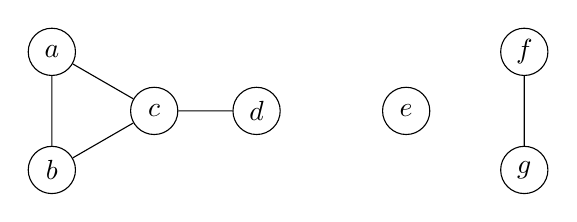
\begin{tikzpicture}[every node/.style={circle,draw,fill=white,inner sep=1.5pt,minimum size=6mm}]
\node (a) at (0,1.5) {$a$};
\node (b) at (0,0) {$b$};
\node (c) at (1.3,0.75) {$c$};
\node (d) at (2.6,0.75) {$d$};
\node (e) at (4.5,0.75) {$e$};
\node (f) at (6,1.5) {$f$};
\node (g) at (6,0) {$g$};
\draw (a)--(b) (a)--(c) (b)--(c) (c)--(d) (f)--(g);
\end{tikzpicture}
\end{center}
\begin{center}
\small $e$ is isolated; $d,f,g$ are leaves; $\{a,b,c,d\}$, $\{e\}$, $\{f,g\}$ are the three components (\S\ref{sec:11-9})
\end{center}

\begin{note}[Common graph models, Rosen \S10.1]
\emph{Acquaintanceship graph}: people as vertices, edge iff they know each other. \emph{Influence graph}: directed, edge $u\to v$ iff $u$ influences $v$. \emph{Call graph}: directed multigraph, edge per phone call. \emph{Precedence graph}: directed, edge $u\to v$ iff task $u$ must precede task $v$ (used in scheduling). \emph{Niche overlap graph}: species as vertices, edge iff they compete for the same food source.
\end{note}

\subsection{Types of graphs}
\label{sec:11-2}
% CN 11.2 / Rosen 10.1-10.2

\begin{definition}[Simple graph]
$G$ is \emph{simple} iff no loops (edge $\{v,v\}$) and no multiple edges.
\end{definition}

\begin{note}[Relaxations, Rosen's classification]
\emph{Multigraph}: multiple edges allowed. \emph{Pseudograph}: loops also allowed. \emph{Directed graph}: edges are ordered pairs $(v,w)\in V\times V$ (\emph{arcs}). \emph{Weighted graph}: each edge carries a number.
\end{note}

\begin{center}
\begin{tikzpicture}[every node/.style={circle,draw,fill=white,inner sep=1.5pt,minimum size=6mm}, >={Stealth[length=2mm]}]
\node (v1) at (0,0) {$v_1$};
\node (v2) at (2,0.8) {$v_2$};
\node (v3) at (2,-0.8) {$v_3$};
\node (v4) at (4,0) {$v_4$};
\draw[->] (v1)--(v2);
\draw[->] (v1)--(v3);
\draw[->] (v2)--(v4);
\draw[->] (v3)--(v4);
\draw[->] (v2) to[bend left] (v3);
\draw[->] (v4) to[out=150,in=210,looseness=8] (v4);
\end{tikzpicture}
\qquad
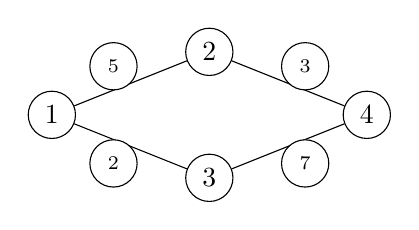
\begin{tikzpicture}[every node/.style={circle,draw,fill=white,inner sep=1.5pt,minimum size=6mm}]
\node (w1) at (0,0) {$1$};
\node (w2) at (2,0.8) {$2$};
\node (w3) at (2,-0.8) {$3$};
\node (w4) at (4,0) {$4$};
\draw (w1)--(w2) node[midway,above left,font=\scriptsize] {$5$};
\draw (w1)--(w3) node[midway,below left,font=\scriptsize] {$2$};
\draw (w2)--(w4) node[midway,above right,font=\scriptsize] {$3$};
\draw (w3)--(w4) node[midway,below right,font=\scriptsize] {$7$};
\end{tikzpicture}
\end{center}
\begin{center}
\small Directed graph (left, with a self-loop at $v_4$) and weighted graph (right)
\end{center}

\begin{definition}[Complement, Rosen]
For simple $G=(V,E)$: $\overline G=(V,\overline E)$, $\overline E=\{\{v,w\}: v\neq w,\ \{v,w\}\notin E\}$.
\end{definition}

\begin{definition}[Wheel graph, Rosen]
$W_n$: $C_n$ plus one hub vertex adjacent to all $n$ rim vertices.
\end{definition}

\begin{theorem}
\[
|E(\overline G)| = \binom n2 - |E(G)|.
\]
\end{theorem}

\subsection{Graphs and relations}
\label{sec:11-3}
% CN 11.3 (omega) / Rosen 9.1, 9.3

\begin{theorem}
Simple graphs correspond exactly to irreflexive symmetric binary relations.
\end{theorem}
\begin{proof}
Given simple $G=(V,E)$, define $R\subseteq V\times V$ by $(v,w)\in R\iff\{v,w\}\in E$. $R$ is irreflexive (no loops) and symmetric ($\{v,w\}=\{w,v\}$). Conversely, any irreflexive symmetric $R$ on $V$ gives $E=\{\{v,w\}:(v,w)\in R\}$, a simple graph.
\end{proof}

\begin{note}
Dropping irreflexivity allows loops; dropping symmetry gives directed graphs (\S\ref{sec:2-13}'s general relations, unrestricted).
\end{note}

\subsection{Representing graphs}
\label{sec:11-4}
% CN 11.4 / Rosen 10.3

\subsubsection{Edge list}
\begin{definition}
The list of all edges, $\{v,w\}$ pairs, explicitly.
\end{definition}

\subsubsection{Adjacency matrix}
\begin{definition}
For $V=\{v_1,\dots,v_n\}$: $A_{ij}=1$ if $v_i\sim v_j$, else $0$.
\end{definition}

\[
A =
\begin{pmatrix}
0 & 1 & 1 & 0 & 0 \\
1 & 0 & 1 & 0 & 0 \\
1 & 1 & 0 & 1 & 0 \\
0 & 0 & 1 & 0 & 0 \\
0 & 0 & 0 & 0 & 0
\end{pmatrix}
\]

\begin{center}
\small Adjacency matrix of \S\ref{sec:11-1}'s graph, restricted to $\{a,b,c,d,e\}$, in that vertex order -- row/column $5$ ($e$) all zero, matching that $e$ is isolated
\end{center}

\begin{note}
$A$ is symmetric (undirected); diagonal all $0$ (simple). Exactly \S\ref{sec:2-6}'s zero-one matrix of the adjacency relation.
\end{note}

\subsubsection{Adjacency list}
\begin{definition}
For each $v$, the list $N(v)$.
\end{definition}

\subsubsection{Incidence matrix}
\begin{definition}
For $V=\{v_1,\dots,v_n\}$, $E=\{e_1,\dots,e_m\}$: $M_{ij}=1$ if $v_i$ incident with $e_j$, else $0$.
\end{definition}
\begin{note}
Each column has exactly two $1$s (an edge has two endpoints).
\end{note}

\begin{theorem}[Counting walks via matrix powers, Rosen]
For adjacency matrix $A$ of $G$: $(A^r)_{ij}$ = number of length-$r$ walks from $v_i$ to $v_j$.
\end{theorem}
\begin{proof}[Induction on $r$]
\textbf{Base case} ($r=1$): $(A^1)_{ij}=A_{ij}\in\{0,1\}$ counts length-$1$ walks (edges) $v_i\to v_j$ correctly.

\textbf{Inductive step}: assume $(A^r)_{ij}$ counts length-$r$ walks. A length-$(r{+}1)$ walk $v_i\to v_j$ is a length-$r$ walk $v_i\to v_k$ followed by an edge $v_k\to v_j$, for some intermediate $v_k$:
\[
(A^{r+1})_{ij} = \sum_k (A^r)_{ik}A_{kj},
\]
exactly ordinary matrix multiplication, and exactly the count of length-$(r{+}1)$ walks (summing over all valid last-step choices $k$).
\end{proof}

\subsection{Graph isomorphism}
\label{sec:11-4-2}
% Rosen 10.3

\begin{definition}[Isomorphism]
$G_1=(V_1,E_1),\ G_2=(V_2,E_2)$ are \emph{isomorphic} iff $\exists$ bijection $f:V_1\to V_2$ with $\{u,v\}\in E_1 \iff \{f(u),f(v)\}\in E_2$.
\end{definition}

\begin{note}[Necessary invariants]
Isomorphic graphs agree on: $|V|$, $|E|$, degree sequence (sorted list of degrees), connectivity. Disagreement on any $\Rightarrow$ not isomorphic.
\end{note}

\begin{example}[Same degree sequence, not isomorphic -- harder]
Two graphs on $6$ vertices, both with degree sequence $(2,2,2,2,2,2)$: $C_6$ (one hexagon) vs.\ two disjoint copies of $C_3$. Not isomorphic ($C_6$ connected, the other isn't) -- degree sequence is necessary, not sufficient.
\end{example}

\begin{note}[Computational status, Rosen -- genuinely open]
No polynomial-time algorithm for graph isomorphism is known, yet it is also not known to be NP-complete -- one of very few natural problems whose complexity class remains unresolved (though quasi-polynomial algorithms exist, Babai 2015).
\end{note}

\subsection{Subgraphs}
\label{sec:11-5}
% CN 11.5 / Rosen 10.1

\begin{definition}[Subgraph]
$H=(V_H,E_H)$ is a \emph{subgraph} of $G=(V,E)$ iff $V_H\subseteq V$, $E_H\subseteq E$ (with $E_H$'s endpoints in $V_H$).
\end{definition}

\begin{definition}[Induced subgraph]
The subgraph \emph{induced} by $S\subseteq V$: vertices $S$, edges $\{v,w\}\in E$ with $v,w\in S$ (\emph{all} such edges).
\end{definition}

\begin{center}
\begin{tikzpicture}[every node/.style={circle,draw,fill=white,inner sep=1.5pt,minimum size=6mm}]
\node (p) at (0,1) {$p$};
\node (q) at (1.3,1.6) {$q$};
\node (r) at (1.3,0.4) {$r$};
\node (s) at (2.6,1) {$s$};
\draw[thick] (p)--(q) (p)--(r) (q)--(r) (q)--(s) (r)--(s);
\begin{scope}[on background layer]
\filldraw[fill=blue!10,draw=blue,rounded corners] (-0.5,0.2) rectangle (2,2.1);
\end{scope}
\end{tikzpicture}
\end{center}
\begin{center}
\small The subgraph induced by $\{p,q,r\}$ (shaded): includes \emph{every} edge among them, $\{p,q\},\{p,r\},\{q,r\}$ -- not just some
\end{center}

\subsection{Some special graphs}
\label{sec:11-6}
% CN 11.6 / Rosen 10.2

\begin{definition}[Standard families]
\[
K_n \text{ (complete)}: \text{every pair adjacent}. \qquad C_n \text{ (cycle)}: v_1\sim v_2\sim\cdots\sim v_n\sim v_1.
\]
\[
K_{m,n} \text{ (complete bipartite)}: V=A\sqcup B,\ |A|=m,|B|=n,\ v\sim w \iff v\in A, w\in B.
\]
\[
Q_n \text{ (hypercube)}: V=\{0,1\}^n,\ v\sim w \iff v,w \text{ differ in exactly one coordinate}.
\]
\end{definition}

\begin{theorem}
\[
|E(K_n)| = \binom n2, \qquad |E(Q_n)| = n\cdot2^{n-1}.
\]
\end{theorem}
\begin{proof}[$Q_n$ case]
Each vertex has degree $n$ (flip any one of $n$ coordinates); by \S\ref{sec:11-7}'s handshaking lemma, $|E|=\dfrac{n\cdot2^n}{2}=n2^{n-1}$.
\end{proof}

\begin{center}
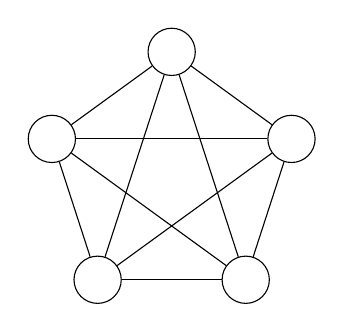
\begin{tikzpicture}[every node/.style={circle,draw,fill=white,inner sep=1.5pt,minimum size=6mm}]
\foreach \i in {0,...,4} {
  \node (v\i) at ({90+\i*72}:1.6) {};
}
\foreach \i in {0,...,4} {
  \foreach \j in {0,...,4} {
    \ifnum\i<\j
      \draw (v\i)--(v\j);
    \fi
  }
}
\end{tikzpicture}
\qquad
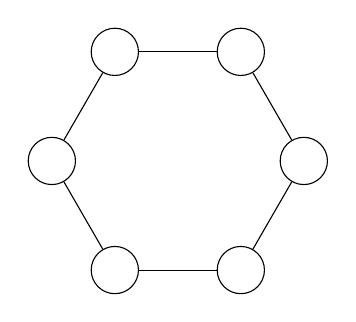
\begin{tikzpicture}[every node/.style={circle,draw,fill=white,inner sep=1.5pt,minimum size=6mm}]
\foreach \i in {0,...,5} {
  \node (c\i) at ({60*\i}:1.6) {};
}
\foreach \i in {0,...,5} {
  \pgfmathtruncatemacro{\j}{mod(\i+1,6)}
  \draw (c\i)--(c\j);
}
\end{tikzpicture}
\end{center}
\begin{center}
\small $K_5$ (left) and $C_6$ (right)
\end{center}

\begin{center}
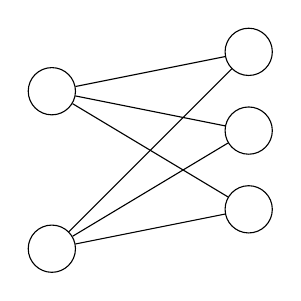
\begin{tikzpicture}[every node/.style={circle,draw,fill=white,inner sep=1.5pt,minimum size=6mm}]
\node (a1) at (0,1) {};
\node (a2) at (0,-1) {};
\node (b1) at (2.5,1.5) {};
\node (b2) at (2.5,0.5) {};
\node (b3) at (2.5,-0.5) {};
\foreach \a in {a1,a2} {
  \foreach \b in {b1,b2,b3} {
    \draw (\a)--(\b);
  }
}
\end{tikzpicture}
\qquad
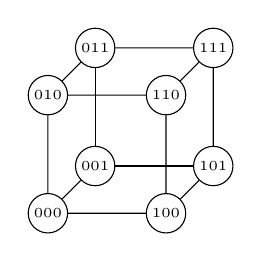
\begin{tikzpicture}[every node/.style={circle,draw,fill=white,inner sep=1pt,minimum size=5mm,font=\tiny}]
\node (000) at (0,0) {000};
\node (100) at (1.5,0) {100};
\node (010) at (0,1.5) {010};
\node (001) at (0.6,0.6) {001};
\node (110) at (1.5,1.5) {110};
\node (101) at (2.1,0.6) {101};
\node (011) at (0.6,2.1) {011};
\node (111) at (2.1,2.1) {111};
\draw (000)--(100) (000)--(010) (000)--(001);
\draw (100)--(110) (100)--(101);
\draw (010)--(110) (010)--(011);
\draw (001)--(101) (001)--(011);
\draw (110)--(111) (101)--(111) (011)--(111);
\end{tikzpicture}
\end{center}
\begin{center}
\small $K_{2,3}$ (left) and $Q_3$ (right)
\end{center}

\subsection{Degree}
\label{sec:11-7}
% CN 11.7 / Rosen 10.1

\begin{definition}[Degree]
$\deg(v) = |N(v)|$.
\end{definition}

\begin{theorem}[Handshaking lemma]
\[
\sum_{v\in V} \deg(v) = 2|E|.
\]
\end{theorem}
\begin{proof}
Each edge $\{v,w\}$ contributes exactly $1$ to $\deg(v)$ and $1$ to $\deg(w)$ -- $2$ total across the sum. Summing over all edges: $2|E|$.
\end{proof}

\begin{corollary}
The number of odd-degree vertices is even.
\end{corollary}
\begin{proof}
$\sum_v\deg(v)=2|E|$ is even. Split the sum over even- and odd-degree vertices: the even-degree part is automatically even, so the odd-degree part (a sum of odd numbers) must also be even -- forcing an even \emph{count} of odd terms.
\end{proof}

\bigskip
\begin{theorem}[Two vertices share a degree, CN Thm 56 -- proof by cases]
Every graph on $n\ge2$ vertices has two vertices of equal degree.
\end{theorem}
\begin{proof}
Possible degrees lie in $\{0,1,\dots,n-1\}$, $n$ values.

\textbf{Case 1}: no vertex has degree $n-1$. Then degrees lie in $\{0,\dots,n-2\}$, only $n-1$ values for $n$ vertices -- pigeonhole (\S\ref{sec:8-2}) forces a repeat.

\textbf{Case 2}: some vertex $v$ has degree $n-1$ (adjacent to all others). Then every other vertex has degree $\ge1$, so no vertex has degree $0$: degrees lie in $\{1,\dots,n-1\}$, again $n-1$ values for $n$ vertices -- pigeonhole forces a repeat.
\end{proof}

\subsection{Moving around}
\label{sec:11-8}
% CN 11.8 / Rosen 10.4

\begin{definition}[Walk, closed walk]
A \emph{walk} from $v$ to $w$: $v_0,v_1,\dots,v_k$ with $v_0=v,\ v_k=w$, each $v_{i-1}\sim v_i$. \emph{Length} $=k$. \emph{Closed} iff $v_0=v_k$.
\end{definition}

\begin{center}
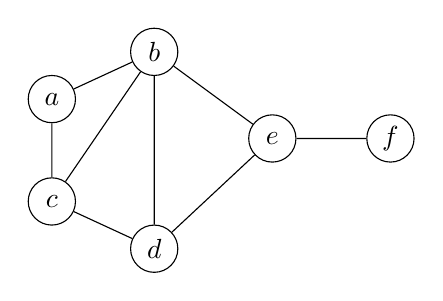
\begin{tikzpicture}[every node/.style={circle,draw,fill=white,inner sep=1.5pt,minimum size=6mm}]
\node (a) at (0,1) {$a$};
\node (b) at (1.3,1.6) {$b$};
\node (c) at (0,-0.3) {$c$};
\node (d) at (1.3,-0.9) {$d$};
\node (e) at (2.8,0.5) {$e$};
\node (f) at (4.3,0.5) {$f$};
\draw (a)--(b) (a)--(c) (b)--(c) (b)--(d) (c)--(d) (b)--(e) (d)--(e) (e)--(f);
\end{tikzpicture}
\end{center}
\begin{center}
\small $a,b,d,e,f$ is a walk of length $4$ (also a path); $a,b,c,a$ is a closed walk/cycle of length $3$
\end{center}

\begin{definition}[Trail, path, cycle]
A \emph{trail}: walk with no repeated edge. A \emph{path}: trail with no repeated vertex. A \emph{cycle}: closed trail with no repeated vertex except $v_0=v_k$.
\end{definition}

\begin{note}[Strictly increasing restriction]
\[
\text{walk} \supseteq \text{trail} \supseteq \text{path}.
\]
\end{note}

\begin{definition}[Distance]
$d(v,w)$ = length of the shortest path (equivalently, shortest walk) between $v,w$.
\end{definition}

\bigskip
\begin{theorem}[Odd closed walk $\iff$ odd cycle, CN Thm 60]
$G$ has an odd-length closed walk $\iff$ $G$ has an odd cycle.
\end{theorem}
\begin{proof}
($\Leftarrow$) Every cycle is a closed walk.

($\Rightarrow$) Let $W=v_0,\dots,v_k$ ($k$ odd) be the \emph{shortest} odd closed walk. If $W$ repeats no vertex besides $v_0=v_k$, $W$ is already an odd cycle.

Otherwise, suppose $v_i=v_j$ for some $0\le i<j\le k-1$. Split $W$ into two closed walks:
\[
v_i,\dots,v_j \qquad \text{and} \qquad v_j,\dots,v_{k-1},v_0,\dots,v_i.
\]
Their lengths sum to $k$ (odd), so one is odd, one even; the odd one is a shorter odd closed walk than $W$ -- contradicting minimality of $W$.

So $W$ has no repeated vertex besides $v_0=v_k$: $W$ is an odd cycle.
\end{proof}

\begin{note}[Fails for ``even'']
$K_2$: closed walk $v,w,v$ (even, length $2$) exists, but no cycle at all exists.
\end{note}

\begin{definition}[Hamiltonian cycle]
A cycle including every vertex of $G$.
\end{definition}

\begin{note}[Travelling Salesman Problem]
Finding a minimum-total-weight Hamiltonian cycle -- among the most famous NP-hard problems (\S\ref{sec:6-9}).
\end{note}

\subsection{Vertex and edge connectivity}
\label{sec:11-9-3}
% Rosen 10.4

\begin{definition}[Cut vertex, bridge]
$v$ is a \emph{cut vertex} iff $G-v$ has more components than $G$. $e$ is a \emph{bridge} iff $G-e$ does.
\end{definition}

\begin{theorem}
$e=\{u,v\}$ is a bridge $\iff$ $e$ lies on no cycle.
\end{theorem}

\begin{definition}[Vertex/edge connectivity, Rosen]
$\kappa(G)$ = minimum number of vertices whose removal disconnects $G$ (or leaves $1$ vertex). $\lambda(G)$ = minimum number of edges whose removal disconnects $G$.
\end{definition}

\begin{theorem}[Menger's theorem, Rosen -- harder]
For non-adjacent $s,t$: the maximum number of vertex-disjoint $s$-$t$ paths equals the minimum number of vertices whose removal disconnects $s$ from $t$.
\end{theorem}
\begin{note}
A cornerstone duality result (max-flow-min-cut's combinatorial ancestor); full proof beyond this course.
\end{note}

\bigskip
\begin{definition}[Strongly connected, Rosen -- directed graphs]
Directed $G$ is \emph{strongly connected} iff, for every $u,v$, a directed path exists $u\to v$ \emph{and} $v\to u$.
\end{definition}

\begin{definition}[Strongly connected component]
A maximal strongly-connected subgraph.
\end{definition}

\begin{note}
Unlike undirected components (\S\ref{sec:11-9}), a directed graph's strongly connected components can have edges \emph{between} them (one-directional) -- they don't simply "partition into isolated pieces" the way undirected components do.
\end{note}

\subsection{Shortest paths}
\label{sec:11-9-4}
% Rosen 10.6

\begin{definition}[Shortest path problem]
For weighted $G$, $w:E\to\R^+$: find, for source $s$, the minimum-weight path to each other vertex.
\end{definition}

\begin{algorithm}[H]
\SetAlgoLined
\KwIn{Weighted graph $G=(V,E,w)$, source $s$}
\KwOut{$d[v]=$ shortest distance from $s$ to every $v$}
$d[s]\gets0$\;
\ForEach{$v\in V\setminus\{s\}$}{$d[v]\gets\infty$}
$S\gets\emptyset$\;
\While{$S\neq V$}{
    $u\gets\arg\min_{v\notin S} d[v]$\;
    $S\gets S\cup\{u\}$\;
    \ForEach{neighbour $v$ of $u$}{
        \If{$d[u]+w(u,v) < d[v]$}{
            $d[v]\gets d[u]+w(u,v)$\;
        }
    }
}
\caption{Dijkstra's algorithm}
\end{algorithm}

\begin{theorem}[Correctness]
When $u$ is added to $S$, $d[u]$ is $u$'s true shortest distance from $s$.
\end{theorem}
\begin{proof}[Proof sketch, induction on $|S|$]
Suppose true for all previously-added vertices. Suppose $d[u]$ were not the true shortest distance -- some shorter $s$-$u$ path $P$ exists. $P$ must leave $S$ at some point, at edge $x\to y$ ($x\in S, y\notin S$). Since edge weights are positive, the portion of $P$ up to $y$ already has length $\ge d[y]$ (by relaxation via $x$, whose distance was already correct by the inductive hypothesis), and the rest of $P$ from $y$ to $u$ adds more positive weight -- so $P$'s total length is $\ge d[y] \ge d[u]$ (since $u$ was chosen as the minimum $d$-value not yet in $S$), contradicting $P$ being shorter.
\end{proof}

\begin{note}[Complexity]
Naive implementation: $O(n)$ to find the minimum each round, $n$ rounds: $O(n^2)$ (\S\ref{sec:6-9}). A priority-queue implementation improves this to $O((n+m)\log n)$.
\end{note}

\begin{example}[Why Dijkstra fails with negative weights -- harder]
$s\to a$ weight $1$, $s\to b$ weight $4$, $a\to b$ weight $-3$. Dijkstra finalizes $a$ first ($d[a]=1$), then $s$ or $a$ next by tentative distance; but it finalizes $s\to b$ directly at $4$ before ever relaxing via $a$ (since $a$'s $d$-value $1<4$, $a$ is chosen \emph{before} $b$ is finalized -- actually here it does relax correctly). A cleaner failing example: $s\to a$ weight $2$, $s\to b$ weight $1$, $b\to a$ weight $-2$: Dijkstra finalizes $b$ first ($d=1$), relaxes $a$ to $\min(2,1-2)=-1$ correctly here too -- but if $b$ had been finalized \emph{before} discovering a cheaper route via a vertex not yet reached, that finalized value can never be revisited. In general: once a vertex is finalized, Dijkstra never revisits it, so a later-discovered negative-weight shortcut into an already-finalized vertex is missed entirely.
\end{example}

\begin{note}[Unweighted case reduces to BFS]
When all weights equal $1$: Dijkstra's "always expand the nearest unfinalized vertex" is exactly breadth-first search (\S\ref{sec:12-4}) -- BFS suffices, no priority queue needed.
\end{note}

\subsection{Connectivity}
\label{sec:11-9}
% CN 11.9 / Rosen 10.4

\begin{definition}[Connected graph, component]
$v,w$ are \emph{connected} iff a path (equivalently, walk) joins them. $G$ is \emph{connected} iff every pair is. A \emph{component} is a maximal connected subgraph.
\end{definition}

\begin{theorem}
Connectivity is an equivalence relation on $V$; its equivalence classes are exactly the vertex sets of $G$'s components.
\end{theorem}
\begin{proof}
Reflexive: length-$0$ walk. Symmetric: reverse a walk. Transitive: concatenate walks at the shared vertex. By \S\ref{sec:2-16}'s theorem, equivalence classes partition $V$.
\end{proof}

\begin{center}
\begin{tikzpicture}[every node/.style={circle,draw,fill=white,inner sep=1.5pt,minimum size=6mm}]
\node (a) at (0,1.5) {$a$};
\node (b) at (0,0) {$b$};
\node (c) at (1.3,0.75) {$c$};
\node (d) at (2.6,0.75) {$d$};
\node (e) at (4.5,0.75) {$e$};
\node (f) at (6,1.5) {$f$};
\node (g) at (6,0) {$g$};
\draw (a)--(b) (a)--(c) (b)--(c) (c)--(d) (f)--(g);
\begin{scope}[on background layer]
\filldraw[fill=blue!10,draw=blue,rounded corners] (-0.6,-0.6) rectangle (3.2,2.1);
\filldraw[fill=red!10,draw=red,rounded corners] (4.1,0.35) rectangle (4.9,1.15);
\filldraw[fill=green!10,draw=green!50!black,rounded corners] (5.5,-0.6) rectangle (6.5,2.1);
\end{scope}
\end{tikzpicture}
\end{center}
\begin{center}
\small The three components of \S\ref{sec:11-1}'s graph -- each shaded region is one equivalence class
\end{center}

\subsection{Bipartite graphs}
\label{sec:11-10}
% CN 11.10 / Rosen 10.2

\begin{definition}[Bipartite]
$G$ is \emph{bipartite} iff $V=A\sqcup B$ with every edge having one endpoint in each part.
\end{definition}

\begin{definition}[$2$-colouring]
A function $V\to\{\text{Black,White}\}$ with adjacent vertices differently coloured.
\end{definition}

\begin{center}
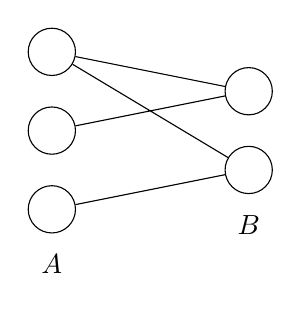
\begin{tikzpicture}[every node/.style={circle,draw,fill=white,inner sep=1.5pt,minimum size=6mm}]
\node (a1) at (0,1.5) {};
\node (a2) at (0,0.5) {};
\node (a3) at (0,-0.5) {};
\node (b1) at (2.5,1) {};
\node (b2) at (2.5,0) {};
\draw (a1)--(b1) (a1)--(b2) (a2)--(b1) (a3)--(b2);
\node[draw=none,fill=none] at (0,-1.2) {$A$};
\node[draw=none,fill=none] at (2.5,-0.7) {$B$};
\end{tikzpicture}
\end{center}
\begin{center}
\small A bipartite graph: every edge crosses between $A$ and $B$
\end{center}

\begin{theorem}
$G$ bipartite $\iff$ $G$ has a $2$-colouring.
\end{theorem}
\begin{proof}
($\Rightarrow$) Colour $A$ Black, $B$ White; every edge crosses parts, so is Black-White.

($\Leftarrow$) Given $2$-colouring $f$, let $A=f^{-1}(\text{Black}),\ B=f^{-1}(\text{White})$: a partition (\S\ref{sec:1-15}), and every edge connects differently-coloured, hence differently-partitioned, vertices.
\end{proof}

\bigskip
\begin{theorem}[Bipartite $\iff$ no odd closed walk]
$G$ bipartite $\iff$ $G$ has no odd-length closed walk.
\end{theorem}
\begin{proof}
($\Rightarrow$) In a bipartite graph, every walk alternates $A,B,A,B,\dots$; returning to the start after $k$ steps requires $k$ even.

($\Leftarrow$) In each component, fix a ground vertex $g$; colour $v$ Black if $d(g,v)$ even, White if odd. If some edge $\{v,w\}$ had $v,w$ same colour, $d(g,v),d(g,w)$ have equal parity, so a shortest-$g$-$v$-path, plus edge $\{v,w\}$, plus a shortest-$w$-$g$-path forms a closed walk of length $d(g,v)+d(g,w)+1$ -- odd (even $+$ even $+1$, or odd$+$odd$+1$) -- contradicting the hypothesis. So no such edge exists: this coloring is a valid $2$-colouring.
\end{proof}

\begin{corollary}
$G$ bipartite $\iff$ $G$ has no odd cycle.
\end{corollary}
\begin{proof}
Combine with \S\ref{sec:11-8}'s odd-closed-walk-$\iff$-odd-cycle theorem.
\end{proof}

\subsection{Euler tours}
\label{sec:11-11}
% CN 11.11 / Rosen 10.5

\begin{definition}[Euler tour]
A closed trail using every edge exactly once.
\end{definition}

\begin{theorem}[Euler, 1736 -- Seven Bridges of Königsberg]
A connected graph $G$ has an Euler tour $\iff$ every vertex has even degree.
\end{theorem}
\begin{proof}
($\Rightarrow$) Every vertex-visit in a trail uses one incoming and one outgoing edge -- $2$ edges per visit, so each vertex's incident-edge count is even.

($\Leftarrow$) Algorithm: start a trivial closed trail $T$ at any vertex. While unused edges remain: find $v\in T$ with an unused incident edge (exists, since $G$ connected -- any unused edge's component meets $T$ somewhere, by connectivity); build a new closed trail $U$ from $v$ using only unused edges (possible at every step since $T$'s even-degree property leaves an even, hence nonzero-if-nonempty, number of unused edges at each vertex encountered); splice $U$ into $T$ at $v$. Terminates (finite edges), and every edge gets used exactly once.
\end{proof}

\begin{note}[Königsberg]
Modelled the four landmasses as vertices, seven bridges as edges: each vertex has odd degree ($3$ or $5$), so by the theorem no Euler tour exists -- resolving the centuries-old puzzle.
\end{note}

\begin{center}
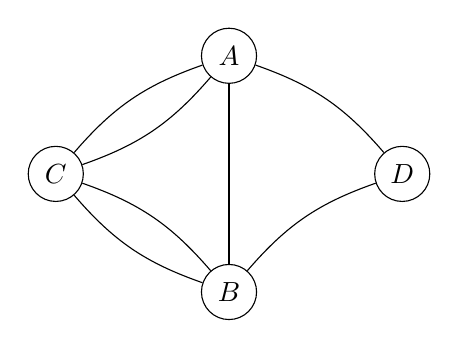
\begin{tikzpicture}[every node/.style={circle,draw,fill=white,inner sep=1.5pt,minimum size=7mm}]
\node (A) at (0,1.5) {$A$};
\node (B) at (0,-1.5) {$B$};
\node (C) at (-2.2,0) {$C$};
\node (D) at (2.2,0) {$D$};
\draw (A) to[bend left=15] (C);
\draw (A) to[bend right=15] (C);
\draw (B) to[bend left=15] (C);
\draw (B) to[bend right=15] (C);
\draw (A) to[bend left=15] (D);
\draw (B) to[bend left=15] (D);
\draw (A)--(B);
\end{tikzpicture}
\end{center}
\begin{center}
\small Königsberg bridges graph: $\deg(A)=\deg(B)=\deg(D)=3$ (odd), $\deg(C)=5$ (odd) -- all four vertices odd, so no Euler tour exists
\end{center}

\begin{note}[Extends to multigraphs/pseudographs]
Holds with multiple edges; loops count $2$ toward their vertex's degree.
\end{note}

\bigskip
\begin{theorem}[Route inspection / Chinese postman, Rosen -- harder extension]
If $G$ connected with $2k$ odd-degree vertices ($k\ge1$; even by \S\ref{sec:11-7}'s corollary), pairing them off and adding $k$ new edges (one per pair, parallel edges allowed) makes every degree even, giving an Euler tour of the augmented graph.
\end{theorem}
\begin{note}
Minimizing the total added length (pairing odd vertices via shortest paths to minimize duplicated edges) is the \emph{route inspection problem} -- unlike TSP (\S\ref{sec:11-8}), this is solvable in polynomial time via minimum-weight perfect matching.
\end{note}

\newpage
\section{Graph Theory II}

\subsection{Trees}
\label{sec:12-1}
% CN 12.1 / Rosen 11.1

\begin{definition}[Tree]
A \emph{tree} is a connected graph with no cycles.
\end{definition}

\begin{note}[Applications]
Communication networks (minimal connectivity), hierarchies (directories, class inheritance under single inheritance, org charts), decision trees, parse trees, rooted trees (a distinguished root, e.g.\ Unix's \texttt{/}).
\end{note}

\begin{center}
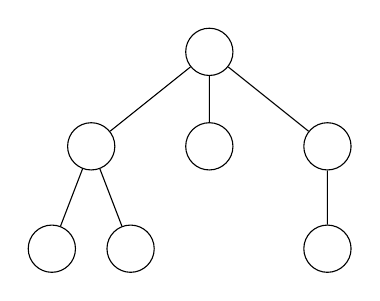
\begin{tikzpicture}[every node/.style={circle,draw,fill=white,inner sep=1.5pt,minimum size=6mm}]
\node (r) at (2,3) {};
\node (a) at (0.5,1.8) {};
\node (b) at (2,1.8) {};
\node (c) at (3.5,1.8) {};
\node (d) at (0,0.5) {};
\node (e) at (1,0.5) {};
\node (f) at (3.5,0.5) {};
\draw (r)--(a) (r)--(b) (r)--(c) (a)--(d) (a)--(e) (c)--(f);
\end{tikzpicture}
\end{center}
\begin{center}
\small A tree
\end{center}

\subsection{Equivalent characterizations of trees}
\label{sec:12-1-2}
% Rosen 11.1 -- summary theorem

\begin{theorem}[Rosen -- TFAE]
For a graph $G$ with $n$ vertices, the following are equivalent:
\begin{enumerate}[label=(\roman*)]
    \item $G$ is a tree.
    \item $G$ is connected and acyclic.
    \item $G$ is connected with $n-1$ edges.
    \item $G$ is acyclic with $n-1$ edges.
    \item $G$ is connected, and every edge is a bridge.
    \item Every pair of vertices is joined by a unique path.
    \item $G$ is acyclic, but adding any one edge creates exactly one cycle.
\end{enumerate}
\end{theorem}
\begin{note}
Each pairwise equivalence traces back to results already proved: (i)$\Leftrightarrow$(ii) is the definition; (ii)$\Leftrightarrow$(v) is \S\ref{sec:12-2}'s minimal-connected theorem; (ii)$\Rightarrow$(iii) and (ii)$\Rightarrow$(iv) use \S\ref{sec:12-2}'s edge-count theorem; (ii)$\Leftrightarrow$(vi) was noted after that theorem.
\end{note}

\subsection{Properties of trees}
\label{sec:12-2}
% CN 12.2 / Rosen 11.1-11.3

\begin{definition}[Minimal connected graph]
$G=(V,E)$ connected, but deleting \emph{any} edge disconnects it.
\end{definition}

\begin{theorem}[CN Thm 66]
$G$ is a tree $\iff$ $G$ is a minimal connected graph on $V$.
\end{theorem}
\begin{proof}
($\Rightarrow$) Let $G$ be a tree, and suppose (for contradiction) some edge $e=\{v,w\}$ can be deleted without disconnecting $G$. Then a $v$-$w$ path avoiding $e$ exists; adding $e$ back creates a cycle -- contradicting $G$ acyclic.

($\Leftarrow$) $G$ minimal connected; suppose (for contradiction) $G$ has a cycle $C$, edge $e\in C$. For any $v,w\in V$: any walk using $e$ can detour around the rest of $C$ instead, giving a walk avoiding $e$. So $G-e$ is still connected on the same vertex set -- contradicting minimality.
\end{proof}

\begin{note}[Unique paths]
Consequently, every pair of vertices in a tree is joined by a \emph{unique} path.
\end{note}

\begin{note}[Extremes among trees, $n$ vertices]
Path $P_{n-1}$: longest possible path ($n-1$), lowest possible max-degree ($2$). Star $K_{1,n-1}$: shortest possible paths (length $\le2$), highest possible max-degree ($n-1$).
\end{note}

\begin{center}
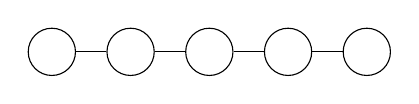
\begin{tikzpicture}[every node/.style={circle,draw,fill=white,inner sep=1.5pt,minimum size=6mm}]
\node (p1) at (0,0) {};
\node (p2) at (1,0) {};
\node (p3) at (2,0) {};
\node (p4) at (3,0) {};
\node (p5) at (4,0) {};
\draw (p1)--(p2)--(p3)--(p4)--(p5);
\end{tikzpicture}
\qquad
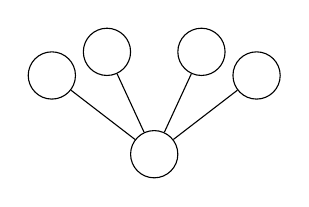
\begin{tikzpicture}[every node/.style={circle,draw,fill=white,inner sep=1.5pt,minimum size=6mm}]
\node (s0) at (0,0) {};
\node (s1) at (-1.3,1) {};
\node (s2) at (-0.6,1.3) {};
\node (s3) at (0.6,1.3) {};
\node (s4) at (1.3,1) {};
\draw (s0)--(s1) (s0)--(s2) (s0)--(s3) (s0)--(s4);
\end{tikzpicture}
\end{center}
\begin{center}
\small $P_4$ (left) and $K_{1,4}$ (right) -- the two extreme trees on $5$ vertices
\end{center}

\bigskip
\begin{theorem}[CN Thm 67]
Every tree with $\ge2$ vertices has a leaf.
\end{theorem}

\begin{theorem}[CN Thm 68 -- edge count]
Every tree on $n$ vertices has $n-1$ edges.
\end{theorem}
\begin{proof}[Induction on $n$]
\textbf{Base case} ($n=1$): the single-vertex tree has $0=1-1$ edges.

\medskip
\textbf{Inductive step}: let $k\ge1$; assume every $k$-vertex tree has $k-1$ edges. Let $T$ have $k+1$ vertices. By the leaf theorem, $T$ has a leaf $\ell$; let $S=T-\ell$ (delete $\ell$ and its one incident edge).

$S$ is still a tree (removing a leaf disconnects nothing, creates no cycle), with $k$ vertices -- so by the inductive hypothesis, $S$ has $k-1$ edges. $T$ has exactly one more edge than $S$ (the deleted one), so $T$ has $(k-1)+1=k$ edges.

\medskip
By induction, every $n$-vertex tree has $n-1$ edges.
\end{proof}

\bigskip
\begin{note}[Applications of trees, Rosen \S11.2 -- extension]
\emph{Binary search trees}: each node has $\le2$ children, left subtree smaller, right larger -- search, insert in $O(\log n)$ for balanced trees. \emph{Huffman coding}: build an optimal prefix-free binary code by repeatedly merging the two least-frequent symbols into a subtree, symbol frequency $\to$ leaf depth (frequent symbols get short codes). \emph{Decision trees}: each internal node a test, each leaf an outcome -- used to prove lower bounds on comparison-based algorithms (\S\ref{sec:6-9}).
\end{note}

\begin{definition}[Ordered rooted tree, binary tree, Rosen]
A \emph{rooted tree} has a distinguished root; children of each node are the tree's neighbours farther from the root. An \emph{ordered} rooted tree ranks each node's children (first, second, \dots). A \emph{binary tree}: every node has $\le2$ children, distinguished as left/right.
\end{definition}

\begin{note}[Tree traversals, Rosen \S11.3 -- harder]
For a binary tree with root $r$, left subtree $T_L$, right subtree $T_R$:
\[
\text{preorder}: r,\ \mathrm{pre}(T_L),\ \mathrm{pre}(T_R); \qquad
\text{inorder}: \mathrm{in}(T_L),\ r,\ \mathrm{in}(T_R); \qquad
\text{postorder}: \mathrm{post}(T_L),\ \mathrm{post}(T_R),\ r.
\]
\end{note}

\begin{example}[Expression tree, Rosen -- harder]
$(3+4)\times(5-2)$ as a binary tree: root $\times$, left subtree $+$ with leaves $3,4$, right subtree $-$ with leaves $5,2$.
\[
\text{preorder: } \times,+,3,4,-,5,2 \ \text{(prefix/Polish notation)}
\]
\[
\text{inorder: } 3,+,4,\times,5,-,2 \ \text{(infix, matches ordinary notation up to parentheses)}
\]
\[
\text{postorder: } 3,4,+,5,2,-,\times \ \text{(postfix/reverse Polish notation -- directly stack-evaluable)}
\]
\end{example}

\begin{definition}[Prefix code, Rosen]
A binary code where no codeword is a prefix of another -- guarantees unambiguous decoding of concatenated codewords.
\end{definition}

\begin{note}[Correspondence with binary trees]
A prefix code corresponds to a binary tree: each codeword is the path (L/R) from root to a leaf, symbols only at leaves.
\end{note}

\begin{theorem}[Kraft's inequality]
A prefix code with codeword lengths $l_1,\dots,l_k$ exists $\iff$
\[
\sum_{i=1}^k 2^{-l_i} \le 1.
\]
\end{theorem}

\bigskip
\begin{definition}[Huffman coding, Rosen]
Repeatedly merge the two least-frequent symbols/subtrees into a new subtree (frequency = sum), until one tree remains; codeword = root-to-leaf path.
\end{definition}

\begin{theorem}[Huffman coding is optimal]
Among all prefix codes, Huffman's construction minimizes expected codeword length $\sum_i f_i l_i$.
\end{theorem}
\begin{proof}[Proof sketch, exchange argument]
In an optimal tree, the two least-frequent symbols can always be assumed siblings at maximum depth (swapping any other arrangement to make this so never increases cost). Merging them into one symbol (frequency summed) and solving the smaller $(k-1)$-symbol problem optimally, by induction, then splitting back out, reproduces exactly Huffman's greedy merge -- so the greedy construction is optimal at every step.
\end{proof}

\bigskip
\begin{theorem}[Decision-tree lower bound for comparison sorts, Rosen -- harder]
Any comparison-based sorting algorithm needs $\Omega(n\log n)$ comparisons in the worst case.
\end{theorem}
\begin{proof}
Model the algorithm as a binary decision tree: each internal node one comparison, each leaf one possible output permutation. There are $n!$ possible orderings of $n$ distinct elements, each needing its own leaf, so the tree has $\ge n!$ leaves. A binary tree with $\ge n!$ leaves has depth $\ge\log_2(n!)$ (a depth-$d$ binary tree has $\le2^d$ leaves). By Stirling's approximation, $\log_2(n!) = \Theta(n\log n)$. The worst-case number of comparisons is the tree's depth, so $\ge\Omega(n\log n)$.
\end{proof}

\bigskip
\begin{note}[Game trees, Rosen -- minimax, extension]
A two-player game's positions form a tree: root = start, children = legal moves, leaves = terminal positions with a score. \emph{Minimax}: leaves scored from one player's perspective; internal nodes alternately take $\max$ (that player's turn) or $\min$ (opponent's turn) over children, propagating optimal-play values up to the root.
\end{note}

\begin{example}[Tic-tac-toe fragment]
At a node where X is about to move with two available squares leading to a forced win and a forced draw: X (maximizing) picks the win -- the max-node's value is "win," inherited from whichever child gives the best outcome for X.
\end{example}

\begin{definition}[Universal address system, Rosen]
Root labelled $0$; a node's $i$-th child (left to right) appends $.i$ to the parent's label ($1.2$: second child of the first child of the root).
\end{definition}

\begin{note}
Gives a canonical way to compare/order any two nodes (lexicographic order on labels) -- exactly the ordering that preorder traversal (\S\ref{sec:12-2}) visits nodes in.
\end{note}

\subsection{Forests}
\label{sec:12-3}
% CN 12.3 / Rosen 11.1

\begin{definition}[Forest]
A graph with no cycles (not necessarily connected).
\end{definition}

\begin{note}
Each component of a forest is itself connected and acyclic -- hence a tree. A forest is exactly a disjoint union of trees.
\end{note}

\begin{theorem}[CN Thm 69]
A forest with $n$ vertices and $k$ components has $n-k$ edges.
\end{theorem}
\begin{proof}
Let $F_1,\dots,F_k$ be the components, $n_i,m_i$ their vertex/edge counts. Then $n=\sum_i n_i$, $m=\sum_i m_i$, and each $F_i$ (a tree) has $m_i=n_i-1$ (\S\ref{sec:12-2}). So
\[
m = \sum_{i=1}^k m_i = \sum_{i=1}^k (n_i-1) = \sum_{i=1}^k n_i - k = n-k.
\]
\end{proof}

\begin{center}
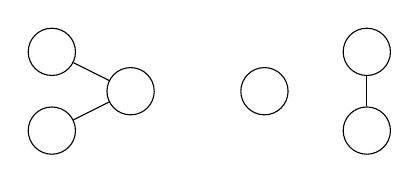
\begin{tikzpicture}[every node/.style={circle,draw,fill=white,inner sep=1.5pt,minimum size=6mm}]
\node (a) at (0,1) {}; \node (b) at (0,0) {}; \node (c) at (1,0.5) {};
\draw (a)--(c) (b)--(c);
\node (e) at (2.7,0.5) {};
\node (f) at (4,1) {}; \node (g) at (4,0) {};
\draw (f)--(g);
\end{tikzpicture}
\end{center}
\begin{center}
\small A forest with $3$ components (trees): $6$ vertices, $3$ edges $=n-k$
\end{center}

\subsection{Spanning tree algorithms}
\label{sec:12-4-2}
% Rosen 11.4-11.5

\begin{algorithm}[H]
\SetAlgoLined
\KwIn{Graph $G=(V,E)$, start vertex $s$}
\KwOut{Spanning tree $T$ of $s$'s component}
mark $s$ visited\; $T\gets(\{s\},\emptyset)$\;
\SetKwProg{Fn}{Function}{:}{}
\Fn{$\mathrm{DFS}(u)$}{
    \ForEach{neighbour $v$ of $u$}{
        \If{$v$ not visited}{
            mark $v$ visited\;
            add $v$ to $T$'s vertices, edge $\{u,v\}$ to $T$'s edges\;
            $\mathrm{DFS}(v)$\;
        }
    }
}
call $\mathrm{DFS}(s)$\;
\caption{Depth-first search}
\end{algorithm}

\begin{note}[Backtracking algorithms, Rosen -- application]
DFS underlies \emph{backtracking}: explore a choice, recurse; if a dead end (constraint violated) is reached, undo and try the next choice. This is exactly how a constraint-satisfaction search (e.g.\ the $n$-queens problem, \S\ref{sec:4-17}) can be solved directly, as an alternative to encoding it as SAT and calling a solver.
\end{note}

\bigskip
\begin{algorithm}[H]
\SetAlgoLined
\KwIn{Graph $G=(V,E)$, start vertex $s$}
\KwOut{Spanning tree $T$ of $s$'s component}
mark $s$ visited\; $T\gets(\{s\},\emptyset)$\; $Q\gets$ queue containing $s$\;
\While{$Q$ not empty}{
    $u\gets Q.\mathrm{dequeue}()$\;
    \ForEach{neighbour $v$ of $u$}{
        \If{$v$ not visited}{
            mark $v$ visited\;
            add $v$ to $T$'s vertices, edge $\{u,v\}$ to $T$'s edges\;
            $Q.\mathrm{enqueue}(v)$\;
        }
    }
}
\caption{Breadth-first search}
\end{algorithm}

\begin{theorem}[BFS solves unweighted shortest paths]
In BFS from $s$, each vertex $v$ is first discovered at exactly $d(s,v)$ (graph distance, \S\ref{sec:11-8}).
\end{theorem}
\begin{proof}[Proof sketch]
Induction on distance $k$: BFS discovers exactly the distance-$k$ vertices at level $k$, since it exhausts all distance-$(k{-}1)$ vertices' neighbours before any distance-$(k{+}1)$ vertex is reached.
\end{proof}

\bigskip
\begin{algorithm}[H]
\SetAlgoLined
\KwIn{Weighted connected graph $G=(V,E,w)$}
\KwOut{Minimum spanning tree $T$}
pick any $s\in V$\; $T\gets(\{s\},\emptyset)$\;
\While{$T$'s vertex set $\neq V$}{
    $e\gets$ minimum-weight edge with exactly one endpoint in $T$'s vertices\;
    add $e$'s edge and its outside endpoint to $T$\;
}
\caption{Prim's algorithm}
\end{algorithm}

\begin{theorem}[Prim's algorithm is optimal]
\end{theorem}
\begin{proof}[Proof sketch, cut property]
At each step, the chosen minimum-weight edge crosses the "cut" between $T$'s current vertices and the rest -- and the minimum-weight edge crossing any cut is always part of \emph{some} MST (if it weren't, swapping it into any MST for whatever edge does cross that cut, at no greater cost, produces another valid MST) -- so greedily taking it never rules out optimality.
\end{proof}

\subsection{Graph colouring}
\label{sec:12-5-2}
% Rosen 10.8

\begin{definition}[Chromatic number]
$\chi(G)$ = minimum $k$ such that $G$ has a proper $k$-colouring (adjacent vertices differ).
\end{definition}

\begin{theorem}[Greedy upper bound]
\[
\chi(G) \le \Delta(G)+1,
\]
where $\Delta(G)=\max_v\deg(v)$.
\end{theorem}
\begin{proof}
Order vertices arbitrarily; colour each in turn with the smallest colour not used by its already-coloured neighbours. Each vertex has $\le\Delta(G)$ neighbours, so some colour among $\{1,\dots,\Delta(G)+1\}$ is always free.
\end{proof}

\begin{theorem}
\[
\chi(G) = 2 \iff G \text{ bipartite} \iff G \text{ has no odd cycle}
\]
(restating \S\ref{sec:11-10}'s theorem in colouring language).
\end{theorem}

\begin{example}[Applications, Rosen]
\emph{Exam/course scheduling}: courses as vertices, edge iff they share a student -- colours = time slots, proper colouring avoids conflicts. \emph{Frequency assignment}: transmitters as vertices, edge iff they'd interfere -- colours = frequencies.
\end{example}

\begin{note}
$\chi(G)\le4$ for every planar $G$ (\S\ref{sec:12-5}'s four colour theorem) -- but computing $\chi(G)$ exactly, for general graphs, is NP-hard.
\end{note}

\subsection{Spanning trees}
\label{sec:12-4}
% CN 12.4 / Rosen 11.4-11.5

\begin{definition}[Spanning tree]
A subgraph of connected $G$ that is a tree and includes every vertex of $G$.
\end{definition}

\begin{theorem}[Existence]
Every connected graph has a spanning tree.
\end{theorem}

\begin{algorithm}[H]
\SetAlgoLined
\KwIn{Connected graph $G=(V,E)$}
\KwOut{Spanning tree $F=(V,X)$}
$X\gets\emptyset$\;
\While{$\exists e\in E\setminus X$ such that $X\cup\{e\}$ is acyclic}{
    pick such an $e$\;
    $X\gets X\cup\{e\}$\;
}
\caption{Spanning tree via edge addition}
\end{algorithm}

\begin{proof}[Correctness of the algorithm above]
$F$ is acyclic by construction (a forest). $F$ is connected: if not, some component boundary edge of $G$ could be added to $X$ without creating a cycle (endpoints in different components), contradicting termination. So $F$ is a connected forest -- a tree -- spanning $V$.
\end{proof}

\begin{center}
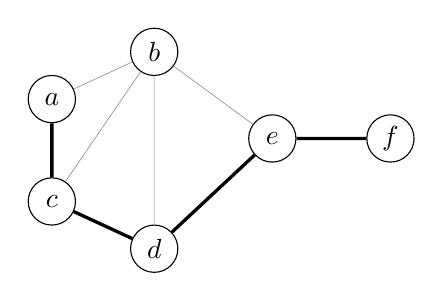
\begin{tikzpicture}[every node/.style={circle,draw,fill=white,inner sep=1.5pt,minimum size=6mm}]
\node (a) at (0,1) {$a$};
\node (b) at (1.3,1.6) {$b$};
\node (c) at (0,-0.3) {$c$};
\node (d) at (1.3,-0.9) {$d$};
\node (e) at (2.8,0.5) {$e$};
\node (f) at (4.3,0.5) {$f$};
\draw[very thin, gray] (a)--(b) (b)--(c) (b)--(d) (c)--(d) (b)--(e);
\draw[very thick] (a)--(c) (c)--(d) (d)--(e) (e)--(f);
\end{tikzpicture}
\end{center}
\begin{center}
\small A spanning tree (thick edges) of \S\ref{sec:11-8}'s example graph
\end{center}

\bigskip
\begin{definition}[Minimum spanning tree]
For weighted connected $G$: a spanning tree minimizing $w(X)=\sum_{e\in X}w(e)$.
\end{definition}

\begin{algorithm}[H]
\SetAlgoLined
\KwIn{Weighted connected graph $G=(V,E,w)$}
\KwOut{Minimum spanning tree $F=(V,X)$}
$X\gets\emptyset$\;
sort $E$ by increasing weight\;
\ForEach{$e\in E$, in sorted order}{
    \If{$X\cup\{e\}$ is acyclic}{
        $X\gets X\cup\{e\}$\;
    }
}
\caption{Kruskal's algorithm}
\end{algorithm}

\begin{theorem}[Kruskal's algorithm is optimal, CN Thm 70]
Kruskal's algorithm produces a minimum spanning tree.
\end{theorem}
\begin{note}[Proof idea -- the exchange argument, Rosen -- harder]
Suppose Kruskal's tree $T$ is not minimum; let $T^*$ be a minimum spanning tree agreeing with $T$ on as many edges as possible, and let $e$ be the first edge Kruskal chose that is \emph{not} in $T^*$. Adding $e$ to $T^*$ creates a cycle $C$; since $T^*$ is a tree, $C$ has some edge $f\notin T$ (else $T$ itself would contain a cycle). Since Kruskal chose $e$ before considering $f$ (or never needed $f$, having already connected those components via earlier, no-more-expensive edges), $w(e)\le w(f)$. Swapping: $T^{**}=T^*-f+e$ is also a spanning tree, with $w(T^{**})\le w(T^*)$ (so still minimum), and agrees with $T$ on strictly more edges -- contradicting the choice of $T^*$. So no such $e$ exists: $T=T^*$.
\end{note}

\begin{note}[Prim's algorithm, Rosen -- alternate greedy MST algorithm]
Grow a single tree from one starting vertex: repeatedly add the minimum-weight edge connecting the current tree to a new vertex (rather than Kruskal's "cheapest edge anywhere, cycle permitting"). Also provably optimal, by a similar exchange argument.
\end{note}

\begin{note}[Why greedy is exceptional here]
Greedy algorithms rarely give optimal solutions in general (e.g.\ greedy shortest-path search can fail badly, \S\ref{sec:6-9}'s complexity themes). MST is a striking exception -- the underlying reason (the ``matroid'' structure of forests) is studied in \emph{matroid theory}, which characterizes exactly when greedy algorithms are guaranteed optimal.
\end{note}

\subsection{Planarity}
\label{sec:12-5}
% CN 12.5 / Rosen 10.7-10.8

\begin{definition}[Planar graph]
$G$ is \emph{planar} iff it can be drawn in the plane with vertices as distinct points, edges as non-self-intersecting curves meeting only at shared endpoints -- no crossings.
\end{definition}

\begin{definition}[Face]
A maximal region of the plane whose points can be joined by curves avoiding all vertices/edges; the unbounded region is the \emph{outer face}.
\end{definition}

\begin{note}
Each face's boundary, traced around, is a closed walk. Each edge borders exactly two face-sides (possibly the same face twice).
\end{note}

\begin{center}
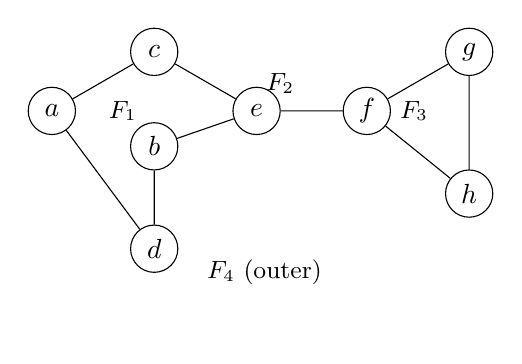
\begin{tikzpicture}[every node/.style={circle,draw,fill=white,inner sep=1.5pt,minimum size=6mm}]
\node (a) at (0,0.75) {$a$};
\node (b) at (1.3,0.3) {$b$};
\node (c) at (1.3,1.5) {$c$};
\node (d) at (1.3,-1) {$d$};
\node (e) at (2.6,0.75) {$e$};
\node (f) at (4,0.75) {$f$};
\node (g) at (5.3,1.5) {$g$};
\node (h) at (5.3,-0.3) {$h$};
\draw (a)--(c) (a)--(d) (c)--(e) (b)--(d) (b)--(e) (e)--(c) (e)--(f) (f)--(g) (f)--(h) (g)--(h);
\node[draw=none,fill=none] at (0.9,0.75) {\small $F_1$};
\node[draw=none,fill=none] at (2.9,1.1) {\small $F_2$};
\node[draw=none,fill=none] at (4.6,0.75) {\small $F_3$};
\node[draw=none,fill=none] at (2.7,-1.3) {\small $F_4$ (outer)};
\end{tikzpicture}
\end{center}
\begin{center}
\small $n=8,\ m=10,\ f=4$: check $n-m+f = 8-10+4=2$ (Euler's formula)
\end{center}

\bigskip
\begin{theorem}[Euler's formula]
For a connected plane graph with $n$ vertices, $m$ edges, $f$ faces:
\[
n-m+f = 2.
\]
\end{theorem}
\begin{proof}[Induction on $m$]
\textbf{Base case} ($m=n-1$): $G$ connected with $n-1$ edges is a tree (\S\ref{sec:12-2}), so has just one face ($f=1$):
\[
n-(n-1)+1 = 2.
\]

\medskip
\textbf{Inductive step}: let $m\ge n-1$; assume the formula for every connected plane graph with $m$ edges. Let $G$ have $n$ vertices, $m+1$ edges, $f$ faces.

Since $m+1>n-1$, $G$ is not a tree, so has a cycle $C$; let $e\in C$. The cycle $C$ separates the plane into inside/outside, so $e$'s two sides lie in \emph{different} faces. Deleting $e$ merges those two faces into one: let $H=G-e$, with $n$ vertices, $m$ edges, $f-1$ faces.

By the inductive hypothesis applied to $H$: $n-m+(f-1)=2$, i.e.\ $n-(m+1)+f=2$ -- exactly the formula for $G$.

\medskip
By induction, the formula holds for all $m\ge n-1$.
\end{proof}

\begin{corollary}[Edge bound]
For a simple, connected planar graph with $n\ge3$ vertices, $m$ edges:
\[
m \le 3n-6.
\]
\end{corollary}
\begin{proof}
Each face's boundary has $\ge3$ edges (simple graph, $n\ge3$), and each edge borders exactly $2$ face-sides, so $3f\le 2m$, i.e.\ $f\le\frac23m$. Substituting into Euler's formula: $2=n-m+f \le n-m+\frac23m = n-\frac13m$, so $m\le3n-6$.
\end{proof}

\begin{theorem}[$K_5$ is not planar]
\end{theorem}
\begin{proof}
$K_5$: $n=5$, $m=\binom52=10$. But $3n-6=9<10$ -- violates the corollary.
\end{proof}

\begin{theorem}[$K_{3,3}$ is not planar]
\end{theorem}
\begin{proof}
$K_{3,3}$: $n=6$, $m=9$, bipartite so no triangles -- every face boundary has $\ge4$ edges, giving $4f\le2m$, $f\le m/2$. Euler: $2=n-m+f\le n-m+m/2=n-m/2$, so $m\le2n-4=8<9$ -- contradiction.
\end{proof}

\bigskip
\begin{theorem}[Kuratowski's theorem, Rosen -- harder, full characterization]
$G$ is planar $\iff$ $G$ contains no subgraph that is a \emph{subdivision} of $K_5$ or $K_{3,3}$ (a copy of $K_5$/$K_{3,3}$ with edges possibly replaced by paths).
\end{theorem}
\begin{note}
The two non-planarity ``obstructions'' above ($K_5,K_{3,3}$) turn out to be the \emph{only} ones, up to subdivision -- a remarkably clean complete characterization, though the proof is well beyond this course.
\end{note}

\begin{center}
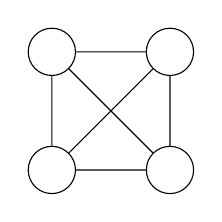
\begin{tikzpicture}[every node/.style={circle,draw,fill=white,inner sep=1.5pt,minimum size=6mm}]
\node (a) at (0,1.5) {};
\node (b) at (1.5,1.5) {};
\node (c) at (0,0) {};
\node (d) at (1.5,0) {};
\draw (a)--(b) (a)--(c) (a)--(d) (b)--(c) (b)--(d) (c)--(d);
\end{tikzpicture}
\qquad
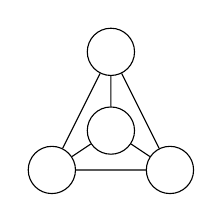
\begin{tikzpicture}[every node/.style={circle,draw,fill=white,inner sep=1.5pt,minimum size=6mm}]
\node (a) at (0.75,2) {};
\node (b) at (0,0.5) {};
\node (c) at (1.5,0.5) {};
\node (d) at (0.75,1) {};
\draw (a)--(b) (a)--(c) (a)--(d) (b)--(c) (b)--(d) (c)--(d);
\end{tikzpicture}
\end{center}
\begin{center}
\small $K_4$: a crossing drawing (left) vs.\ a planar drawing (right) -- the same graph, $K_4$ genuinely is planar
\end{center}

\begin{theorem}[Four colour theorem, Rosen -- famous, proof omitted]
Every planar graph's vertices can be $4$-coloured so that adjacent vertices differ.
\end{theorem}
\begin{note}
Conjectured 1852, proved 1976 (Appel--Haken) -- the first major theorem proved with essential computer assistance (checking $\sim1900$ unavoidable configurations), which was controversial at the time since no human could verify the proof by hand.
\end{note}

\subsection{Games on graphs (omega, advanced)}
\label{sec:12-6}
% CN 12.6 -- no direct Rosen counterpart

\subsubsection{Shannon's Switching Game}
\label{sec:12-6-1}
% CN 12.6.1

\begin{definition}[Shannon's Switching Game]
Connected graph $G$, distinguished vertices $s,t$. Players \emph{Cut}, \emph{Join} alternate turns. Cut crosses out an edge (permanently unusable); Join thickens an edge (permanently marked). Join wins as soon as thickened edges form an $s$-$t$ path; Cut wins as soon as $s,t$ are separated in the uncrossed-out graph.
\end{definition}

\begin{center}
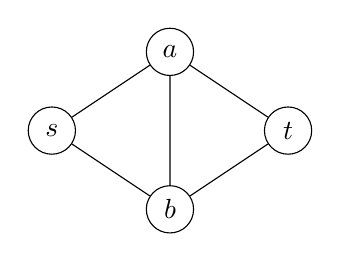
\begin{tikzpicture}[every node/.style={circle,draw,fill=white,inner sep=1.5pt,minimum size=6mm}]
\node (s) at (0,0) {$s$};
\node (a) at (1.5,1) {$a$};
\node (b) at (1.5,-1) {$b$};
\node (t) at (3,0) {$t$};
\draw (s)--(a) (s)--(b) (a)--(t) (b)--(t) (a)--(b);
\end{tikzpicture}
\end{center}
\begin{center}
\small The diamond graph used in CN's worked example of the Shannon Switching Game
\end{center}

\begin{theorem}[The game always has a winner -- no draws]
\end{theorem}
\begin{proof}
If play continues until every edge is thickened or crossed out, the thickened-edge subgraph either contains an $s$-$t$ path (Join wins) or doesn't ($s,t$ separated -- Cut wins). One of these must hold.
\end{proof}

\bigskip
\begin{theorem}[No graph favours the second player]
For every graph, either some player has a winning strategy \emph{regardless of who starts}, or the \emph{first} player (whichever role) has a winning strategy -- never the second player.
\end{theorem}
\begin{proof}[Strategy-stealing argument]
Suppose, for contradiction, the second player had a winning strategy $\sigma$ on some graph, regardless of who starts. Let the first player make \emph{any} initial move, then follow $\sigma$ as if they were "the second player" from that point on. Since making a move is never a disadvantage in this game (an extra thickened or crossed-out edge only helps, never hurts, its player -- unlike games such as Chess or Draughts), this extra first move cannot hurt them, and $\sigma$'s guarantee still applies -- so the (actual) first player wins. This contradicts $\sigma$ being a winning strategy for the second player.
\end{proof}

\begin{note}[Same strategy-stealing pattern as Chomp]
Identical in structure to the Chomp argument (\S\ref{sec:3-8}): "moving is never a disadvantage" $\Rightarrow$ the second player's supposed winning strategy could be stolen by the first player, a contradiction.
\end{note}

\begin{note}[Bridg-It]
A commercial version of this game (David Gale, 1960) played on a specific planar graph.
\end{note}

\subsubsection{Slither}
\label{sec:12-6-2}
% CN 12.6.2

\begin{definition}[Slither]
Players alternately extend a path by one edge, incident to either current endpoint, to a vertex not yet on the path. First player unable to move loses.
\end{definition}

\begin{note}
Unlike Shannon's Switching Game, Slither's outcome theory is far less settled -- CN treats it as an open exploration rather than a solved game, in contrast to the strategy-stealing argument above.
\end{note}


% ============================================================
% NOTATION SUMMARY
% ============================================================
\newpage
\section*{Notation summary}
\addcontentsline{toc}{section}{Notation summary}

\subsection*{Sets (Ch.\,1)}
\begin{longtable}{ll}
$\in,\ \notin$ & membership \\
$\emptyset,\ \{\}$ & empty set \\
$\{x : P(x)\}$ & set-builder \\
$[a,b],\ (a,b),\ [a,b),\ (a,b]$ & intervals \\
$\N,\Z,\Z^+,\Z^-,\Q,\R,\R^+,\R^-,\C$ & standard number sets \\
$|A|$ & cardinality \\
$\Sigma,\ \Sigma^n,\ \Sigma^*$ & alphabet, strings of length $n$, all strings \\
$\subseteq,\ \subsetneq,\ \supseteq$ & subset, proper subset, superset \\
$\mathcal P(A)$ & power set \\
$\binom{n}{k}$ & binomial coefficient \\
$A-B$ (or $A\setminus B$),\ $\overline{A}$ & set difference, complement \\
$\cup,\ \cap$ & union, intersection \\
$\triangle$ & symmetric difference \\
$\times,\ A^n$ & Cartesian product, $n$-fold power \\
\end{longtable}

\subsection*{Functions and relations (Ch.\,2)}
\begin{longtable}{ll}
$f:A\to B,\ f(x)$ & function declaration, value \\
$\dom(f)$ & domain \\
$i_A$ & identity function \\
$\chi_A$ & indicator/characteristic function \\
$c_a$ & constant function \\
$\lfloor x\rfloor,\ \lceil x\rceil$ & floor, ceiling \\
$f|_X$ & restriction \\
$f^{-1}$ & inverse function (or preimage, context-dependent) \\
$g\circ f$ & composition \\
$f^{(n)}$ & iterated composition \\
$e_k,\ d_k$ & encryption/decryption (cryptosystem) \\
$R \subseteq A\times B,\ xRy$ & binary relation, infix notation \\
$R(x),\ R^{-1}(y)$ & image set, inverse-image set (relation) \\
$R\circ S$ & relation composition \\
$R^{(n)},\ R^+$ & iterated relation, transitive closure \\
$[x]_R$ & equivalence class \\
$[a_{ij}]$ & matrix \\
$\wedge,\vee$ (matrices) & meet, join (zero-one matrices) \\
$\odot$ & Boolean matrix product \\
$\preceq$ & partial order \\
$\vee,\wedge$ (posets) & join (LUB), meet (GLB) \\
\end{longtable}

\subsection*{Propositional logic (Ch.\,4)}
\begin{longtable}{ll}
$T,\ F$ & truth values \\
$\neg$ & negation \\
$\wedge,\ \vee$ & conjunction, disjunction \\
$\implies,\ \iff$ & implication, biconditional \\
$\oplus$ & exclusive-or \\
$\mid$ & Sheffer stroke (NAND) \\
$\equiv$ (or $=$) & logical equivalence \\
\end{longtable}

\subsection*{Predicate logic (Ch.\,5)}
\begin{longtable}{ll}
$P(x)$ & predicate applied to a term \\
$\exists x,\ \exists x\in A$ & existential quantifier, restricted \\
$\forall x,\ \forall x\in A$ & universal quantifier, restricted \\
$\dom(f)$ & (as in Ch.\,2 -- domain of a variable/predicate argument) \\
\end{longtable}

\subsection*{Sequences and series (Ch.\,6)}
\begin{longtable}{ll}
$(a_n),\ f_n,\ (n^2:n\in\N)$ & sequence, $n$-th term, formula notation \\
$a,d$ & arithmetic sequence: first term, common difference \\
$a,r$ & geometric sequence: first term, common ratio \\
$\varphi,\psi$ & golden ratio and its conjugate (Fibonacci/Binet) \\
$O,\ \Omega,\ \Theta$ & big-O, big-Omega, big-Theta \\
$P,\ NP$ & complexity classes \\
$\sum,\ \prod$ & summation, product notation \\
$A_n$ & partial sum, Abel summation \\
$\lim_{n\to\infty}a_n,\ \varepsilon,N$ & sequence limit, $\varepsilon$-$N$ definition \\
$H_n$ & harmonic number \\
$\gamma$ & Euler's constant \\
$G(x)$ & generating function \\
\end{longtable}

\subsection*{Number theory (Ch.\,7)}
\begin{longtable}{ll}
$d\mid n,\ d\nmid n$ & $d$ divides $n$ / does not divide $n$ \\
$d\Z$ & set of multiples of $d$ \\
$n\bmod d$ & remainder of $n$ on division by $d$ \\
$\lfloor n/d\rfloor$ & quotient of $n$ on division by $d$ \\
$\gcd(a,b),\ \lcmop(a,b)$ & greatest common divisor, least common multiple \\
$\mathrm{CD}(x,y)$ & set of common divisors of $x,y$ \\
$m\Z+n\Z$ & integer linear combinations $\{xm+yn : x,y\in\Z\}$ \\
$(a,x,y),\ (b,z,w)$ & EEA triples, $a=xm+yn,\ b=zm+wn$ \\
$a\equiv b\pmod n$ & congruence mod $n$: $n\mid(a-b)$ \\
$[a],\ a+n\Z$ & residue class of $a$ mod $n$ \\
$\Z_n$ & $\{0,\dots,n-1\}$ with arithmetic mod $n$ \\
$\Z_n^*$ & elements of $\Z_n$ with a multiplicative inverse \\
$x^{-1}$ (mod $n$) & multiplicative inverse of $x$ in $\Z_n$ \\
$\varphi(n)$ & Euler totient function, $|\Z_n^*|$ \\
$\mathrm{ds}(n),\ \mathrm{ads}(n)$ & digital sum, alternating digital sum \\
$\log_a y$ (mod $n$) & discrete logarithm: $x$ with $a^x\equiv y\pmod n$ \\
$p,q$ & primes (generic; RSA's two secret primes in examples) \\
$e,d$ & RSA public/private exponents \\
$x_A,x_B,y_A,y_B$ & Diffie--Hellman private/public numbers \\
$k_{AB},\ k_{BA}$ & Diffie--Hellman shared key \\
\end{longtable}

\subsection*{Counting \& combinatorics (Ch.\,8)}
\begin{longtable}{ll}
$\lceil x\rceil,\ \lfloor x\rfloor$ & ceiling, floor (pigeonhole bounds) \\
$R(3,3)$ & Ramsey number \\
$\bigcup,\bigcap$ (inclusion-exclusion) & union/intersection over index sets, \S\ref{sec:8-3} \\
$D_n$ & derangement count \\
$(n)_r,\ {}_nP_r,\ P(n,r)$ & falling factorial, permutations \\
$\binom{n}{r},\ {}_nC_r$ & binomial coefficient, combinations \\
$\binom{r+n-1}{r}$ & unordered selection with replacement (stars and bars) \\
$S(n,k)$ & Stirling number of the second kind \\
\end{longtable}

\subsection*{Proof and general notation (Ch.\,3, throughout)}
\begin{longtable}{ll}
$\blacksquare$ & end of proof \\
$\mid$ (number theory) & divides ($a\mid b$) \\
$\Rightarrow$ (proof steps) & logical consequence within a proof \\
\end{longtable}

\end{document}